% Options for packages loaded elsewhere
\PassOptionsToPackage{unicode}{hyperref}
\PassOptionsToPackage{hyphens}{url}
\PassOptionsToPackage{dvipsnames,svgnames,x11names}{xcolor}
%
\documentclass[
  letterpaper,
]{book}

\usepackage{amsmath,amssymb}
\usepackage{iftex}
\ifPDFTeX
  \usepackage[T1]{fontenc}
  \usepackage[utf8]{inputenc}
  \usepackage{textcomp} % provide euro and other symbols
\else % if luatex or xetex
  \usepackage{unicode-math}
  \defaultfontfeatures{Scale=MatchLowercase}
  \defaultfontfeatures[\rmfamily]{Ligatures=TeX,Scale=1}
\fi
\usepackage{lmodern}
\ifPDFTeX\else  
    % xetex/luatex font selection
\fi
% Use upquote if available, for straight quotes in verbatim environments
\IfFileExists{upquote.sty}{\usepackage{upquote}}{}
\IfFileExists{microtype.sty}{% use microtype if available
  \usepackage[]{microtype}
  \UseMicrotypeSet[protrusion]{basicmath} % disable protrusion for tt fonts
}{}
\makeatletter
\@ifundefined{KOMAClassName}{% if non-KOMA class
  \IfFileExists{parskip.sty}{%
    \usepackage{parskip}
  }{% else
    \setlength{\parindent}{0pt}
    \setlength{\parskip}{6pt plus 2pt minus 1pt}}
}{% if KOMA class
  \KOMAoptions{parskip=half}}
\makeatother
\usepackage{xcolor}
\setlength{\emergencystretch}{3em} % prevent overfull lines
\setcounter{secnumdepth}{5}
% Make \paragraph and \subparagraph free-standing
\ifx\paragraph\undefined\else
  \let\oldparagraph\paragraph
  \renewcommand{\paragraph}[1]{\oldparagraph{#1}\mbox{}}
\fi
\ifx\subparagraph\undefined\else
  \let\oldsubparagraph\subparagraph
  \renewcommand{\subparagraph}[1]{\oldsubparagraph{#1}\mbox{}}
\fi

\providecommand{\tightlist}{%
  \setlength{\itemsep}{0pt}\setlength{\parskip}{0pt}}\usepackage{longtable,booktabs,array}
\usepackage{calc} % for calculating minipage widths
% Correct order of tables after \paragraph or \subparagraph
\usepackage{etoolbox}
\makeatletter
\patchcmd\longtable{\par}{\if@noskipsec\mbox{}\fi\par}{}{}
\makeatother
% Allow footnotes in longtable head/foot
\IfFileExists{footnotehyper.sty}{\usepackage{footnotehyper}}{\usepackage{footnote}}
\makesavenoteenv{longtable}
\usepackage{graphicx}
\makeatletter
\def\maxwidth{\ifdim\Gin@nat@width>\linewidth\linewidth\else\Gin@nat@width\fi}
\def\maxheight{\ifdim\Gin@nat@height>\textheight\textheight\else\Gin@nat@height\fi}
\makeatother
% Scale images if necessary, so that they will not overflow the page
% margins by default, and it is still possible to overwrite the defaults
% using explicit options in \includegraphics[width, height, ...]{}
\setkeys{Gin}{width=\maxwidth,height=\maxheight,keepaspectratio}
% Set default figure placement to htbp
\makeatletter
\def\fps@figure{htbp}
\makeatother
% definitions for citeproc citations
\NewDocumentCommand\citeproctext{}{}
\NewDocumentCommand\citeproc{mm}{%
  \begingroup\def\citeproctext{#2}\cite{#1}\endgroup}
\makeatletter
 % allow citations to break across lines
 \let\@cite@ofmt\@firstofone
 % avoid brackets around text for \cite:
 \def\@biblabel#1{}
 \def\@cite#1#2{{#1\if@tempswa , #2\fi}}
\makeatother
\newlength{\cslhangindent}
\setlength{\cslhangindent}{1.5em}
\newlength{\csllabelwidth}
\setlength{\csllabelwidth}{3em}
\newenvironment{CSLReferences}[2] % #1 hanging-indent, #2 entry-spacing
 {\begin{list}{}{%
  \setlength{\itemindent}{0pt}
  \setlength{\leftmargin}{0pt}
  \setlength{\parsep}{0pt}
  % turn on hanging indent if param 1 is 1
  \ifodd #1
   \setlength{\leftmargin}{\cslhangindent}
   \setlength{\itemindent}{-1\cslhangindent}
  \fi
  % set entry spacing
  \setlength{\itemsep}{#2\baselineskip}}}
 {\end{list}}
\usepackage{calc}
\newcommand{\CSLBlock}[1]{\hfill\break\parbox[t]{\linewidth}{\strut\ignorespaces#1\strut}}
\newcommand{\CSLLeftMargin}[1]{\parbox[t]{\csllabelwidth}{\strut#1\strut}}
\newcommand{\CSLRightInline}[1]{\parbox[t]{\linewidth - \csllabelwidth}{\strut#1\strut}}
\newcommand{\CSLIndent}[1]{\hspace{\cslhangindent}#1}

\widowpenalty=10000         % avoid widows
\clubpenalty=10000          % avoid orphans
\interfootnotelinepenalty=10000 % avoid footnote splitting across pages
\usepackage[scale=3.5]{ccicons}
\makeatletter
\@ifpackageloaded{bookmark}{}{\usepackage{bookmark}}
\makeatother
\makeatletter
\@ifpackageloaded{caption}{}{\usepackage{caption}}
\AtBeginDocument{%
\ifdefined\contentsname
  \renewcommand*\contentsname{Table of contents}
\else
  \newcommand\contentsname{Table of contents}
\fi
\ifdefined\listfigurename
  \renewcommand*\listfigurename{List of Figures}
\else
  \newcommand\listfigurename{List of Figures}
\fi
\ifdefined\listtablename
  \renewcommand*\listtablename{List of Tables}
\else
  \newcommand\listtablename{List of Tables}
\fi
\ifdefined\figurename
  \renewcommand*\figurename{Figure}
\else
  \newcommand\figurename{Figure}
\fi
\ifdefined\tablename
  \renewcommand*\tablename{Table}
\else
  \newcommand\tablename{Table}
\fi
}
\@ifpackageloaded{float}{}{\usepackage{float}}
\floatstyle{ruled}
\@ifundefined{c@chapter}{\newfloat{codelisting}{h}{lop}}{\newfloat{codelisting}{h}{lop}[chapter]}
\floatname{codelisting}{Listing}
\newcommand*\listoflistings{\listof{codelisting}{List of Listings}}
\makeatother
\makeatletter
\makeatother
\makeatletter
\@ifpackageloaded{caption}{}{\usepackage{caption}}
\@ifpackageloaded{subcaption}{}{\usepackage{subcaption}}
\makeatother

\usepackage{hyphenat}
\usepackage{ifthen}
\usepackage{calc}
\usepackage{calculator}


\usepackage{geometry}

\usepackage{graphicx}
\usepackage{geometry}
\usepackage{afterpage}
\usepackage{tikz}
\usetikzlibrary{calc}
\usetikzlibrary{fadings}
\usepackage[pagecolor=none]{pagecolor}


% Set the titlepage font families




\usepackage{fontspec}
\newfontfamily{\titlepagefooterfont}{QTHelvetCnd.otf}



% Set the coverpage font families

\ifLuaTeX
\usepackage[bidi=basic]{babel}
\else
\usepackage[bidi=default]{babel}
\fi
\babelprovide[main,import]{english}
% get rid of language-specific shorthands (see #6817):
\let\LanguageShortHands\languageshorthands
\def\languageshorthands#1{}
\ifLuaTeX
  \usepackage{selnolig}  % disable illegal ligatures
\fi
\usepackage{bookmark}

\IfFileExists{xurl.sty}{\usepackage{xurl}}{} % add URL line breaks if available
\urlstyle{same} % disable monospaced font for URLs
\hypersetup{
  pdftitle={Through the Looking Glass: I. Why Cross-Fertilize?},
  pdfauthor={Curtis M. Lively},
  pdflang={en},
  pdfsubject={evolutionary biology},
  pdfkeywords={biology, evolution, sexual reproduction, evolutionary
biology},
  colorlinks=true,
  linkcolor={blue},
  filecolor={Maroon},
  citecolor={Blue},
  urlcolor={Blue},
  pdfcreator={LaTeX via pandoc}}

\title{Through the Looking Glass: I. Why Cross-Fertilize?}
\author{Curtis M. Lively}
\date{2024}

\begin{document}
%%%%% begin titlepage extension code

  \begin{frontmatter}

\begin{titlepage}
% This is a combination of Pandoc templating and LaTeX
% Pandoc templating https://pandoc.org/MANUAL.html#templates
% See the README for help

\thispagestyle{empty}

\newgeometry{top=-100in}

% Page color

\newcommand{\coverauthorstyle}[1]{{#1}}

\begin{tikzpicture}[remember picture, overlay, inner sep=0pt, outer sep=0pt]

\tikzfading[name=fadeout, inner color=transparent!0,outer color=transparent!100]
\tikzfading[name=fadein, inner color=transparent!100,outer color=transparent!0]
\node[anchor=south west, rotate=0.0, opacity=1.0] at ($(current page.south west)+(0.0, 0.0)$) {
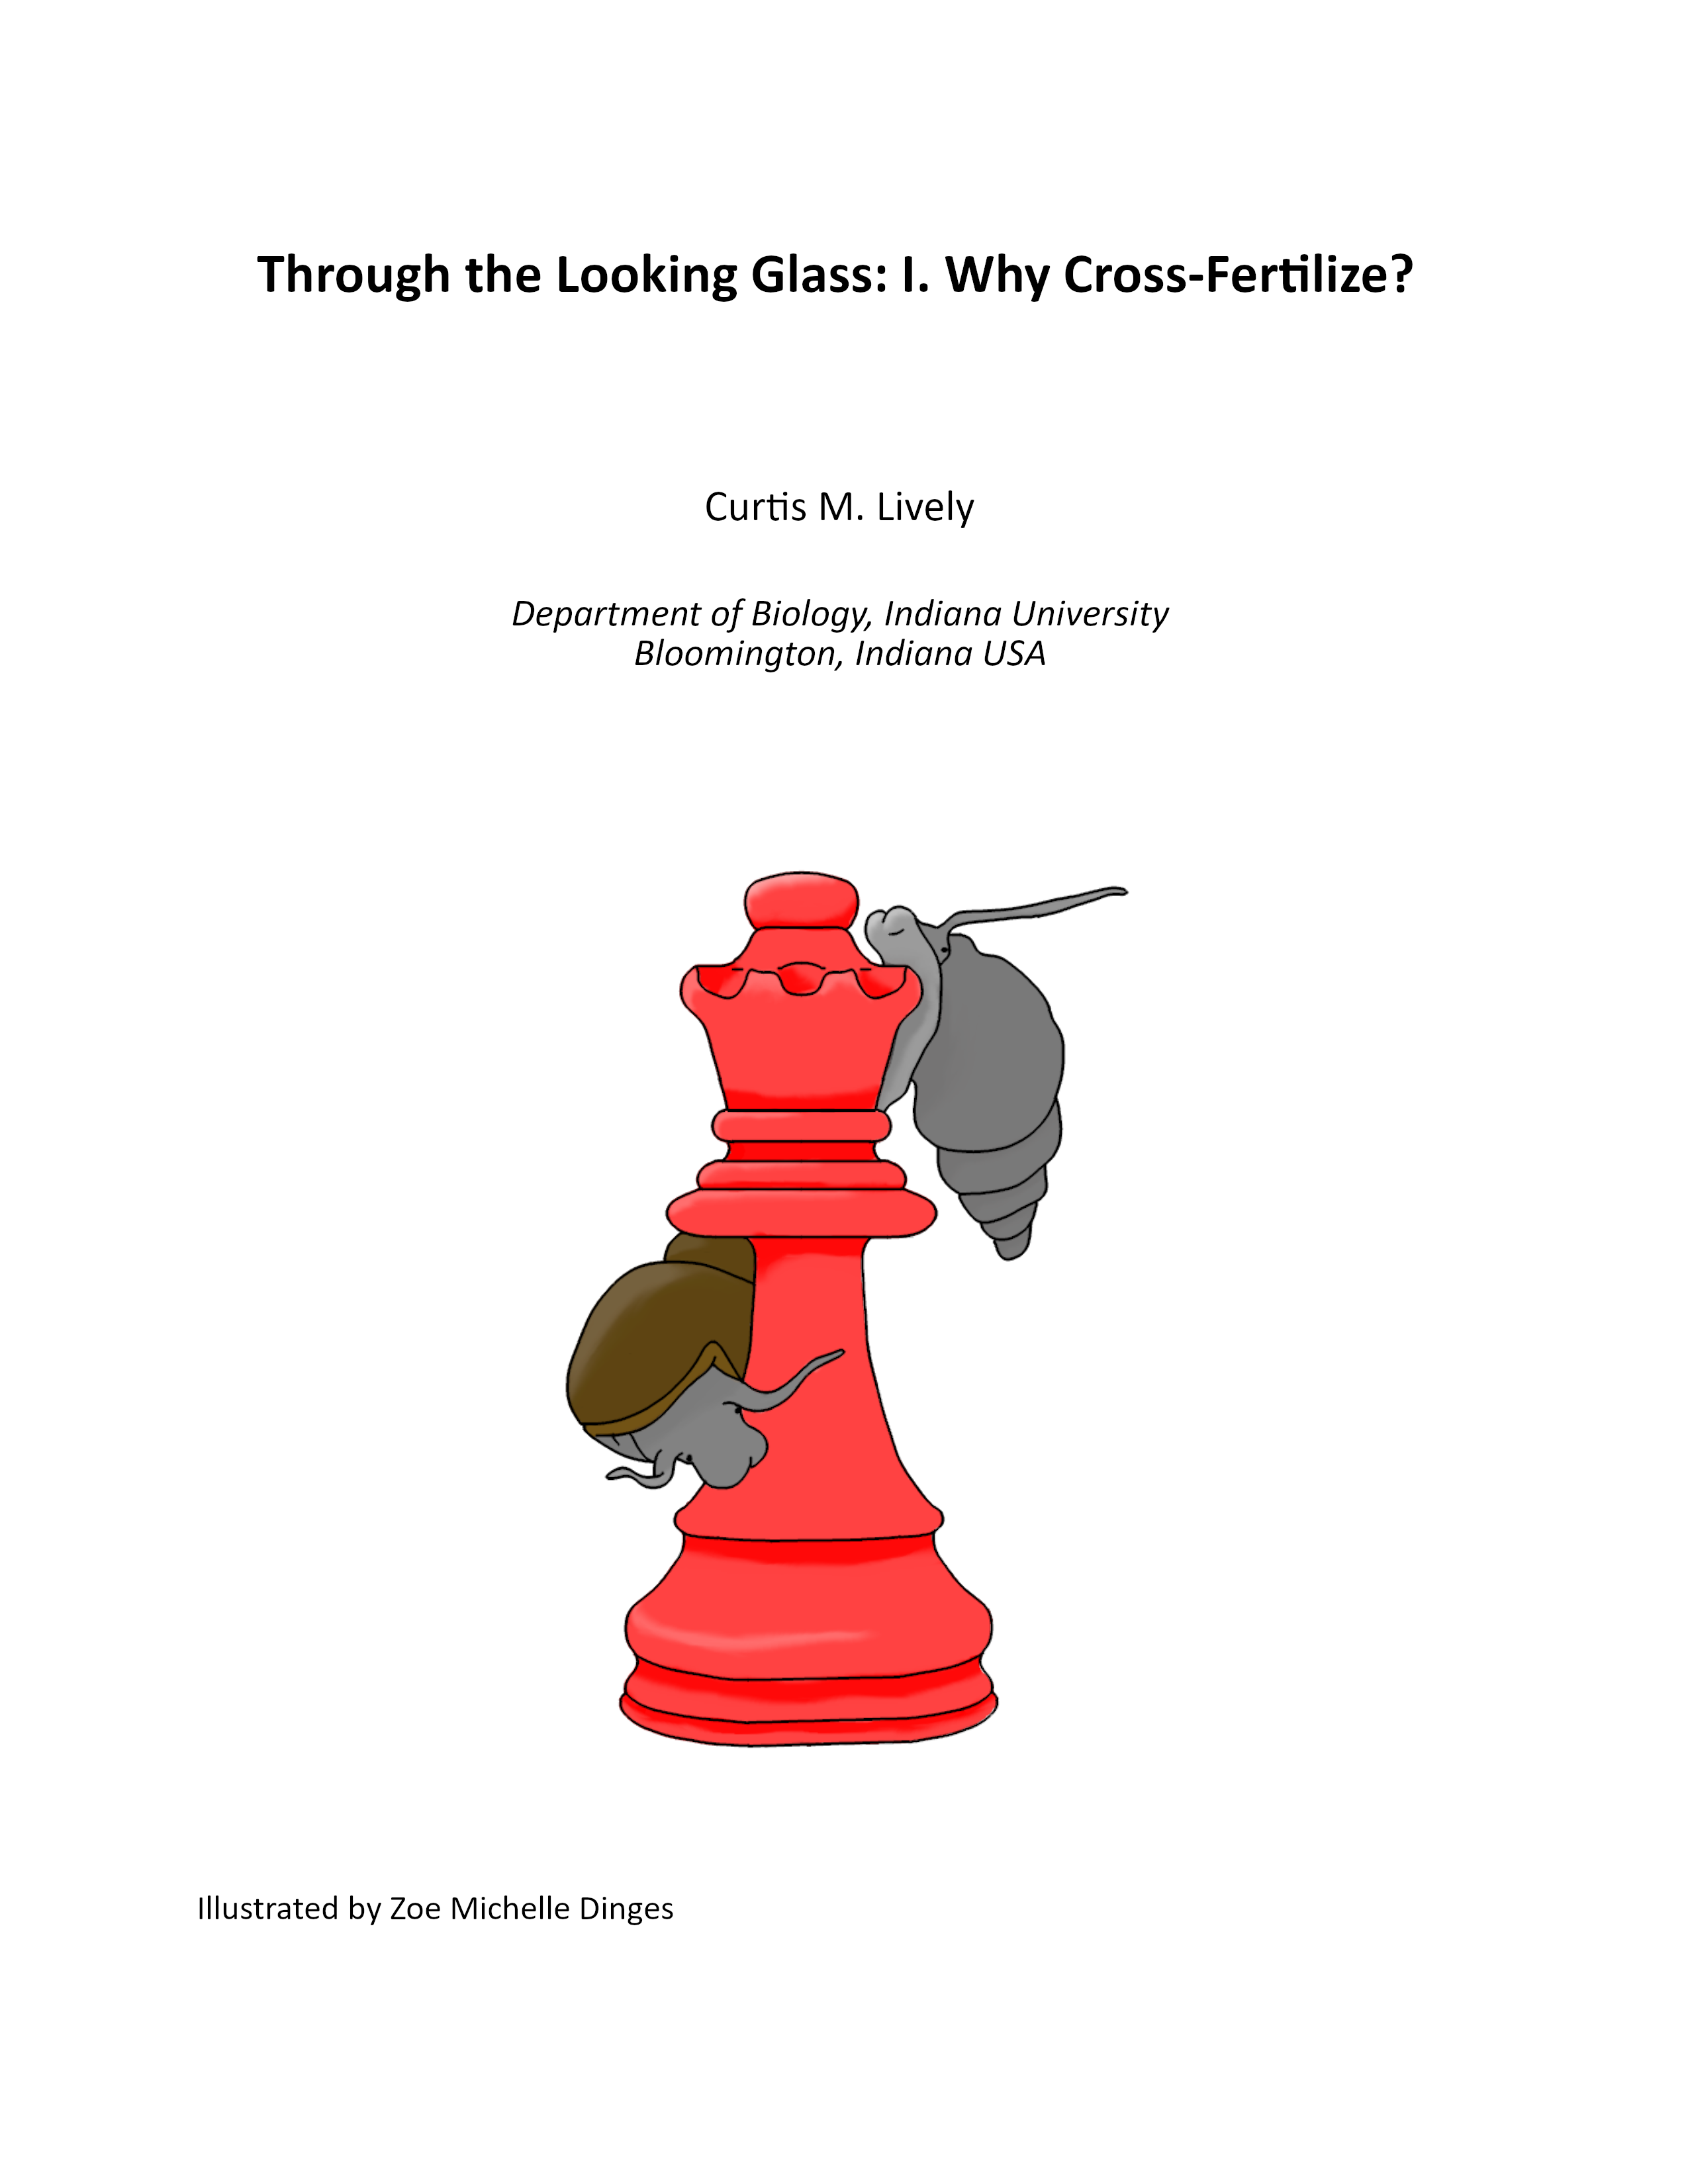
\includegraphics[width=\paperwidth, keepaspectratio]{images/cover.png}};


\end{tikzpicture}
\clearpage
\restoregeometry
%%% TITLE PAGE START

% Set up alignment commands
%Page
\newcommand{\titlepagepagealign}{
\ifthenelse{\equal{left}{right}}{\raggedleft}{}
\ifthenelse{\equal{left}{center}}{\centering}{}
\ifthenelse{\equal{left}{left}}{\raggedright}{}
}


\newcommand{\titleandsubtitle}{
% Title and subtitle
{{\Huge{\textbf{\nohyphens{Through the Looking Glass: I. Why
Cross-Fertilize?}}}}\par
}%
}
\newcommand{\titlepagetitleblock}{
\titleandsubtitle
}

\newcommand{\authorstyle}[1]{{\fontsize{20}{24.0}\selectfont
#1}}

\newcommand{\affiliationstyle}[1]{{#1}}

\newcommand{\titlepageauthorblock}{
{\authorstyle{\nohyphens{Curtis M. Lively}\\}}
}

\newcommand{\titlepageaffiliationblock}{}
\newcommand{\headerstyled}{%
{}
}
\newcommand{\footerstyled}{%
{\fontsize{15}{18.0}\selectfont
Indiana University Bloomington Libraries Publishing\\
Bloomington, Indiana}
}
\newcommand{\datestyled}{%
{2024}
}


\newcommand{\titlepageheaderblock}{\headerstyled}

\newcommand{\titlepagefooterblock}{
\footerstyled
}

\newcommand{\titlepagedateblock}{
\datestyled
}

%set up blocks so user can specify order
\newcommand{\titleblock}{{

{\titlepagetitleblock}
}

\vspace{1.5cm}
}

\newcommand{\authorblock}{{\titlepageauthorblock}

\vspace{2\baselineskip}
}

\newcommand{\affiliationblock}{{\titlepageaffiliationblock}

\vspace{2\baselineskip}
}

\newcommand{\logoblock}{{\includegraphics[width=0.5\paperwidth]{images/iublpub\_logo.png}}

\vspace{1\baselineskip}
}

\newcommand{\footerblock}{{\titlepagefooterfont
\titlepagefooterblock}

\vspace{1pt}
}

\newcommand{\dateblock}{{\titlepagedateblock}

\vspace{0pt}
}

\newcommand{\headerblock}{}
\newgeometry{top=3in,bottom=1.5in,right=1in,left=1in}

\thispagestyle{empty} % no page numbers on titlepages


\newlength{\minipagewidth}
\setlength{\minipagewidth}{\textwidth}
\raggedright % single minipage
% [position of box][box height][inner position]{width}
% [s] means stretch out vertically; assuming there is a vfill
\begin{minipage}[b][\textheight][s]{\minipagewidth}
\titlepagepagealign
\titleblock

\authorblock

\Large Illustrated by Zoe Michelle Dinges

\vfill

\logoblock

\footerblock
\par

\end{minipage}\ifthenelse{\equal{}{right} \OR \equal{}{leftright} }{
\hspace{\B}
\vrulecode}{}
\clearpage
\restoregeometry
%%% TITLE PAGE END

\null\vfill
\begin{flushleft}
\thispagestyle{empty}
Indiana University Bloomington Libraries Publishing\\
1320 E. Tenth Street\\
Bloomington, IN 47405
\vspace{5mm}

© 2024 Curtis M. Lively\\
Illustrations © 2024 Zoe Michelle Dinges

\vspace{3mm}
\ccby

\textit{Through the Looking Glass: I. Why Cross-Fertilize?} © 2024 by Curtis M. Lively and Zoe Michelle Dinges is licensed under Attribution 4.0 International. To view a copy of this license, visit \url{http://creativecommons.org/licenses/by/4.0/}

\textbf{You are free to:}
\begin{itemize}
\tightlist
\item
  \textbf{Share---}copy and redistribute the material in any medium or format for any purpose, even commercially.\\
\item
  \textbf{Adapt---}remix, transform, and build upon the material for any purpose, even commercially.
\end{itemize}

The licensor cannot revoke these freedoms as long as you follow the license terms.

\textbf{Under the following terms:}
\begin{itemize}
\tightlist
\item
  \textbf{Attribution---}You must give
  \href{https://creativecommons.org/licenses/by/4.0/\#ref-appropriate-credit}{appropriate credit}, provide a link to the license, and
  \href{https://creativecommons.org/licenses/by/4.0/\#ref-indicate-changes}{indicate if changes were made}. You may do so in any reasonable manner, but not in any way that suggests the licensor endorses you or your use.\\
\item
  \textbf{No additional restrictions---}You may not apply legal terms or
  \href{https://creativecommons.org/licenses/by/4.0/\#ref-technological-measures}{technological measures} that legally restrict others from doing anything the license permits.
\end{itemize}

\textbf{Notices:}

\begin{itemize}
\tightlist
\item
  You do not have to comply with the license for elements of the material in the public domain or where your use is permitted by an applicable
  \href{https://creativecommons.org/licenses/by/4.0/\#ref-exception-or-limitation}{exception or limitation}.\\
\item
  No warranties are given. The license may not give you all of the permissions necessary for your intended use. For example, other rights such as
  \href{https://creativecommons.org/licenses/by/4.0/\#ref-publicity-privacy-or-moral-rights}{publicity, privacy, or moral rights} may limit how you use the material.
\end{itemize}

\vspace{5mm}
DOI: \href{https://doi.org/10.5967/gbd3-ka07}{10.5967/gbd3-ka07}
\end{flushleft}

\clearpage
\end{titlepage}
\setcounter{page}{1}
\end{frontmatter}

%%%%% end titlepage extension code

\renewcommand*\contentsname{Contents}
{
\hypersetup{linkcolor=}
\setcounter{tocdepth}{2}
\tableofcontents
}
\listoffigures
\listoftables
\mainmatter
\bookmarksetup{startatroot}

\chapter*{Front Matter}\label{front-matter}
\addcontentsline{toc}{chapter}{Front Matter}

\markboth{Front Matter}{Front Matter}

\section*{Abstract}\label{abstract}
\addcontentsline{toc}{section}{Abstract}

\markright{Abstract}

The following pages represent the first volume of a book. The main goal
is to introduce the evolutionary problem of sexual reproduction with a
focus on competition between sexual and asexual females. But I also
incorporate some ideas on genetic polymorphism and phenotypic plasticity
with the goal of exploring ``variation strategies'' more generally.
Finally, I try to weave in some history of the field along with some
philosophy of science.

\section*{Acknowledgements}\label{acknowledgements}
\addcontentsline{toc}{section}{Acknowledgements}

\markright{Acknowledgements}

I gratefully acknowledge helpful comments from Amrita Bhattacharya, Zoe
Dinges, Kara Million, Deanna Soper, Mike Wade, Jukka Jokela, Dorota
Paczesniak, Steve Howard, Lynda Delph, Clark Craddock, Robert
Vrijenhoek, Jan McKenzie, Mike Winterbourn, Stuart West, Bob Holt, Oren
Harman, and especially Maurine Neiman and her lab group at the
University of Iowa. Additional comments are welcome by
\href{mailto:clively@indiana.edu}{email}.

Special thanks to Zoe Michelle Dinges (ZMD). Zoe redrew the figures, and
she created the beautiful illustrations.

Special thanks also to Adam Mazel of Indiana University Libraries for
preparing the document for online publication. I am also grateful to
Bart Zijlstra and Gabe Harp for permission to use their original
photographs.

This project was supported by the NSF OPUS program for the synthesis of
biological research (DEB-1906465). I am also grateful to the Institute
for Advanced Study in Berlin (Wissenschaftskolleg zu Berlin) for my stay
as a ``partner'' during 2022-2023.

\section*{How to Use}\label{how-to-use}
\addcontentsline{toc}{section}{How to Use}

\markright{How to Use}

\begin{itemize}
\tightlist
\item
  \textbf{How to Access this Book in Other Formats}

  \begin{itemize}
  \tightlist
  \item
    \textbf{DOCX:} click in the lefthand sidebar of the
    \href{https://iulibscholcomm.github.io/through-the-looking-glass/}{HTML
    version} or click
    \href{https://iulibscholcomm.github.io/through-the-looking-glass/Through-the-Looking-Glass--I.-Why-Cross-Fertilize-.docx}{here}.

    \begin{itemize}
    \tightlist
    \item
      DOCX's benefits include reusability (revising, remixing, etc.) for
      those with Microsoft Word
    \end{itemize}
  \item
    \textbf{EPUB:} click in the lefthand sidebar of the
    \href{https://iulibscholcomm.github.io/through-the-looking-glass/}{HTML
    version} or click
    \href{https://iulibscholcomm.github.io/through-the-looking-glass/Through-the-Looking-Glass--I.-Why-Cross-Fertilize-.epub}{here}.

    \begin{itemize}
    \tightlist
    \item
      EPUB's benefits include universal accessibility, manipulability
      (via eReader options), dynamic media, interactivity, reflowable
      text, and offline reading
    \end{itemize}
  \item
    \textbf{HTML:} click
    \href{https://iulibscholcomm.github.io/through-the-looking-glass/}{here}.

    \begin{itemize}
    \tightlist
    \item
      HTML's benefits include machine readability, dynamic media,
      interactivity,
      \href{https://en.wikipedia.org/wiki/Reflowable_document}{reflowable
      text}, online reading, and small file size
    \end{itemize}
  \item
    \textbf{TeX:} click `` View source'' in the righthand sidebar of the
    \href{https://iulibscholcomm.github.io/through-the-looking-glass/}{HTML
    version}; then from ``Files'' in the lefthand sidebar, select
    ``Through-the-Looking-Glass--I.-Why-Cross-Fertilize-.tex.''

    \begin{itemize}
    \tightlist
    \item
      (La)TeX's benefits include advanced document formatting and
      typesetting
    \end{itemize}
  \item
    \textbf{PDF:} click in the lefthand sidebar of the
    \href{https://iulibscholcomm.github.io/through-the-looking-glass/}{HTML
    version} or click
    \href{https://iulibscholcomm.github.io/through-the-looking-glass/Through-the-Looking-Glass--I.-Why-Cross-Fertilize-.pdf}{here}.

    \begin{itemize}
    \tightlist
    \item
      PDF's benefits include printability of physical copies
    \end{itemize}
  \item
    \textbf{Quarto Markdown (QMD):} click `` View source'' in the
    righthand sidebar of the
    \href{https://iulibscholcomm.github.io/through-the-looking-glass/}{HTML
    version}.

    \begin{itemize}
    \tightlist
    \item
      QMD's benefits include reusability (revising, remixing,
      reformatting, repurposing, etc.) via a universal format
    \end{itemize}
  \end{itemize}
\item
  \textbf{How to Use Social Media to Share or Draw Attention to this
  Book}

  \begin{itemize}
  \tightlist
  \item
    Click in the lefthand sidebar of the
    \href{https://iulibscholcomm.github.io/through-the-looking-glass/}{HTML
    version} and select Twitter (now X), Facebook, or LinkedIn.
  \end{itemize}
\item
  \textbf{How to Report a Problem (Technological, Accessibility, or
  Textual) with this Book}

  \begin{itemize}
  \tightlist
  \item
    Click ``Report an Issue'' in the righthand sidebar of the
    \href{https://iulibscholcomm.github.io/through-the-looking-glass/}{HTML
    version}; then complete and submit the bug report.
  \end{itemize}
\end{itemize}

To learn more about how to use this book, see
\href{https://quarto.org/docs/guide/}{Quarto's Guide}, or simply try its
features!

\section*{How to Cite}\label{how-to-cite}
\addcontentsline{toc}{section}{How to Cite}

\markright{How to Cite}

Lively, C.M. (2024).
\href{https://doi.org/10.5967/GBD3-KA07}{\emph{Through the Looking
Glass: I. Why Cross-Fertilize?}} Indiana University Bloomington
Libraries Publishing.

\bookmarksetup{startatroot}

\chapter{Why Sex?}\label{sec-why-sex}

\begin{center}
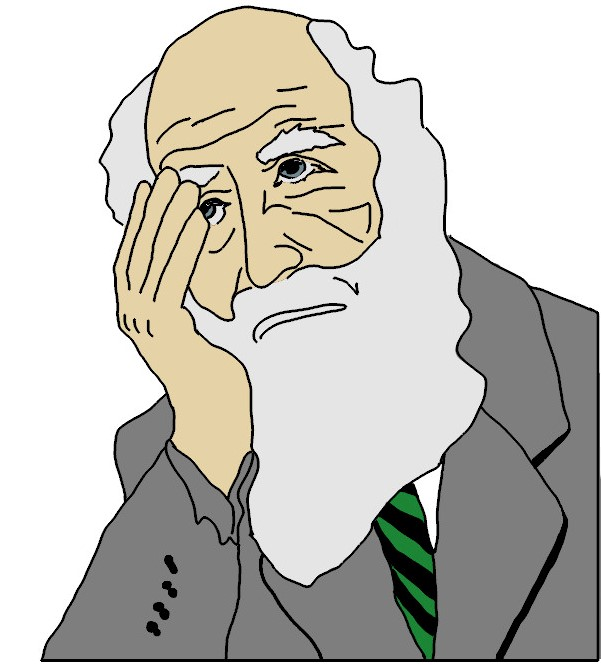
\includegraphics[width=0.4\textwidth,height=\textheight]{images/fig1-1.jpeg}
\end{center}

\section{The Question}\label{the-question}

Most PhD programs require that students pass a preliminary examination.
This was certainly true in my case. I was a PhD student at the
University of Arizona studying rocky intertidal communities in the
Northern Gulf of California. But the exams were not focused on our
research. They were ``depth-of-knowledge'' exams. My question from
Professor Astrid Kodric-Brown instructed me to read the preface of G.C.
Williams' (\citeproc{ref-williams1975a}{1975}) book, \emph{Sex and
Evolution}, which contains the following text: ``This book is written
from a conviction that the prevalence of sexual reproduction in higher
plants and animals is inconsistent with current evolutionary
theory.\ldots{} Many well-informed readers may disagree with much of my
reasoning, but I hope to at least convince them that here is a crisis at
hand in evolutionary biology.''

The question was something like this: ``Why does Williams think that
sexual reproduction poses a crisis for evolutionary biology, and what is
the solution?'' A crisis? That was news to me. How could there be a
crisis in evolutionary biology 40+ years after the modern synthesis? My
graduate course in theoretical population genetics did not mention any
crises. I was not convinced. And a little freaked out.

The structure of our exams was very loose. I don't remember having a
deadline to produce a written answer, but I do remember that I spent
several months on just this one question. During much of this time, I
was doing field work in Sonora, Mexico, sometimes under very harsh
conditions. But the more I studied the question, the more fascinated I
became. I came to think that there was, indeed, a very real anomaly
presented by sexual reproduction. Williams was right. Perhaps I was
especially interested in this anomaly because I had read Thomas Kuhn's
book, \emph{The Structure of Scientific Revolutions}, as an
undergraduate at Glendale Community College. Kuhn
(\citeproc{ref-kuhn1970a}{1970}) made the case that dissecting anomalies
can lead to interesting advances and that made sense to me. While I
eventually produced an essay to address the question, the answer felt
incomplete. I wanted to know more. There were many hypotheses, but there
was no clear general explanation. Many years later, I am still working
on my prelim question. This book is my revised answer.

\section{The Problem}\label{the-problem}

There are many problems associated with sexual reproduction, including
the time spent finding mates and the risk of contracting sexually
transmitted disease (review in \citeproc{ref-lehtonen2012a}{Lehtonen
\emph{et al.} 2012}). However, while important, these costs do not form
the core of the paradox. Historically, the paradox of sex stems from two
things: (1) the cost of meiosis, and (2) the cost of producing males.

\subsection{The cost of meiosis: reduced
relatedness}\label{the-cost-of-meiosis-reduced-relatedness}

The ``cost of meiosis'' was proposed by George Williams
(\citeproc{ref-williams1975a}{1975}). His idea was simply that females
are only half as related to their outcrossed offspring as they are to
their self-fertilized or parthenogenetic offspring.\footnote{It is not
  meiosis \emph{per se} that is costly. As Williams realized, the cost
  stems from the reduction in relatedness between parent and outcrossed
  offspring. Indeed, in a later paper, Williams
  (\citeproc{ref-williams1975a}{1975}) refers to the cost of meiosis as
  the ``paradox of kin selection.'' Why should organisms invest
  resources in kin with a relatively low level of relatedness, \(r\)
  (outcrossed progeny: \(r = 0.5\)), rather than in self-fertilized kin
  with a high level of relatedness (\(r = 1\))? (See
  \citeproc{ref-dagg2016a}{Dagg 2016}.)} (See
\hyperref[sec-glossary]{Glossary} for condensed definitions.) Williams'
idea also had theoretical support, as R.A. Fisher
(\citeproc{ref-fisher1941a}{1941}) had already shown that an allele
causing self-fertilization would rapidly spread to fixation, barring
severe inbreeding depression. So, why cross-fertilize? The persistence
of cross-fertilization despite the cost of meiosis formed a paradox.
This paradox created the crisis that Williams saw in evolutionary
biology.

\subsection{The cost of males}\label{the-cost-of-males}

The other way to look at the problem was proposed by John Maynard Smith
(\citeproc{ref-maynard1971a}{1971}, \citeproc{ref-maynard1978a}{1978}).
Here the issue is not relatedness. The problem stems rather from the
difference between sexuals and asexuals in their per-capita birth rates
(Figure~\ref{fig-1.1}). Imagine a population of sexual individuals at
carrying capacity (\(K_{sex}\)). At \(K_{sex}\) the sexual females are,
by definition, simply replacing themselves. This means that each sexual
female is, on average, producing one son and one daughter. Both sons and
daughters contribute genetically to the next generation, but only
females give birth. Now, consider a mutation in a single female that
causes her to reproduce asexually. She gives birth to two daughters
instead of one daughter and one son. These two asexually produced
daughters both give birth to two more daughters. Hence, after just two
generations, the asexual female has four granddaughters, while the
average sexual female has just one granddaughter (Figure~\ref{fig-1.1}).
This asymmetry should lead to the rapid replacement of sexual females by
asexual females (Figure~\ref{fig-1.2}). And by ``rapid,'' I mean within
tens of generations, even for very large populations
(\citeproc{ref-lively1996a}{Lively 1996}). We thus seek a selective
force that can give an advantage to sexual reproduction on a very short
time scale.

\begin{figure}

\centering{

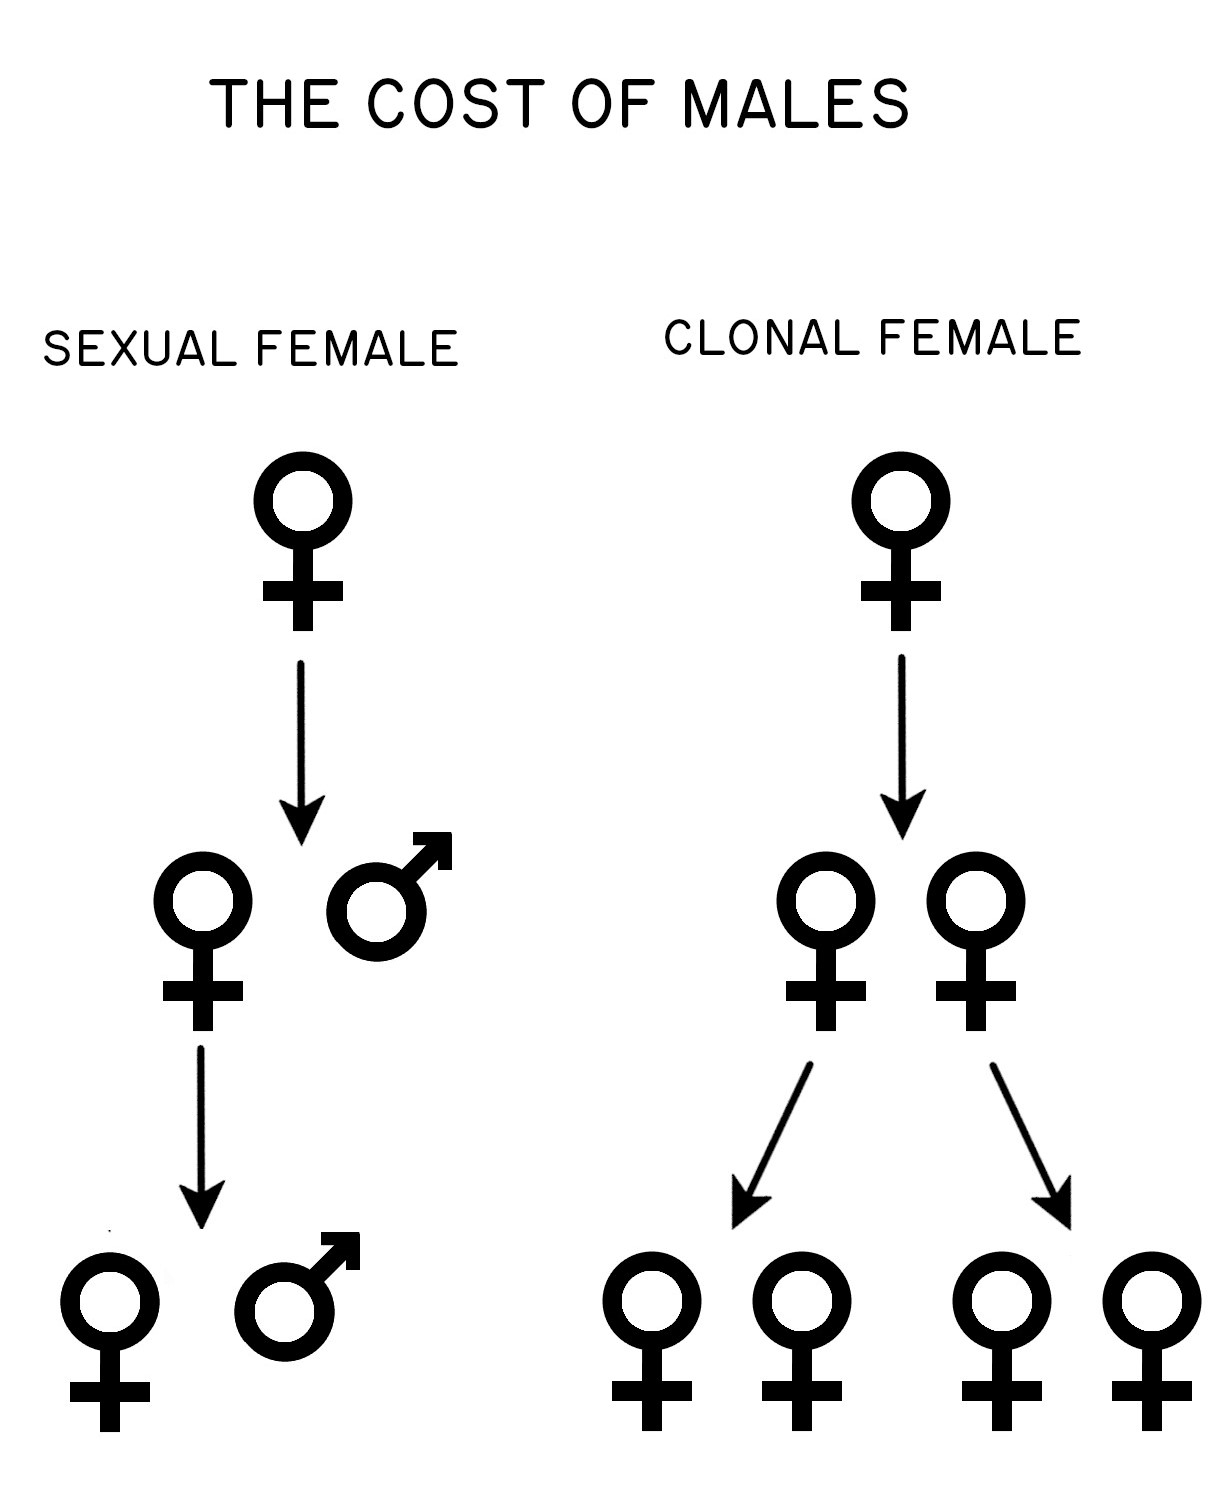
\includegraphics[width=0.5\textwidth,height=\textheight]{images/fig1-2.jpg}

}

\caption[The cost of males]{\label{fig-1.1}The cost of males. Imagine a
single clonal female in a sexual population at carrying capacity,
\(K_{sex}\). At \(K_{sex}\), the sexual females are, on average,
producing one daughter and one son. In contrast, the clonal female
produces two daughters and four granddaughters. Hence, the clonal
lineage should rapidly eliminate the sexual population
(Figure~\ref{fig-1.2}). However, in nature, asexual reproduction is very
rare in both plants (\citeproc{ref-whitton2008a}{Whitton \emph{et al.}
2008}) and animals (\citeproc{ref-vrijenhoek1998a}{Vrijenhoek 1998}).
Hence the paradox. Why is sexual reproduction so costly and yet so
common?}

\end{figure}%

Several assumptions went into Maynard Smith's model for the cost of
males. In particular, he assumed that sexual females and asexual females
make the same number of offspring, and that the survivorship of these
offspring is also the same. Maynard Smith referred to this as the
``all-else-equal assumption.'' Unfortunately, some authors have taken
the phrase ``all-else-equal'' to mean that everything else is exactly
equal. But this is not the case. Maynard Smith did not assume, for
example, that sexuals and asexuals have the same ploidy
value.\footnote{Asexuals are often polyploid versions of their sexual
  ancestors.} His model only assumes that sexual and asexual females
have equal fecundities and survivorship probabilities (see
Section~\ref{sec-app-1}). Under this assumption, a very rare clone would
double in frequency in the next generation. Maynard Smith called this
doubling-when-rare the two-fold cost of sex.

\subsection{Contrasting the costs}\label{contrasting-the-costs}

The two alternative costs of sex raise an immediate question. Does the
cost of sex result from reduced relatedness between mother and
offspring, or from the cost of producing males? Or is the cost some
combination of both? These questions are not easy to answer; but there
is an algebraic solution, which suggests that the (1) two costs are
mutually exclusive and (2) that they apply to different kinds of
uniparental progeny (\citeproc{ref-lively1990b}{Lively \& Lloyd 1990}).
Roughly speaking, I think we can adopt the following rules for the
purpose of this book. When considering the spread of a rare allele that
induces self-fertilization in hermaphrodites, the appropriate cost is
Williams' cost of meiosis. Here we have a single population in which the
selfing allele is under positive selection because it has a transmission
advantage. On the other hand, when we consider the spread of a clone
into an obligately sexual population, we are dealing with competition
between two different reproductively isolated groups. One group (the
sexuals) produces males, which do not make offspring. The other group
(asexuals) produces only females. Here the cost of sex stems from
producing males. But the two costs do not combine. The cost of sex is
not four-fold.

\begin{figure}

\centering{

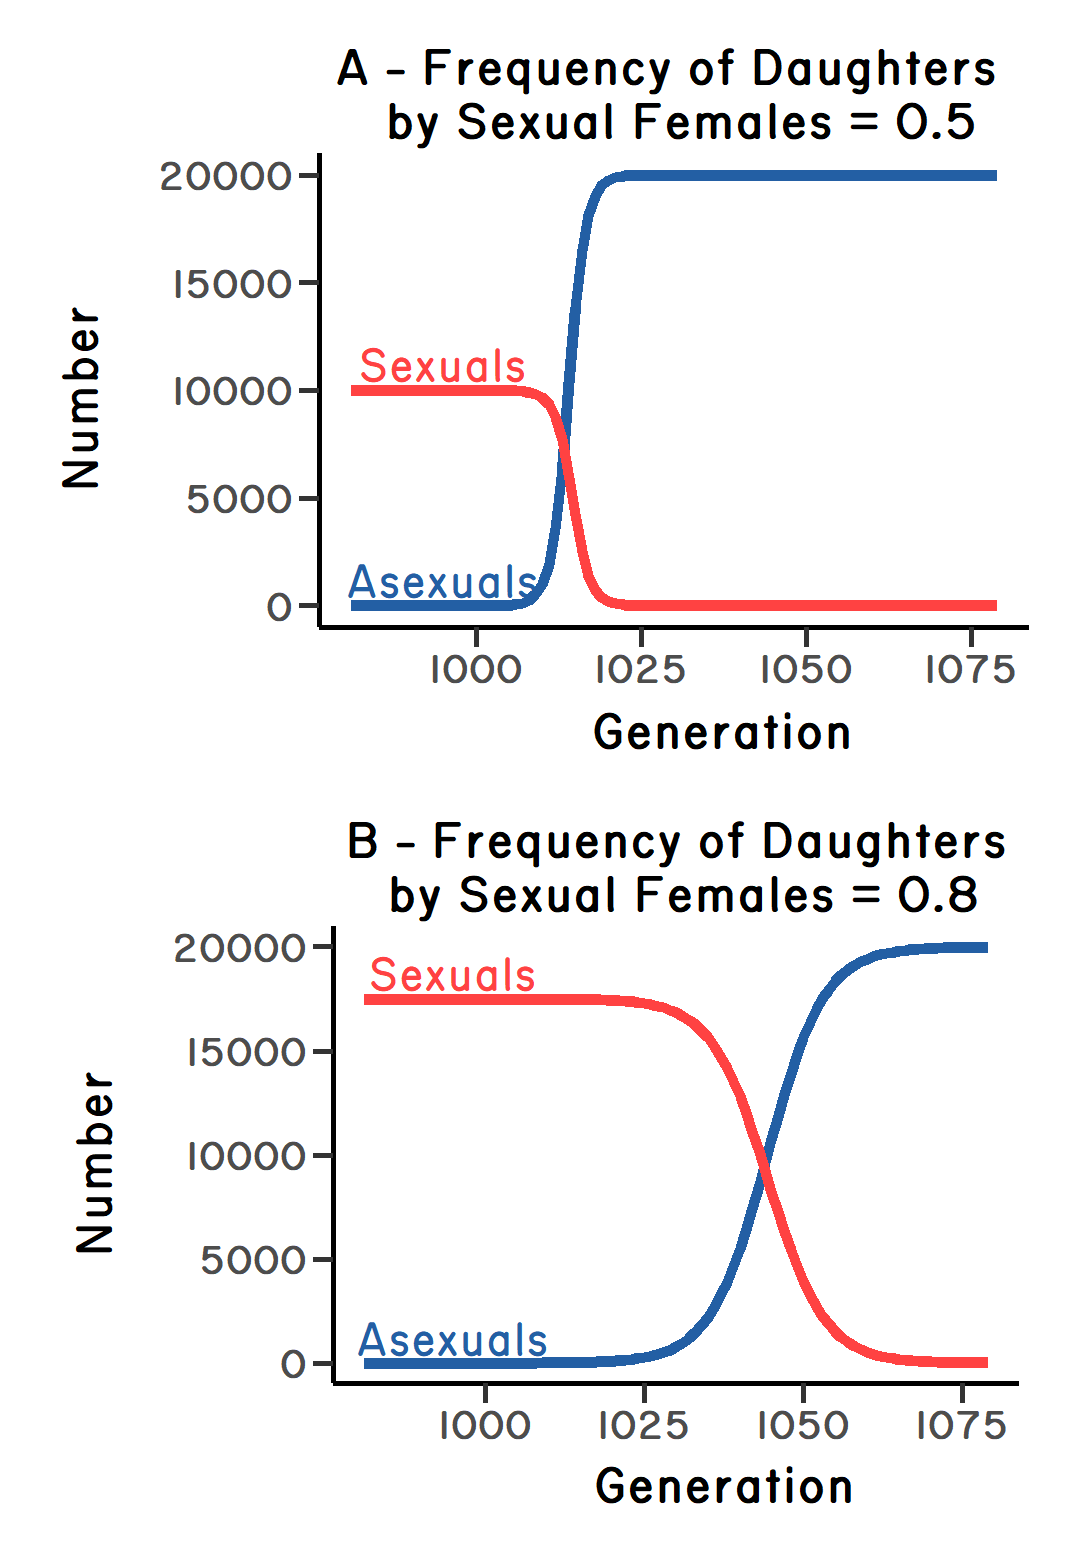
\includegraphics[width=0.55\textwidth,height=\textheight]{images/fig1-3_hr.png}

}

\caption[Clonal invasion dynamics]{\label{fig-1.2}Clonal invasion
dynamics. Results from a simulation study in which a single clonal
individual was introduced into a sexual population
(\citeproc{ref-lively2009a}{Lively 2009}). \textbf{A (top)}. Results for
a one-to-one sex ratio in the sexual population. Here the frequency of
daughters produced by sexual females was 1/2. The sexual population was
initiated at carrying capacity: \(K_{sex}\) = 10,000. A single
parthenogenetic female was introduced by the simulation at generation
1,000. Note that the asexual lineage replaces the sexual population in
about 25 generations, and that it reaches a higher carrying capacity
\(K_{asex}\) = 20,000. \textbf{B (bottom)}. Results for a female-biased
sexual population. Here the frequency of daughters produced by sexual
females was 0.8. The sexual population was initiated at carrying
capacity: \(K_{sex}\) = 17,500. As above, a single parthenogenetic
female was introduced into the population at generation 1,000. Note that
the asexual lineage replaces the sexual population, but it takes longer.
The simulation assumes annual reproduction and non-overlapping
generations. The data can also be explored in an
\href{https://connect.posit.iu.edu/clonal-invasion-dynamics/}{interactive
visualization}. We have made accessible
\href{https://raw.githubusercontent.com/IULibScholComm/through-the-looking-glass/main/rscripts/sim\%20for\%20fig\%201.2(ZMD).R}{the
R code for the static simulation} and
\href{https://raw.githubusercontent.com/IULibScholComm/through-the-looking-glass/main/rscripts/app.R}{the
R code for the interactive simulation}.}

\end{figure}%

\subsection{The cost of recombination}\label{the-cost-of-recombination}

There is another paradox of sexual reproduction known as the ``cost of
recombination.'' Here the competition is not between sexual and asexual
females, or between outcrossing and selfing alleles, but rather between
alleles that modify the rate of recombination. So instead of asking
``Why cross-fertilize?'' we can assume cross-fertilization and ask,
``Why is there excess crossing-over during meiosis?'' Here is the
paradox. If combinations of alleles at different loci are favored by
natural selection (because together they create high-fitness offspring),
then recombination would break these favorable allelic combinations
apart. So, it makes no obvious sense to recombine more than needed for
normal meiosis. Indeed, Lewontin (\citeproc{ref-lewontin1971a}{1971})
formally showed that ``the mean fitness of the population at equilibrium
is a maximum in the absence of recombination.''\footnote{Lewontin
  (\citeproc{ref-lewontin1971a}{1971}) was following up on Fisher's
  (\citeproc{ref-fisher1930a}{1930}) verbal suggestion that selection
  should act to reduce recombination. For example, Lewontin
  (\citeproc{ref-lewontin1971a}{1971}) writes, ``I will show \ldots{}
  that Fisher's conjecture is indeed correct.'' Importantly, in his last
  paragraph, Lewontin wonders why recombination rates are greater than
  zero, and he suggests that the answer ``must be sought in some more
  general long-term advantage for adaptation to a varying environment,
  or else to some mechanical necessity of recombination for the orderly
  distribution of chromosomes, as suggested by Darlington
  (\citeproc{ref-darlington1939a}{1939}).'' (See also
  \citeproc{ref-bell1982a}{Bell 1982}).} Hence, there are two
interrelated anomalies: cross-fertilization \emph{per se} and meiotic
recombination. Ideally, any theory that explains the persistence of
biparental sex could also solve the paradox of recombination. But this
need not be the case. They could have different solutions.

\subsection{Darwin's view}\label{darwins-view}

Even before the cost of males and meiosis were so dramatically revealed
by Williams and Maynard Smith, biologists were reckoning with the
anomaly of sex (\citeproc{ref-dagg2016a}{Dagg 2016}; reviews in
\citeproc{ref-meirmans2009a}{Meirmans 2009}). One of the earliest of
these biologists was Charles Darwin. After he published the \emph{Origin
of Species}, Darwin was doing hand-pollination experiments at Down House
on three species of a curious annual plant in the genus \emph{Primula}.
The plant is curious in that it has two morphs. One morph has a style
that extends beyond the anthers (the long-style morph), and the other
morph has anthers that extend beyond the style (the short-style morph).
Botanists refer to this condition as distyly (Figure~\ref{fig-1.3}).
Darwin (\citeproc{ref-darwin1862a}{1862}) found that crosses between the
different morphs of the same species resulted in a very successful
production of seeds, but crosses between unrelated individuals of the
same morph were dramatically less successful. In discussing these
results, Darwin speculated that the two morphs may have evolved to
ensure cross-fertilization: ``Whether or not the dimorphic condition of
the \emph{Primula} has any bearing on other points in natural history,
it is valuable as showing how nature strives, if I may so express
myself, to favour the sexual union of distinct individuals of the same
species.''

\begin{figure}

\centering{

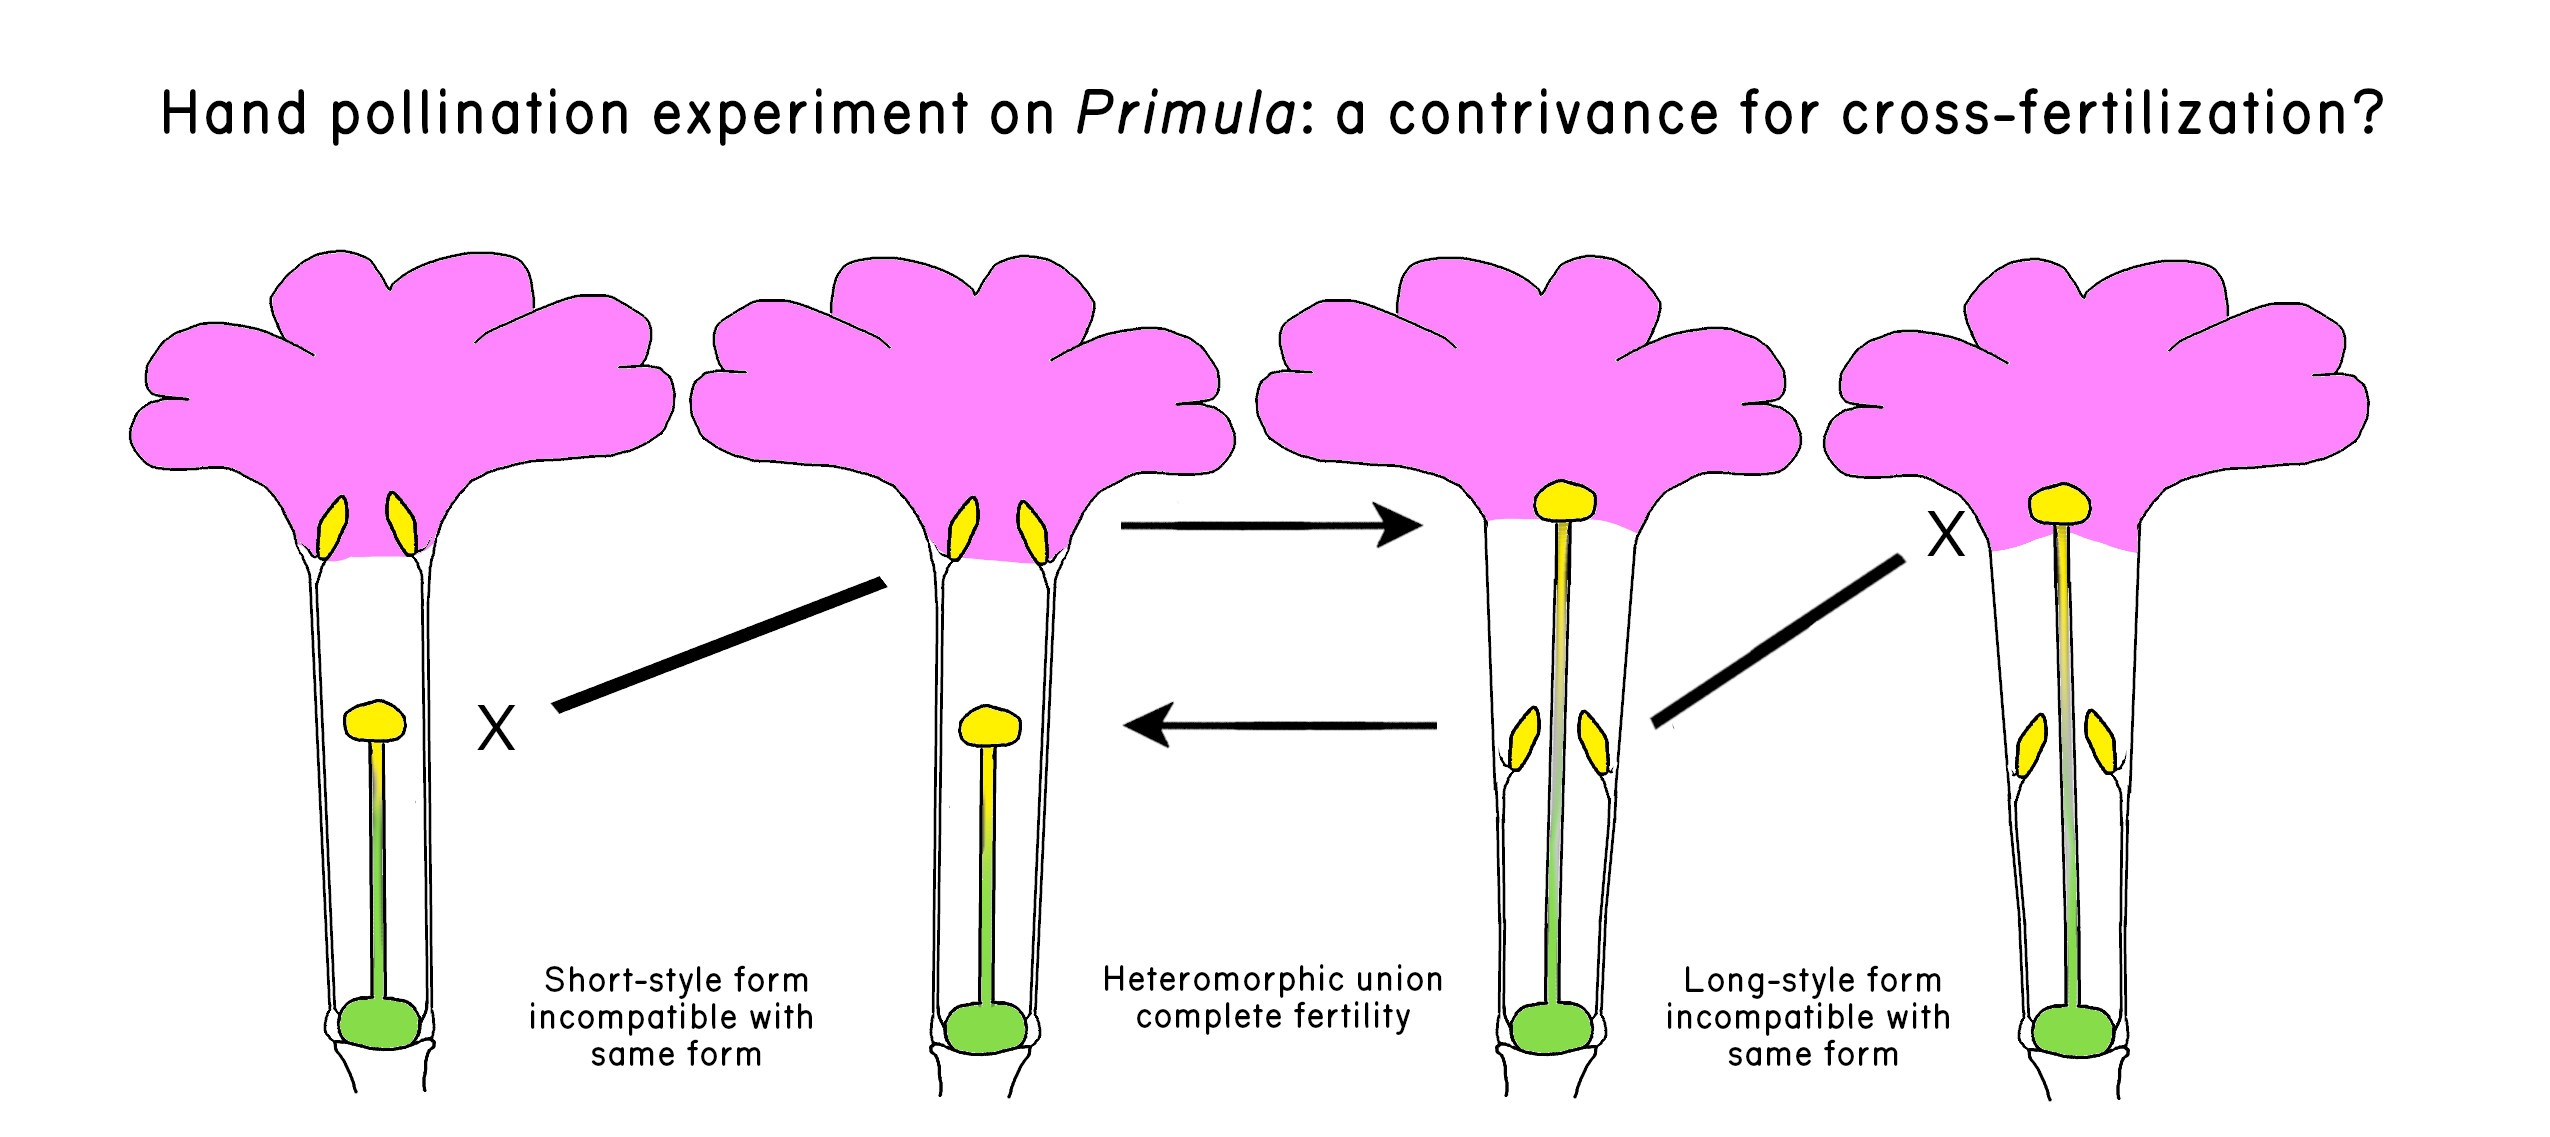
\includegraphics{images/fig1-4.jpg}

}

\caption[Two flower morphs (distyly) in
\emph{Primula}]{\label{fig-1.3}Two flower morphs (distyly) in
\emph{Primula}. Darwin found that the short-styled morph (left) is
incompatible with other short-style morphs and that the long-styled
morph (right) is incompatible with other long-style morphs. But the two
different morphs can cross-fertilize. The arrows show movement of pollen
from anthers to stigmas. The ``X'' indicates incompatibility. Redrawn
from Darwin (\citeproc{ref-darwin1862a}{1862}) by ZMD.}

\end{figure}%

Darwin then asks a killer question. Why should the union of elements
from distinct individuals be favored? Why, in fact, is there sex? ``Nor
do we know why nature should thus strive after the intercrossing of
distinct individuals. We do not even in the least know the final cause
of sexuality; why new beings should be produced by the union of the two
sexual elements, instead of by a process of parthenogenesis. The whole
subject is as yet hidden in darkness.'' Darwin's question shows that the
cross-fertilization is curious, even without considering the costs of
sex. It also shows how Darwin was drawn to anomalies on
theory.\footnote{For example, Darwin calls the evolution of sterile
  castes in social insects an ``insuperable difficulty'' for his theory
  of evolution by natural selection (pages 236-238 in
  \citeproc{ref-darwin1859a}{1859}).}

It is interesting to note that, in Darwin's quote above, he switches
from discussing mechanisms to prevent self-fertilization, such as
distyly, to discussing parthenogenesis. Self-fertilization is a sexual
process (involving the formation and fusion of gametes from the same
parent), while parthenogenesis is an asexual process that does not
generally involve meiosis and syngamy (review in
\citeproc{ref-bell1982a}{Bell 1982}). But parthenogenesis and
self-fertilization are conceptually related, as they are both
uniparental forms of reproduction. Hence, it makes sense that Darwin
would switch back and forth between these two different forms of
uniparental reproduction. Why cross-fertilize if either selfing or
parthenogenesis is an option?

There may be another reason why Darwin pivots to parthenogenesis. Just
prior to the publication of Darwin's (\citeproc{ref-darwin1862a}{1862})
paper on \emph{Primula}, Carl Theodor Ernst von Siebold
(\citeproc{ref-siebold1856a}{1856}) published his observations on the
successful development of adults from unfertilized eggs, which he called
``parthenogenesis'' (virgin birth). These were revolutionary
observations, which caught Darwin's attention. In a letter to his
mentor, J.S. Henslow, Darwin mentioned von Siebold's discovery as
follows: ``There is no greater mystery in the whole world, as it seems
to me, than the existence of sexes, -- more especially since the
discovery of Parthenogenesis'' (\citeproc{ref-darwin1860a}{Darwin
n.d.}).

However, the discovery of parthenogenesis was met with some
hostility.\footnote{The case has been made that Charles Bonnet had
  discovered asexual reproduction in aphids in 1740 (see
  \citeproc{ref-lawrence2009a}{Lawrence 2009}).} Consider, for example,
the following statement by Rudolf Wagner in his 1857 review of von
Siebold's book on parthenogenesis (as translated from the original
German by Churchill \citeproc{ref-churchill1979a}{1979}): ``I must
unfortunately say that one of the most unpleasant of facts,
{[}\emph{Parthenogenesis}{]} has been introduced into physiology, which
for the hope of so-called general laws of animal life-phenomena \emph{is
most distasteful}. It is impossible, considering the glorification of
our highly vaunted progress in the theoretical understanding of the life
processes, for it to be welcomed or particularly encouraged; and
sincerely speaking, I can be as little pleased about it as a physicist
would be if suddenly one or more exceptions to the law of gravitation
were discovered'' (Emphasis added).

Clearly, Wagner was not pleased with the discovery of asexual
reproduction, calling it unpleasant, unwelcome, and distasteful. By
contrast, Darwin did not find the idea to be distasteful in any way. He
wondered instead why it was not more common. For example, Darwin
(\citeproc{ref-darwin1868a}{1868}) wrote, ``Parthenogenesis is no longer
wonderful; in fact, the wonder is that it should not oftener
occur.''\footnote{I suspect that Darwin uses the phrase ``no longer
  wonderful'' to mean ``no longer astonishing.'' See
  \href{https://www.merriam-webster.com/words-at-play/wonderful-word-history-evolution}{``How
  `Wonderful' Lost Its Sense of Wonder.''}}

Over 100 years later, W. D. Hamilton
(\citeproc{ref-hamilton1975a}{1975b}) was also pondering the evolution
of outcrossing, and he wrote something conceptually similar:
``{[}c{]}omplete inbreeding abandons the obviously important advantages
of sexual reproduction, whatever these are.'' Whatever these are! The
advantages of outcrossing were obviously important because
cross-fertilization is so dominant. But the source of these advantages
was not clear. At about the same time, Maynard Smith
(\citeproc{ref-maynard1976a}{1976}) mused, ``One gets the feeling that
some essential feature of the situation has been overlooked.''

I now think that John Maynard Smith was correct. An essential feature
had indeed been overlooked: parasites.

\section{Summary}\label{summary}

\begin{enumerate}
\def\labelenumi{\arabic{enumi}.}
\tightlist
\item
  Obligate sexual reproduction is subject to invasion and replacement by
  all-female asexual lineages that do not pay the cost of males.
\item
  Obligate outcrossing in simultaneous hermaphrodites is subject to
  invasion and replacement by self-fertilization unless inbreeding
  depression is severe.
\item
  The exchange of DNA between different parental chromosomes
  (recombination) is similarly paradoxical.
\item
  Why then are recombination and cross-fertilization so common?
\end{enumerate}

\section{Appendix: Maynard Smith's Model}\label{sec-app-1}

John Maynard Smith's (\citeproc{ref-maynard1978a}{1978}) model,
reproduced here, shows the cost of producing males.\footnote{I use
  slightly different variable names and try to simplify JMS's original
  model.} Let \(N_{asex}\) be the number of asexual females at time one,
while \(N_{sex}\) gives the total number of sexual individuals (males
plus females) at time one. Let \(B_{asex}\) give the number of offspring
produced by asexual females, and \(S_{asex}\) gives the survival
probability of asexual offspring to maturity. The number of surviving
asexual offspring is then \(= B_{asex}S_{asex}\). Similarly, let
\(B_{sex}\) be the number offspring produced by sexual females, and let
\(S_{sex}\) give the survival probability of sexually produced
offspring. Maynard Smith assumed that all individuals reproduce once and
then die. Let \(r\) be the frequency of females in the sexual
population. The number of asexuals and sexuals at time two can then be
calculated as in the table below. (Note, we do not assume that the
population is at carrying capacity).

\begin{longtable}[]{@{}
  >{\centering\arraybackslash}p{(\columnwidth - 4\tabcolsep) * \real{0.1465}}
  >{\centering\arraybackslash}p{(\columnwidth - 4\tabcolsep) * \real{0.2611}}
  >{\centering\arraybackslash}p{(\columnwidth - 4\tabcolsep) * \real{0.5924}}@{}}
\caption{Appendix: Maynard Smith's Model}\label{tbl-t1t2}\tabularnewline
\toprule\noalign{}
\begin{minipage}[b]{\linewidth}\centering
\end{minipage} & \begin{minipage}[b]{\linewidth}\centering
\textbf{Time One}
\end{minipage} & \begin{minipage}[b]{\linewidth}\centering
\textbf{Time Two}
\end{minipage} \\
\midrule\noalign{}
\endfirsthead
\toprule\noalign{}
\begin{minipage}[b]{\linewidth}\centering
\end{minipage} & \begin{minipage}[b]{\linewidth}\centering
\textbf{Time One}
\end{minipage} & \begin{minipage}[b]{\linewidth}\centering
\textbf{Time Two}
\end{minipage} \\
\midrule\noalign{}
\endhead
\bottomrule\noalign{}
\endlastfoot
\textbf{N. of asexuals} & \(N_{asex}\) &
\(N_{asex}(S_{asex}B_{asex})\) \\
\textbf{N. of sexuals} & \(N_{sex}\) & \(rN_{sex}(S_{sex}B_{sex})\) \\
\textbf{Freq. of asexuals} & \(\frac{N_{asex}}{N_{asex} + N_{sex}}\) &
\(\frac{N_{asex}(S_{asex}B_{asex})}{N_{asex}(S_{asex}B_{asex})+rN_{sex}(S_{sex}B_{sex})}\) \\
\end{longtable}

The fold increase in frequency of asexuals, \(F\), is the ratio of the
frequency of asexuals at time two divided by the frequency of asexuals
at time one giving
\[F = \frac{N_{asex}(S_{asex}B_{asex})}{N_{asex}(S_{asex}B_{asex}) + r(N_{sex}S_{sex}B_{sex})}/\frac{N_{asex}}{N_{asex} + N_{sex}}.\]
Under the all-else-equal assumption, \(S_{asex} = S_{sex}\) and
\(B_{asex} = B_{sex}\), giving
\[F = \frac{N_{asex}}{N_{asex} + rN_{sex}}/\frac{N_{asex}}{N_{asex} + N_{sex}}.\]
Assuming that there is a single asexual female at time one, we get
\[F = \frac{1}{1 + rN_{sex}}/\frac{1}{1 + N_{sex}} = \frac{1 + N_{sex}}{1 + rN_{sex}}.\]
If \(N_{sex}\) is very large, the solution reduces to \(F \approx 1/r\).
Hence, the fold increase in the frequency of asexuals, \(F\), is
inversely related to the frequency of females \((r)\) in the sexual
subpopulation. Assuming a one-to-one sex ratio, \(r = 0.5\). Hence, for
an equal sex ratio, the increase in asexuals is \(\approx\) two-fold.
This result gives the two-fold cost of males. Assuming
``all-else-equal'' a clone will double when rare when introduced into a
large sexual population.

\bookmarksetup{startatroot}

\chapter{The Ecological Hypotheses}\label{sec-eco-hyp}

\begin{center}
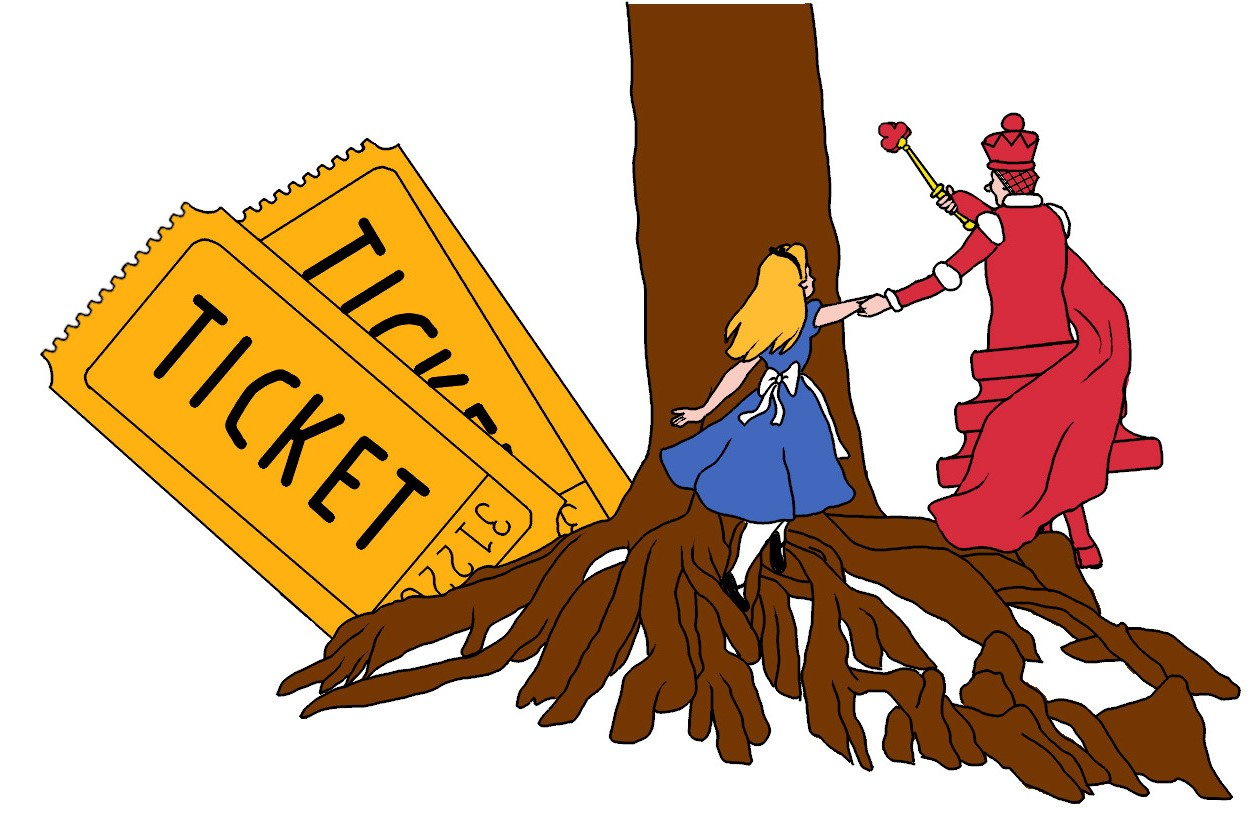
\includegraphics[width=0.7\textwidth,height=\textheight]{images/fig2-1.jpeg}
\end{center}

The sex/recombination (``sex/rec'') anomaly has attracted some of the
best theoretical biologists over the last 50 years leading to at least
two dozen hypotheses to explain selection for recombination and/or the
persistence of obligate sexual reproduction in natural populations
(\citeproc{ref-kondrashov1993a}{Kondrashov 1993}). In what follows, I
first focus on the ecological hypotheses. The ideas underlying these
hypotheses provide a handle for understanding some of the foundational
concepts in evolutionary ecology.

\section{The Lottery Model}\label{the-lottery-model}

As part of his book on the evolution of sex, Williams
(\citeproc{ref-williams1975a}{1975}) suggests that sex could be favored
in fluctuating abiotic environments. The idea is intuitive:
cross-fertilization generates variation among offspring. Hence, in
fluctuating environments, sex could increase the probability that some
offspring might survive. Williams likens the idea to a unique kind of
lottery. For example, he writes, ``Suppose you were offered this choice
in a lottery: either you could have several different tickets, or you
could have the same number of copies of the same ticket'' (p.~15). If
you choose \emph{N} copies of the same ticket (asex) and your ticket
wins, you get \emph{N} times the reward. If you choose \emph{N}
different tickets (sex), you increase the probability of winning
something, but the reward is smaller. Williams refers to the idea as the
aphid-rotifer model, but the idea has since come to be known as the
Lottery Model (following \citeproc{ref-bell1982a}{Bell 1982}), which is
a more descriptive phrase.\footnote{See Bell
  (\citeproc{ref-bell1982a}{1982}) for a deeper historical view of the
  Lottery Model, which involves contributions by Maynard Smith and
  others, including Williams. I have tried to distill it down to a
  simple bet-hedging model here. The original formulation is more
  complex.}

In my evolution course, I ask a form of Williams' question but with a
slight twist:

\begin{quote}
If you had a garden, upon which your descendants will depend for many
generations to come, would you

\begin{enumerate}
\def\labelenumi{\arabic{enumi}.}
\tightlist
\item
  plant a genetically variable crop, or
\item
  a monoculture with a two-fold higher yield?
\end{enumerate}

Keep in mind that your descendants will follow your choice.
\end{quote}

Often the students rightfully want some clarification. They ask, for
example, ``Can we use pesticides?'' But every time, most students choose
the variable crop. I remind them that selecting the variable crop will
reduce their yield by one half. They don't budge. I re-ask the question,
doubling the relative yield for the monoculture from two-fold to
four-fold. Then to 10-fold. Occasionally, one of the more risk-prone
students will select the 10-fold higher yield, but most do not budge.
They want genetic variation. I ask them why. Invariably, they say that
the environment is going to change. They want to hedge their bets
against an uncertain future.

Indeed, Williams' Lottery Model is about bet hedging. The gist of bet
hedging in evolutionary theory is that selection can act to reduce the
variance in reproductive success over time, even if it also reduces the
arithmetic mean across years (review in
\citeproc{ref-philippi1989a}{Philippi \& Seger 1989}). Suppose, for
example, that we have data for both a monoculture and a genetically
variable polyculture (Table~\ref{tbl-bh}). Let's assume that the
variation in yield is driven by annual variation in abiotic factors such
as temperature or precipitation. The effect of planting a polyculture
(bet-hedging) can be estimated from the geometric mean, which
incorporates the variation in yield over time.

In this example, we find that the monoculture has an arithmetic mean of
240, while the polyculture has an arithmetic mean of only 220. So, I
might be inclined to plant the monoculture. However, the among-year
variance is very high for the monoculture (relative to the polyculture),
driven in large part by the low yields in years 4 and 5. By contrast,
the geometric mean for the monoculture is 184, while the geometric mean
for the polyculture is 219. Based on this, I might be inclined to plant
the polyculture, as it reduces the cost of very low yield in bad years.
I think the students see this intuitively. Over the long term, it is
better to be risk-averse and plant the genetically variable polyculture.
What if, for example, the monoculture produced no food in the last year?
The geometric mean would be zero. That would be catastrophic.

\begin{longtable}[]{@{}
  >{\raggedright\arraybackslash}p{(\columnwidth - 4\tabcolsep) * \real{0.3421}}
  >{\raggedright\arraybackslash}p{(\columnwidth - 4\tabcolsep) * \real{0.3158}}
  >{\raggedright\arraybackslash}p{(\columnwidth - 4\tabcolsep) * \real{0.3158}}@{}}
\caption{Bet Hedging. The entries show annual yields (in arbitrary
units) over five years for a monoculture and a
polyculture.}\label{tbl-bh}\tabularnewline
\toprule\noalign{}
\begin{minipage}[b]{\linewidth}\raggedright
Year
\end{minipage} & \begin{minipage}[b]{\linewidth}\raggedright
Monoculture
\end{minipage} & \begin{minipage}[b]{\linewidth}\raggedright
Polyculture
\end{minipage} \\
\midrule\noalign{}
\endfirsthead
\toprule\noalign{}
\begin{minipage}[b]{\linewidth}\raggedright
Year
\end{minipage} & \begin{minipage}[b]{\linewidth}\raggedright
Monoculture
\end{minipage} & \begin{minipage}[b]{\linewidth}\raggedright
Polyculture
\end{minipage} \\
\midrule\noalign{}
\endhead
\bottomrule\noalign{}
\endlastfoot
1 & 350 & 250 \\
2 & 400 & 250 \\
3 & 300 & 200 \\
4 & 100 & 200 \\
5 & 50 & 200 \\
~ & ~ & ~ \\
Arithmetic mean & 240 & 220 \\
Variance\footnote{The variance in \(x\) is equal to the average of the
  squared deviations from the mean:
  \(var(x) = \frac{1}{N}\sum_{i = 1}^{N}{(x_{i} - \overline{x})^{2}}\).}
& 19400 & 600 \\
Geometric mean (GM)\footnote{The geometric mean is the \(N^{th}\) root
  of the product of \(N\) observations. Compared to the arithmetic mean,
  the geometric mean gives more weight to small values.} & 184 & 219 \\
Approximate GM & 200 & 219 \\
\end{longtable}

The effect of variance on the geometric mean (GM) can be seen by an
approximation (\citeproc{ref-stearns2000a}{Stearns
2000}):\[\text{GM} \approx \overline{x} - \frac{\text{var}(x)}{2\overline{x}}\]
where \(\overline{x}\) is the mean, and var(\(x\)) is the variance in
\(x\). Note that the approximation is equal to the arithmetic mean when
the variance in \(x\) is zero. Note too that the geometric mean
increases as the variance in \(x\) decreases. So, if selection operates
to reduce the among-year variance in fitness, the outcome of selection
will be reflected by an increase in the geometric mean. In general,
evolutionary biologists use the geometric mean (rather than the
arithmetic mean) to measure fitness over time.\footnote{The bet-hedging
  idea dates to Daniel Bernoulli, a mathematical physicist, writing in
  1738. Steve Stearns (\citeproc{ref-stearns2000a}{2000}) provides an
  important, fascinating review of how evolutionary biologists
  (beginning with \citeproc{ref-cohen1966a}{Cohen 1966}) and economists
  have borrowed from Bernoulli's conceptual framework.}

Can sex be favored in variable environments as a bet-hedging strategy?
It seems like a very sensible idea provided that the production of
genetically variable progeny reduces the among-year variance in
offspring survival. But remember, under a two-fold cost of sex, asexuals
can replace large populations of sexuals in tens of generations (see
Chapter~\ref{sec-why-sex}). So, if the Lottery Model is correct,
significant environmental change must occur very rapidly. The many
thousands of years between ice ages, for example, would be too long.

\section{The Tangled Bank / Frozen Niche-Variation
Model}\label{sec-niche}

Roughly speaking, the Lottery Model concerns the value of producing
diverse offspring in a temporally variable abiotic environment. A
different kind of model instead concerns the role of competition for
different resource types that vary in space. Let us first consider the
Frozen Niche-Variation Hypothesis of Robert Vrijenhoek. The key idea is
that the clonal derivatives of sexual ancestors ``freeze'' some of the
genetic variation in the sexual population. This frozen genotype then
determines the resource niche of the clone. It seems reasonable to
assume that the niche width of a single clone would be relatively narrow
compared to the niche width of the genetically diverse sexual
population. So, under this idea, a clone could invade a sexual
population and perhaps displace it from one of its many niches. But a
single clone could not completely replace the sexual population
(\citeproc{ref-vrijenhoek1979a}{Vrijenhoek 1979}). This kind of process
could explain those situations in which sexual and asexual females
coexist, which was a major advance.\footnote{Vrijenhoek studied the
  coexistence of sexual fish with multiple clonal genotypes of asexual
  congeners in natural populations. He mainly envisioned the Frozen
  Niche Hypothesis as a model to explain the coexistence of multiple
  clones, but it can also explain the coexistence of sexual and asexual
  modes of reproduction if clonal diversity is low, and the clones do
  not compete strongly. See, for example pages 112-113 in Vrijenhoek and
  Parker (\citeproc{ref-vrijenhoek2009a}{2009}): ``The Frozen Niche
  Variation Model (\citeproc{ref-vrijenhoek1978a}{Vrijenhoek 1978},
  \citeproc{ref-vrijenhoek1979a}{1979}) was directly stimulated by
  Roughgarden's (\citeproc{ref-roughgarden1972a}{1972}) ideas and a need
  to explain the stable coexistence of \emph{Poeciliopsis} fish clones
  in spatially heterogeneous desert streams
  (\citeproc{ref-vrijenhoek1978a}{Vrijenhoek 1978}).''}

A conceptually similar model was independently developed by Graham Bell
(\citeproc{ref-bell1982a}{1982}): the Tangled Bank Hypothesis. Bell
nabbed the name from the last paragraph of the \emph{Origin of Species},
in which Darwin imagines life as an ``entangled bank'' of species
interacting in a complex network. The core of the idea can be traced
back to Howard Levene's (\citeproc{ref-levene1953a}{1953}) pioneering
model, which showed that polymorphism could be maintained in a spatially
heterogeneous environment provided that different genotypes specialize
on different resources. Levene's model was a major advance, as it showed
that genetic diversity could be maintained without heterozygote
advantage (Section~\ref{sec-app-2}). This was also one of the first
models to fuse population genetics with ecology. But how does multiple
niche polymorphism apply to sex? The idea is that if selection results
in polymorphism, then a genetically diverse sexual population might be
resistant to replacement by a clonal lineage that specializes on only
one of the available resource types (as also in the Frozen
Niche-Variation Model).

Here is how I pose the Tangled Bank idea to my undergraduate students. I
start by giving them a choice between two hypothetical resources, which
occur in different parts of the room. One is pizza, the other is
broccoli. They all choose pizza. The problem, of course, is that the
per-person value of the pizza resource declines as the pizza-eating
population grows. At some point, there will be an advantage to
specializing on broccoli. This could lead to a polymorphic population
composed of obligate pizza eaters and obligate broccoli eaters, where
(at equilibrium) the value of both resources is the same. Hence,
selection for or against a particular strategy depends on the frequency
of that strategy in the population. Perhaps this kind of
``frequency-dependent selection'' could favor sexual reproduction as a
way to diversify offspring in environments where different resource
types are patchily distributed in space. This reasoning forms the
essence of the Tangled Bank Hypothesis.

One especially interesting aspect of the Tangled Bank Model is that the
strength of frequency-dependent selection depends on population density.
For example, there would be no selection to utilize the resource of
lower value (broccoli) if there were no competition for pizza. This kind
of selection, where the advantage to being rare depends on population
density, is sometimes referred to as ``soft'' selection
(\citeproc{ref-wallace1975a}{Wallace 1975}).\footnote{Soft selection in
  theoretical population genetics can also mean that the contribution of
  offspring from different demes in a metapopulation is unrelated to
  differences in mean fitness among demes.} In other words, soft
selection is selection that is both frequency-dependent and
density-dependent. This idea contrasts nicely with the Lottery Model,
where selection is both frequency- and density-independent, which is
called ``hard'' selection. For our purposes, we can use Wallace's
terminology to conceptually separate the Tangled Bank Hypothesis from
the Lottery Model Figure~\ref{fig-2-2}.

\begin{figure}

\centering{

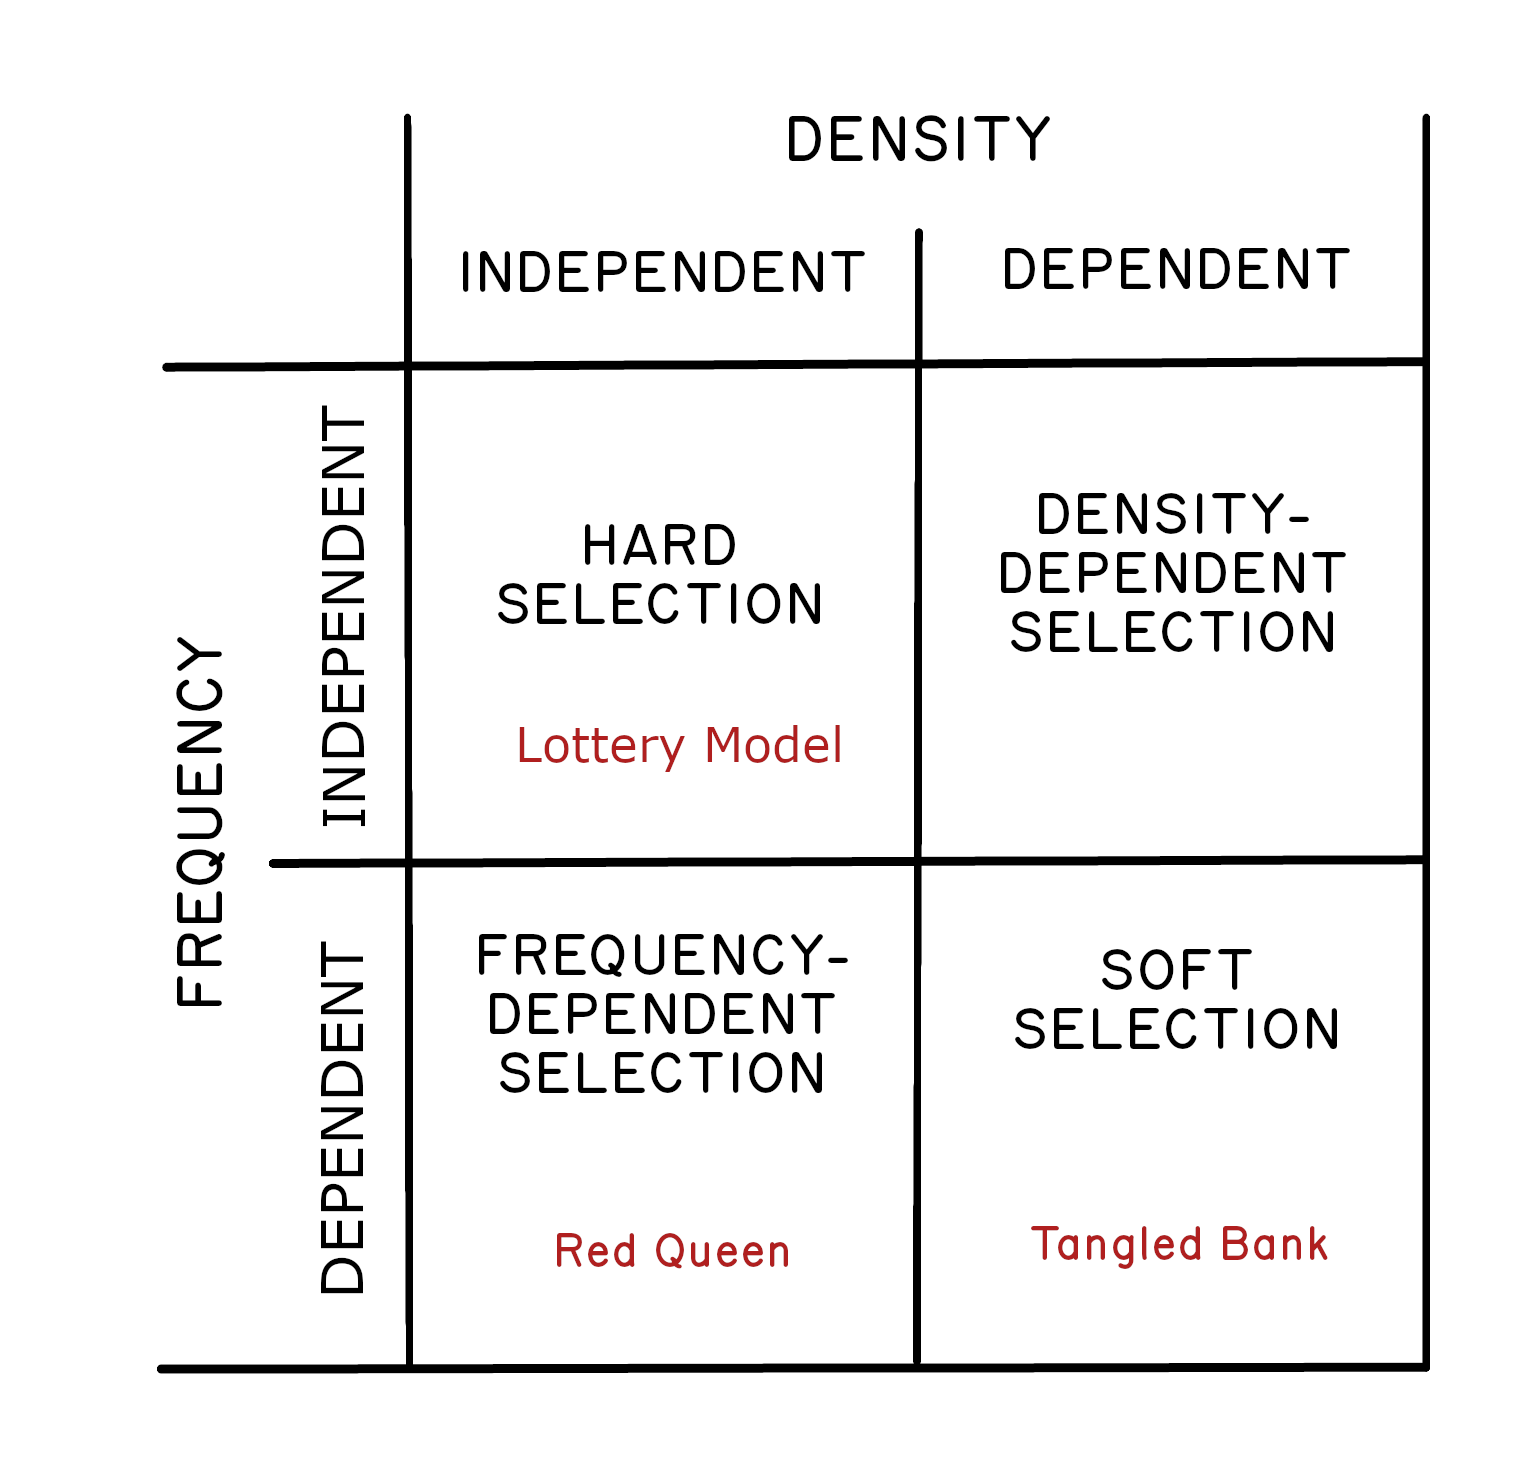
\includegraphics[width=0.6\textwidth,height=\textheight]{images/fig2-2_hr.png}

}

\caption[Partitioning the ecological hypotheses for the maintenance of
obligate sexual reproduction]{\label{fig-2-2}Partitioning the ecological
hypotheses for the maintenance of obligate sexual reproduction. The
figure is redrawn from Wallace (\citeproc{ref-wallace1975a}{1975}). The
inserted red text shows how the ecological hypotheses fit into Wallace's
matrix for density-dependent selection versus frequency-dependent
selection. The Lottery Model relies on hard selection in temporally
variable environments. The Tangled Bank relies on soft selection in
spatially variable environments. The Red Queen relies on
frequency-dependent selection generated by coevolving antagonistic
species.}

\end{figure}%

We can think of the contrast like this. Under the Lottery Model, changes
in the environment will select against certain genotypes independent of
whether they are common or rare. Selection seems unconditional (hard).
Under the Tangled Bank, selection is always conditional (soft); there is
an advantage to having a rare genotype, but this advantage only accrues
under strong competition (high density). Soft selection may not be
exactly the best possible phrase, but it contrasts nicely with hard
selection.\footnote{Wallace (\citeproc{ref-wallace1975a}{1975}) explains
  that the source of the terms ``soft'' and ``hard'' stem from financial
  discussions of soft currencies versus hard currencies in monetary
  exchanges. Soft currencies only have value within their home country.
  In contrast, hard currencies can be exchanged overseas for currencies
  with similar buying power.}

Two caveats are worth mentioning with respect to soft selection and the
Tangled Bank Hypothesis. One is that polymorphism is only stable under a
narrow range of patch-types frequencies. In addition, strong tradeoffs
are required for the cost and benefits for morphs occupying different
patches (\citeproc{ref-lively1986a}{Lively 1986a};
\citeproc{ref-maynard1980a}{Maynard Smith \& Hoekstra 1980}) (see also
Section~\ref{sec-app-3}). The second caveat is that repeated mutation to
asexual reproduction could lead to the accumulation of clonal diversity
over time. Once all the niches are occupied by different specialized
clones, there would be no advantage to sex. A diverse clonal population
could then replace the sexual population (\citeproc{ref-bell1982a}{Bell
1982}; \citeproc{ref-vrijenhoek2009a}{Vrijenhoek \& Parker 2009}). This
second caveat applies, in general, to any model of sex that relies on
frequency-dependent selection. But the ideas could work if mutations to
asex are rare. And, as I mentioned, sexuals and asexuals are known to
coexist in some populations, which is consistent with the Tangled Bank
and Frozen Niche-Variation Hypotheses
(\citeproc{ref-vrijenhoek2009a}{Vrijenhoek \& Parker 2009}).
Coexistence, however, is also compatible with the Red Queen hypothesis,
which we will now consider.

\section{The Red Queen Hypothesis}\label{the-red-queen-hypothesis}

The Red Queen Hypothesis is like the Lottery Model in that it focusses
on environmental change over time. However, under the Red Queen idea,
the change is mediated by changes in coevolving biological antagonists
such as parasites, rather than changes in the abiotic
environments.\footnote{I use ``parasite'' here in the ecological sense
  to include any organism that lives in, or on, its host, provided it
  reduces the survivorship and/or fecundity of its host. As such, the
  term includes both macroparasites (such as worms) and microparasites
  (such as protozoans, bacteria, and viruses).} The distinction is
important, as we will see.

It may be helpful to revisit Figure~\ref{fig-1.2}, which shows the
replacement of a sexual population by a clonal lineage within 25
generations. In this example, the clone is a single genotype, while the
sexual population is composed of multiple recombining genotypes, only
one of which is shared with the clone. Clearly, as the clone spreads,
its genotype would become the most common in the host population. Now
suppose that the host population is coevolving with a parasite
population, which is composed of multiple strains. Assuming random
contact between hosts and parasites, the parasite strain that could
infect the most common host genotype would have a selective advantage
over parasite strains that could only infect rare host genotypes. Let's
call this more successful parasite strain ``strain \textbf{A}.'' What
would happen? It should be easy to see that strain \textbf{A} would
increase in frequency. The parasite population would evolve.

Now, what if the parasite dramatically reduces the reproductive success
of infected hosts? We might expect that, as the parasite evolves to
infect the most-common host genotype, the reproductive advantage of the
host clone is eroded. Moreover, if the parasite is \emph{common and
sufficiently virulent}, evolution by the parasite could prevent the
clone from eliminating the sexual population. Under this scenario, there
are at least two possible outcomes. One is that the sexuals and asexuals
come to exist in stable frequencies, where the lost fecundity of the
clone due to infection is equal to the cost of males, meaning that the
mean fitnesses of sexuals and asexuals are equal. On the other hand, if
the parasite is highly virulent, the frequencies of sexuals and asexuals
can oscillate over time (Figure~\ref{fig-2-3} A). Under this second
scenario, the new clone initially increases, but it is driven down
sharply by infection (Figure~\ref{fig-2-3} B). Then, once the clone
becomes very rare, it should become less infected than observed in the
sexual population (Figure~\ref{fig-2-3} B). During this period, there is
parasite-mediated selection against sex. Hence, the clone increases in
frequency (Figure~\ref{fig-2-3} A), only to be driven down again by
parasites after it becomes common (Figure~\ref{fig-2-3} B). Another
cycle begins. \textbf{The key point is that parasites do not select
against clonal reproduction per se; they only select against common
genotypes.} But selection against common host genotypes might be
sufficient to prevent fixation of a clone in the short term.

\begin{figure}

\centering{

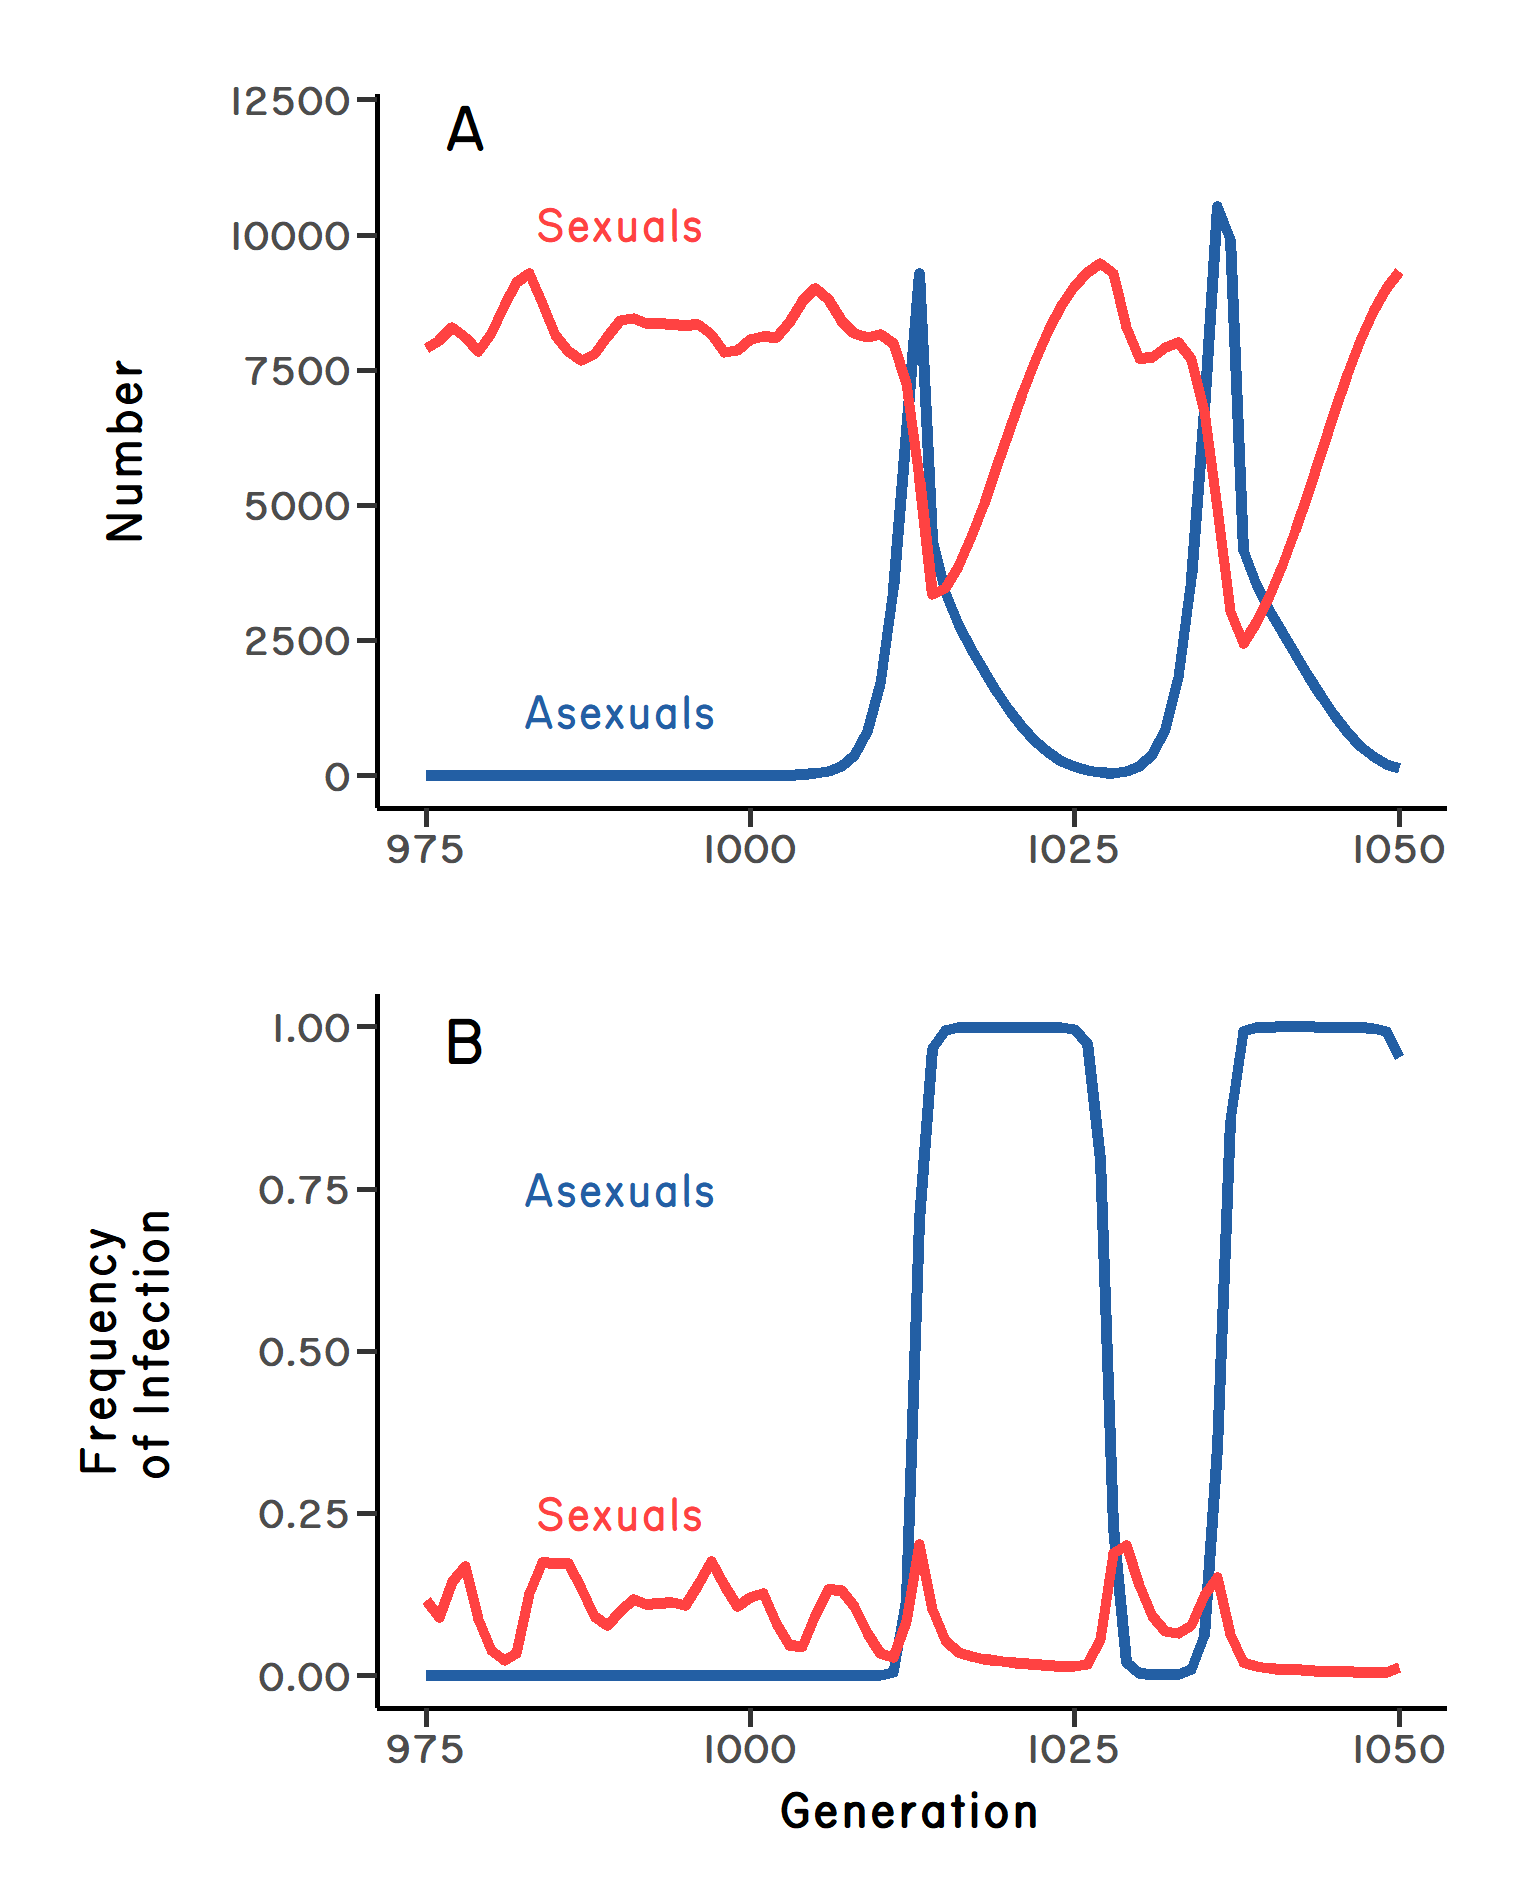
\includegraphics[width=0.65\textwidth,height=\textheight]{images/fig2-3_hr.png}

}

\caption[Simulation models showing that coevolving parasites can prevent
the fixation of asexuals in the short term]{\label{fig-2-3}Simulation
models showing that coevolving parasites can prevent the fixation of
asexuals in the short term. \textbf{A.} The number of sexual and asexual
individuals over time. \textbf{B.} The frequency of infection in sexual
and asexual individuals over time. The simulation introduces a single
clonal genotype into a sexual population at carrying capacity. After the
clone becomes common (\textbf{A}) the parasites evolve to ``target'' it
for infection (\textbf{B}). Note that after the parasites have driven
the clone's frequency down, the asexuals are less infected than the
sexuals. Simulation model based on Lively
(\citeproc{ref-lively2009a}{2009}), which treats parasite virulence as a
positive function of host density.}

\end{figure}%

This scenario of fluctuating selection for and against sex is just a
special case of the more general idea that parasites will select against
common genotypes within a diverse, sexual host population. As a rare
host genotype becomes common, the parasites genotype that can infect it
will be favored by natural selection. If the parasite is virulent
(meaning that infection reduces host fitness), the targeted host
genotype will decline in frequency, and a new host genotype will begin
to increase in frequency. Under this logic, host-parasite coevolution
will lead to the oscillation of genotypes in both the host and the
parasite populations (Figure~\ref{fig-2-4}). These oscillations are now
called Red Queen dynamics. Red Queen dynamics can lead to the
maintenance of genetic polymorphism in sexual populations, and possibly
protect sexual reproduction from replacement by asexual lineages. In
addition, Red Queen dynamics could also favor recombination within a
sexual population (\citeproc{ref-peters1999a}{Peters \& Lively 1999},
\citeproc{ref-peters2007a}{2007}; \citeproc{ref-salathe2008a}{Salathe
\emph{et al.} 2008}; \citeproc{ref-schmid-hempel2002a}{Schmid-Hempel \&
Jokela 2002}). These related ideas are now called the Red Queen
Hypothesis (following \citeproc{ref-bell1982a}{Bell 1982}).

\begin{figure}

\centering{

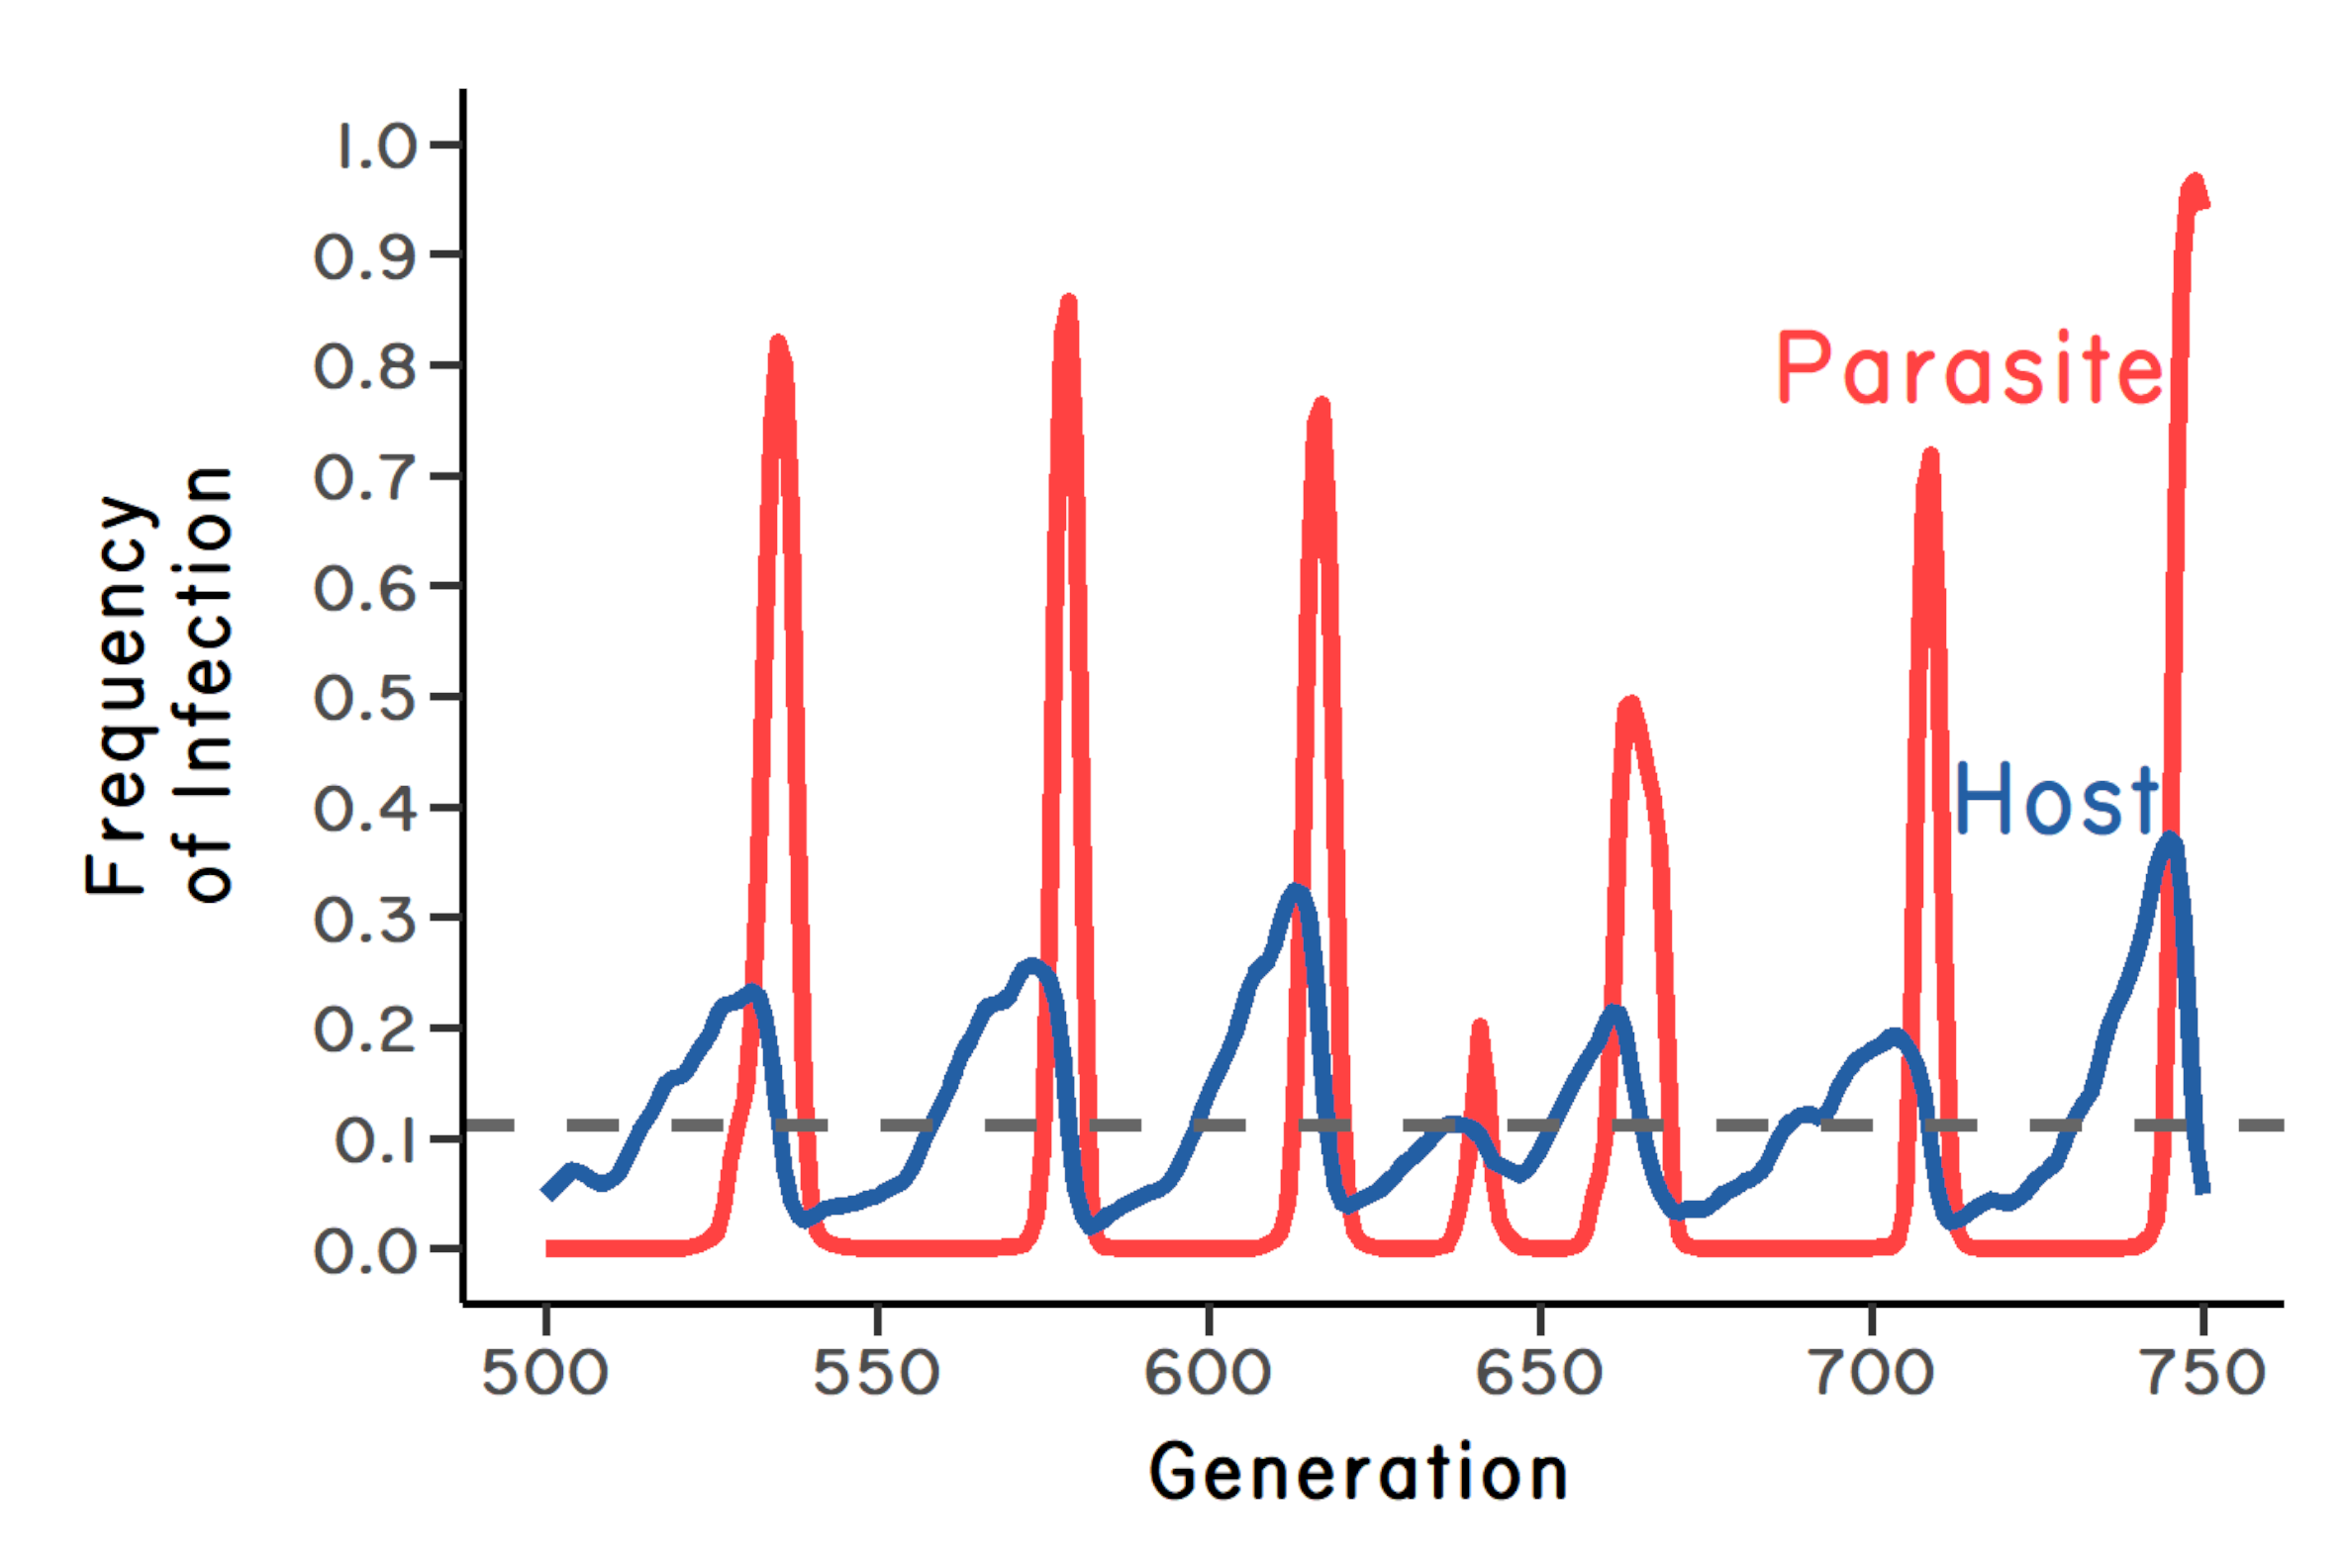
\includegraphics[width=0.65\textwidth,height=\textheight]{images/fig2-4_hr.png}

}

\caption[Red Queen dynamics]{\label{fig-2-4}Red Queen dynamics. The
frequency of a single host genotype is shown along with the frequency of
the only parasite genotype that can infect it. Note that the parasite
tracks the host with a time lag. Results were extracted from a
simulation of a sexual host population with nine possible genotypes
coevolving with an asexual parasite with nine matching genotypes
(\citeproc{ref-lively2009a}{Lively 2009}). The dashed line shows the
average genotype frequency for hosts and parasites.}

\end{figure}%

\subsection{An intersection of science and
literature}\label{an-intersection-of-science-and-literature}

The name for the Red Queen Hypothesis comes from \emph{Through the
Looking Glass} (\citeproc{ref-carroll1872a}{Carroll 1872}). Here are the
relevant bits of the story. After Alice goes through the looking glass
(a mirror), she decides to follow a straight path to the top of a hill.
But, in following the path, she ends up at her starting point. Talking
to herself, she remarks, ``But how curiously it twists! It's more like a
corkscrew than a path.'' Repeated attempts were unsuccessful. In
frustration, Alice addresses a tiger lily amongst a patch of flowers,
``I wish you could talk!'' The lily informs Alice that all the flowers
can talk. The stunned Alice then begins a conversation with the flowers
before finally asking, ``Are there any more people in the garden besides
me?'' The rose answers ``Yes, there is someone like you.'' Alice sets
out to follow this person (the Red Queen), but she quickly loses sight
of her, and ends up back at her original starting point. Flustered,
Alice decides to follow the advice of the rose: ``\emph{I} should advise
you to walk the other way.'' Alice then quickly finds the Red Queen.

Now it gets especially interesting. Alice mentions to the Red Queen that
she would like to ``find my way to the top of that hill.'' The Red Queen
replies, ``\emph{I} could show you hills, in comparison with which you'd
call that a valley.'' Alice protests: ``a hill \emph{ca'n't} be a
valley.\ldots{} That would be nonsense.'' This exchange between Alice
and the Red Queen now seems prophetic, because, under
frequency-dependent selection, locations on the adaptive landscape can
rapidly change from fitness peaks to fitness valleys. Perhaps the Red
Queen's statement is correct: hills can become valleys, and valleys can
become hills. More specifically, genotypes that were favored by natural
selection when rare can become selected against after they become
common, leading to a highly dynamic adaptive landscape.

In any case, Alice had clearly entered a crazy world. Straight paths
become like corkscrews, progress is made by going the other way, and
hills become valleys. Then, suddenly, Alice and the Red Queen began to
run: ``Alice never could quite make out, in thinking it over afterwards,
how it was that they began: all she remembers is, that they were running
hand in hand, and the Queen went so fast that it was all she could do to
keep up with her.'' During this furious run, Alice notices that they
never pass anything. The trees remain in the same place as if they were
moving along with them. Alice eventually asks: ``Are we nearly there?''
The Red Queen replies: ``Why, we passed it ten minutes ago! Faster!''

When they finally stop, Alice is surprised to be where they started: ``I
do believe we've been under this tree the whole time! Everything's just
as it was!'' The Red Queen replies that of course, and then asks: ``What
would you have it?'' Alice replies that she would have expected to get
somewhere else after running for a long time. The Red Queen then replies
with this very famous quote: ``Now, \emph{here}, you see, it takes all
the running \emph{you} can do to keep in the same place.'' It is a
perfect metaphor for host-parasite coevolution.\footnote{The
  intersection between science and literature is not restricted to
  selection for or against sex. For a fascinating essay on how the
  biology of parasites meets literature, see Justyna Jajszczok's
  (\citeproc{ref-jajszczok2017a}{2017}) dissertation.} Host and parasite
genotypes might oscillate as if they were running to stay in the same
place.

It seems unlikely that Lewis Carroll had coevolution in mind when
writing these passages. But he was a mathematician at Oxford University
(his given name was Charles Dodgson), and at least one author has shown
how his writings can be seen as metaphors for mathematical problems
(\citeproc{ref-bayley2009a}{Bayley 2009},
\citeproc{ref-bayley2010a}{2010}). Along these lines, mathematician
Sanderson M. Smith (\citeproc{ref-smith2003a}{n.d.}) has suggested that
\href{http://www.herkimershideaway.org/writings/carroll.htm}{Carroll
simply inverted the equation for speed from ``speed = distance/time'' to
``speed = time/distance.''} Upon rearrangement, the latter gives
``distance = time/speed.'' Hence you must run very fast to stay in the
same place. But how does the shifting landscape fit in? And why did
Alice have to go the other way to meet the Red Queen? I would love to
know.

It is perhaps worth pointing out that the phrase ``Red Queen
Hypothesis'' can have two different meanings to evolutionary biologists.
In the early 1970s, Leigh Van Valen (\citeproc{ref-valen1973a}{1973})
was grappling with data showing that the probability of extinction in
very different organisms was independent of the age of the lineage. He
reasoned that in coevolutionary interactions, the probability of one
species driving the other species extinct could, in fact, be independent
of lineage age. It thus seems reasonable to suggest that both
antagonists must run (coevolve) as fast as they can to prevent
extinction. Graham Bell (\citeproc{ref-bell1982a}{1982}) repurposed the
phrase to mean within-population oscillations in host and parasite
genotypes. Hence, Van Valen's idea is about macroevolution
(speciation/extinction), while Bell's idea is about microevolution. Even
though Van Valen's use of the Red Queen metaphor was published first, I
will use Bell's microevolutionary meaning, as it perfectly captures the
oscillating nature of genotype frequencies during host-parasite
coevolution.\footnote{I. M. Lerner used the Red Queen metaphor as early
  as 1954 with respect to the selection needed to maintain genetic
  homeostasis: ``The \emph{Alice in Wonderland} situation in which `it
  takes all the running you can do to stay in the same place' arises
  when a stationary level of performance can be maintained only by
  application of the maximum selection possible'' (See page 117 in
  \citeproc{ref-lerner1954a}{Lerner 1954}).}

\subsection{Conceptual roots of the Red Queen
Hypothesis}\label{conceptual-roots-of-the-red-queen-hypothesis}

Part of my goal is to show science as a process. As such it seems
reasonable to discuss the origins of the Red Queen idea. One of the
earliest statements alluding to the Red Queen Hypothesis came from W.D.
Hamilton (\citeproc{ref-hamilton1975b}{1975a}). Hamilton was reviewing
the books by Williams (\citeproc{ref-williams1975a}{1975}) and Ghiselin
(\citeproc{ref-ghiselin1974a}{1974}) for the \emph{Quarterly Review of
Biology}. Throughout the review, the reader can feel Hamilton's
frustration with their arguments. Towards the end, he makes these very
abstract suggestions: ``{[}I{]}t seems to me that we need environmental
fluctuations around a trend line of change'' and ``For the source of
these we may look to fluctuations and periodicities \ldots{} generated
by life itself.''

The quote does not specifically refer to parasites, but it does suggest
that coevolutionary interactions, in general, could play a role in
selecting for sex and recombination. In his memoirs, Hamilton
(\citeproc{ref-hamilton2001a}{2001}) clears this up, writing, ``At that
stage when I wrote the review, although I had not seen the particular
relevance that parasitism might have, I had for many years seen sex
looming ahead and had reached a stage of being excited by the possible
primary role of biotic interaction. I had decided that it was in aspects
of the interspecies struggle, and not survival in an inanimate
environment, that I had to search for the main factor. Adaptation to new
physical habitats might be made possible through sexuality but these
adaptations could not be the main reason for its existence.'' Note that,
here, Hamilton is specifically contrasting host-parasite coevolution
with the Lottery Model, which relies on random changes in ``physical
habitats.''

At about the same time, a plant population biologist, Don Levin, was
also writing on the paradox of sex/rec. In his paper, Levin
(\citeproc{ref-levin1975a}{1975}) specifically identified pathogens as a
possible force selecting for recombination: ``I propose that the
persistent tracking of plant hosts by multiple pathogens and herbivores
is a prime factor which prohibits the congealing of the genomes of
species, especially those in closed communities.''

Boom! By ``prohibits the congealing of the genomes,'' Levin means,
``selects for recombination.'' The reference to ``closed communities''
means species that are tightly coevolving in the absence of homogenizing
gene flow. This quote seems to be the first to specifically identify
coevolving pathogens as a primary source of selection favoring the
mixing of genomes. Levin's idea was quickly followed by important
conceptual contributions by Glesener \& Tilman
(\citeproc{ref-glesener1978a}{1978}),\footnote{For example, Glesener and
  Tilman (\citeproc{ref-glesener1978a}{1978}) write, ``Thus, sexuality
  not only is favored under changed conditions but is, itself, capable
  of changing the conditions. The sexuality of an organism's
  competitors, predators, parasites, etc., will greatly increase the
  selective pressure for sexuality on that organism as well.''} Jaenike
(\citeproc{ref-jaenike1978a}{1978}),\footnote{Jaenike
  (\citeproc{ref-jaenike1978a}{1978}) focuses more on the recycling of
  genotypes: ``My hypothesis differs from Levin's in that sex and
  recombination are advantageous not to produce novel genotypes as such,
  but to produce rare genotypes, of which novel ones are only a
  subset.''} and Lloyd (\citeproc{ref-lloyd1980a}{1980}). In particular,
Lloyd writes, ``{[}B{]}iological interactions are more likely than
unpredictable physical conditions to provide the kind of relentless,
repetitive change that is necessary for sexual parents to be selected
because of the genetic diversity that sex engenders.'' Lloyd then turns
this abstract idea into a specific prediction, which I would later test:
``If this proves to be so, we will then be able to examine whether the
occurrence of asexual reproduction is correlated with relaxation of the
biological hostility of the environment.'' Notice that, in the quotes
presented above, both Hamilton and Lloyd were specifically predicting
that coevolution is more important in selecting for sex than uncertain
physical environments. But it is reasonable to ask, does it really
matter? Aren't both ideas fundamentally about bet hedging in uncertain
environments? Yes: I think both ideas are about bet hedging. But the
distinction still matters. The Lottery Model is about random shifts in
the direction of selection; there is no selection against common
genotypes unless the environment changes by chance in a way that
disfavors them. By contrast, under the Red Queen, selection is frequency
dependent. In fact, selection against common genotypes is the core of
the model. Hence, the critical difference between the models is not so
much about bet hedging but whether selection for sex/rec is directional
(but randomly changing directions, a lottery) or frequency dependent
(Red Queen). For example, parasites could be a source of directional
selection for sex if they randomly changed which host genotypes they
attacked. To my mind, that would be a Lottery Model. The Red Queen
Hypothesis requires frequency-dependent selection generated by
interactions between species.\footnote{I use ``frequency-dependent''
  selection here to mean selection against common genotypes. A more
  accurate phrase would be ``negative frequency-dependent'' selection.}
This is an important distinction.

Taking this view, the Red Queen Hypothesis may seem more closely related
to the Tangled Bank model than to the Lottery Model, as both the Red
Queen and the Tangled Bank rely on frequency-dependent selection. But
the critical distinction here is that selection against common genotypes
under the Tangled Bank relies on intraspecific competition in
populations at carrying capacity (soft selection). The Red Queen relies
on interspecific antagonistic coevolution, leading to parasite-mediated
selection against common host genotypes.\footnote{This is not meant to
  imply, however, that the strength of parasite-mediated selection under
  the Red Queen Hypothesis must be independent of population size.
  Indeed, as we will see, there are good reasons to think that the
  strength of parasite-mediated selection depends on host density.}

In any case, looking back, it seems clear that the architects of the
ecological hypotheses had two interrelated things in mind:

\begin{enumerate}
\def\labelenumi{\arabic{enumi}.}
\tightlist
\item
  How can we explain sex/rec?
\item
  How do we understand the biogeographic and phylogenetic distributions
  of asexual reproduction?
\end{enumerate}

As an evolutionary ecologist, I was drawn to the confluence of these
questions. But other ideas were also interesting, such as the idea that
sexual reproduction is favored because it reduces the interference
between alleles at different loci (review in
\citeproc{ref-otto2021a}{Otto 2021}). I will cover some special cases of
this latter idea in Chapter~\ref{sec-chap6}.\footnote{The basic idea
  comes from a paper by Hill and Robertson
  (\citeproc{ref-hill1966a}{1966}) and is often called the
  Hill-Robertson effect (following
  \citeproc{ref-felsenstein1974a}{Felsenstein 1974}). A broader
  framework, housed under the more intuitive phrase ``selective
  interference,'' was recently given by Sarah Otto
  (\citeproc{ref-otto2021a}{2021}) as part of her keynote lecture given
  to the American Genetic Association.}

\section{Summary}\label{summary-1}

\begin{enumerate}
\def\labelenumi{\arabic{enumi}.}
\tightlist
\item
  Three ecological hypotheses have been proposed to explain the
  persistence of cross-fertilization in the face of competition with
  uniparental reproductive strategies, such as parthenogenesis or
  self-fertilization (following \citeproc{ref-bell1982a}{Bell 1982}).
\item
  The Lottery Model is based on the possible advantages of diversifying
  offspring facing uncertain changes in the abiotic environment. Here
  selection is independent of both density and frequency.
\item
  The Tangled Bank and Frozen Niche-Variation Hypotheses are based on
  competition for resources when multiple resource types co-occur.
  Selection is frequency dependent, but the advantage to rare types only
  occurs when intraspecific competition is intense.
\item
  The Red Queen Hypothesis relies on parasite-mediated selection against
  common host genotypes. Such selection, when strong, can result in
  oscillatory changes in parasite and host alleles. These oscillations
  are sometimes called Red Queen dynamics.
\item
  A bet-hedging strategy reduces the variance in reproductive success
  over time, even if it reduces the arithmetic mean. Sexual reproduction
  under the Lottery Model is clearly a bet-hedging strategy. The Red
  Queen idea can perhaps also be seen as bet hedging.
\end{enumerate}

\section{Appendix: Levene's Model of Multiple Niche
Polymorphism}\label{sec-app-2}

It was widely thought that heterozygote advantage was required to
maintain polymorphism at a single locus with two alleles. In the
introduction to his paper, Levene (\citeproc{ref-levene1953a}{1953})
wonders ``whether it was in fact possible to have an equilibrium without
the heterozygote being superior in any single niche.'' The paper is not
easy to follow, even though the algebra is not difficult. Here I try to
simplify the presentation.

Levene first assumes that the proportion of survivors coming from the
\(i^{th}\) niche is constant \((q)\), independent of the genotypic
composition of the niche (i.e., soft selection). He then assumes that
the heterozygote has a relative fitness of one in all niches, giving
\(W_{AB} = 1\). Let \(q\) be the frequency of allele A, and let
(\(1 - q\)) be the frequency of allele B. The frequency of allele A in
the next generation, \(q'\), is then
\[q^{'} = \sum_{}^{}c_{i}\frac{q^{2}W_{AAi} + q(1 - q)}{q^{2}W_{AAi} + 2q(1 - q) + (1 - q)^{2}W_{BBi}}.\]
The change in \(q\) is simply \(\mathrm{\Delta}q = q^{'} - q\). Under
these assumptions, Levene showed that allele A will increase when rare
(barring genetic drift) when
\[\frac{1}{\sum_{}^{}{c_{i}\frac{1}{W_{AAi}}}} < 1\] where the left-hand
side gives the harmonic mean fitness for genotype AA over all niches.
The right-hand-side of the equation gives the harmonic mean fitness of
the heterozygous genotype, AB, which is equal to one. Similarly, the B
allele will increase when rare when
\[\frac{1}{\sum_{}^{}{c_{i}\frac{1}{W_{BBi}}}} < 1\] where the left-hand
side gives the harmonic mean fitness for genotype BB over all niches. A
genetic polymorphism is expected if both alleles can increase when rare;
hence, \textbf{polymorphism is expected, in general, when the harmonic
mean fitness for the heterozygote is greater than the harmonic mean
fitness for either homozygote}.

But does this require that the AB genotype is the most fit in at least
one niche? Levene gives a specific example to answer this question. He
assumes two niches, where the proportion of survivors from both niches
is equal (i.e., \(c_{1} = c_{2} = 0.5\)). He then assumes genotypic
fitness values, as given in the following table. It is important to note
that the heterozygous genotype is not the most fit genotype in either
niche.

\begin{longtable}[]{@{}
  >{\raggedright\arraybackslash}p{(\columnwidth - 8\tabcolsep) * \real{0.1250}}
  >{\raggedright\arraybackslash}p{(\columnwidth - 8\tabcolsep) * \real{0.2375}}
  >{\raggedright\arraybackslash}p{(\columnwidth - 8\tabcolsep) * \real{0.2375}}
  >{\raggedright\arraybackslash}p{(\columnwidth - 8\tabcolsep) * \real{0.2125}}
  >{\raggedright\arraybackslash}p{(\columnwidth - 8\tabcolsep) * \real{0.1875}}@{}}
\caption{Levene's Example}\label{tbl-lev}\tabularnewline
\toprule\noalign{}
\begin{minipage}[b]{\linewidth}\raggedright
Genotype
\end{minipage} & \begin{minipage}[b]{\linewidth}\raggedright
Fitness Niche One
\end{minipage} & \begin{minipage}[b]{\linewidth}\raggedright
Fitness Niche Two
\end{minipage} & \begin{minipage}[b]{\linewidth}\raggedright
Arithmetic mean
\end{minipage} & \begin{minipage}[b]{\linewidth}\raggedright
Harmonic mean
\end{minipage} \\
\midrule\noalign{}
\endfirsthead
\toprule\noalign{}
\begin{minipage}[b]{\linewidth}\raggedright
Genotype
\end{minipage} & \begin{minipage}[b]{\linewidth}\raggedright
Fitness Niche One
\end{minipage} & \begin{minipage}[b]{\linewidth}\raggedright
Fitness Niche Two
\end{minipage} & \begin{minipage}[b]{\linewidth}\raggedright
Arithmetic mean
\end{minipage} & \begin{minipage}[b]{\linewidth}\raggedright
Harmonic mean
\end{minipage} \\
\midrule\noalign{}
\endhead
\bottomrule\noalign{}
\endlastfoot
AA & \(W_{AA1}\) = 1.50 & \(W_{AA2}\) = 0.67 & 1.09 & 0.93 \\
AB & \(W_{AB1}\) = 1.00 & \(W_{AB2}\) = 1.00 & 1.00 & 1.00 \\
BB & \(W_{BB1}\) = 0.67 & \(W_{BB2}\) = 1.50 & 1.09 & 0.93 \\
\end{longtable}

For this example, the harmonic mean fitness for the heterozygote is
greater than the harmonic mean fitness for either homozygote, thus
meeting the conditions given by the equations above. Thus, the answer to
Levene's question is Yes. It is possible to have a genetic polymorphism
without having heterozygote advantage in any single niche. And,
interestingly, the polymorphism is expected even though the arithmetic
mean fitness of the heterozygote is less than the arithmetic mean
fitness of either homozygote. Finally, based on this example, it seems
that a trade-off is required, such that the AA genotype does best in one
niche, and the BB genotype does best in the other niche.

Nonetheless, Levene's result suggests that overdominance for harmonic
mean fitness is required for multiple niche polymorphism
(\citeproc{ref-prout1968a}{Prout 1968}). However, Timothy Prout
(\citeproc{ref-prout1968a}{1968}) showed that a polymorphism could be
stable even if one allele is dominant, thus ruling out any kind of
overdominance. Let both the AA and AB genotypes have a fitness of one in
both niches. Let the BB genotype have a fitness of 0.5 in niche one and
a fitness of 1.67 in niche two. Assuming as above that both patches are
equally common, we get the following table:

\begin{longtable}[]{@{}
  >{\raggedright\arraybackslash}p{(\columnwidth - 8\tabcolsep) * \real{0.1235}}
  >{\raggedright\arraybackslash}p{(\columnwidth - 8\tabcolsep) * \real{0.2346}}
  >{\raggedright\arraybackslash}p{(\columnwidth - 8\tabcolsep) * \real{0.2346}}
  >{\raggedright\arraybackslash}p{(\columnwidth - 8\tabcolsep) * \real{0.2099}}
  >{\raggedright\arraybackslash}p{(\columnwidth - 8\tabcolsep) * \real{0.1975}}@{}}
\caption{Prout's Example}\label{tbl-pro}\tabularnewline
\toprule\noalign{}
\begin{minipage}[b]{\linewidth}\raggedright
Genotype
\end{minipage} & \begin{minipage}[b]{\linewidth}\raggedright
Fitness Niche One
\end{minipage} & \begin{minipage}[b]{\linewidth}\raggedright
Fitness Niche Two
\end{minipage} & \begin{minipage}[b]{\linewidth}\raggedright
Arithmetic mean
\end{minipage} & \begin{minipage}[b]{\linewidth}\raggedright
Harmonic mean
\end{minipage} \\
\midrule\noalign{}
\endfirsthead
\toprule\noalign{}
\begin{minipage}[b]{\linewidth}\raggedright
Genotype
\end{minipage} & \begin{minipage}[b]{\linewidth}\raggedright
Fitness Niche One
\end{minipage} & \begin{minipage}[b]{\linewidth}\raggedright
Fitness Niche Two
\end{minipage} & \begin{minipage}[b]{\linewidth}\raggedright
Arithmetic mean
\end{minipage} & \begin{minipage}[b]{\linewidth}\raggedright
Harmonic mean
\end{minipage} \\
\midrule\noalign{}
\endhead
\bottomrule\noalign{}
\endlastfoot
AA & \(W_{AA1}\) = 1.00 & \(W_{AA2}\) = 1.00 & 1.00 & 1.00 \\
AB & \(W_{AB1}\) = 1.00 & \(W_{AB2}\) = 1.00 & 1.00 & 1.00 \\
BB & \(W_{BB1}\) = 0.50 & \(W_{BB2}\) = 1.67 & 1.09 & 0.77 \\
\end{longtable}

Prout showed that there would be a stable multiple niche polymorphism
even under complete dominance, provided that the arithmetic mean fitness
for BB is greater than one and the harmonic mean fitness for the BB
genotype is less than one. So, clearly, overdominance for harmonic mean
fitness is not required for a stable polymorphism.\footnote{The harmonic
  mean is not intuitive to most Biology students. So, I ask them this
  question: If you had a score of 100 on your first exam and a score of
  60 on your second exam, would you rather have your final grade
  calculated as the arithmetic mean or the harmonic mean of the two
  scores? After some thought, they all pick the arithmetic mean. That is
  because the harmonic mean weights low scores more heavily than high
  scores.}

The plot below shows \(\Delta q\) as a function of \(q\) for Prout's
model of dominance. Note that \(\Delta q\) is positive when \(q\) is
near zero, and that \(\Delta q\) is negative when \(q\) is near one.
There is an interior equilibrium near \(q = 0.5\).

\begin{figure}[H]

{\centering 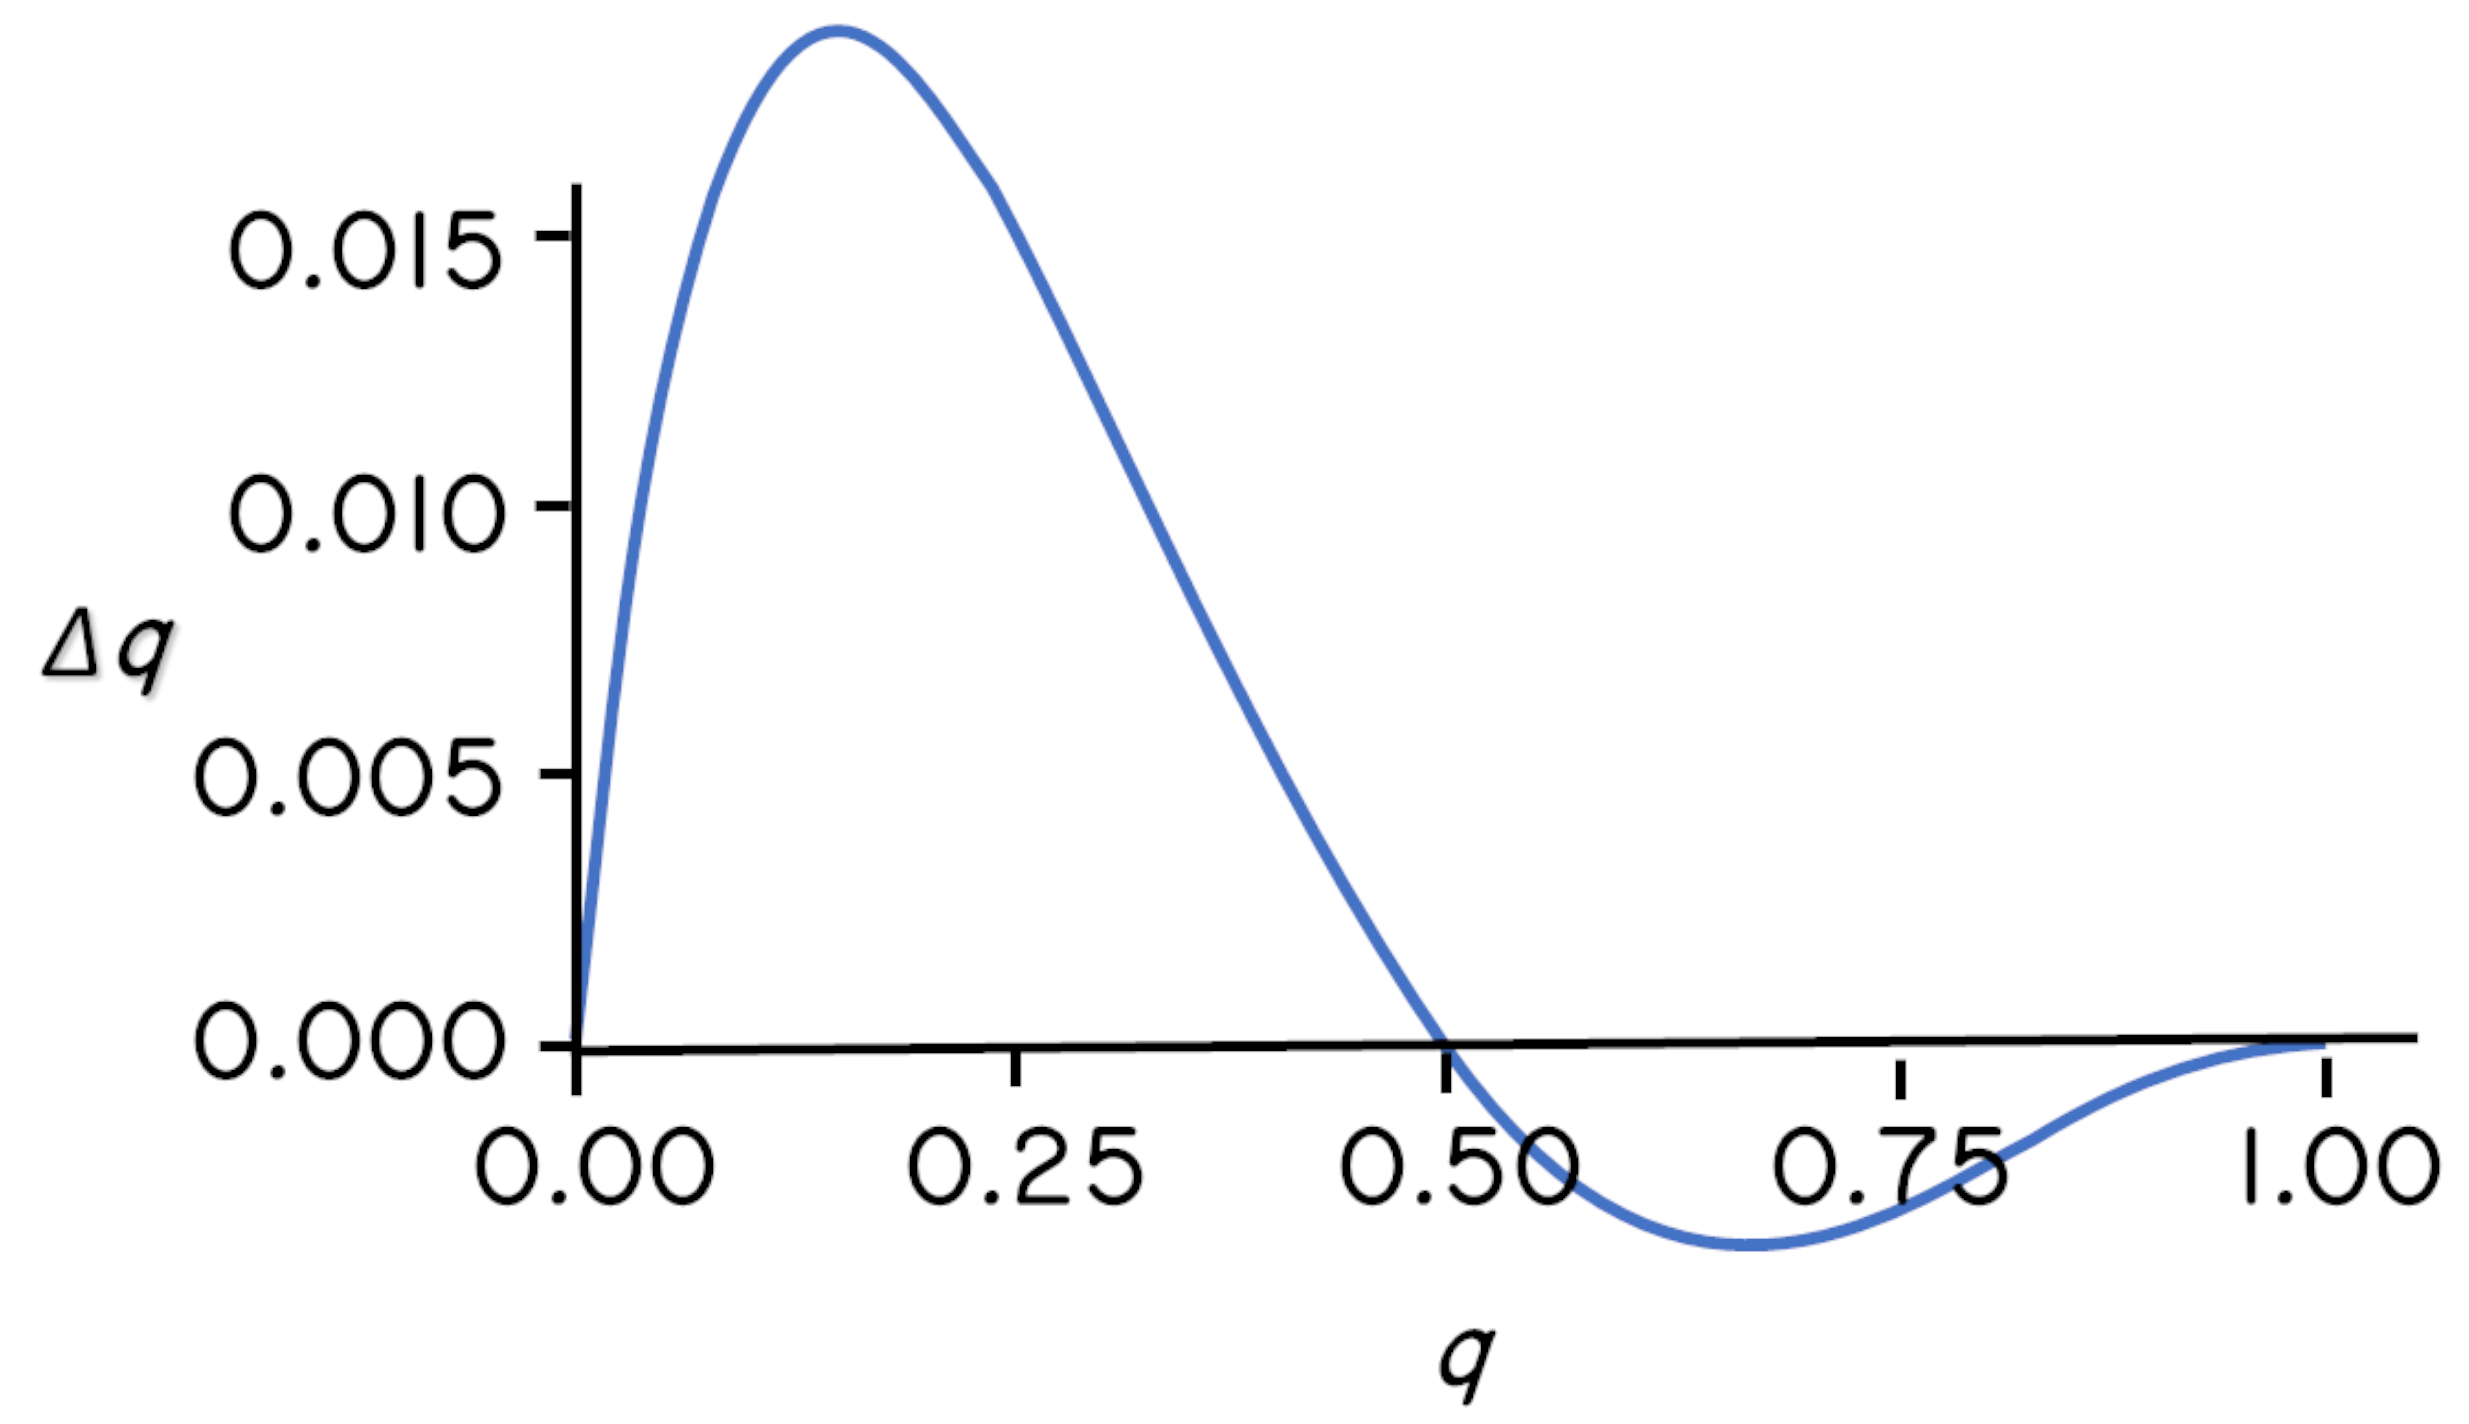
\includegraphics[width=0.65\textwidth,height=\textheight]{images/fig2-5_hr.png}

}

\caption[Prout's model of dominance]{\(\Delta q\) as a function of \(q\)
for Prout's model of dominance}

\end{figure}%

\bookmarksetup{startatroot}

\chapter{Contrasting the Ecological Hypotheses}\label{sec-eco-hyp-cont}

\begin{center}
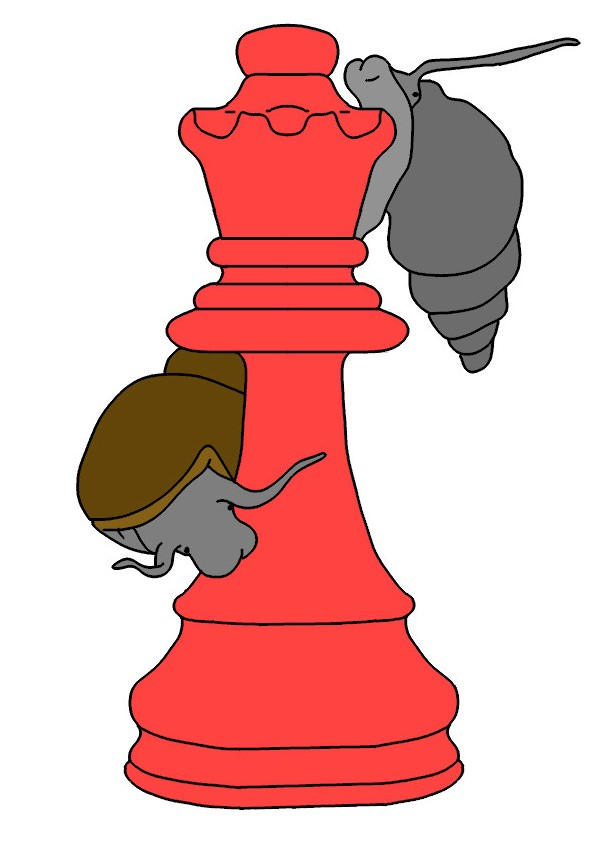
\includegraphics[width=0.33\textwidth,height=\textheight]{images/fig3-1.jpeg}
\end{center}

As I mentioned in Chapter~\ref{sec-why-sex}, my dissertation focused on
intertidal communities. I was especially interested in how two different
barnacle morphs coexisted on rocky intertidal shores in the Northern
Gulf of California. I had initially assumed that the two types were
genetically determined and that they were likely to be different species
(Figure~\ref{fig-3-2}). However, after years of false starts,\footnote{I
  ran two years of field experiments designed to test for random
  settlement by genetically determined morphs. I also ran experiments
  designed to test for habitat selection by genetically determined
  morphs. The results were always negative. I finally tested for
  predator-induced development of the bent morph by placing
  \emph{Acanthina} snails in quadrats where juvenile barnacles had
  recently settled. I used herbivorous snails as a control. The results
  showed that the presence of \emph{Acanthina} induced development of
  the bent form, but the herbivorous snails did not. It was a thrilling
  discovery.} I found that one of the two morphs was induced by chemical
cues released by a predatory snail (Figure~\ref{fig-3-3}), and that the
induced morph was more resistant to attack by this predator
(\citeproc{ref-lively1986c}{1986c}).\footnote{Plasticity is more
  mainstream now than it was in the 1980s. One reviewer of my paper was
  incredulous and recommended rejection from \emph{Evolution} because
  the bent morph was not ``genetically determined.'' The Associate
  Editor (John Endler) rejected the review and accepted the paper.
  Clearly, it is the developmental strategy that is genetically
  determined, not the morph per se (\citeproc{ref-hazel2004a}{Hazel
  \emph{et al.} 2004}; see also \citeproc{ref-lively2000a}{Lively
  \emph{et al.} 2000}).} Hence, the two morphs are not different
species, but rather the result of phenotypic plasticity. In a blink of a
field season, I went from being a community ecologist to an evolutionary
biologist.

But why two morphs? Why didn't selection favor unconditional development
of the predator-resistant morph? Using predator-exclusion cages, I found
that predation was concentrated near crevices in the reef, which the
snails used during high tide as refuges
(\citeproc{ref-lively1986b}{1986b}). As the tide receded, the snails
moved out from these crevices onto the exposed rock surfaces to forage
on barnacles. When the tide returned, the snails motored back to the
crevices, presumably to hide from snail-crushing rays that came in with
the tide. This back-and-forth movement of snails created high-predation
zones near crevices and low-predation zones far from crevices (about
20cm away). This finding explained why the predation-resistant morph was
almost always found near crevices. Field experiments also showed that
the predator-resistant morph grew more slowly and was less fecund than
the typical volcano-shaped morph (\citeproc{ref-lively1986b}{Lively
1986b}). Hence there is a trade-off. Taken together, the results
suggested that plastic development was favored by natural selection to
survive in the high-predation zones (Section~\ref{sec-app-3}). I would
later come to think of adaptive plasticity as a type of variation
strategy. Sexual reproduction can also be seen as a type of variation
strategy (\citeproc{ref-lloyd1984a}{Lloyd 1984}). And I was very
fortunate to be able to study sexual reproduction after moving to New
Zealand.

\begin{figure}

\centering{

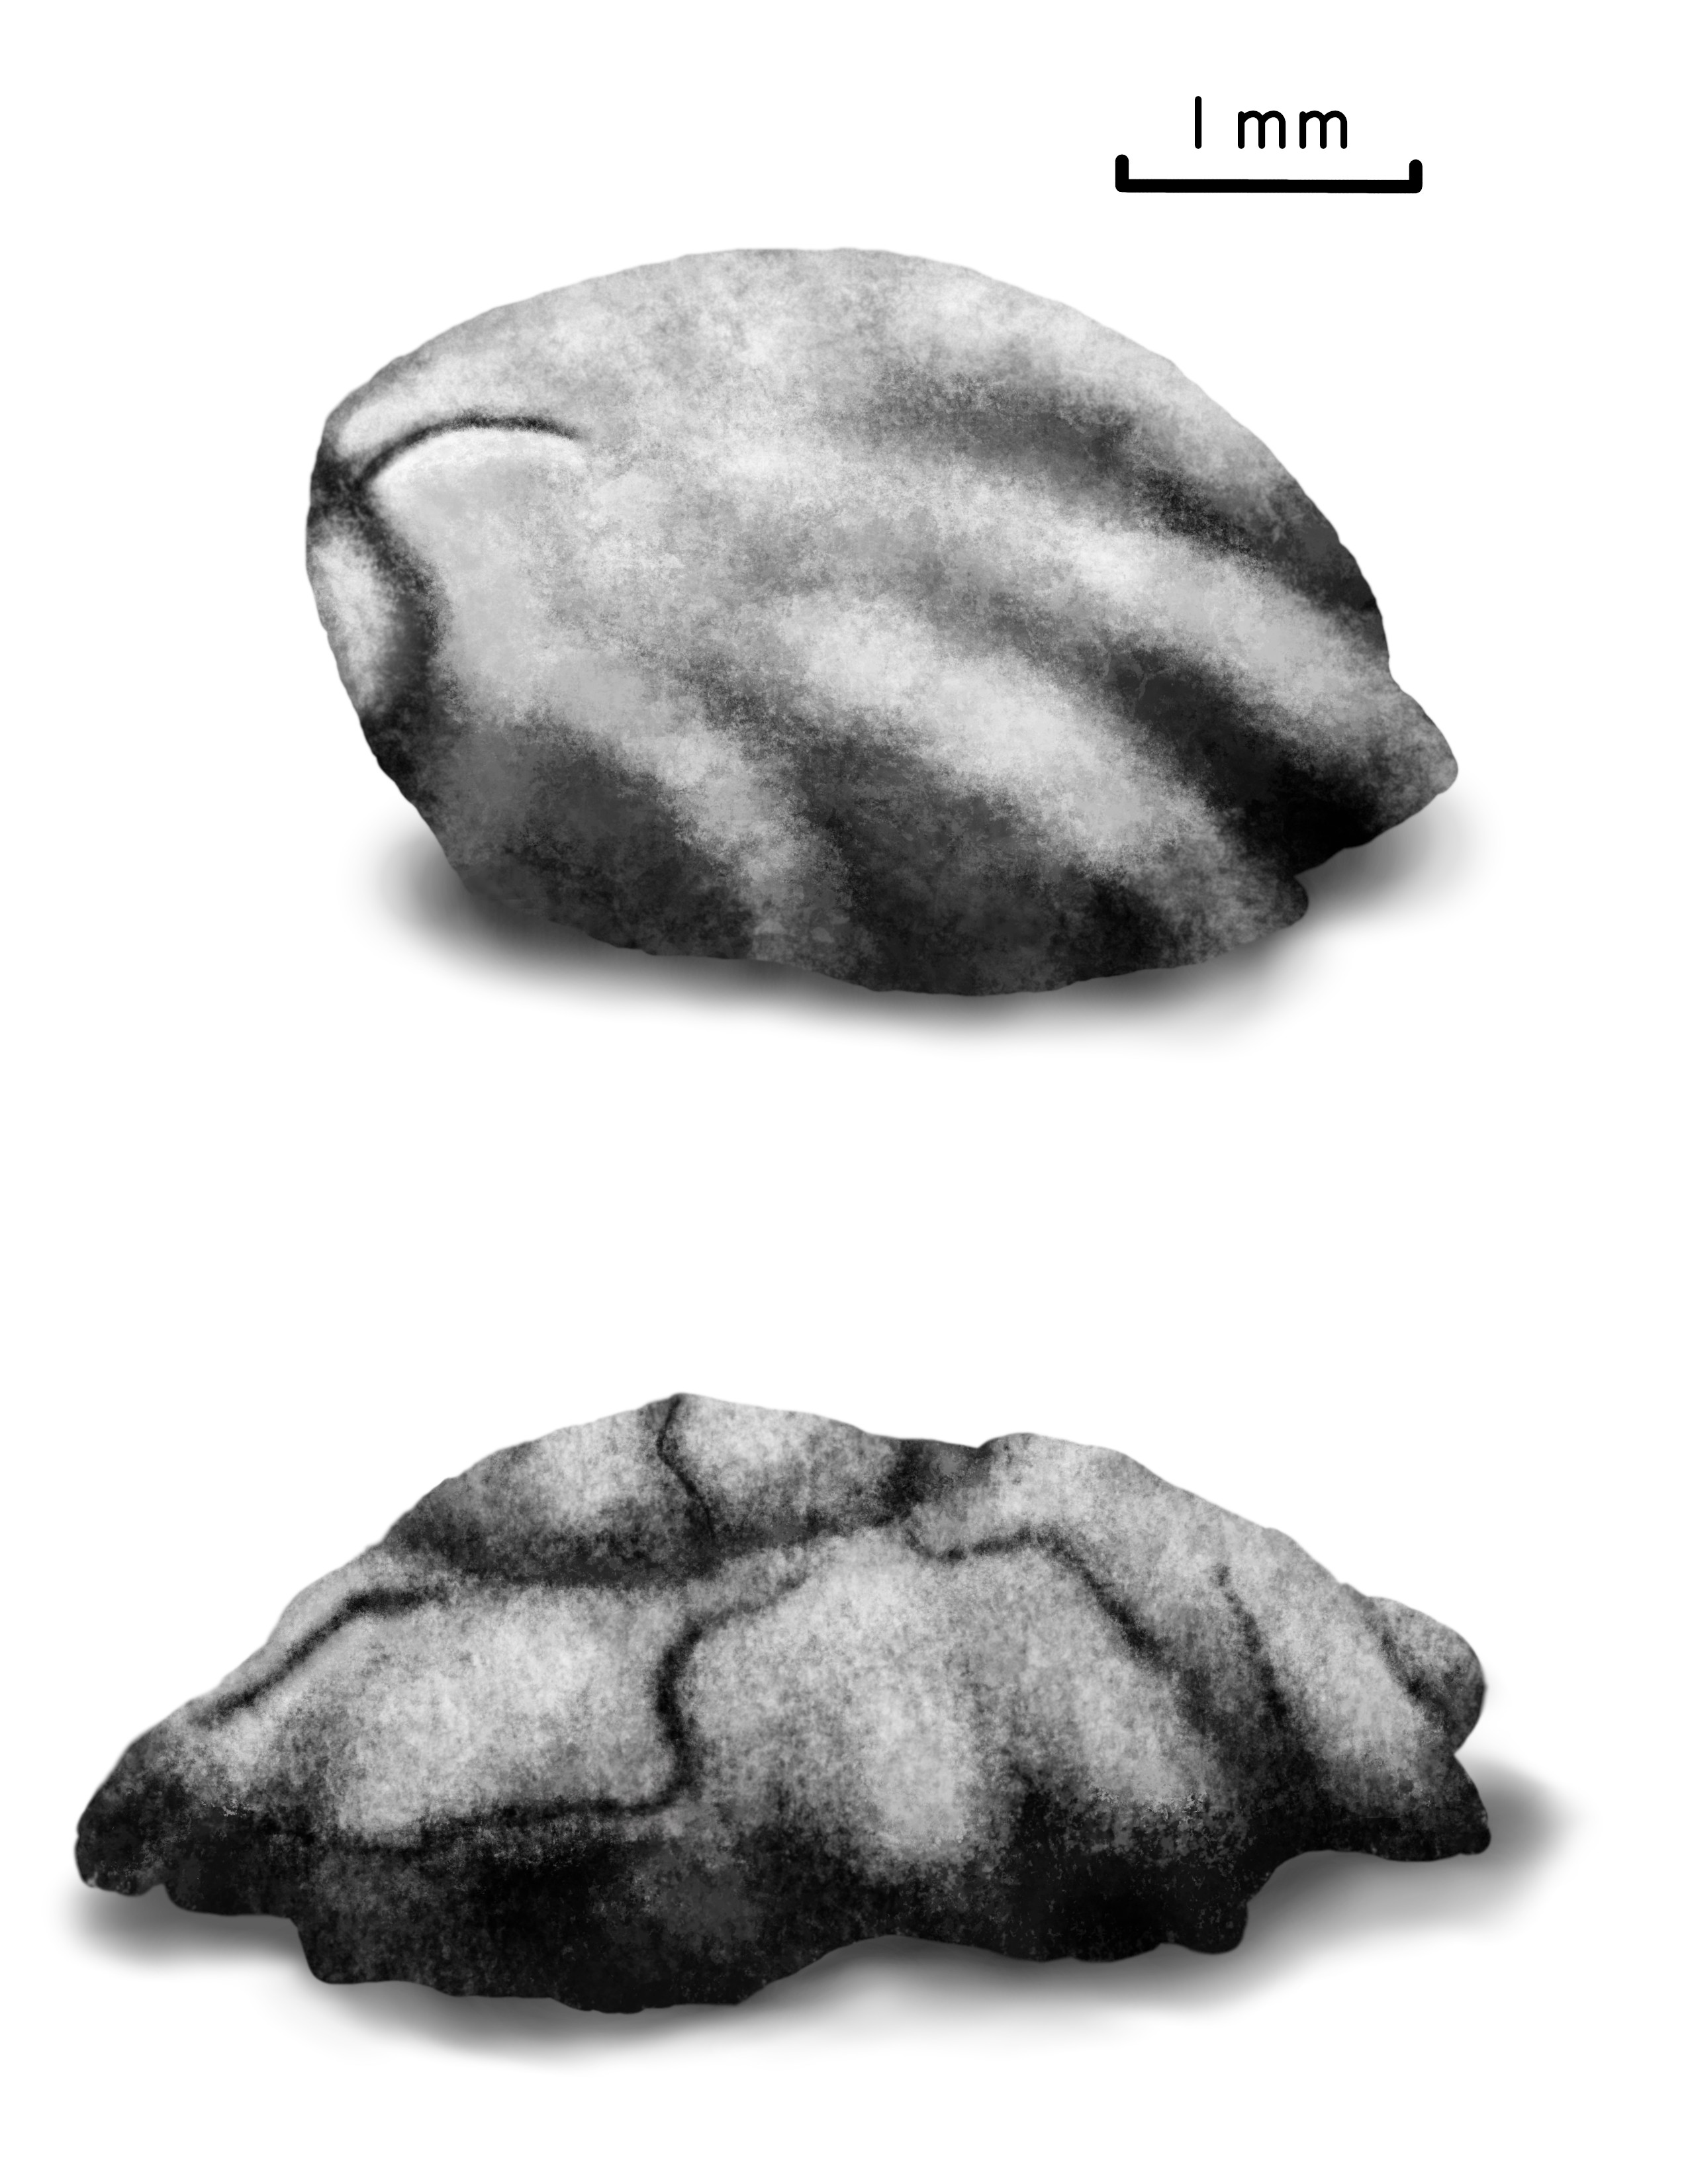
\includegraphics[width=0.3\textwidth,height=\textheight]{images/fig3-2.jpeg}

}

\caption[The two morphs of the intertidal barnacle, \emph{Chthamalus
anisopoma}]{\label{fig-3-2}The two morphs of the intertidal barnacle,
\emph{Chthamalus anisopoma}. \textbf{Top}, the ``bent'' form is induced
by exposure to chemical cues released by a specialized barnacle
predator, the predatory gastropod \emph{Acanthina angelica}. The bent or
``hooded'' form reduces the risk of successful attack by this predator.
\textbf{Bottom}, the typical, conic form of the barnacle. The conic form
is more fecund per unit size, and it grows more rapidly than the bent
form, but it is also more susceptible to attack by the predator. Drawing
by ZMD.}

\end{figure}%

\begin{figure}

\centering{

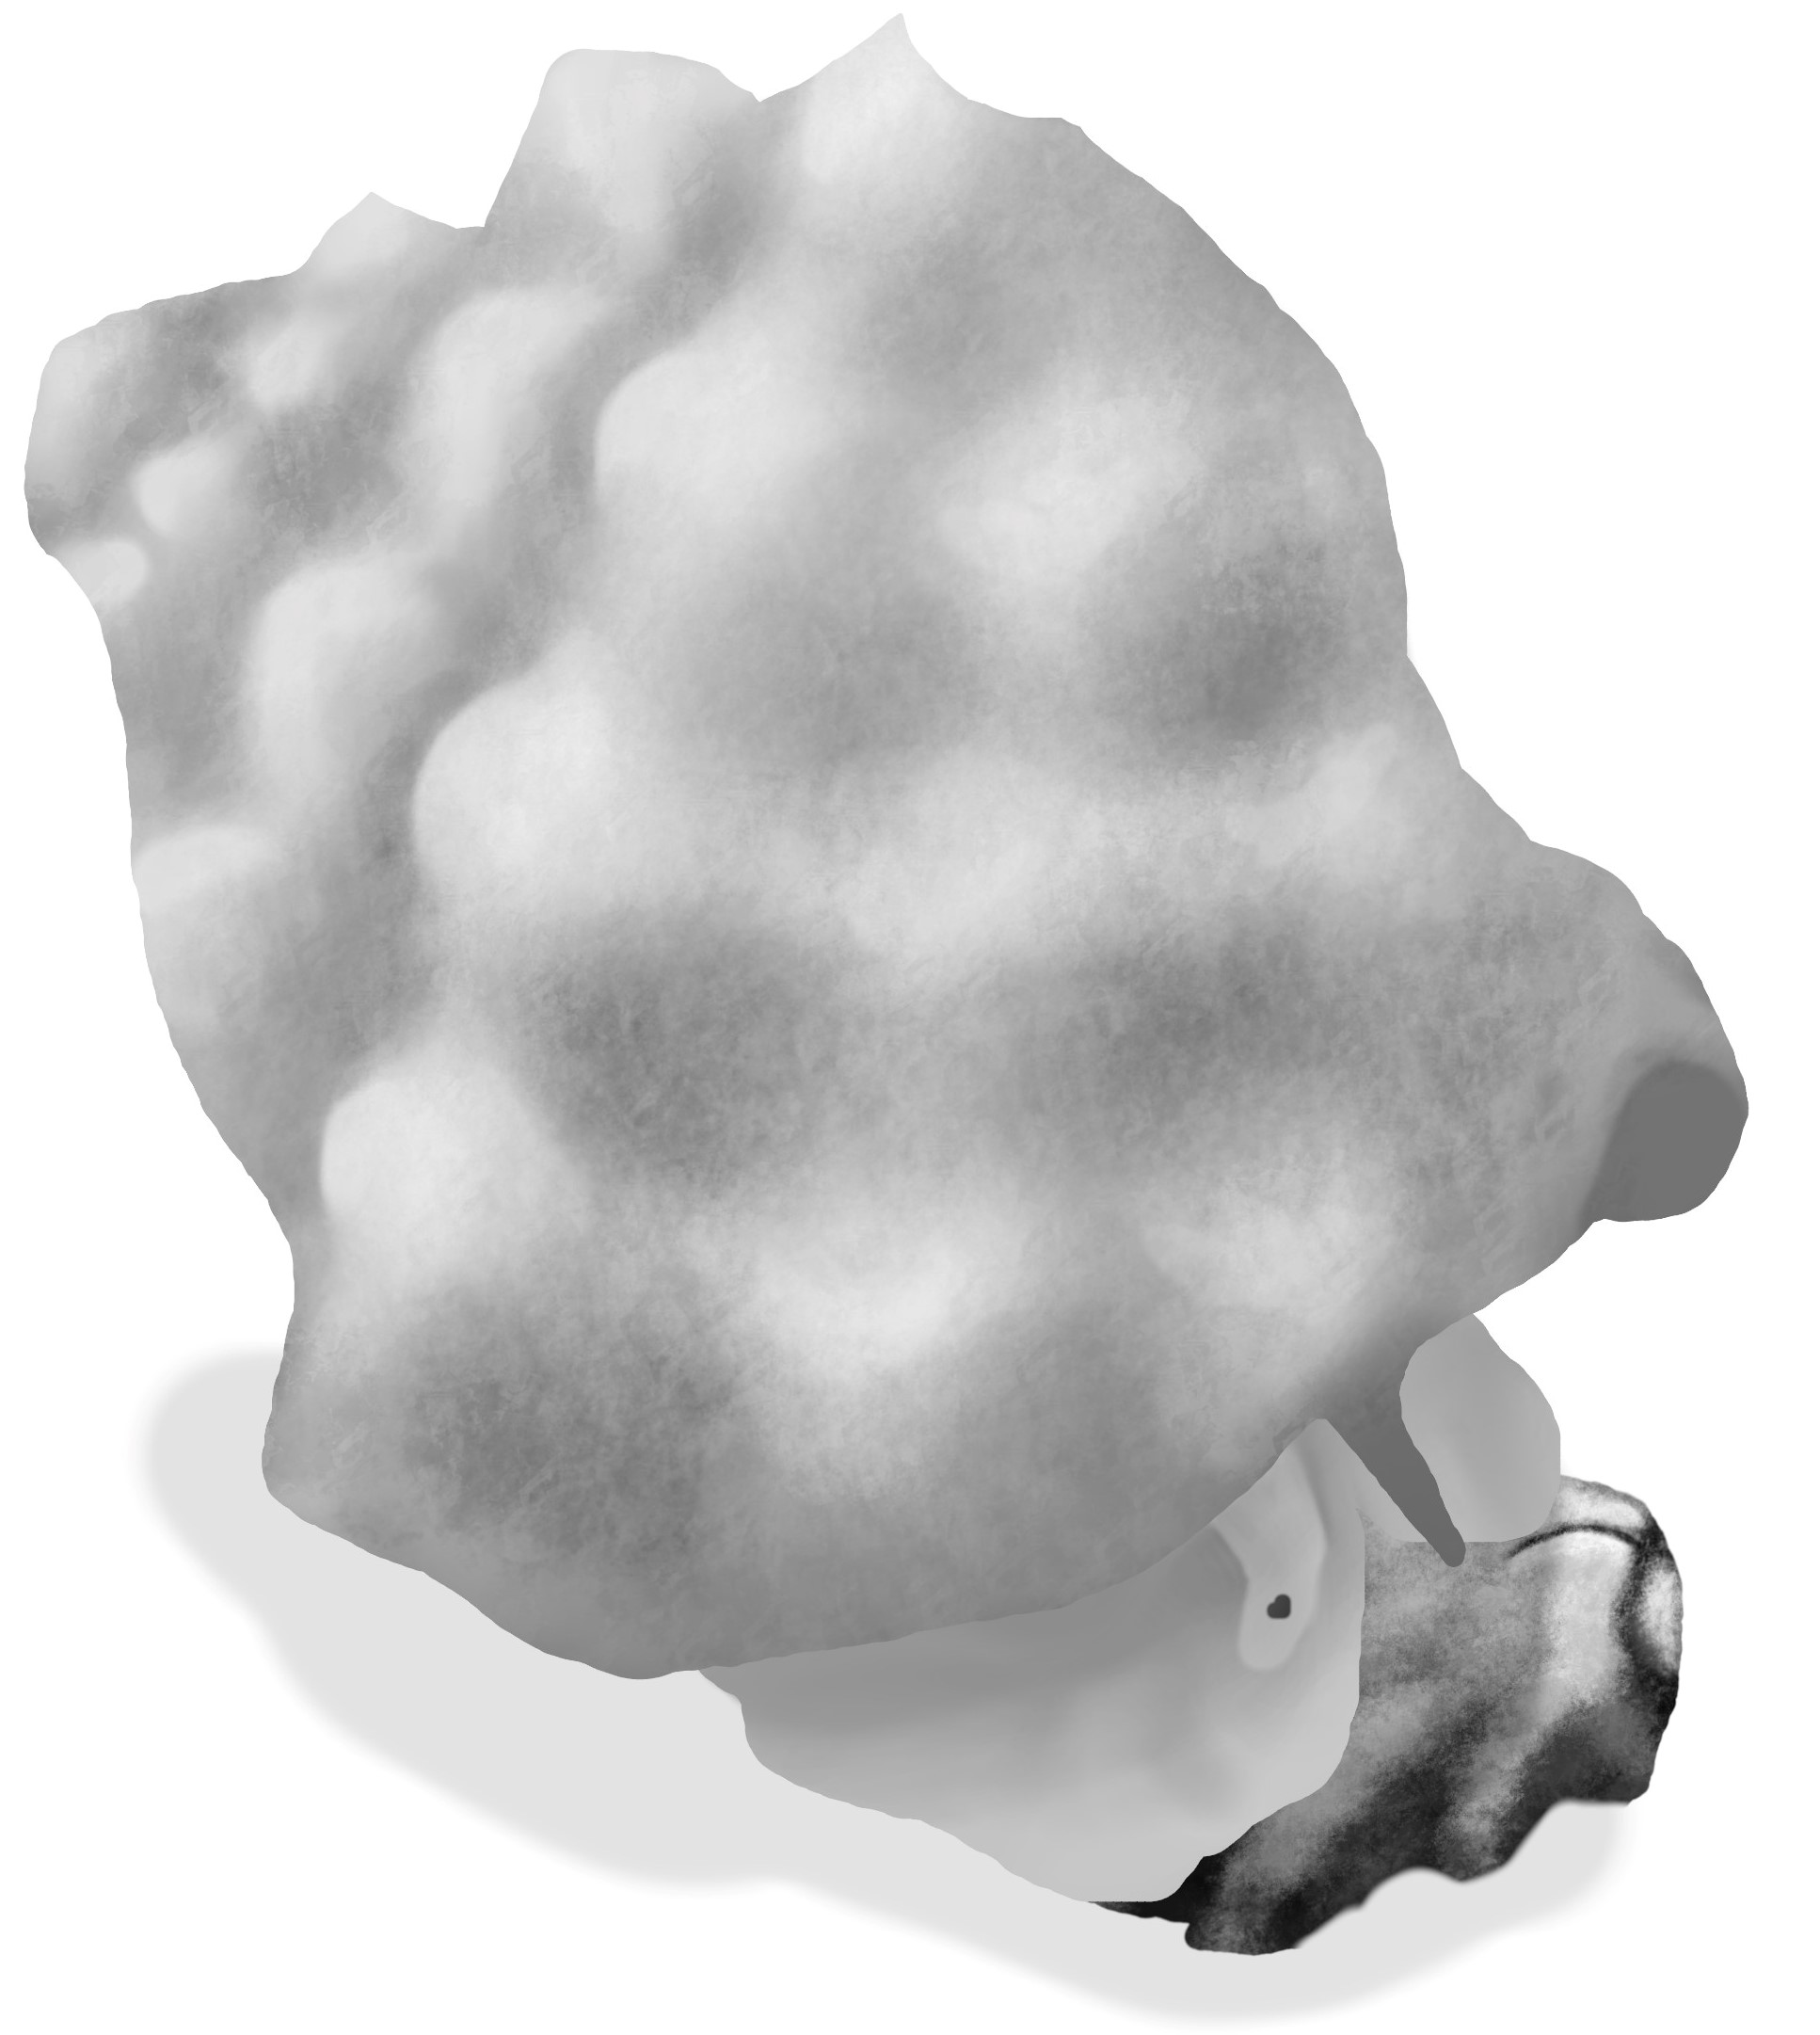
\includegraphics[width=0.3\textwidth,height=\textheight]{images/fig3-3.jpeg}

}

\caption[Drawing of the predatory snail, \emph{Acanthina angelica},
attacking the bent form of the barnacle]{\label{fig-3-3}Line drawing of
the predatory snail \emph{Acanthina angelica} attacking the bent form of
the barnacle. Note that the predator has a spine on the outer margin of
its shell. The spine is used to push through the opercular plates of
barnacles, and it is very effective at penetrating and consuming the
volcano-shaped form of the barnacle. The bent form of the barnacle is
more resistant to attack of this kind because its aperture is less open
to attack from above. Drawing by ZMD.}

\end{figure}%

I moved to New Zealand in 1984 just after defending my dissertation. My
reason for moving to New Zealand was simple: my spouse (Lynda Delph) was
there. Lynda had moved to New Zealand to study the evolution of plant
breeding systems with Professor David Lloyd. I did not have a job, but
Lynda had a small stipend from the Fulbright Foundation. By the time I
moved to New Zealand, we had only 12 dollars. But Lynda had found a flat
in a dormitory at the University of Canterbury, where she worked as a
``tutor.'' Tutors at the time were usually graduate students who served
as mentors for the resident students. We made many good friends during
our time as tutors, and it was a fascinating total immersion into Kiwi
culture. We did not have to pay rent, and we could eat for free in the
cafeteria. We could then spend Lynda's small Fulbright stipend on
sampling trips.

Then I got very lucky. I was awarded a three-year postdoctoral
fellowship from the New Zealand University Grants Committee. I had
applied to work on the evolution of facultatively parthenogenetic
nematodes, which represented a combination of my interests in
developmental plasticity and sex.\footnote{Facultative parthenogenesis
  is used to mean environmentally cued production of parthenogenetic
  females. I was originally planning to work on a nematode population
  that produced a mixture of sexual males and females at high density
  but only parthenogenetic females at low density.} These topics were
also very interesting to Wally Clark, a conceptual pioneer in the
evolution of plasticity. He was also head of the Zoology Department at
the University of Canterbury. I would not have received funding without
the support of Professor Clark. To my mind, the value of Clark's work
remains underestimated in general, but it had a big influence on me
(e.g., \citeproc{ref-clark1976a}{Clark 1976}).

I began looking for natural systems to study facultative
parthenogenesis.\footnote{We were trained ask questions first and then
  seek suitable organisms to address the questions. This was the
  tradition before model-systems research took over
  (\citeproc{ref-churchill1997a}{Churchill 1997}).} To this end, I was
reading Graham Bell's (\citeproc{ref-bell1982a}{1982}) incredible book
on the evolution and genetics of sexual reproduction. Searching the
index, I found a reference to \emph{Potamopyrgus antipodarum}, a New
Zealand freshwater snail. Bell had cited Mike Winterbourn's
(\citeproc{ref-winterbourn1970a}{1970}) dissertation work on this snail.
Luckily for me, Professor Winterbourn was just down the hall from me. I
took the book to him, and I asked if the snails were, in fact,
facultatively parthenogenetic. He said no; the snails were probably
obligate asexuals, based on lab rearing experiments that he had done. He
also said that most populations were all female, but some contained
males. He then added that there was no obvious pattern to the
distribution of males. Amazing! I immediately decided to work on these
snails.\footnote{Professor Winterbourn was supportive of my work from
  this first day. He shared his knowledge of the snail system and of
  freshwater ecology, in general, with great enthusiasm. In addition,
  Mike met with my Ph.D.~students and took them into the field. This
  book would not have been possible without Professor Winterbourn.}

\section{The Method of Multiple Working
Hypotheses}\label{the-method-of-multiple-working-hypotheses}

As graduate students at the University of Arizona, we read some of the
classics in the history and philosophy of science. Two of these papers
concerned the method of contrasting multiple working hypotheses
(\citeproc{ref-chamberlin1890a}{Chamberlin 1890};
\citeproc{ref-platt1964a}{Platt 1964}).\footnote{See also Elliott and
  Brook (\citeproc{ref-elliott2007a}{2007}). They point out crucial
  differences between Chamberlin and Platt including that Chamberlin
  allowed for multiple ideas to be partially correct, which is important
  for Chapter~\ref{sec-chap6}.} The idea is that multiple hypotheses
should be simultaneously considered. Then, to the extent possible, the
alternatives are forced to make different \emph{a priori} predictions
about the possible results. The hope is that all but one of the
alternative hypotheses would be eliminated, leading to a ``strong
inference'' that the remaining hypothesis is supported
(\citeproc{ref-platt1964a}{Platt 1964}). Thus, the focus is on
falsifying one or more of the alternatives, rather than proving one of
them (\citeproc{ref-popper1959a}{Popper 1959}). Graham Bell used this
same method to contrast the ecological models for sex by using data on
the geographic distribution of asexual individuals across many plant and
animal taxa (\citeproc{ref-bell1982a}{Bell 1982}). The data led him to
reject the Lottery Model (Chapter~\ref{sec-eco-hyp}). I decided to focus
a similar test directly on the New Zealand snails
(Figure~\ref{fig-3-4}).

\begin{figure}

\centering{

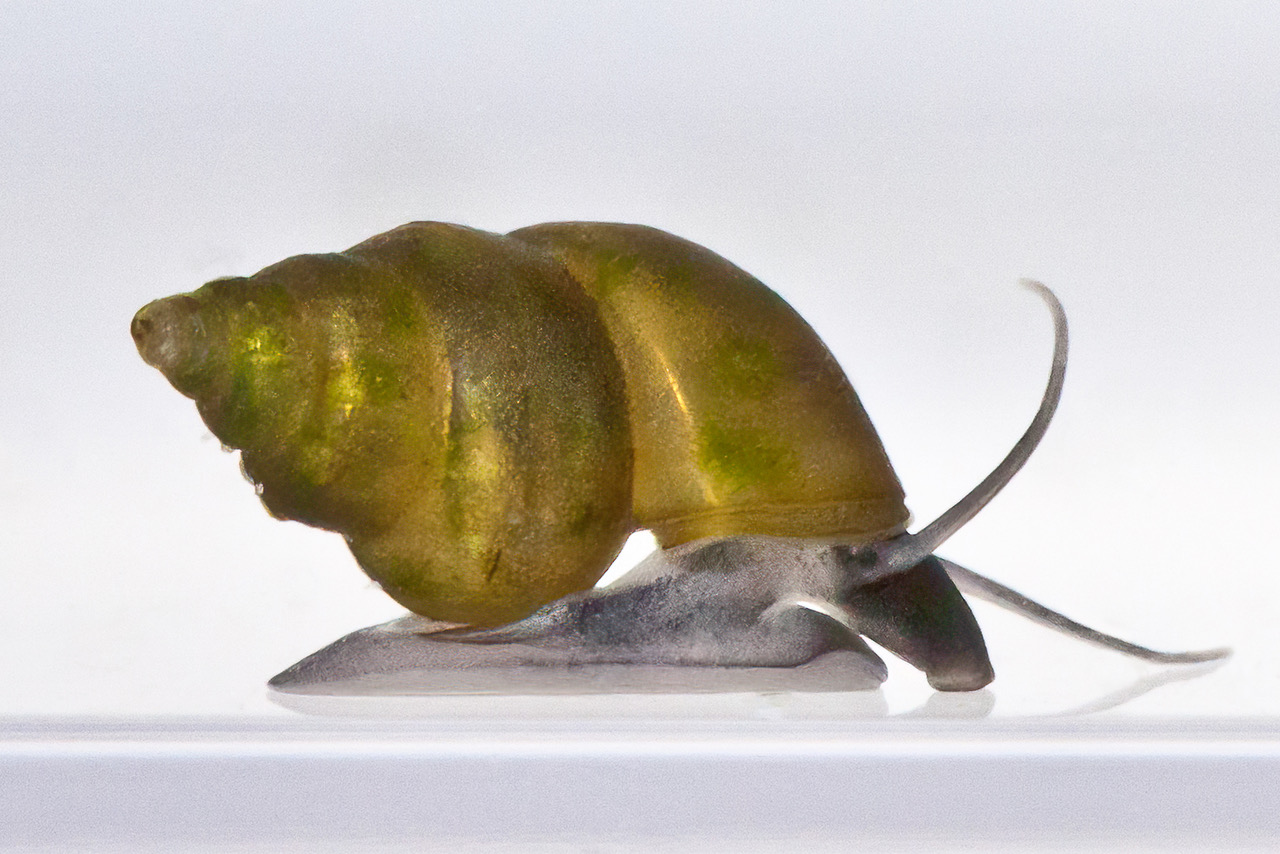
\includegraphics[width=0.6\textwidth,height=\textheight]{images/fig3-4.jpeg}

}

\caption[The freshwater snail \emph{Potamopyrgus
antipodarum}]{\label{fig-3-4}\textbf{Photo credit: ©
\href{https://www.bartzijlstra.com}{Bart Zijlstra}. Used by permission.}
The freshwater snail \emph{Potamopyrgus antipodarum}. This small (3--6
mm) prosobranch snail evolved from marine ancestors
(\citeproc{ref-phillips1990a}{Phillips \& Lambert 1990}). Associated
with the invasion of freshwater, the snail evolved an internal brood
pouch, where the embryos hatch and develop before crawling out as
juveniles. The snail also evolved parthenogenetic reproduction.
Parthenogenesis and brooding are both rare traits in invertebrates, but
they are often found together (\citeproc{ref-lively1994b}{Lively \&
Johnson 1994}). Some \emph{P. antipodarum} populations presently consist
of a mixture of diploid sexual individuals and polyploid asexual
females. The question under consideration here is, why have the sexual
females persisted in these mixed population snails? What are the
advantages of sexual reproduction?}

\end{figure}%

The snails (\emph{Potamopyrgus antipodarum}) are often called mud
snails, but I think the term is a misnomer. They live on rocks and
vegetation in some of the most beautiful clear lakes, rivers, and
streams in New Zealand (``Potamo'' means river, not mud, in Greek). In
any case, based on Winterbourn's ecological work, streams seemed more
unstable than lakes, as water flow can vary dramatically, especially
during heavy rains in the mountains
(\citeproc{ref-winterbourn1981a}{Winterbourn \emph{et al.} 1981}).
Hence, under the Lottery Model, streams should have more sexual females
(and males) than lakes, because streams have more disturbance and less
competition (see Chapter~\ref{sec-eco-hyp} for a comparison of models).
By contrast, it seemed that competition for resources should be greater
in lakes than in streams. Indeed, lake populations of the snail can be
extremely dense. So, under the Tangled Bank, there should be more sexual
females in lakes, where competition for resources is expected to be
high. Finally, under the Red Queen Hypothesis, there should be more
sexual females where the risk of infection by coevolving parasites is
higher. As such, the different hypotheses could be forced to make
different predictions, with the important caveat that infection might be
correlated with habitat.

Some clarification regarding the prediction of the Red Queen Hypothesis
might be useful here. Some people have asked me why the correlation
between sex and infection is expected to be positive if, indeed,
parasites are the selective force for sexual reproduction. For example,
one could ask, if sex is so helpful in reducing infection risk, then
shouldn't the highly sexual populations have fewer, not more, parasites?
That could, of course, be expected in an experiment where hosts across
all populations were exposed to the same number of parasites. Then the
more genetically diverse populations with higher frequencies of sexual
females might be expected to have a lower prevalence of infection. But
it is not the case that all natural populations have the same risk of
infection. The idea under the Red Queen Hypothesis is that asexual
females would replace sexual females where the risk of infection is low,
and that sexual females would persist where the risk of infection is
high, provided that the parasites are highly virulent. That is how the
positive correlation could be generated. Nonetheless, the data could be
expected to be very messy, especially if the frequency of sex oscillates
over time in response to coevolutionary games with parasites.

The snails are infected by trematode worms, but I did not know anything
about trematodes when I first began dissecting snails. I was just
looking for males. Winterbourn told me that I would know a male snail
when I saw one, as they have a penis just behind the right tentacle. But
I had not observed any such structure on the many snails I collected
from the streams around the university. I was beginning to think that I
was missing something. Then one day, when I was dissecting a snail,
hundreds of swimming things came out. Sperm, I thought. My first male! I
took them to Wally Clark's research technician, Jan McKenzie, to put
under her fancy microscope. She informed me that sperm do not have eyes,
that they do not have spines on their tails, and that they are, in fact,
orders of magnitude smaller than these wiggling beasts under her lens.
She was not impressed. I had perfectly fit the Kiwi stereotype of North
American ecologists: good with statistics but no knowledge of real
animals. She informed me that these swimming things were trematode
larvae, \textbf{sterilizing parasites} of snails. Happily, we remained
good friends, despite her disappointment in my training. And I had found
my first infection, which meant that I might be able to test the Red
Queen.

Perhaps embarrassingly, I had a scientific bias against the Red Queen
going into the study. My bias was based on a study by May and Anderson
(\citeproc{ref-may1983a}{May \& Anderson 1983}). They showed that
parasites had to kill infected individuals for sex to be favored over
asex in hosts. Parasites are usually not that virulent; hence, it seemed
to me that parasites could not provide sufficiently strong selection to
\emph{generally} favor sex. I will return to this important paper in
another chapter and discuss how key assumptions of their model have been
relaxed.

\subsection{A side story on JMS}\label{a-side-story-on-jms}

John Maynard Smith (JMS) was one of the most influential theoretical
biologists in history of evolutionary thought. He was able to formulate
and communicate novel ideas with apparent ease. Around the time that I
was beginning to work on \emph{Potamopyrgus}, JMS came to New Zealand,
along with his wife, Sheila. He was invited by David Lloyd to spend time
at University of Canterbury and to deliver three public lectures, which
were all fantastic. During this time, JMS spent several weeks in New
Zealand. Lynda, David, and I were lucky enough to hang out with him
quite a bit. JMS was a remarkable individual. He could talk with anyone
and show a sincere interest in their work. One morning, I was sitting
next to JMS in the tearoom in the old Zoology Department. I was scared
speechless. He kindly asked me what I was working on, so I told him
about the snails. He knew of them! In fact, he had covered them in his
book, \emph{The Evolution of Sex}.\footnote{With respect to
  \emph{Potamopyrgus} (along with a parthenogenetic beetle) Maynard
  Smith (\citeproc{ref-maynard1978a}{1978}) wrote, ``Further
  Investigations of these cases could be most interesting.'' When I met
  JMS, I did not know (or did not remember) that he had written this.
  But I think that he was correct.} He was very excited that I was
working on these creatures, and he wanted to know my plan. I told him of
my rough ideas for looking at the distribution of males as a way of
contrasting the ecological hypotheses for sex. He looked directly at me,
and said, ``Interesting, but I hope the answer is not parasites'' (or
something like that). I asked him, why not parasites? He laughed out
loud, and with a big smile he said: ``Because Bill Hamilton thought of
it first!'' I could tell he was kidding. He then encouraged me to take
the project on, and then he laughed again and added, ``Whatever you do,
don't go and solve the problem of sex. Sex is too much bloody fun to
have an answer!''

Toward the end of their time in New Zealand, JMS, Sheila, David, Lynda,
and I did a trip together around the South Island. The whole time was
incredible. Just listening to David and John talk about evolutionary
theory was a scientific dream. Towards the end of our trip, we were all
together in a restaurant at the Hermitage (near Mt. Cook) on the night
that JMS turned 65 and formally retired. Our server, a young alpinist
working to support his climbing in the Southern Alps, asked JMS, ``I
think that I saw a documentary about you. Are you famous?'' JMS (smiling
and intrigued) asked the alpinist what he remembered. Without
hesitation, the alpinist recited a perfect overview of evolution by
natural selection. JMS was clearly touched. Almost exactly half-way
around the world from Sussex England, in a small township in New
Zealand, JMS met someone whom he had influenced with his work. And this
was on the very night of his retirement.

The next day, we drove to a small lake near Mt. Cook that David knew
about: Lake Alexandrina. It was a glorious day, and we decided that we
might as well collect some snails. JMS waded into the water and
proceeded to collect a handful of \emph{Potamopyrgus} from the shallow
rocks. He handed the snails to me. He then laughed and said, ``When you
publish your study, I want to know the outcome for these exact snails.''
As it turned out, Lake Alexandrina has a mixed population of sexual and
asexual snails, and it has been the primary focus of our long-term
studies on \emph{Potamopyrgus}. The snail team still refers to this
original site of collection as ``JMS.'' Interestingly, JMS is one of the
most dynamic sites in the whole lake.

\section{The Distribution of Male
Snails}\label{the-distribution-of-male-snails}

To contrast the alternative ecological hypotheses, I sampled snails from
lakes and streams across the South Island of New Zealand. I could drive
Lynda's Volkswagen bug to most of the lakes, but I had to backpack into
many. Unfortunately, my time working in the Sonoran Desert had not
prepared me for the steep climbs, heavy rains, and chest-deep river
crossings on the South Island. I did not take enough food or dry clothes
on one trip, and my desert hiking boots disintegrated. I got my butt
kicked. But it was wonderful to have an excuse to see remote parts of
the South Island, especially after I got better gear and gained a better
understanding of the New Zealand bush.

I collected and dissected hundreds of snails from each of 29 streams and
22 lakes, mostly on the South Island. I recorded sex (male or female)
and infection by the trematodes that Winterbourn
(\citeproc{ref-winterbourn1973a}{1973}) described. I reasoned that the
frequency of males in a population must be strongly correlated with the
frequency of sexual females simply because males are only produced by
sexual females.\footnote{This assumption turned out to be not strictly
  true. Polyploid females occasionally produce males, although they seem
  unlikely to be very fertile (\citeproc{ref-soper2013a}{Soper \emph{et
  al.} 2013}).} The results showed that there were more males in lakes
than in streams, which was inconsistent with the Lottery Model, but it
was consistent with the Tangled Bank Model. However, male frequency was
better predicted by the frequency of trematode infection than by habitat
\emph{per se} (\citeproc{ref-lively1987a}{Lively 1987}). Hence,
surprisingly, the results favored the Red Queen Hypothesis. I presented
these findings to a small group at David Lloyd's flat, and they
convinced me to submit to \emph{Nature}.\footnote{The group included
  Mark McKone. Mark was a post-doc with David, and his comments were
  especially influential. Fifteen years later, I would become
  Ph.D.~advisor to one of Mark's star mentees at Carleton College,
  Maurine Neiman.}

A fascinating paper on the same topic was published in \emph{Nature} at
about the same time. This paper was also based on a strong-inference
test comparing the Red Queen and the Tangled Bank. The authors, Austin
Burt and Graham Bell (\citeproc{ref-burt1987a}{1987}), examined
recombination in mammals. They reasoned that under the Red Queen
Hypothesis, longer-lived mammals would have higher rates of
recombination because more genetic mixing would be favored as the
asymmetry in host/parasite generation time increased. In contrast, the
Tangled Bank Model predicted that shorter-lived mammals would have
higher rates of recombination because they have larger litters, and
recombination might lead to reduced competition among the more diverse
offspring. Their results were stunning. Recombination was tightly and
positively related to longevity in natural populations.\footnote{There
  we also some very interesting outliers. Domesticated mammals had very
  strong positive residuals for the rate of recombination. This result
  suggests that recombination was selected by frequent changes in the
  targets of artificial selection by humans.} The Red Queen was again
supported.

Based on these studies in \emph{Nature}, I was beginning to think that
parasites might be a factor in selecting for cross-fertilization in
hosts. But my study as well as the study of Burt and Bell
(\citeproc{ref-burt1987a}{1987}) were based on correlations. And every
scientist knows that correlation is not causation. On the other hand,
these correlations were predicted \emph{a priori} by Lloyd
(\citeproc{ref-lloyd1980a}{1980}) and others
(\citeproc{ref-bell1982a}{Bell 1982};
\citeproc{ref-glesener1978a}{Glesener \& Tilman 1978}). The Red Queen
was supported by the data, but the data were not used to generate the
hypothesis. Using the same data to both generate and substantiate
hypotheses is where the problem arises with correlation, especially when
multiple factors are considered in ``fishing expeditions.'' But forcing
different hypotheses to make different \emph{a priori} predictions about
the direction of correlations is, to my mind, a powerful way to evaluate
alternatives.

As a brief aside, I cannot help but mention the human toll taken by R.A.
Fisher's use of ``correlation is not causation'' as a way to plant doubt
in the mind of smokers about the now-obvious risks of smoking
(\citeproc{ref-gould1991a}{Gould 1991};
\citeproc{ref-stolley1991a}{Stolley 1991}). Fisher was a consultant for
the tobacco industry, and he did the industry a great service at the
cost of human lives. I would also add that no test statistic is
causation; F statistics derived from analysis of variance are not
causation. Causation might be inferred from well-designed experiments,
but no statistical test is causation. Analytical theory is not causation
either, as is well demonstrated by the theoretical literature on
sex/recombination. Causation instead may be inferred when multiple
independent lines of evidence point to similar solutions. I think that
Levins (\citeproc{ref-levins1966a}{1966}) was correct when he wrote,
``Hence our truth is the intersection of independent lies.''\footnote{From
  Levins (\citeproc{ref-levins1966a}{1966}): ``Therefore, we attempt to
  treat the same problem with several alternative models each with
  different simplifications but with a common biological assumption.
  Then, if these models, despite their different assumptions, lead to
  similar results we have what we can call a robust theorem which is
  relatively free of the details of the model. Hence our truth is the
  intersection of independent lies.''} Although he was referring
specifically to mathematical models, the same principle applies to
biological systems. Ideally, the multiple lines of evidence would
include long-term field observations of individual populations, broader
biogeographic patterns across populations, and direct experiments on
multiple independent systems, as well as multiple theoretical forays
into the conditions under which the hypothesis is expected to hold.

In any case, my view by 1987 was that the Red Queen Hypothesis merited
serious consideration.\footnote{I was also persuaded by elegant
  experimental studies on sweet vernal grass, which showed a
  density-independent advantage to having a rare genotype
  (\citeproc{ref-antonovics1984a}{Antonovics \& Ellstrand 1984};
  \citeproc{ref-ellstrand1985a}{Ellstrand \& Antonovics 1985}). Later
  studies showed that the rare advantage was likely due to escape from
  infection (\citeproc{ref-kelley1988a}{Kelley \emph{et al.} 1988};
  \citeproc{ref-kelley1993a}{1993}, \citeproc{ref-kelley1994a}{1994}).}
For my own data, I now asked whether the correlation between sex and
infection was a ``red herring.'' In other words, could the correlation
be generated because of something else? Yes, it could. Here is how it
might work. First, infection could be higher in dense host populations
as expected under theory (\citeproc{ref-anderson1979a}{Anderson \& May
1979}; \citeproc{ref-may1979a}{May \& Anderson 1979}). Second, there
might be more sex in dense populations because asexual reproduction is
favored in sparse populations as a way for individuals to ensure
reproduction even in the absence of conspecific mates
(\citeproc{ref-gerritsen1980a}{Gerritsen 1980};
\citeproc{ref-lloyd1980a}{Lloyd 1980};
\citeproc{ref-tomlinson1966a}{Tomlinson 1966}). This latter idea is
called the ``Reproductive Assurance Hypothesis.'' Hence, one could find
a positive correlation between sex and infection as a simple consequence
of epidemiology and selection for reproductive assurance. So, I decided
to sample again, this time focusing on South Island lakes
(Figure~\ref{fig-3-5} \& Figure~\ref{fig-3-6}) while also collecting
data on snail density. The results were consistent with the
epidemiological expectations, as there was a marginally significant
positive relationship between snail density and infection prevalence,
but there was no support for the Reproductive Assurance Hypothesis
(\citeproc{ref-lively1992a}{Lively 1992}). Finally, the previously
observed positive relationship between sex and infection held
(Figure~\ref{fig-3-5}).\footnote{The partial correlation between percent
  male and prevalence of infection, while controlling for habitat, is
  highly significant (\(r = 0.36\), \(P < 0.001\)). However, the partial
  correlation between percent male and habitat, while controlling for
  prevalence of infection, is marginally significant (\(r = 0.21\),
  \(P = 0.05\)). Similar results were gained after males were excluded
  from the calculation of infection prevalence, which controls for any
  sex-specific differences in susceptibility (as shown in
  Figure~\ref{fig-3-5}); specifically, prevalence of infection in
  females was significantly correlated with male frequency while
  controlling for habitat (\(r = 0.37\), \(P < 0.001\)), but the
  converse was not true (\(r = 0.19\), \(P = 0.06\)).} The Red Queen was
still in the running.

\begin{figure}

\centering{

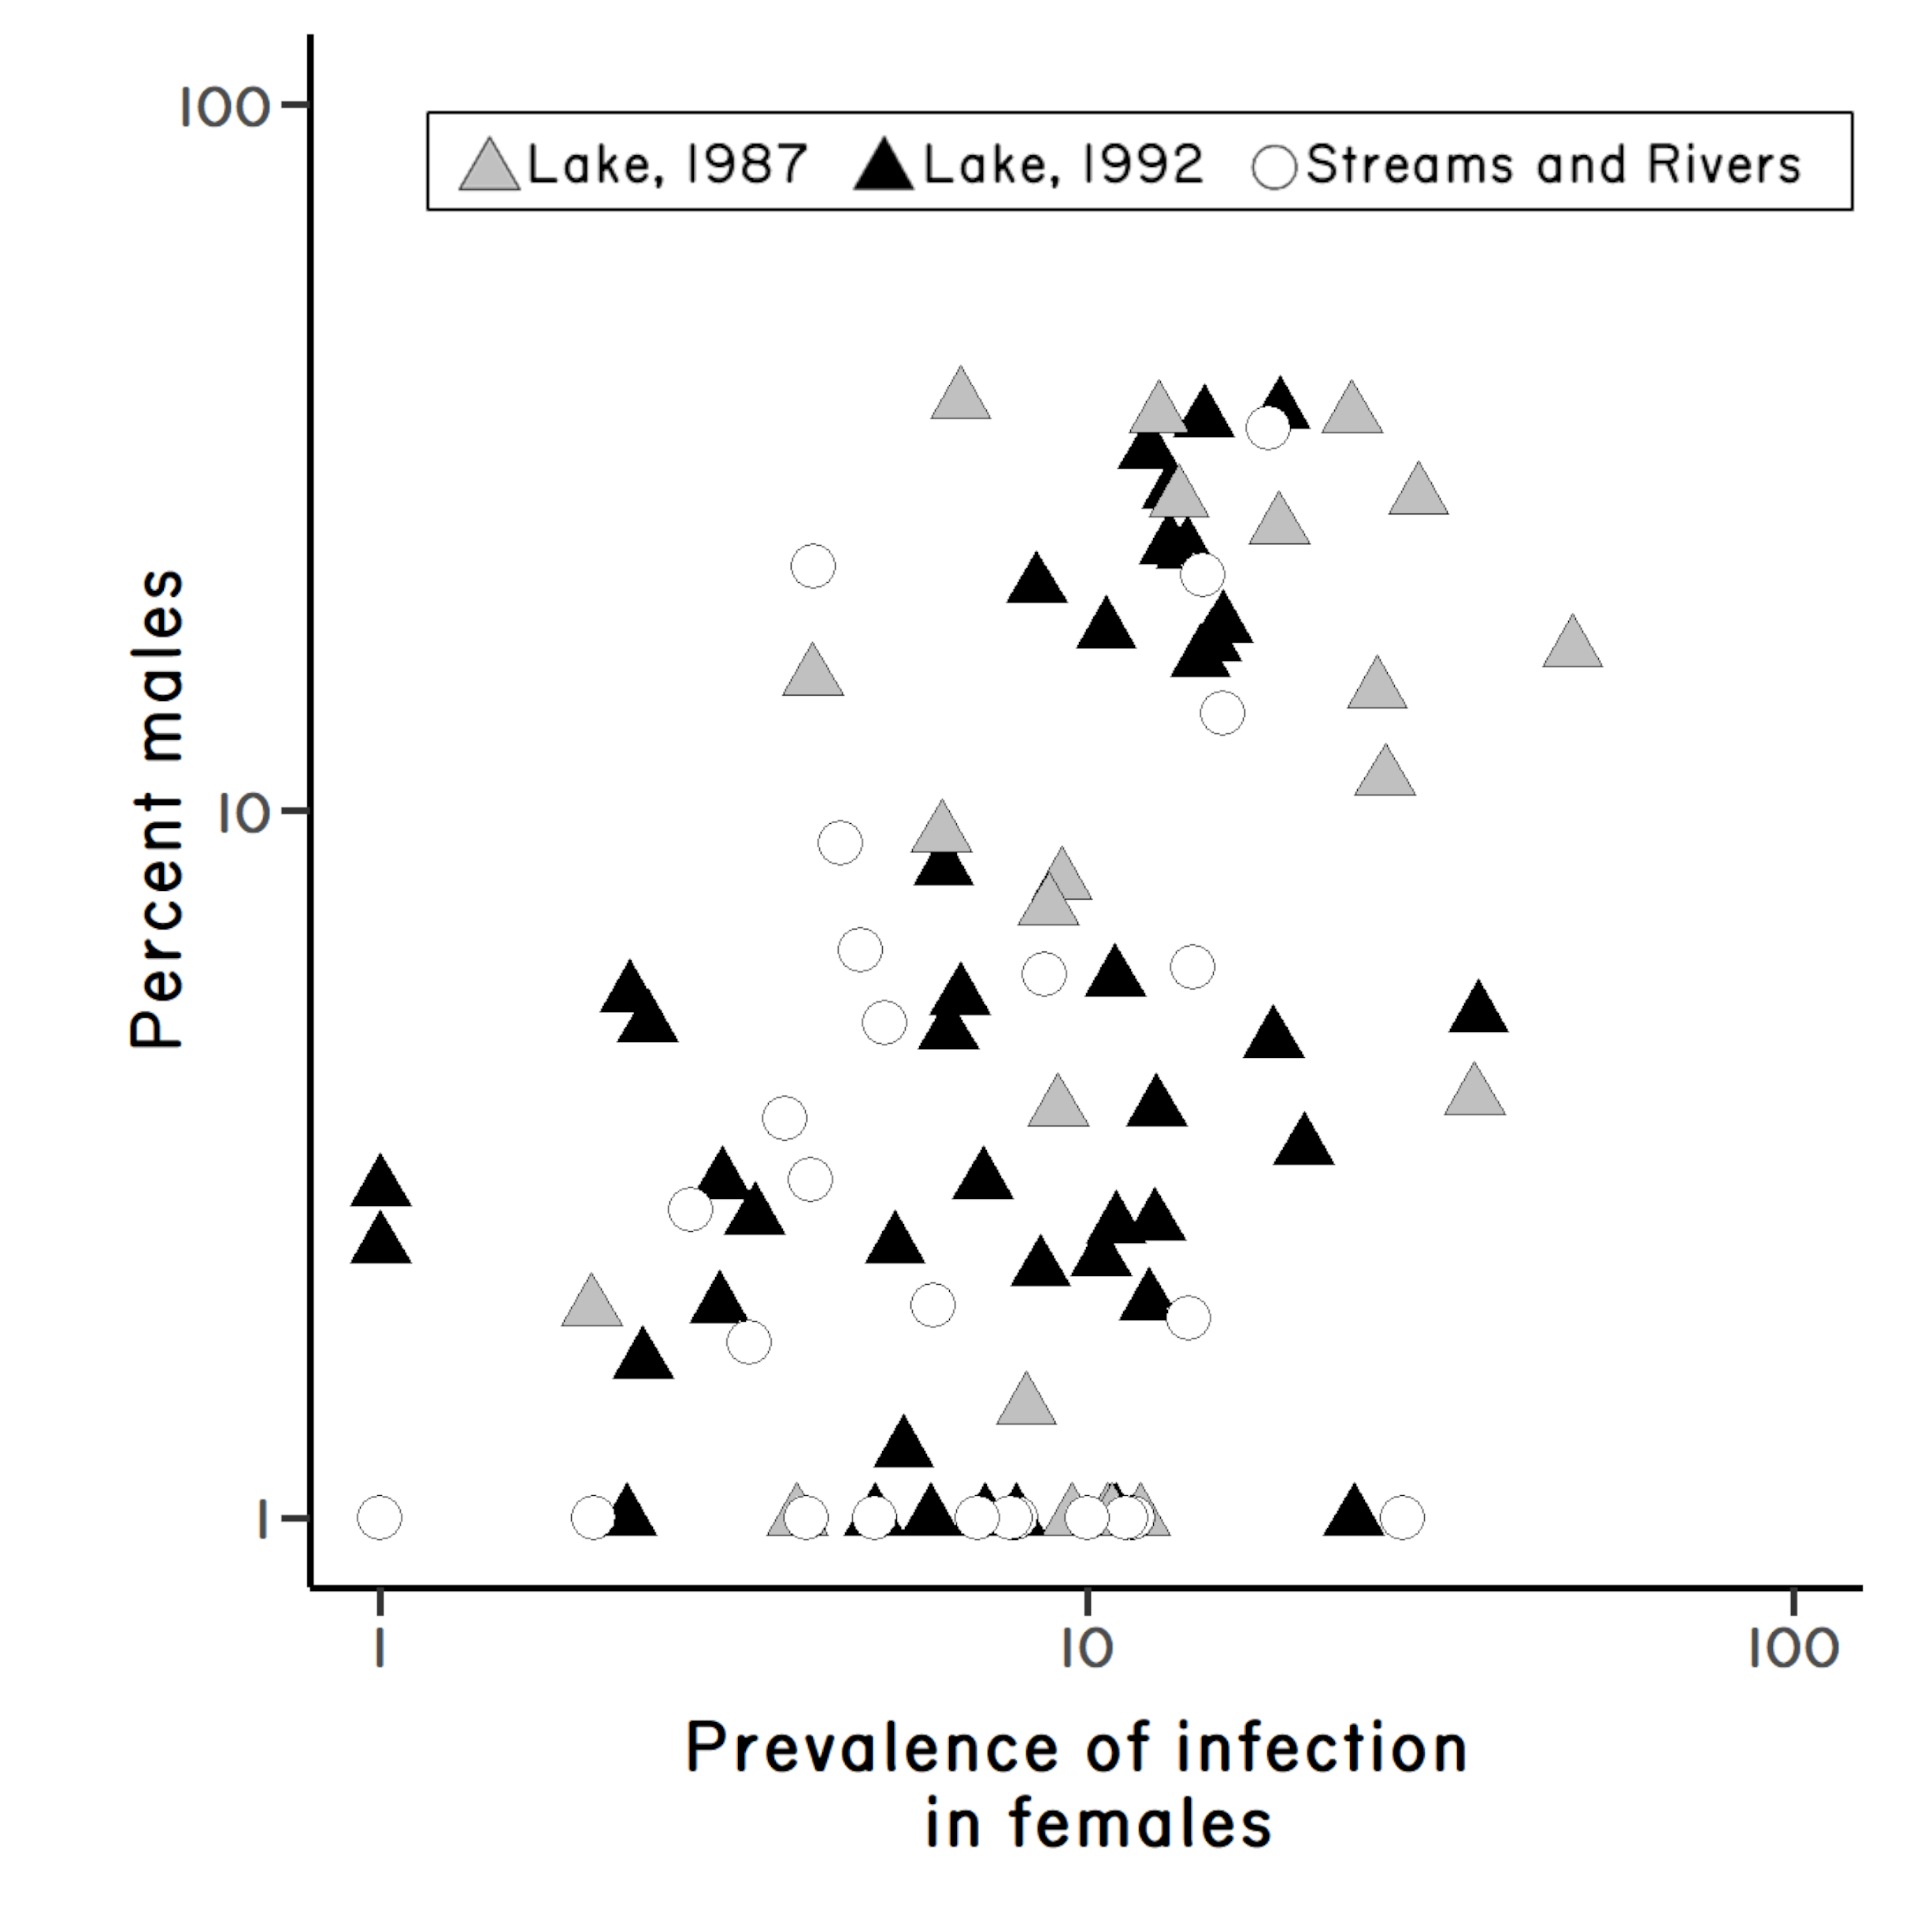
\includegraphics[width=0.6\textwidth,height=\textheight]{images/fig3-5_hr.png}

}

\caption[Results from surveys of New Zealand lakes and streams showing
percent males against the prevalence of female infection by all species
of trematodes]{\label{fig-3-5}Results from surveys of New Zealand lakes
and streams showing percent males against the prevalence of female
infection by all species of trematodes. Note the upper left side of the
graph. There are no highly sexual populations where parasites are rare
or absent, which suggests that asexuals have replaced sexuals were
parasite-mediated selection is weak. This result is consistent with
Lloyd's prediction given in Chapter~\ref{sec-eco-hyp}. Circles represent
stream populations (\citeproc{ref-lively1987a}{Lively 1987}) plus two
river samples. Gray triangles represent lake populations
(\citeproc{ref-lively1987a}{Lively 1987}). Black triangles represent
lake and tarn populations (\citeproc{ref-lively1992a}{Lively 1992}). The
correlation is positive and statistically significant.}

\end{figure}%

\begin{figure}

\centering{

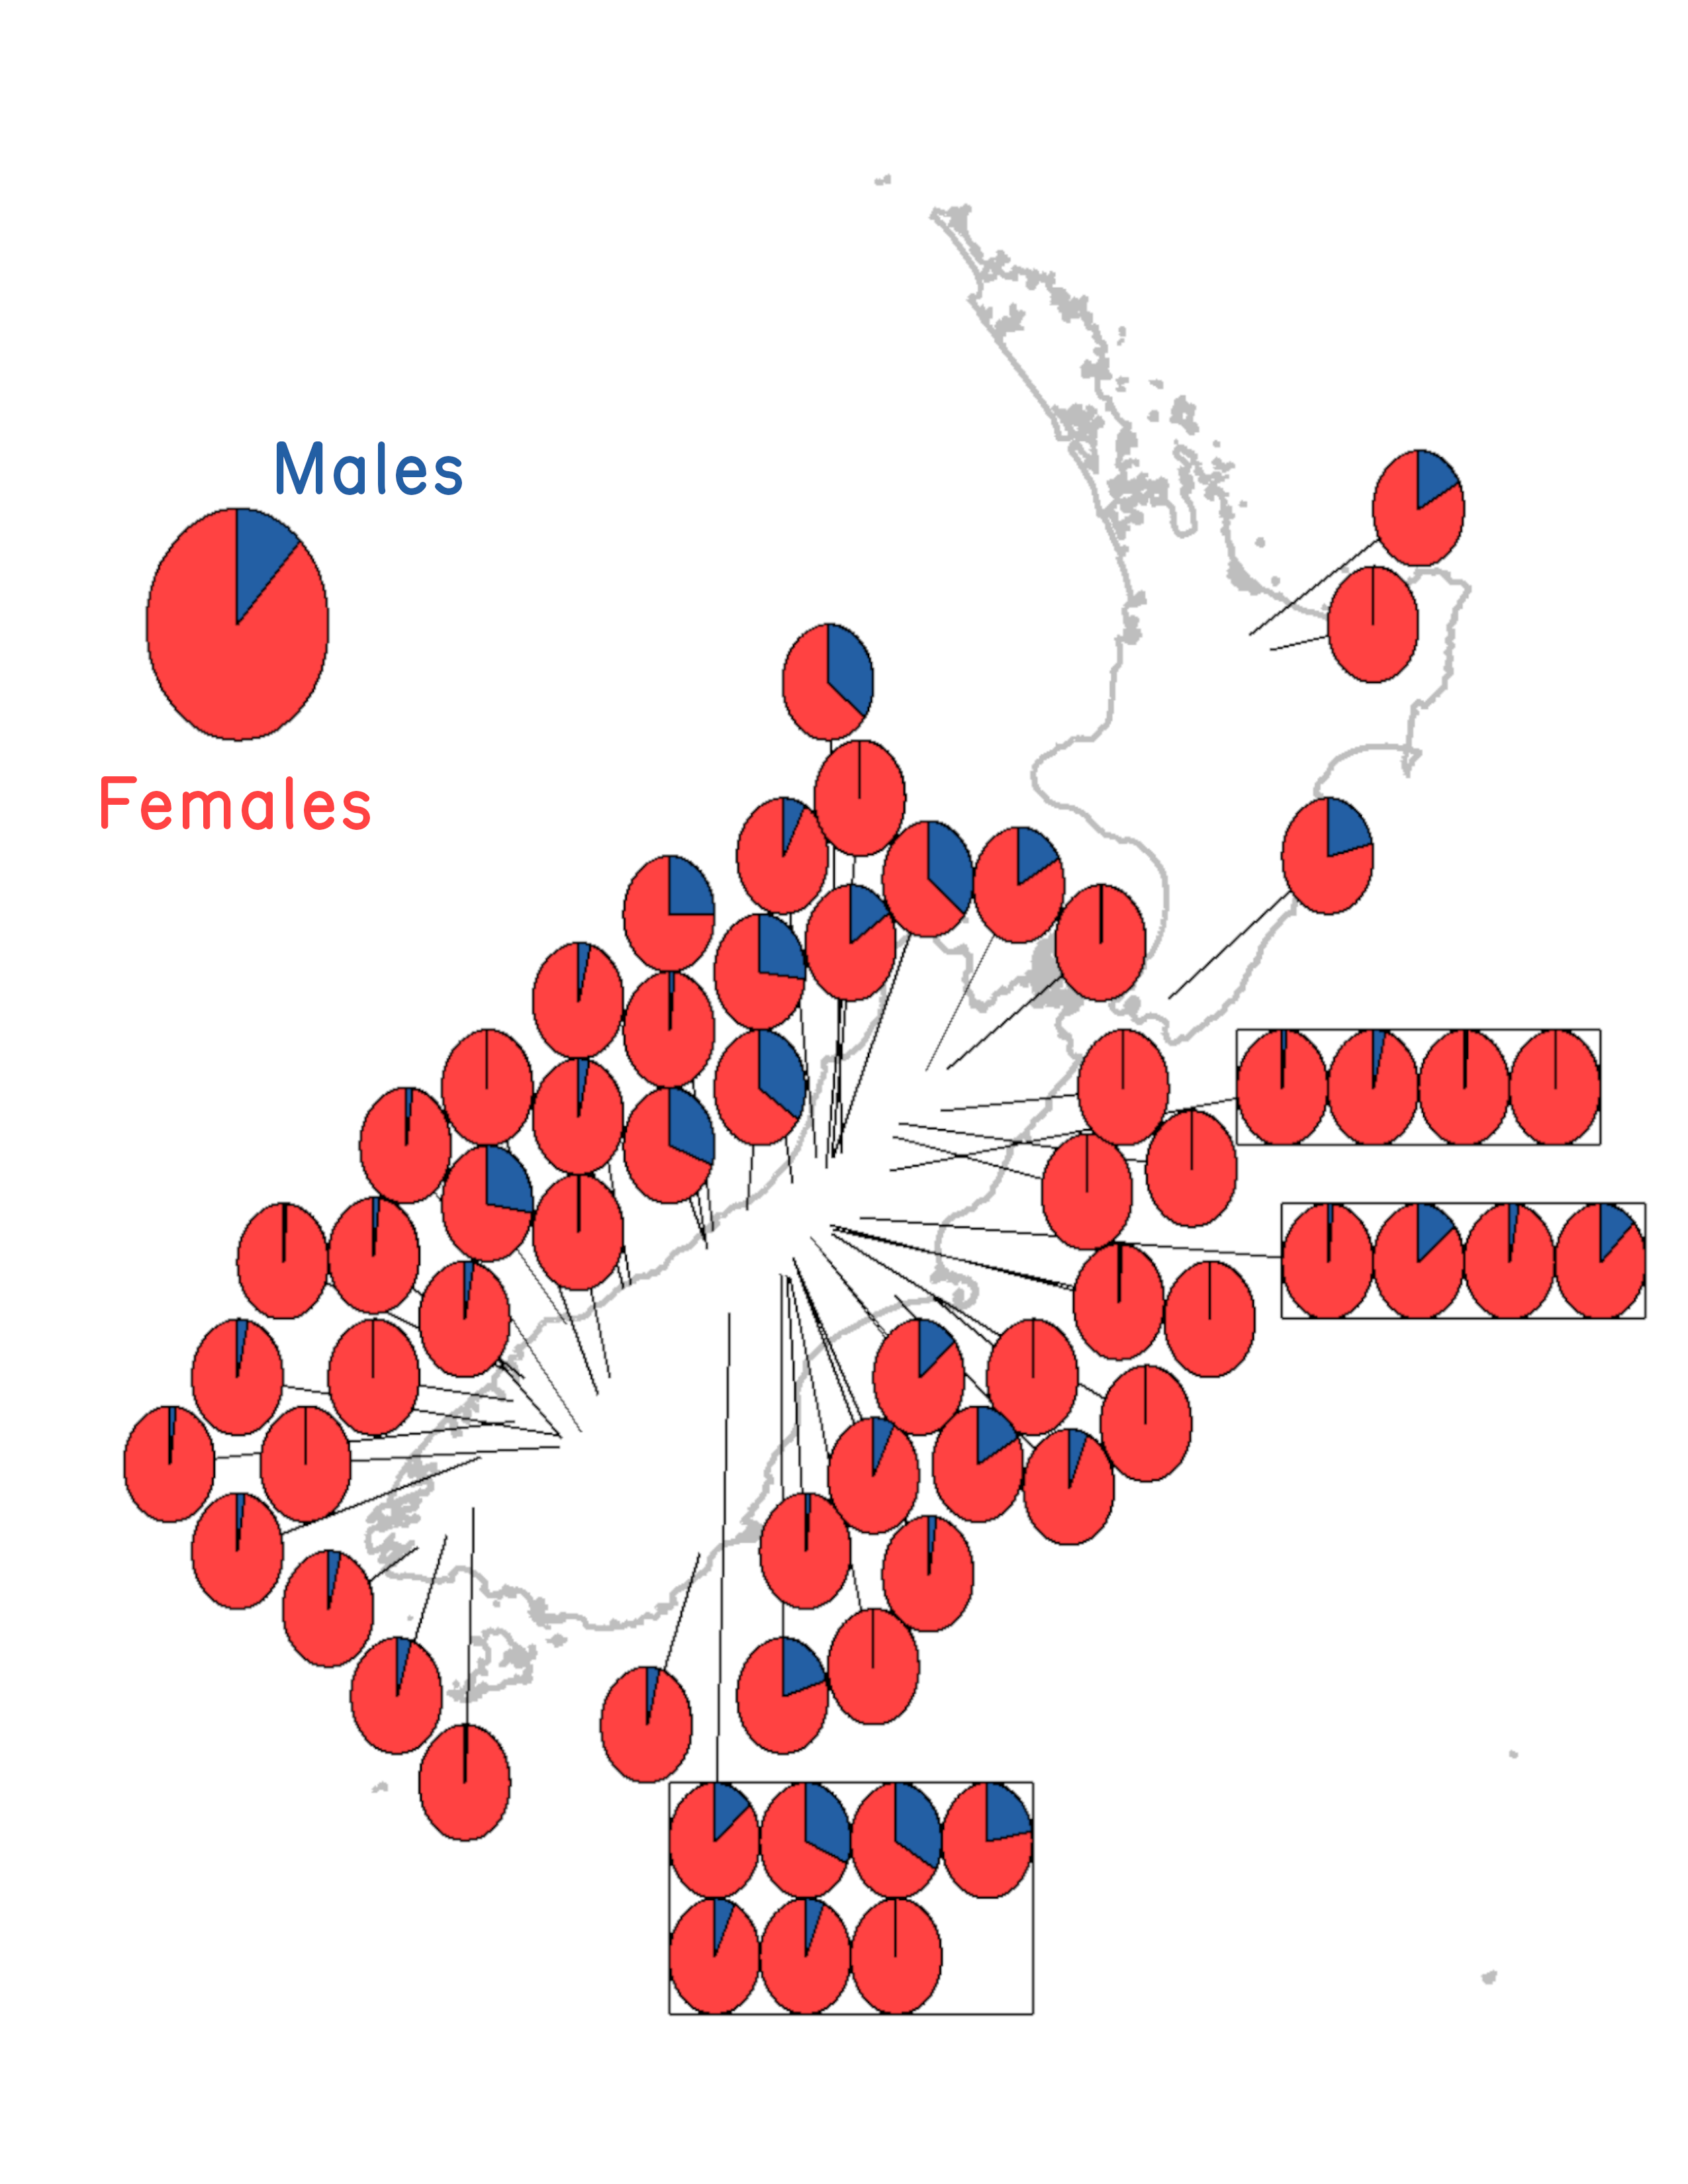
\includegraphics[width=0.6\textwidth,height=\textheight]{images/fig3-6_hr.png}

}

\caption[Distribution of male and female \emph{Potamopyrgus antipodarum}
across New Zealand]{\label{fig-3-6}The distribution of male and female
\emph{Potamopyrgus antipodarum} across New Zealand. The percentage of
males is given in blue; the percentage of females is given in red. Pie
charts enclosed in boxes are for lakes and tarns that are very close
together. The large pie on the left-hand side shows the average
frequencies of males and females across all samples. (Redrawn from
\citeproc{ref-lively1992a}{Lively 1992}.)}

\end{figure}%

These results suggested that parasite-mediated selection might
contribute to the persistence of sex in mixed populations of sexual and
asexual snails. It is of particular interest, perhaps, to note that
there are no populations with a high proportion of males in samples
where parasites were rare or absent (Figure~\ref{fig-3-5}). This finding
is consistent with David Lloyd's (\citeproc{ref-lloyd1980a}{1980}) 1980
prediction that asexuals should dominate in populations ``with a
relaxation of biological hostility'' (see above). But the results are
messy.

There are several reasons for why the results might be expected to be
messy. One is that prevalence of infection might not give a good
estimate of the strength of parasite-mediated selection
(\citeproc{ref-lively2001a}{Lively 2001}). For example, infected snails
might die at a faster rate than uninfected snails because of the
energetic demands of infection. In addition, infected snails are more
likely than uninfected snails to forage after sunrise, which exposes
them to predation by their final hosts, ducks
(\citeproc{ref-levri2000a}{Levri \& Fisher 2000};
\citeproc{ref-levri1996a}{Levri \& Lively 1996}). Prevalence of
infection might also fluctuate over time as the genetic diversity in the
host population changes and/or as the final hosts move among locations.
We now know that the prevalence of infection varies greatly among years
and among sites in the same lake (\citeproc{ref-gibson2016a}{Gibson
\emph{et al.} 2016}). Thus, detecting a significant correlation between
sex and infection could be dicey, even if parasites were solely
responsible for the short-term maintenance of sex in mixed
populations.\footnote{Using computer simulations, we recently found that
  detecting a significant positive correlation between clonal diversity
  and infection prevalence would only be expected in a fraction of
  parameter space, even when parasites were solely responsible for the
  maintenance of diversity (\citeproc{ref-lively2021a}{Lively \emph{et
  al.} 2021}).}

Along these lines, many of the points in Figure~\ref{fig-3-5} represent
a single sample taken at one site at one point in time. This limitation
likely introduces ``noise'' into the data, especially for samples where
parasites are only periodically common. For this reason, Jukka Jokela
and I selected 20 of the best sampled lakes from the data set given in
Figure~\ref{fig-3-5}.\footnote{In this smaller sample of 20 lakes, the
  correlation between male frequency and infection prevalence was
  positive but not statistically significant.} We resampled all 20 lakes
10 -- 15 years after my original samples. We found that prevalence of
infection was highly correlated between sample periods as was male
frequency (\citeproc{ref-lively2002a}{Lively \& Jokela 2002}). We then
averaged the data for each lake under the assumption that the averages
would better represent both the frequency of males and the prevalence of
infection for each lake. With these data, the correlation between male
frequency and infection prevalence was both positive and
significant.\footnote{\(r = 0.47\); \(P = 0.04\) for
  log\textsubscript{10} transformed data; \(N = 20\).}

None of this is meant to imply proof of the Red Queen Hypothesis or that
density dependence and random environmental change are not relevant for
a full understanding of the problem.\footnote{I think density dependence
  is critically important. Disease transmission is certainly density
  dependent (\citeproc{ref-anderson1979a}{Anderson \& May 1979};
  \citeproc{ref-may1979a}{May \& Anderson 1979}). Virulence may also be
  density dependent (\citeproc{ref-bell2006a}{Bell \emph{et al.} 2006};
  \citeproc{ref-lively1995a}{Lively \emph{et al.} 1995};
  \citeproc{ref-lively2006a}{Lively 2006}). Habitat partitioning may
  also play a role in the distribution of sexual females among
  depth-stratified habitats (\citeproc{ref-negovetic2001a}{Negovetic \&
  Jokela 2001}).} But the results do imply that the Red Queen Hypothesis
was (and still is) worthy of further study.

\section{Summary}\label{summary-2}

\begin{enumerate}
\def\labelenumi{\arabic{enumi}.}
\tightlist
\item
  The co-occurrence of discrete morphs is inherently interesting to
  evolutionary biologists. Genetic diversity is also inherently
  interesting.
\item
  Some populations of the New Zealand freshwater snail,
  \emph{Potamopyrgus antipodarum}, contain both sexual and asexual
  females. Other populations are mostly or completely parthenogenetic.
  This makes the snail a very useful natural system for contrasting
  alternative hypotheses for the maintenance of sexual reproduction.
\item
  The prevalence of sterilizing trematode larvae is a better predictor
  sexual reproduction in the snail than habitat (lakes versus streams),
  thus favoring the Red Queen Hypothesis over the alternative ecological
  hypotheses.
\item
  Comparing the \emph{a priori} predictions of multiple working
  hypotheses can be helpful to evaluate competing ideas. Field studies
  of natural systems may be required to fully understand why
  cross-fertilization is so common.
\end{enumerate}

\section{Appendix: A Model of Phenotypic Plasticity}\label{sec-app-3}

As part of my dissertation research, I constructed a game-theoretic
model of selection on three strategies:

\begin{itemize}
\tightlist
\item
  canalized development into a high-fecundity morph,
\item
  canalized development to a low-fecundity, predation-resistant morph,
\item
  induced development into the low fecundity defended morph in the
  presence of predators.
\end{itemize}

The model examined evolutionary stability for a range of frequencies for
two patches (high predation risk and low predation risk) across a range
of values for the accuracy of the cue predicting future predation risk
(\citeproc{ref-lively1986a}{Lively 1986a}).

An example of the output is shown below. The results show that any of
the three strategies can be an ESS in part of the parameter
space.\footnote{``Parameter space'' represents all possible combinations
  of variables as defined by the model. In Section~\ref{sec-app-3},
  different strategies are favored for different combinations of
  variables (i.e., different parts of the parameter space).} High
reliability of the cue and intermediate patch frequencies favor the
plastic strategy. Genetic polymorphism is expected under a relatively
narrow set of conditions. Mixtures of constitutive and plastic
strategies can also be stable. Note that changing the patch frequencies
leads to evolutionary change. For example, reducing the frequency of the
low-risk patch can lead to a selective sweep (arrow a). It can also lead
to the evolution of plasticity (arrow b) and the evolution of canalized
development (arrow c). Increasing the accuracy of the cue can also lead
to the evolution of plasticity. It might be especially interesting to
note that the trajectory of arrow b would give the appearance of
saltatory change followed by stasis (i.e., punctuated equilibrium)
(\citeproc{ref-levinton1988a}{Levinton 1988}). Also note that the
conditions for a genetic polymorphism are relatively narrow. Redrawn
from Lively (\citeproc{ref-lively1999b}{1999a}) assuming a small cost to
plasticity.

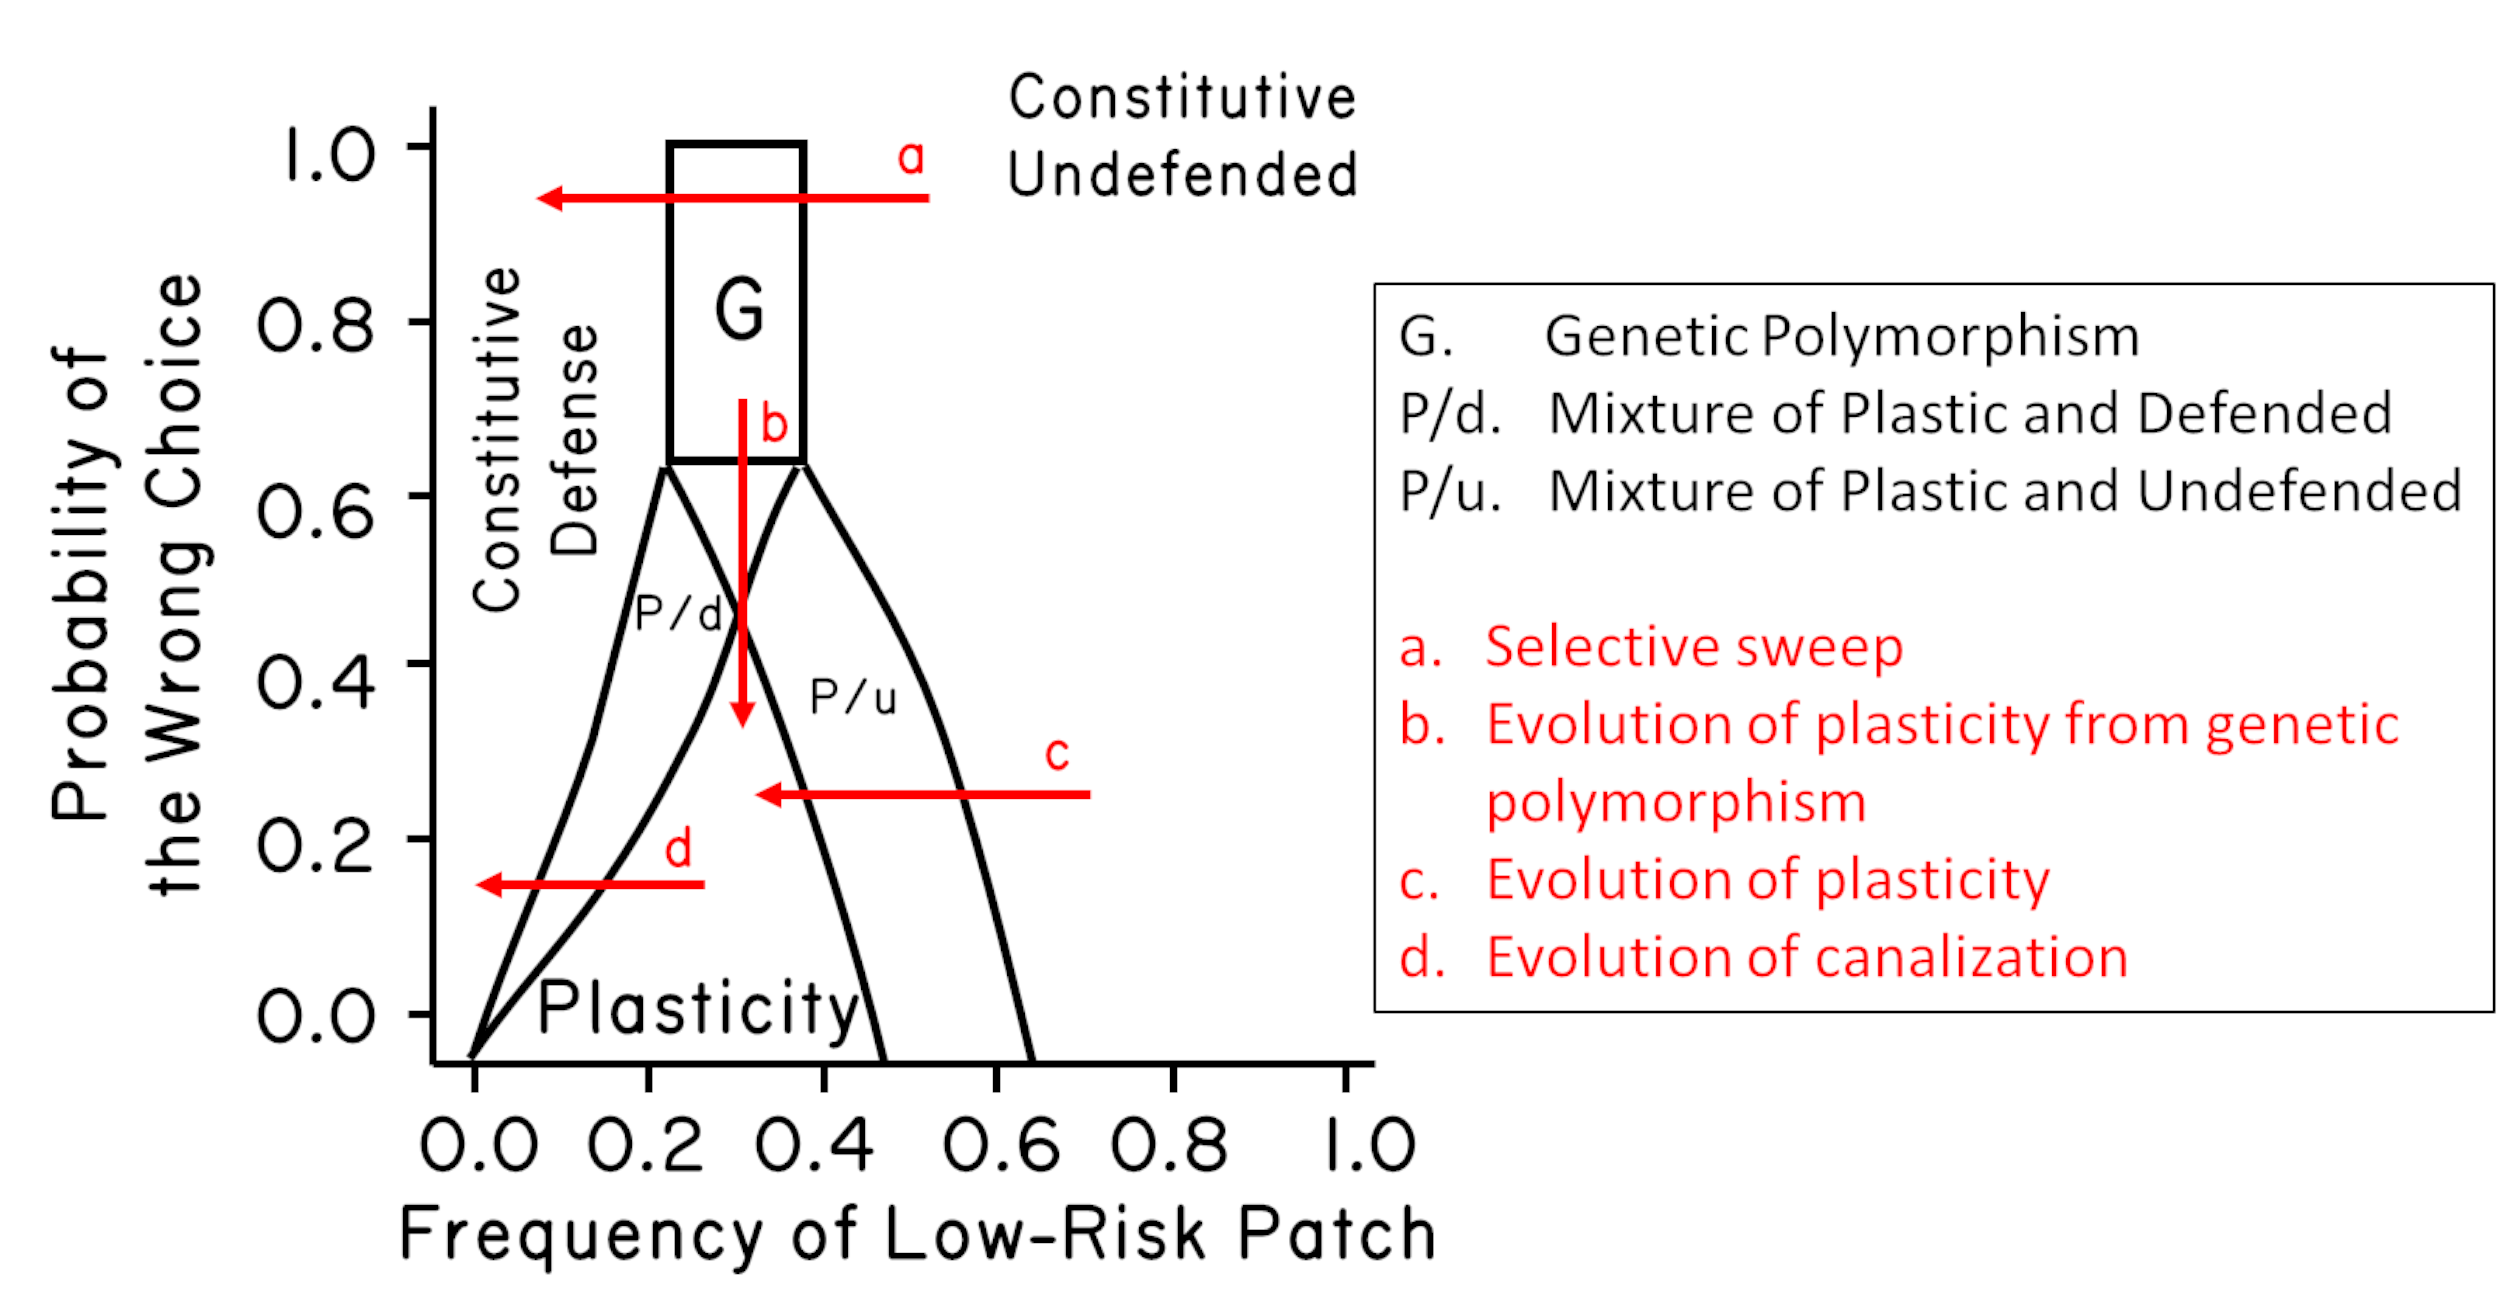
\includegraphics{images/fig3-7_hr.png}

\bookmarksetup{startatroot}

\chapter{Self- / Non-Self-Recognition and Local
Adaptation}\label{sec-self-non}

\begin{center}
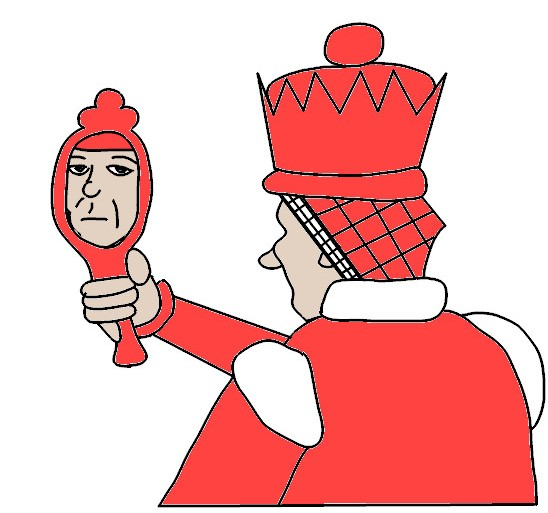
\includegraphics[width=0.5\textwidth,height=\textheight]{images/fig4-1.jpeg}
\end{center}

One way to falsify the Red Queen is to experimentally show that the
expectations of the hypothesis are not met. One expectation is that
parasites would quickly become adapted to infecting their local host
populations. Here is the logic. If parasites are closely tracking common
host genotypes in their local (sympatric) populations, then they should
be better, on average, at infecting sympatric hosts than foreign
(allopatric) hosts. If this is not the case, then parasites would seem
unlikely (at least to me) to be a factor selecting for sexual
reproduction.

I am often asked why we would expect the parasites to be better at
infecting their local hosts instead of the opposite. Why shouldn't hosts
evolve to be more resistant to their local parasites than to allopatric
parasites? It is a fair question. One common answer is that parasites
are locally adapted to host populations because they have faster
generation times. But that cannot be the whole answer. Theory has shown
that parasites can be locally adapted even when there is no
generation-time asymmetry (\citeproc{ref-gandon2002a}{Gandon \&
Michalakis 2002}; \citeproc{ref-lively1999a}{Lively 1999b}). Instead, I
think the answer has more to do with the underlying genetic basis for
infection.

What, then, is the genetic basis for infection? This was unknown, but I
was assuming that all animal hosts have a self- / non-self-recognition
system, such that they can detect foreign tissues (e.g., parasites or
tissue grafts) that do not match their own. Sponges, for example, accept
tissue grafts from self, but reject grafts from unrelated individuals of
the same species (review in \citeproc{ref-gaino1999a}{Gaino \emph{et
al.} 1999}). This ability to reject foreign tissues seems widely
conserved (\citeproc{ref-buss1990a}{Buss 1990}). I was also assuming
that the self- / non-self-recognition system is genetically variable and
that different host genotypes would dominate in different populations.
Parasite genotypes that match the most common local host genotypes would
be favored by natural selection, and these parasite genotypes should
increase in frequency. This should lead to local adaptation by the
parasites. Fortunately, one can test for local adaptation using
reciprocal cross-inoculation experiments.

\section{Experimental Studies of Local
Adaption}\label{experimental-studies-of-local-adaption}

While I was still a post-doc in New Zealand, I set up two reciprocal
cross-inoculation experiments to test for local adaptation by the
parasites. I knew from my field surveys that one species of sterilizing
trematode was especially common in lake populations of the snail. This
species was not formally described, but Jan McKenzie sent it to a
trematode expert in France, who thought it belonged in the genus
\emph{Microphallus}; hence I will refer to it as \emph{Microphallus}
sp.\footnote{The trematode worm was not formally described until 30
  years later (\citeproc{ref-blasco-costa2019a}{Blasco-Costa \emph{et
  al.} 2019}). As it turns out, it belongs in the genus
  \emph{Atriophallophorus}, rather than \emph{Microphallus}, and it was
  very appropriately named after Mike Winterbourn: \emph{A.
  winterbourni}. But I am going to call it \emph{Microphallus} in this
  book, as that is what we called it in our early papers.} The life
cycle of \emph{Microphallus} turns out to be especially crucial to the
story. The adult worms are tiny simultaneous hermaphrodites that live in
the intestines of ducks. They cross-fertilize and produce eggs that are
shed with the duck feces into the environment. In most trematodes, the
eggs normally hatch in water, thereby releasing a swimming larval stage
(miracidia), which actively swims to and penetrates the body of snails.
This is the case for the trematodes that cause the human disease,
Schistosomiasis. But, in this New Zealand species of
\emph{Microphallus}, the eggs hatch not in the environment but rather
after being ingested by snails. The larvae then penetrate the snail from
the inside. If the snail's immune system does not recognize the larvae
as foreign tissue, the larvae reproduce asexually, producing several
hundred cysts (metacercaria) in the snail. These cysts completely
replace the reproductive tissue in both males and females. Infected
snails are sterilized (Figure~\ref{fig-4.1}; Figure~\ref{fig-4.2}).

\begin{figure}

\centering{

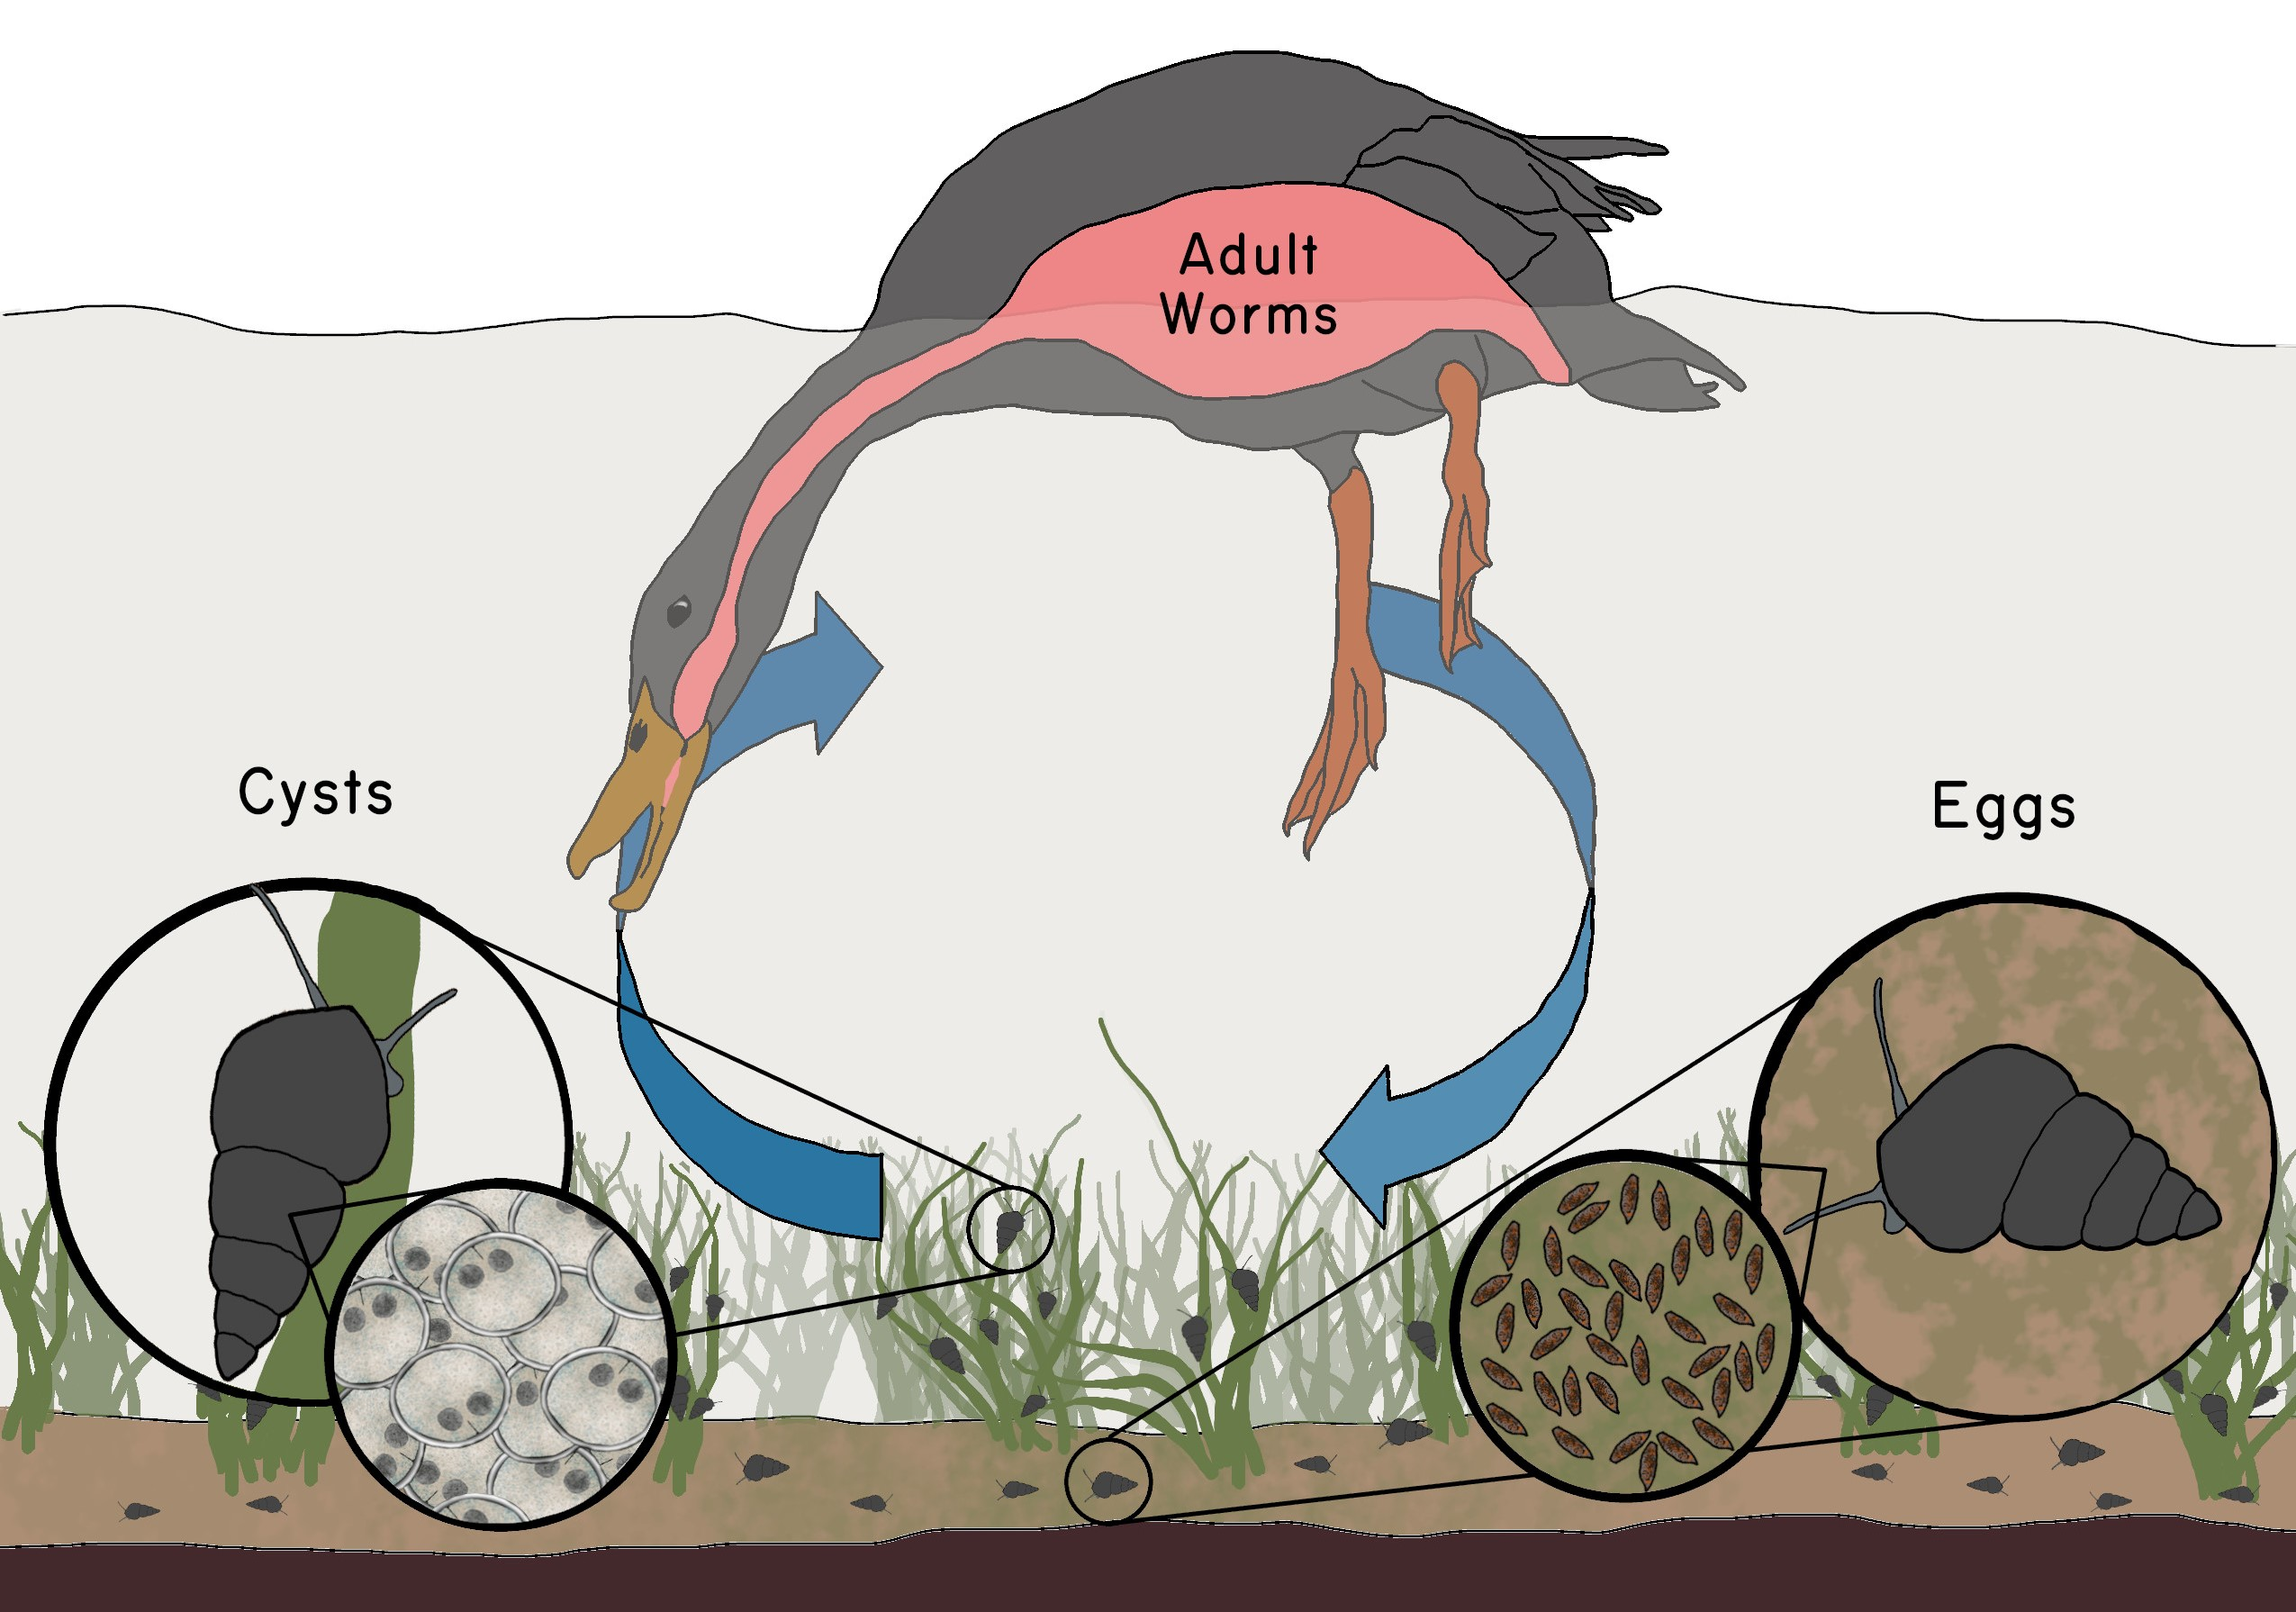
\includegraphics[width=0.7\textwidth,height=\textheight]{images/fig4-2.jpeg}

}

\caption[The life cycle of the trematode
\emph{Microphallus}]{\label{fig-4.1}The life cycle of the trematode
\emph{Microphallus}. The adult worms live in the intestines of waterfowl
and wading birds (black stilts). They produce cross-fertilized eggs,
which are released into lakes and streams with the bird's feces. The
eggs hatch following ingestion by snails. Infection results in the
asexual production of hundreds of cysts (called metacercaria). These
cysts ``hatch'' and mature following ingestion by ducks, thus completing
the life cycle. Drawing by Zoe M Dinges.}

\end{figure}%

\begin{figure}

\centering{

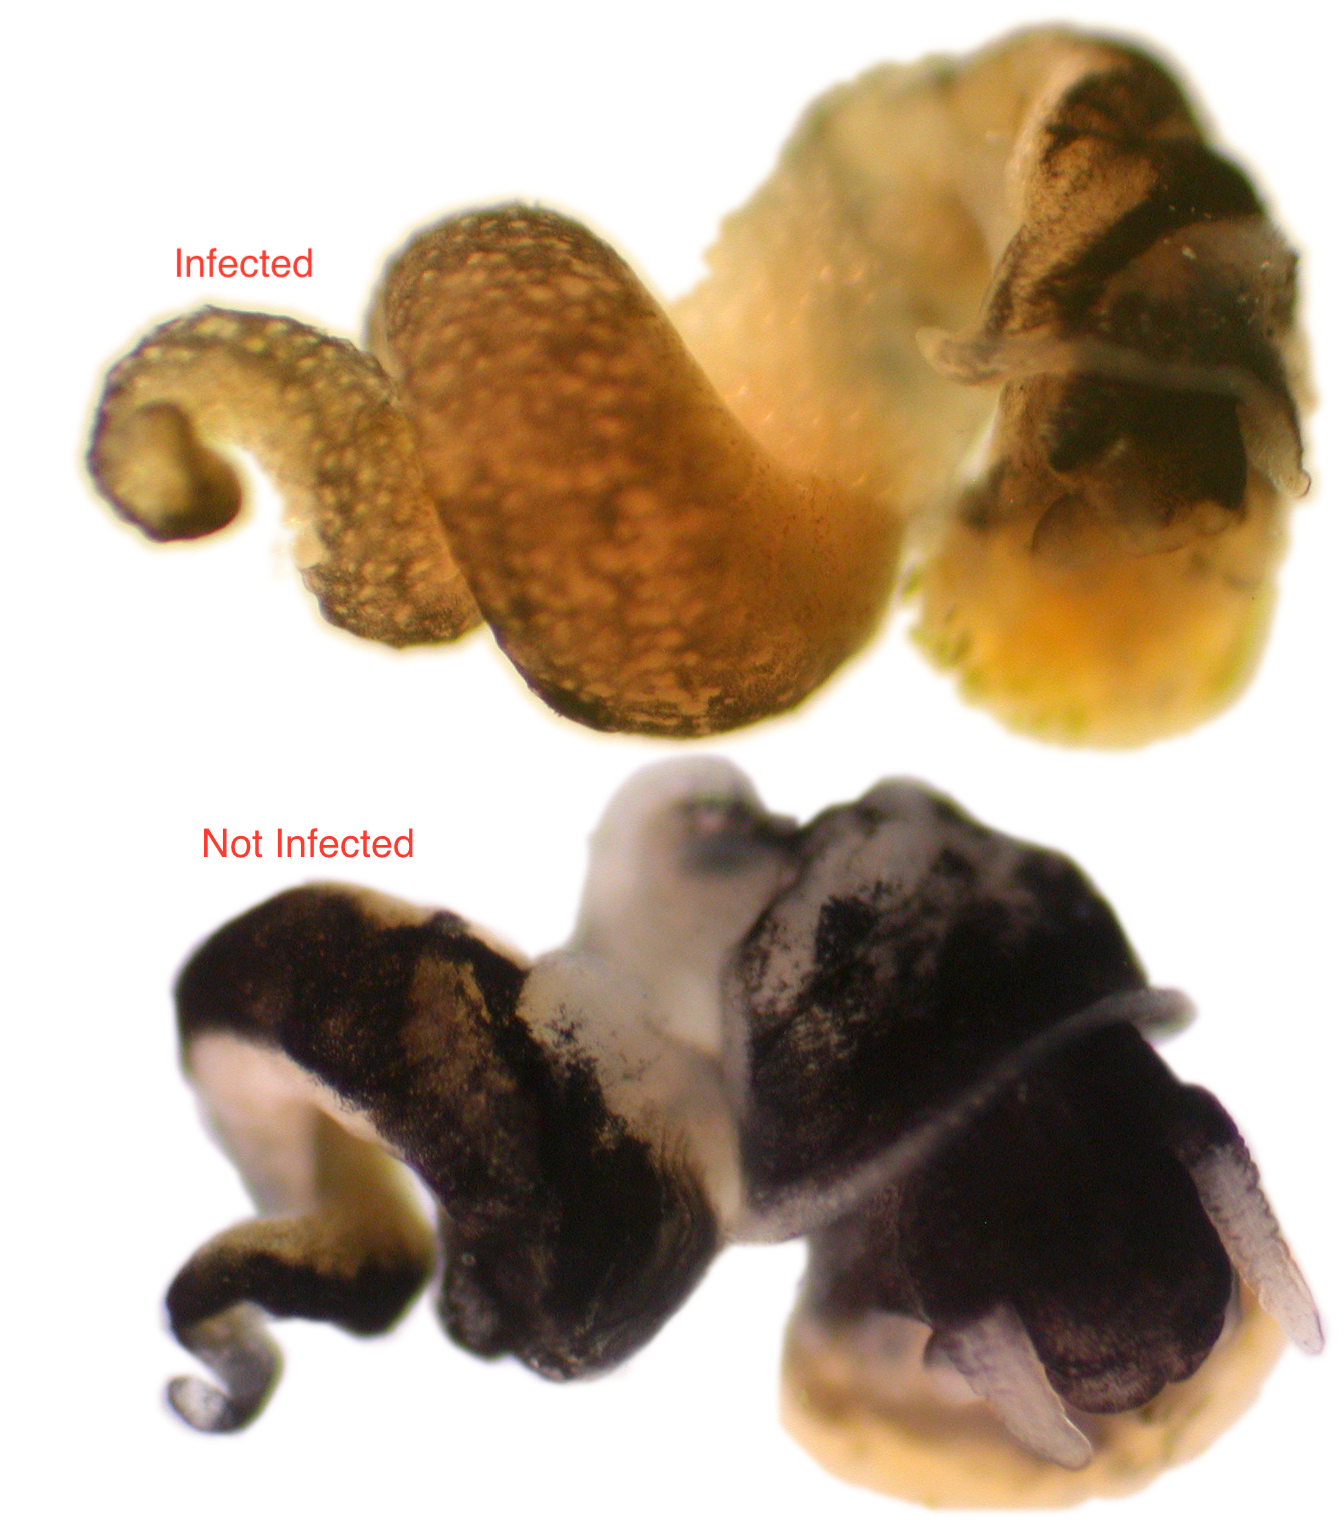
\includegraphics[width=0.6\textwidth,height=\textheight]{images/fig4-3.jpg}

}

\caption[Infected female (top) and uninfected female (bottom) of
\emph{P. antipodarum}]{\label{fig-4.2}\textbf{Photo Credit: © Gabe Harp.
Used by permission.} Infected female (top) and uninfected female
(bottom) of \emph{P. antipodarum}. The snails had been removed from
their shells. The golden cysts in the infected female (top) are
\emph{Microphallus} metacercaria. The white tissue of the uninfected
female (bottom) is ovary.}

\end{figure}%

I set up an experiment in which I exposed snails from two different
lakes to \emph{Microphallus} eggs from both lakes. One lake was on the
east side of the Southern Alps (Lake Alexandrina), and the other lake
was on the west side of the alps (Lake Mapourika). I reasoned that gene
flow between the two lakes was likely to be very low, so it seemed
unlikely that gene flow could swamp out parasite-mediated selection (if
present). But to get the eggs, I had to first complete the life cycle of
the parasite in the lab. This had never been done. Eventually, I took
the advice of Dr.~David Blair, a friend and parasitologist at the
University of Canterbury: I fed the cysts to lab mice. I then collected
the mouse poo, washed it, and fed the slurry to snails. It seemed very
unlikely to work, as ducks (not mice) were the vertebrate host, but I
tried it anyway. It worked! I was able to experimentally infect snails
in the lab. And, amazingly, the parasites from both lake populations
were much more infective to snails from their same lake
(Figure~\ref{fig-4.3}). In other words, the \emph{Microphallus}
parasites were locally adapted (\citeproc{ref-lively1989a}{Lively
1989}). There was no reason based on this experiment to discard the Red
Queen.

\begin{figure}

\centering{

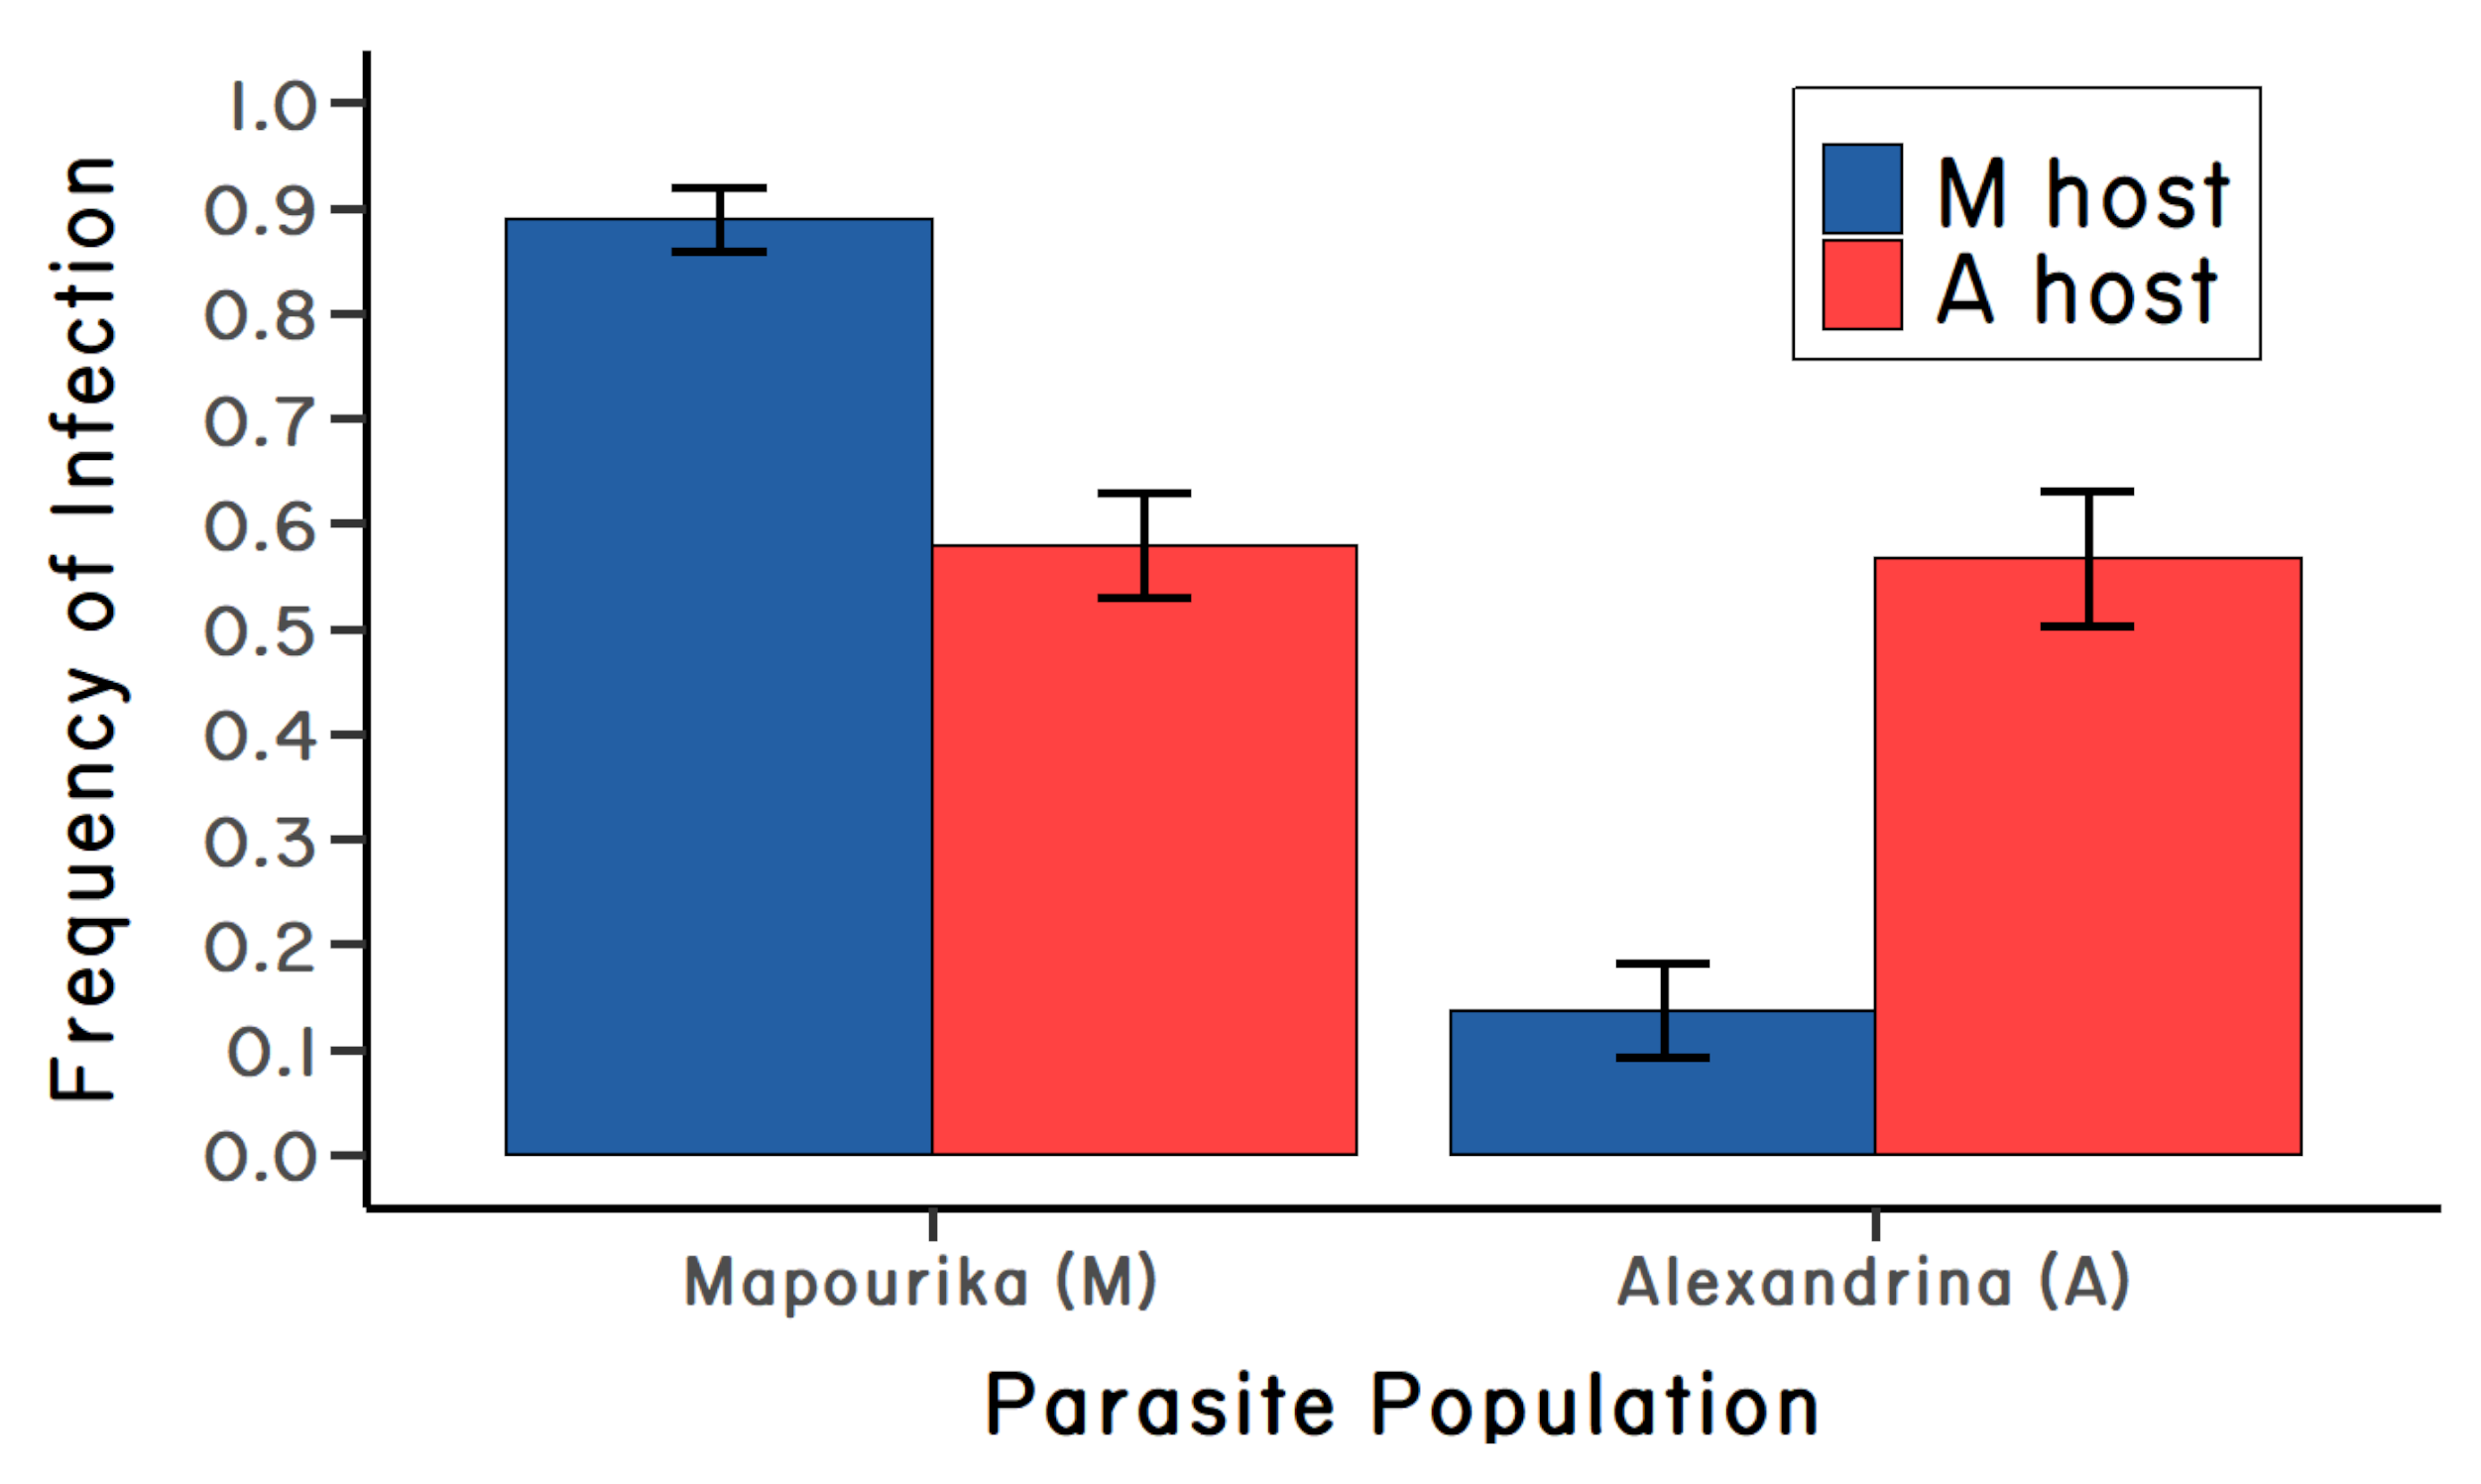
\includegraphics[width=0.75\textwidth,height=\textheight]{images/fig4-4.png}

}

\caption[Results of the first reciprocal cross-inoculation
experiment]{\label{fig-4.3}Results of the first reciprocal
cross-inoculation experiment. The vertical bars show one SE of the mean.
Redrawn from Lively (\citeproc{ref-lively1989a}{1989}).}

\end{figure}%

On the other hand, there were only two lakes in the experiment, so it
was unclear if local adaptation was generally true for
\emph{Microphallus}. So, I repeated the experiment
(\citeproc{ref-lively1989a}{Lively 1989}). This time I sampled three
lakes, all on the west side of the alps. Two of the lakes were less than
ten kilometers apart (Lakes Mapourika and Wahapo). The third lake (L.
Paringa) was about 100 kilometers south of Lake Mapourika (see map in
Lively (\citeproc{ref-lively1989a}{1989})). It seemed likely to me that
parasite gene flow would be very high between Mapourika and Wahapo,
which might reduce or eliminate local adaptation in the parasite. I
exposed snails from all three lakes to parasites from each of the three
lakes in a fully reciprocal cross-inoculation experiment. Again, the
results were very clear: the parasites (following passage through mice)
from all three lakes were more infective to host snails from the same
lake (\citeproc{ref-lively1989a}{Lively 1989}). And, to my surprise, the
distance between lakes did not matter to the strength of local
adaptation (Figure~\ref{fig-4.4}). Taken together the results from two
independent experiments showed strong adaption by parasites to local
populations of their snail host. The results also suggested a genetic
basis for host resistance and parasite infectivity, which is a crucial
assumption of the Red Queen Hypothesis. Finally, the pattern of local
parasite adaptation in the snail-trematode system would be found to be
very robust in experiments conducted by me and my students after I moved
to Indiana University (Figure~\ref{fig-4.5}).

\begin{figure}

\centering{

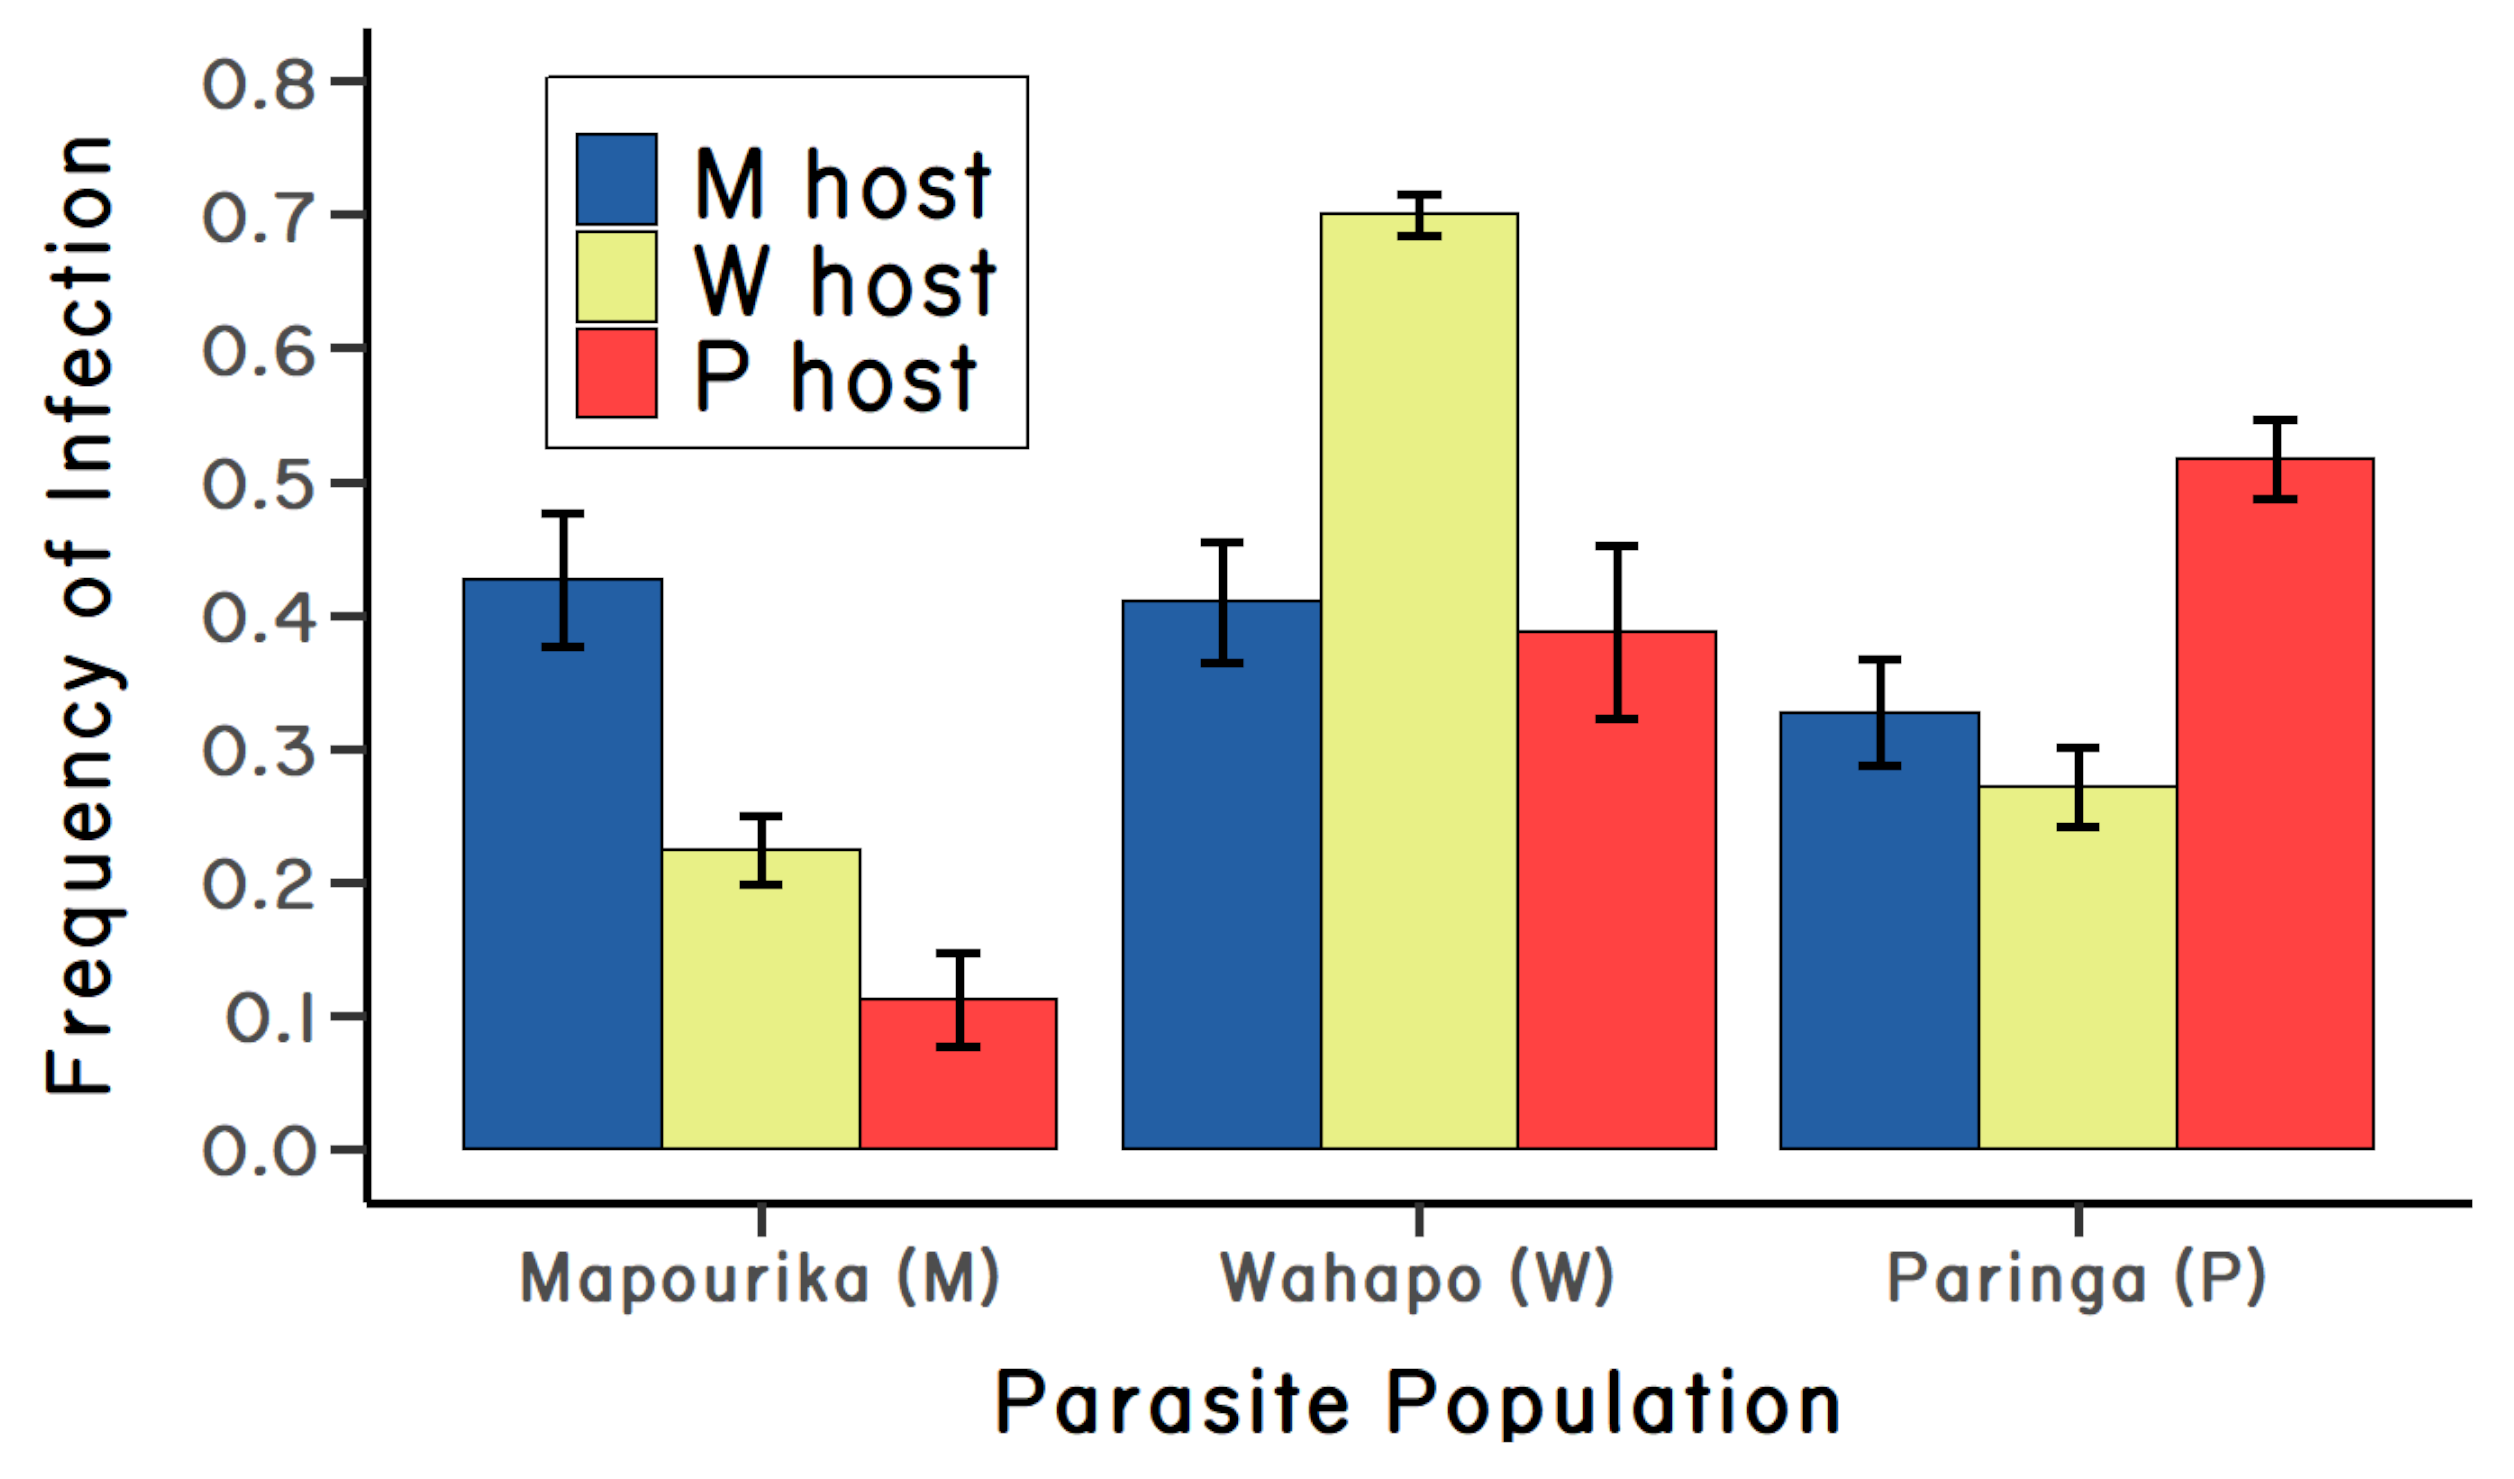
\includegraphics[width=0.75\textwidth,height=\textheight]{images/fig4-5.png}

}

\caption[Results of the second reciprocal cross-inoculation
experiment]{\label{fig-4.4}Results of the second reciprocal
cross-inoculation experiment. Vertical bars show one SE of the mean.
Redrawn from Lively (\citeproc{ref-lively1989a}{1989}).}

\end{figure}%

Does local adaptation by parasites mean that hosts are losing? If so,
are hosts maladapted, as often claimed? No and no. The host population
is evolving as fast as it can to resist infection by local parasites,
and local parasites are tracking the genetic changes in their host
populations (with a time lag). This tracking by parasites results in
local adaption. In computer simulations, the change in host mean fitness
oscillates over time from positive to negative and back. Parasite mean
fitness also oscillates from positive to negative, but it is 180 degrees
out of phase with the host (\citeproc{ref-lively1999a}{Lively 1999b};
\citeproc{ref-lively2022a}{Lively \& Wade 2022}). Thus, local parasite
adaptation does not necessarily mean that the hosts are losing.
Sometimes the host is winning (positive change in mean fitness) and the
parasite is losing (negative change in mean fitness), and sometimes the
host is losing and the parasite is winning. Over time, the average
change in mean fitness for both species is zero.

My early results on local adaptation along with the results of Parker
(\citeproc{ref-parker1985a}{1985}) and Ebert
(\citeproc{ref-ebert1994a}{1994}) convinced me that host-parasite
coevolution was interesting, whether or not it could explain
sex.\footnote{Dieter Ebert showed that parasites of \emph{Daphnia} were
  locally adapted for both infectivity and transmission, which was a
  major advance.} In addition, May and Anderson
(\citeproc{ref-may1983a}{1983}) had already ignited a general interest
in parasites. They showed that, contrary to conventional wisdom,
parasites would evolve to maximize their own rates of transmission
without any ``consideration'' for the well-being of their hosts. This
work, combined with Hamilton and Zuk's model of parasite-mediated mate
choice, along with Hamilton's models on parasite-mediated selection for
sex, lit up the field (\citeproc{ref-hamilton1980a}{Hamilton 1980};
\citeproc{ref-hamilton1982a}{Hamilton \& Zuk 1982}). Fascinating work by
Janice Moore (\citeproc{ref-moore1984a}{1984}) on the evolution of
parasite-mediated modifications of host behavior piled on. In addition,
Hudson et al. (\citeproc{ref-hudson1998a}{1998}) rocked the ecological
world with a heroic field experiment showing that oscillations in Red
Grouse densities were controlled by nematode infections
(\citeproc{ref-hudson1998a}{1998}). Parasites were now on the map. An
emerging new field called ``ecology and evolution of infectious
disease'' was taking flight.

\begin{figure}

\centering{

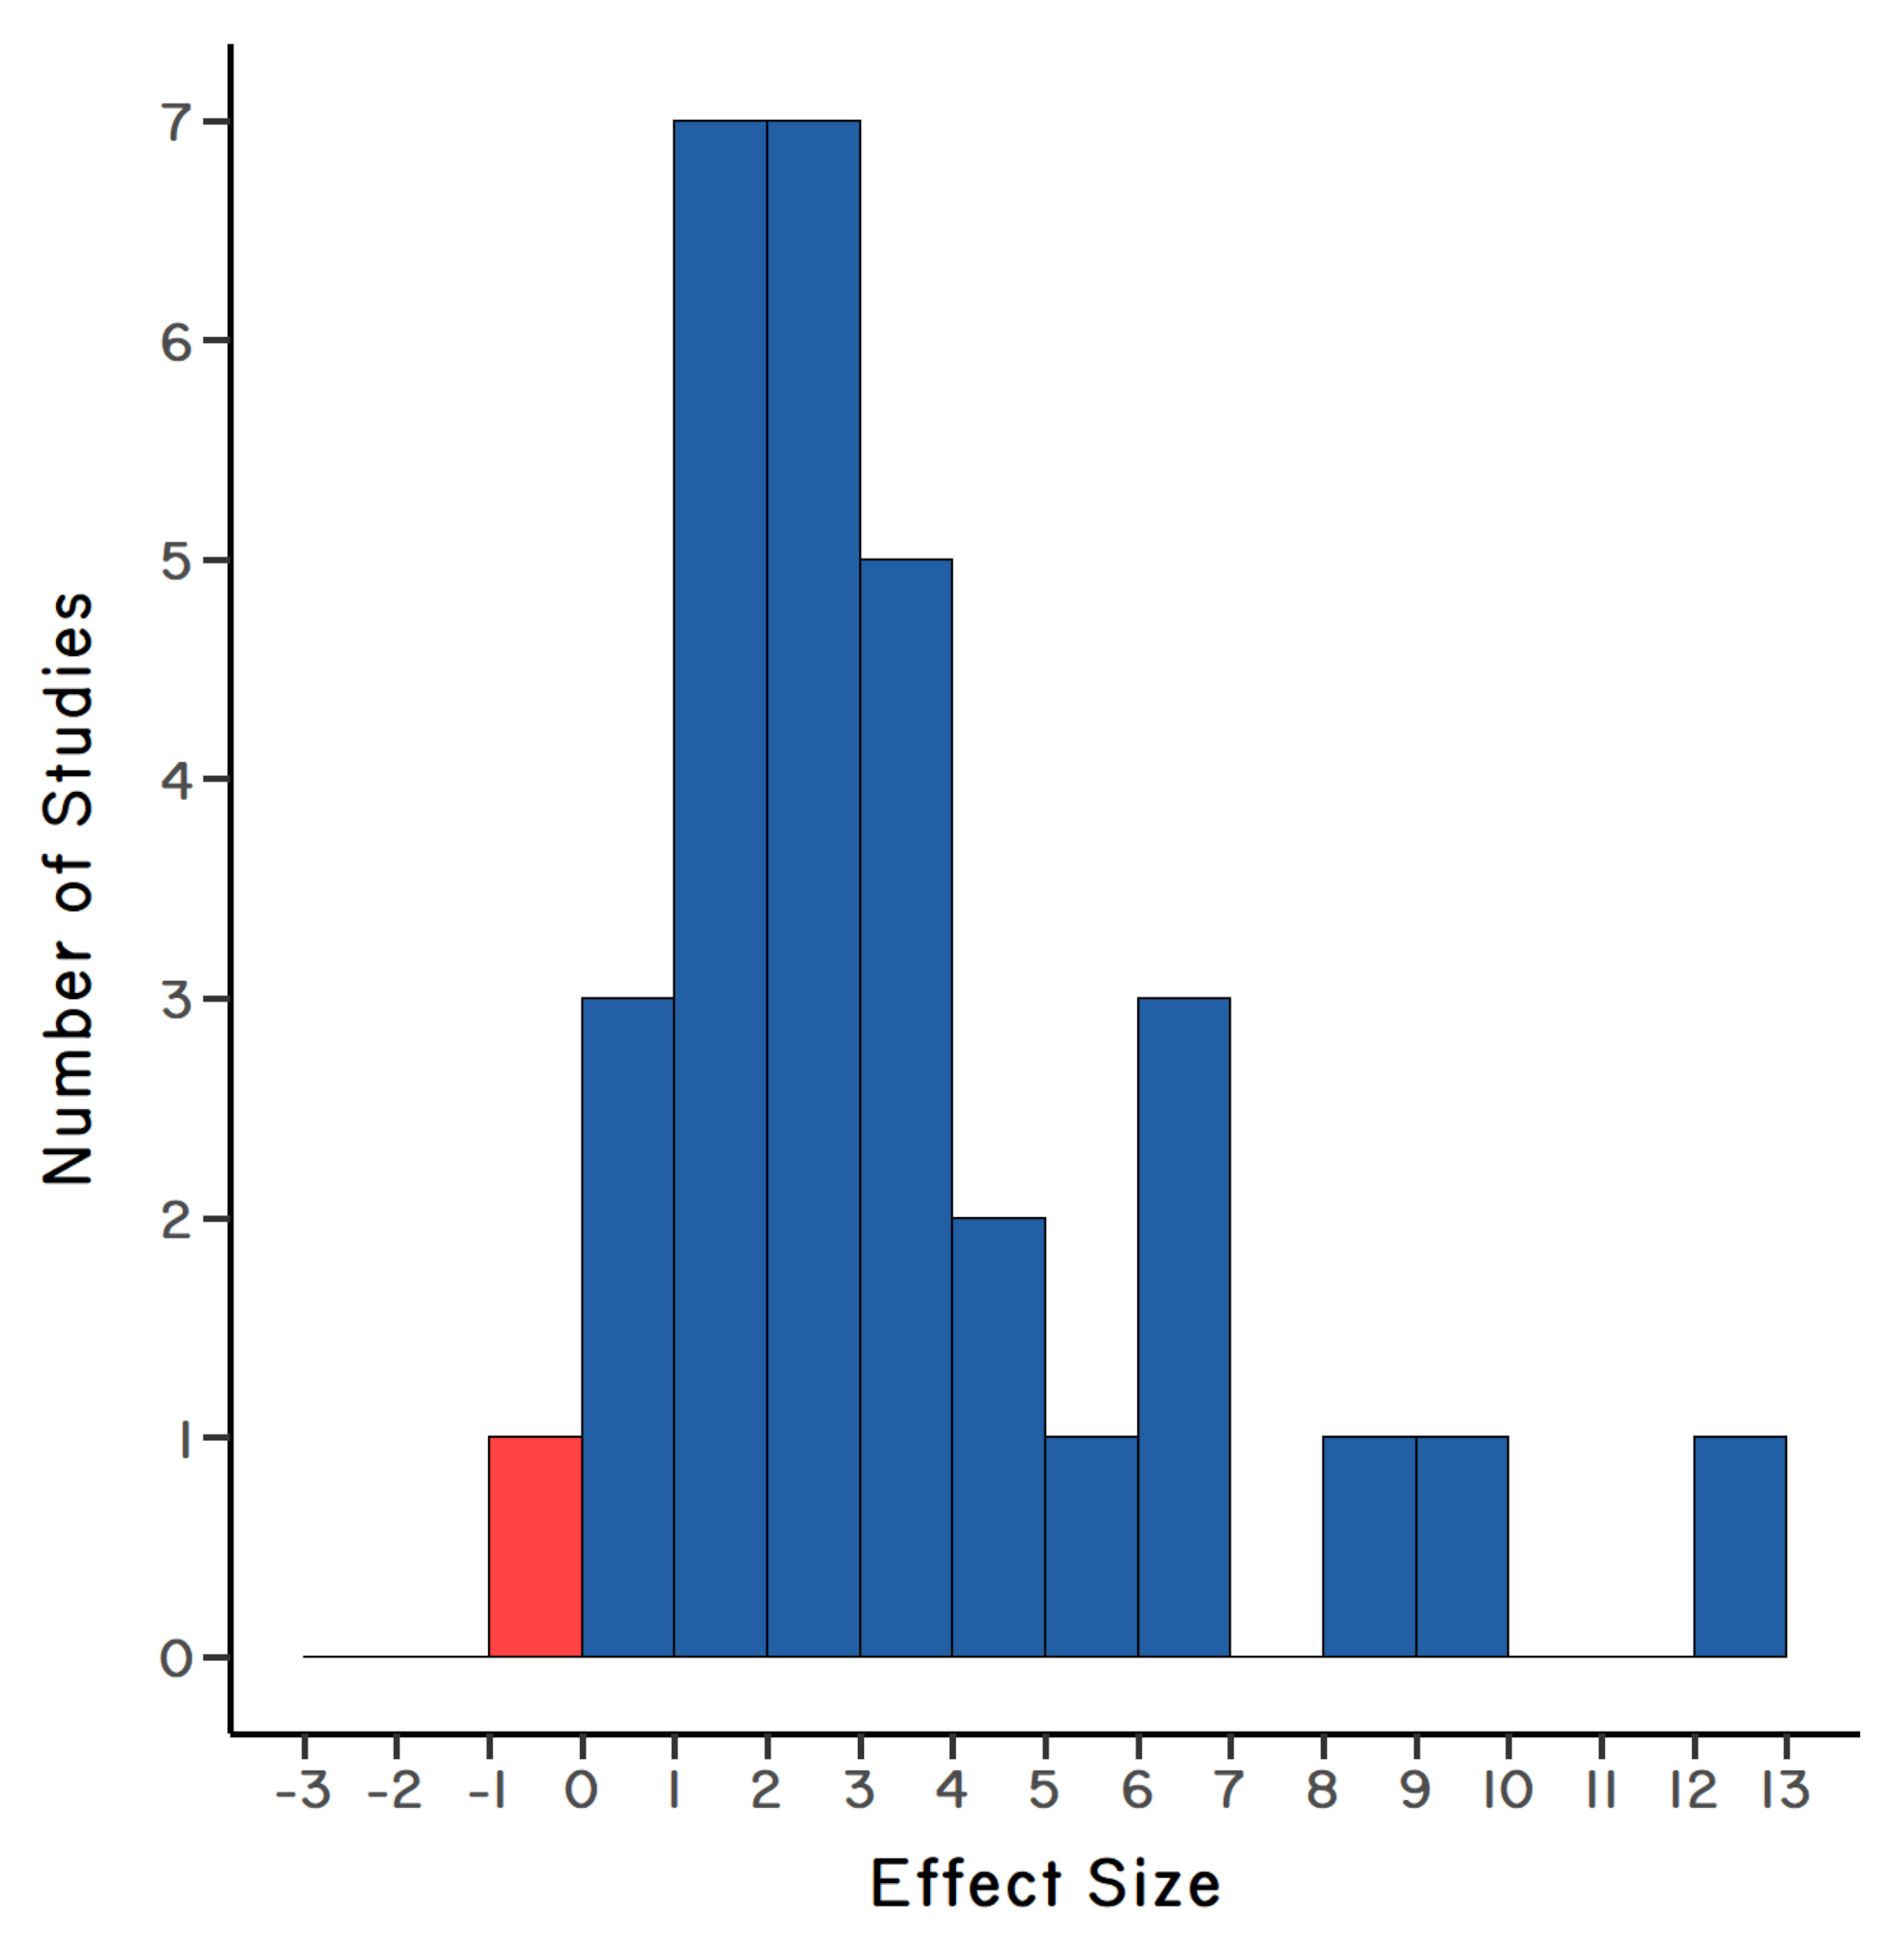
\includegraphics[width=0.6\textwidth,height=\textheight]{images/fig4-6.png}

}

\caption[Results from a meta-analysis of local adaption
experiments]{\label{fig-4.5}Results from a meta-analysis of local
adaption experiments. The ``effect size'' depends on the magnitude of
the difference between the proportion of infection in sympatric versus
allopatric hosts, where positive values indicate that the parasite is
adapted to infecting snails from the local host population. Large effect
sizes are indicative of stronger local adaptation by parasites. Positive
effect sizes are shown in blue; negative effect sizes are shown in red.
A statistical test on the effect sizes showed that, in general, the
parasite is strongly adapted to infecting local populations of its host.
There were 32 total sympatric/allopatric comparisons. (Redrawn from
\citeproc{ref-lively2004a}{Lively \emph{et al.} 2004}).}

\end{figure}%

\section{Self- / Non-Self-Recognition}\label{self--non-self-recognition}

In my presentation thus far, I have been assuming that the molecules on
the cell surfaces of parasites must mimic host molecules to evade
detection. Otherwise, the parasites will be identified as foreign and
killed by the host. In other words, there is a self- /
non-self-recognition system in hosts, which is determined by a
polymorphic set of alleles at one or more loci.

Where did this idea for self- / non-self-recognition come from? I am
embarrassed to say that I did not know before writing this chapter, and
I am still not exactly sure, but the idea goes back at least to Sir
Frank McFarland Burnet, who was cowinner of the 1960 Nobel Prize in
Physiology and Medicine (with Sir Peter Medawar). Burnet was reviewing
two studies, which showed recognition and rejection of genetically
different competitors of the same species
(\citeproc{ref-burnet1971a}{Burnet 1971}). The first study was from
Hidemiti Oka (\citeproc{ref-oka1970a}{1970}): ``Here I shall explore the
possibility that Oka's (\citeproc{ref-oka1970a}{1970}) studies of
colonial tunicates (\emph{Botryllus}) \ldots{} may throw light on
primitive types of `self and not-self' recognition from which adaptive
immunity may have evolved.'' Hidemiti Oka was a Japanese professor of
biology in Tokyo. He was following up on a pioneering study by Bancroft
(\citeproc{ref-bancroft1903a}{1903}), who had shown that fragments from
related colonies of a compound ascidian (\emph{Botryllus schlosseri})
readily fused, whereas fragments from unrelated colonies rejected each
other. Oka's goal was to understand the genetic basis for this
fusion/rejection. His study suggested that fusion was determined by
multiple alleles (``perhaps several scores'') at a single locus. More
specifically, Oka's results suggested that fusion occurred between
different colonies only if they shared at least one allele at this
locus.\footnote{In direct contrast, however, Oka found that
  cross-fertilization did not occur between \emph{Botryllus} gametes
  that shared the same allele. As Oka noted, this result mirrors the
  S-allele system in plants: ``The \ldots{} situation corresponds
  exactly in its form to the homomorphic self-incompatibility prevailing
  among angiosperms.''} To my mind, this was a major finding.

It thus appears that Oka was inspired by Bancroft, and Burnet was
inspired by Oka. How does Burnet fit in? Burnet first accepts Oka's
assumption that allorecognition depends on a single highly polymorphic
locus (Figure~\ref{fig-4.6}): ``To summarize Oka's work, it is
convenient to accept his assumption, which is validated by much
preliminary work, that fusion or rejection between colonies depends on a
single locus with many alleles which can be referred to as recognition
genes.'' Burnet then suggests that this same mechanism could be co-opted
as a defense against parasites and that such a mechanism could be the
progenitor of the more sophisticated adaptive immune system in
vertebrates. Burnet (\citeproc{ref-burnet1971a}{1971}) writes:

\begin{quote}
It is probably unwise to attempt to imagine the various steps by which
such changes could be made. One can foresee a period of great research
activity in these fields of tissue fusion and rejection in invertebrates
and protochordates during the next decade. Undoubtedly a variety of
intriguing phenomena will be uncovered, differing from group to group.
Some may be further along the road toward adaptive immunity than the
colonial ascidians. Much more extensive comparative studies are called
for and in due course analysis of the results should allow a clear
evolutionary history to emerge. Whatever form that history eventually
takes we can be certain that gene duplication (gene expansion) plays a
major part, and that progressive specialization of cell function and
phenotypic restriction will be as conspicuous as it is in all other
organs and functions. \textbf{Copyright © 1971, \emph{Springer Nature
Limited}}
\end{quote}

Wow. In retrospect, Burnet's ``attempt to imagine the various steps''
does not seem at all unwise. In any case, he suggests that infection
occurs when parasites have alleles that match their host's genotype.
Otherwise, the parasites are killed. This is the logic of what will
later be called the ``matching alleles model'' for infection.

\begin{figure}

\centering{

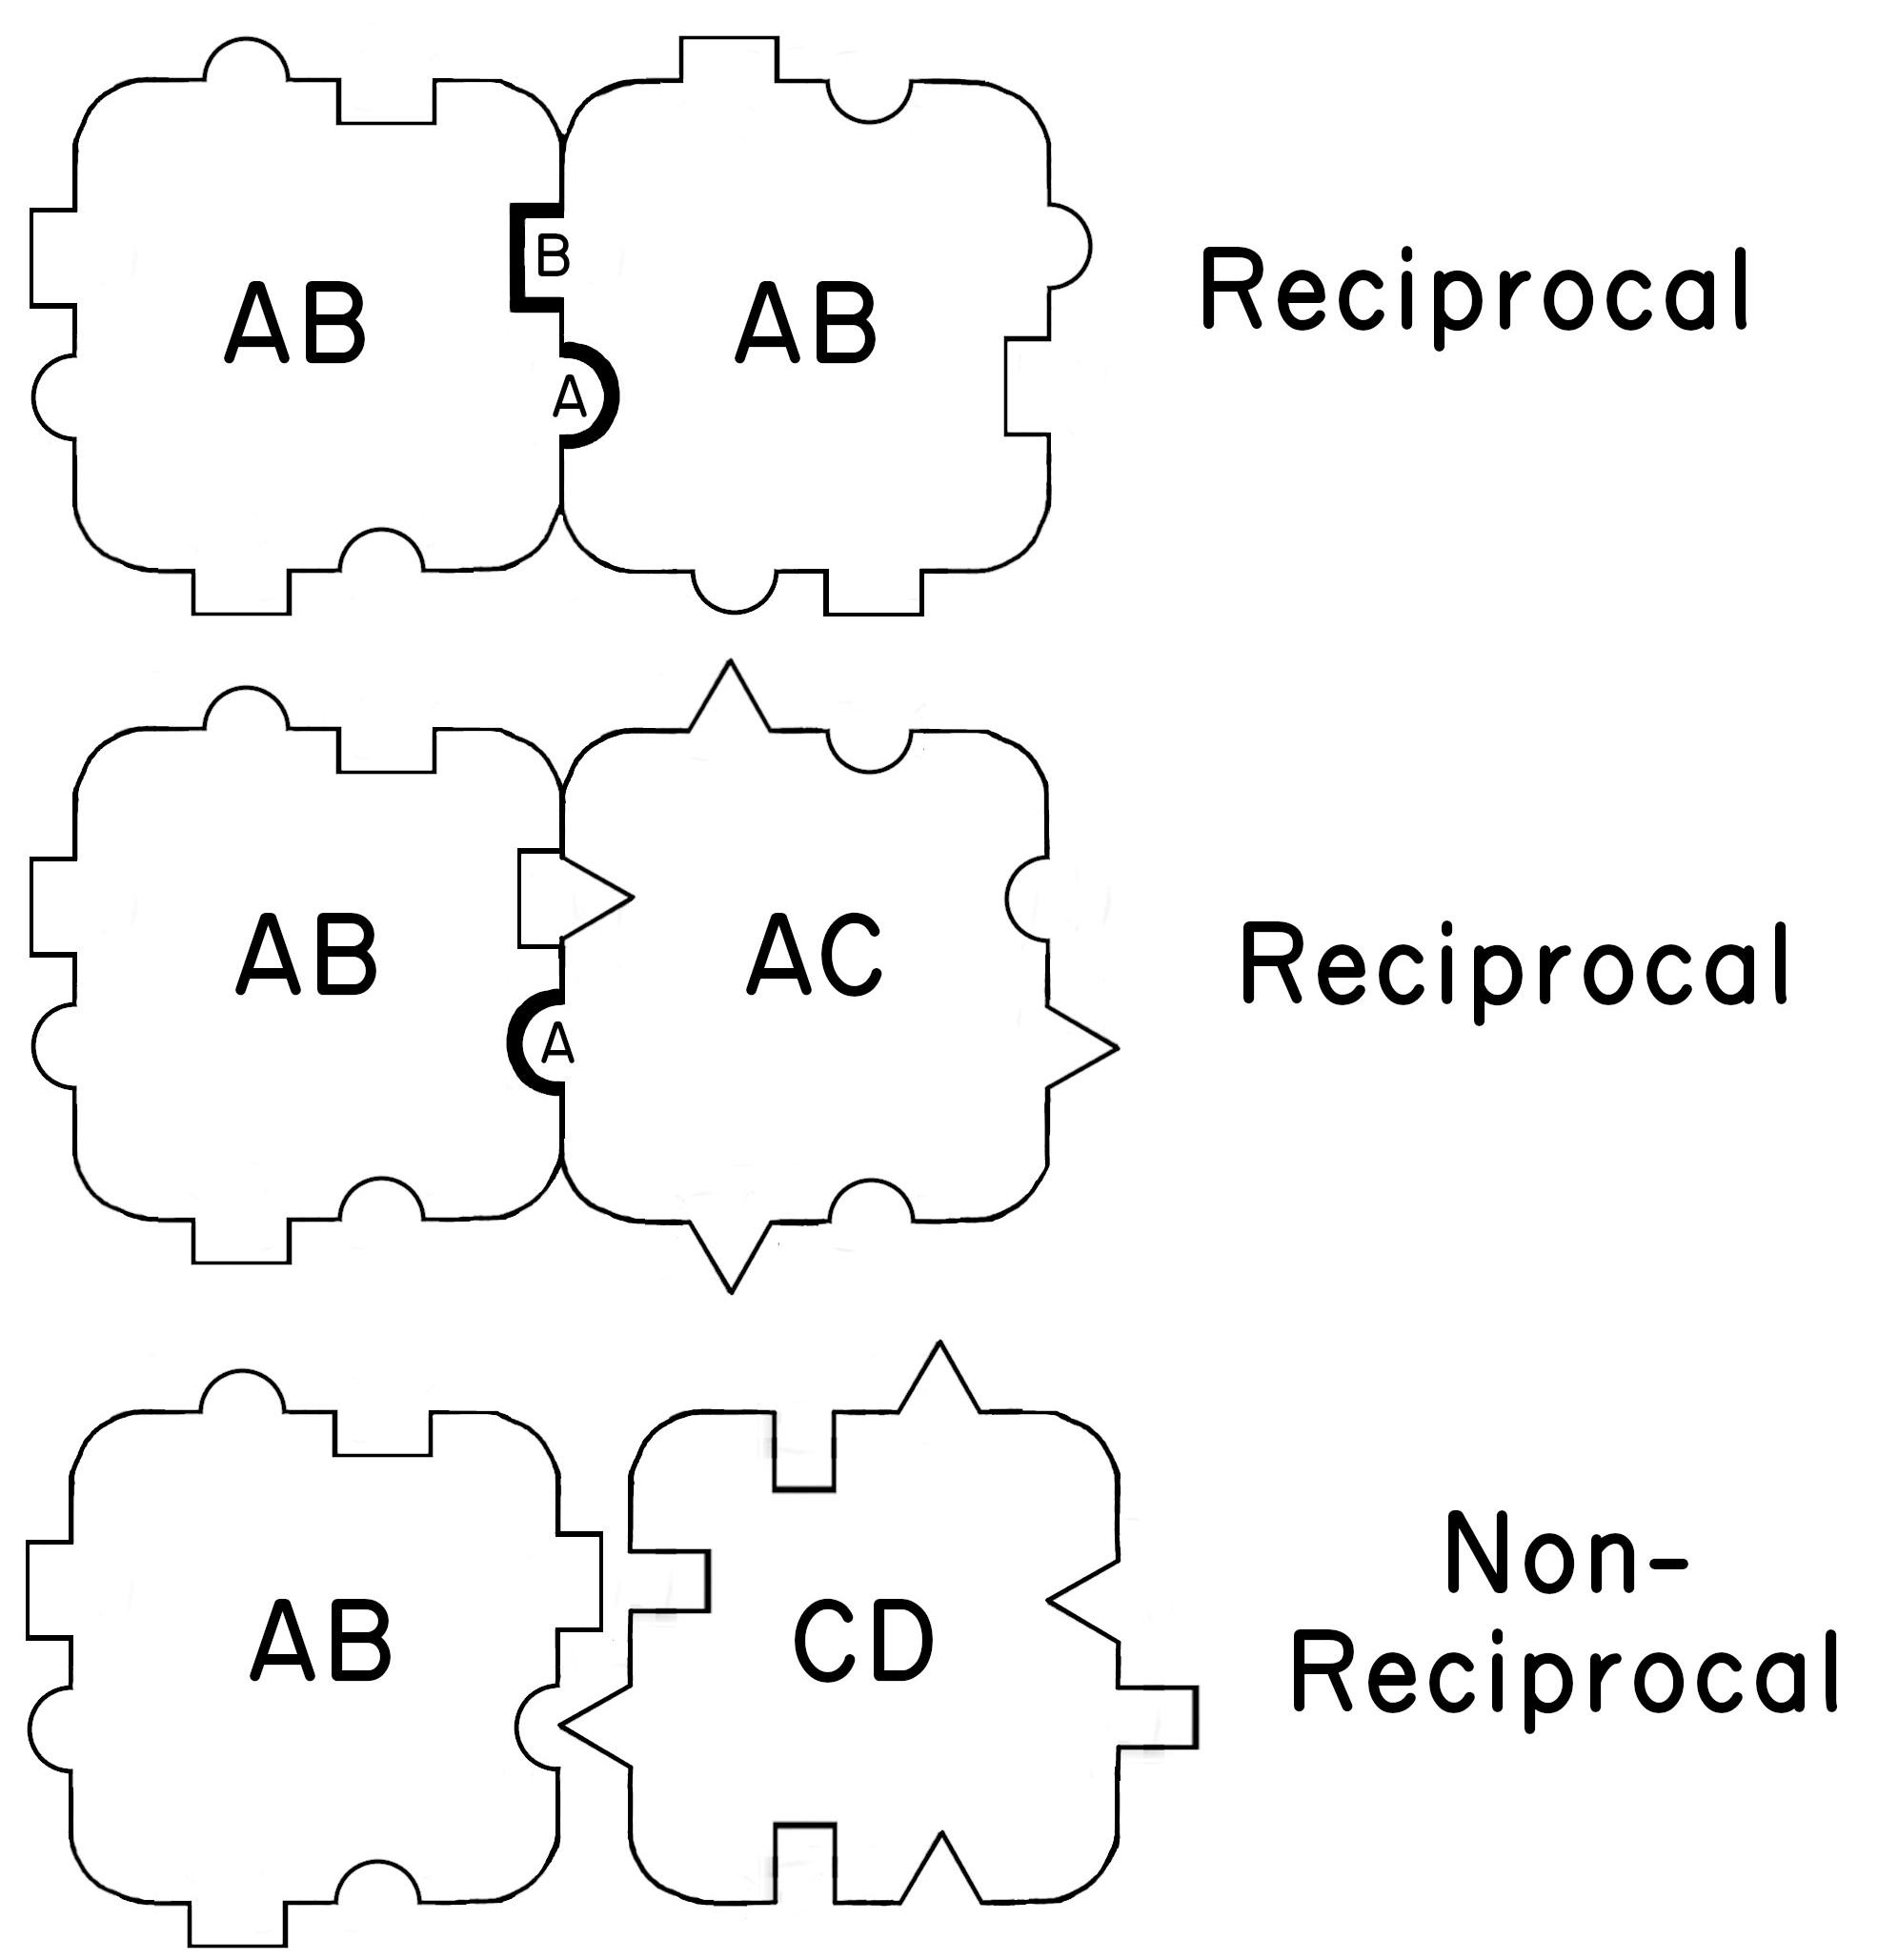
\includegraphics[width=0.55\textwidth,height=\textheight]{images/fig4-7.jpeg}

}

\caption[A model for self- / non-self-recognition]{\label{fig-4.6}A
model for self- / non-self-recognition
(\citeproc{ref-burnet1971a}{Burnet 1971}; \citeproc{ref-oka1970a}{Oka
1970}). Cells sharing one or more alleles can rejoin after separation,
as the receptors match. In contrast, cells that do not share an allele
do not match and will not rejoin. Regions of fusion are shown in heavy
lines. Burnett suggested that resistance in host-parasite interactions
could have a similar mechanistic framework. Note that Burnett used
``reciprocal'' for matching cells with at least one matching allele, and
``non-reciprocal'' for cells in which none of the alleles matched.
Redrawn from Burnet (\citeproc{ref-burnet1971a}{1971}) by Zoe M Dinges.}

\end{figure}%

\section{Summary}\label{summary-3}

\begin{enumerate}
\def\labelenumi{\arabic{enumi}.}
\tightlist
\item
  The most common trematode infection in lake populations of \emph{P.
  antipodarum} is caused by a larval stage of \emph{Microphallus} sp.
  (recently renamed to \emph{Atriophallophorus winterbourni}). The
  trematode has a two-host life cycle (snails and waterfowl).
\item
  Experimental cross-inoculation experiments showed that
  \emph{Microphallus} is more infectious to local lake populations of
  its snail host, \emph{P. antipodarum}, than to remote host
  populations.
\item
  These results suggest that some kind of match by the parasite to the
  host is required for infection. This idea of matching is consistent
  with the idea of self- / non-self-recognition as the basis for immune
  defense. The gist of the original idea stems from experimental studies
  of colony fusion in tunicates.
\end{enumerate}

\bookmarksetup{startatroot}

\chapter{Gynogenetic Fish}\label{sec-gyno}

\begin{center}
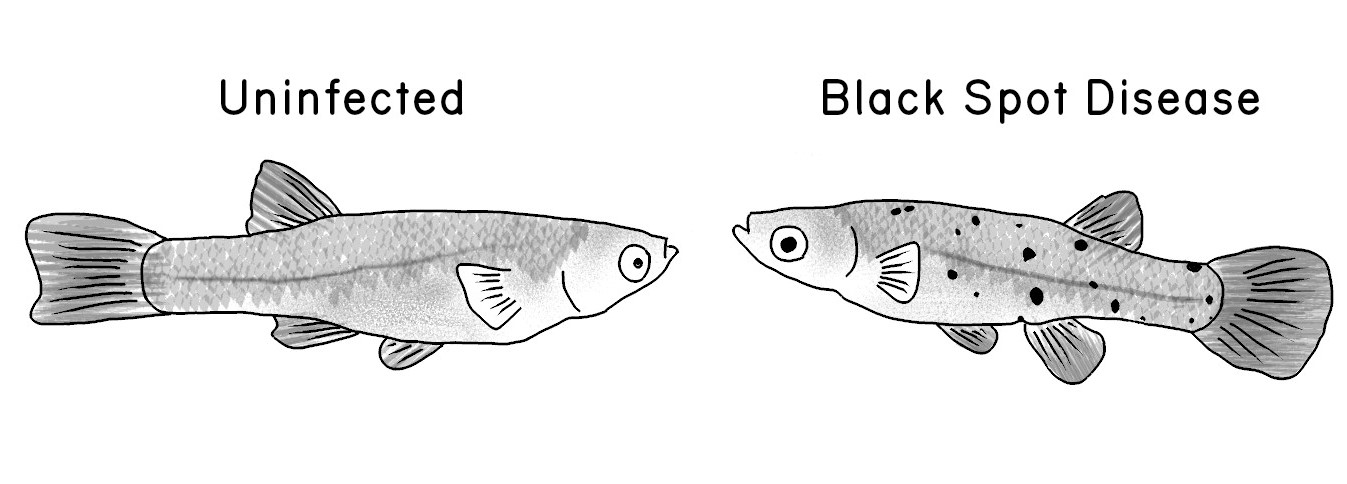
\includegraphics{images/fig5-1.jpeg}
\end{center}

New Zealand felt like home after five years, and we had many good
friends and colleagues in Christchurch, especially David Lloyd. David
and I talked often about strategic models of natural selection (game
theory), of which he was one of the world's leaders. I was particularly
influenced by his idea that sexual reproduction, polymorphism,
phenotypic plasticity, and hermaphroditism could all be seen under the
umbrella of ``variation strategies'' (\citeproc{ref-lloyd1984a}{Lloyd
1984}). Sadly, when Lynda completed her PhD, her visa expired, and we
had to leave New Zealand. But where to go?

Lynda was a rising star when she completed her PhD. She landed a
post-doc at Rutgers University to work with Tom Meagher, so we moved to
New Jersey in January 1989. Once again, Lynda was supporting us. Steven
Handel gave me a desk and some space in his lab. Soon afterward, Peter
Morin asked me to give a seminar on sex/asex at Rutgers. I knew of
Peter's pioneering work in community ecology for which he had received a
young investigator's award from the Ecological Society of America (the
Mercer Award). I was quite nervous to give a seminar in front of one of
my heroes. Another of my heroes, Professor Bob Vrijenhoek, was also in
the audience. As described in Section~\ref{sec-niche}, Bob was the
creative mind behind the Frozen Niche-Variation Hypothesis, and he was
well known for his work on sexual and asexual fish (topminnows in the
genus \emph{Poeciliopsis}). He was also the director of the Center for
Theoretical and Applied Genetics (CTAG) at the New Brunswick campus of
Rutgers University, and he was the Editor-in-Chief of the journal
\emph{Evolution}, the most prestigious journal in evolutionary biology.
After my talk, Bob, Peter, Lynda, and I went out for dinner. Somewhere
in the middle of the meal, Bob offered me a post-doc to work with him at
CTAG. I was dumbfounded. But I managed to say yes, ``When do I start?''
He said, ``How about tomorrow?''

For this to make sense, you need to know more about Vrijenhoek's fish.
Like the snails, the fish have coexisting sexual (diploid) and asexual
(triploid) forms. The asexual fish, however, were ``gynogenetic,'' which
means that the eggs require fertilization to kick-start embryogenesis.
The sneaky eggs, however, do not generally incorporate the sperm's DNA
(review in \citeproc{ref-vrijenhoek1998a}{Vrijenhoek 1998}).\footnote{Paternal
  leakage of DNA in otherwise asexual vertebrate species now seems
  possible (review in \citeproc{ref-lampert2010a}{Lampert \& Schartl
  2010}).} The outcome is the coexistence of sexual and asexual lineages
within the same semi-isolated populations.

Bob had worked on these fish for decades, focusing on small streams in
Mexico. He had worked in particular on the coexistence of a sexual form
of the fish, \emph{Poeciliopsis monacha}, with two gynogenetic clones,
which were interspecific hybrids between \emph{P. monacha} and \emph{P.
lucida} (\citeproc{ref-vrijenhoek1978a}{Vrijenhoek 1978},
\citeproc{ref-vrijenhoek1979a}{1979}). The triploid clones were
independently derived from their sexual ancestors, with two copies of
the monacha genome and one copy of the lucida genome
(\citeproc{ref-schultz1969a}{Schultz 1969}). During his studies, Bob had
frozen fish for many years from several of his sites. He remembered that
some of the fish in his freezer were heavily infected with black-spot
disease. The black spots are clearly visible on the body of the fish.
The spot itself is caused by trematode larvae that burrow into the fish
and encyst (genus \emph{Uvulifer}). The fish's immune system then coats
the cyst with melanin, which turns the cysts black. Bob thought it would
be interesting to see if the asexual fish were more infected than the
sexuals. The prediction under the Red Queen Hypothesis was that the most
common asexual clones would be most infected by black spot disease
(Section~\ref{sec-app-5}).

Bob enlisted the help of one of his PhD students, Clark Craddock. Clark
ran the allozyme electrophoresis, which was necessary at the time to
tell sexual fish from the two clones. She also helped count the cysts,
run the statistics, and write the paper. We found right away that larger
fish had more cysts, which makes sense. But we also found that the most
common clone, clone 1, had significantly more black spots per unit body
length than the sexual fish in Log Pool (Figure~\ref{fig-5-1} A \& B).
In addition, the sexual fish showed greater size-corrected variation in
the number of parasitic cysts than the asexual fish, which makes sense
if the sexual population contained genetic variation for resistance to
infection. So, after correcting for size, the sexual fish were both less
infected and showed more variation in infection than the clone
2.\footnote{In a follow-up study (using different samples), Weeks
  (\citeproc{ref-weeks1996a}{1996}) did not find some of our significant
  effects. His sample sizes, however, were small, suggesting that his
  power to detect differences was low.} This seemed very promising for
the Red Queen.

Similar results were observed in a second pool (Sandal Pool) in which
both clones coexisted. In this pool, clone 2 was more common than clone
1, and it was also more infected than clone 1 (Figure~\ref{fig-5-2}).
However, clone 1 was not more infected than the sexual form of P.
monacha, which showed that clone 1 is not inherently more susceptible to
infection (\citeproc{ref-lively1990a}{Lively \emph{et al.} 1990}). Taken
together, the results suggest that the parasites had evolved to
disproportionately attack the most common local clone.

\begin{figure}

\centering{

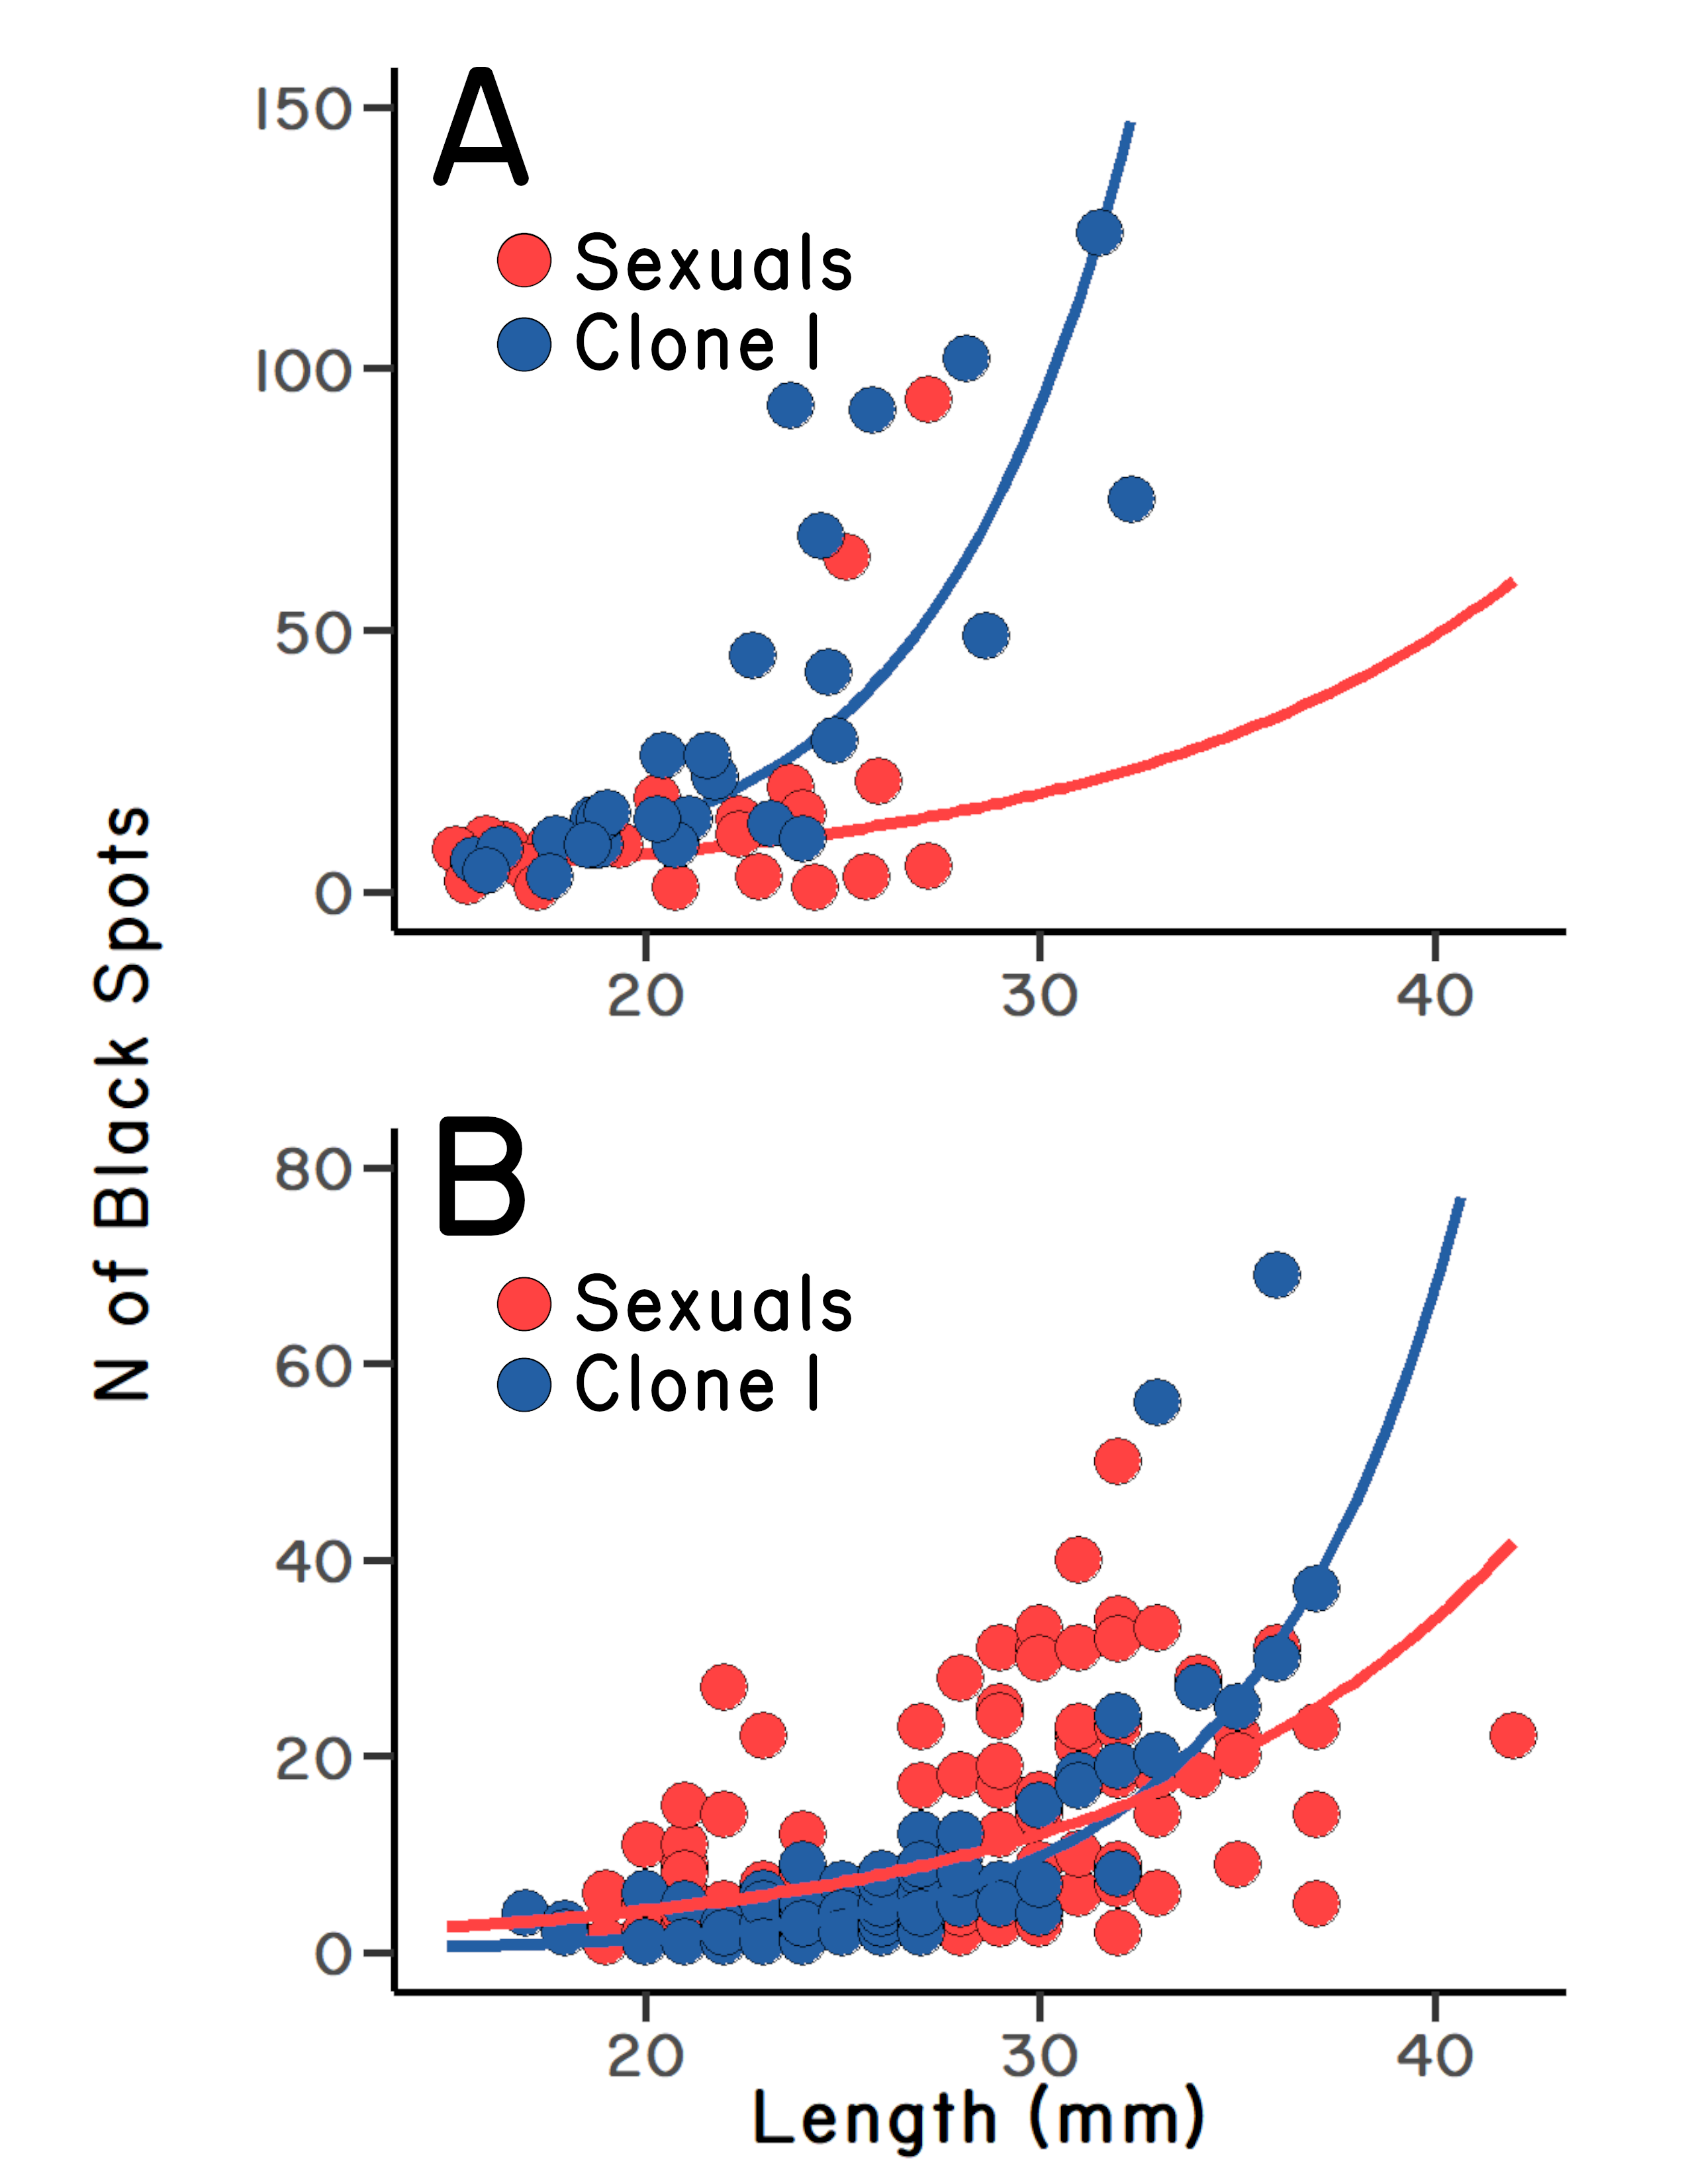
\includegraphics[width=0.6\textwidth,height=\textheight]{images/fig5-2.png}

}

\caption[Number of trematode larvae per fish in Log
Pool]{\label{fig-5-1}Number of trematode larvae per fish in Log Pool.
\textbf{A.} Log Pool 1978 (number of sexuals = 23, number of clone 1 =
29). \textbf{B.} Log Pool 1985 (number of sexuals = 91, number of clone
1 = 81). In both years, the sexual fish showed greater residual
variation in infection than clone 1, which hints at an underlying
genetic basis for infection. Redrawn from Lively et al.
(\citeproc{ref-lively1990a}{1990}). Note that y axes are the number of
trematode larvae plus one.}

\end{figure}%

\begin{figure}

\centering{

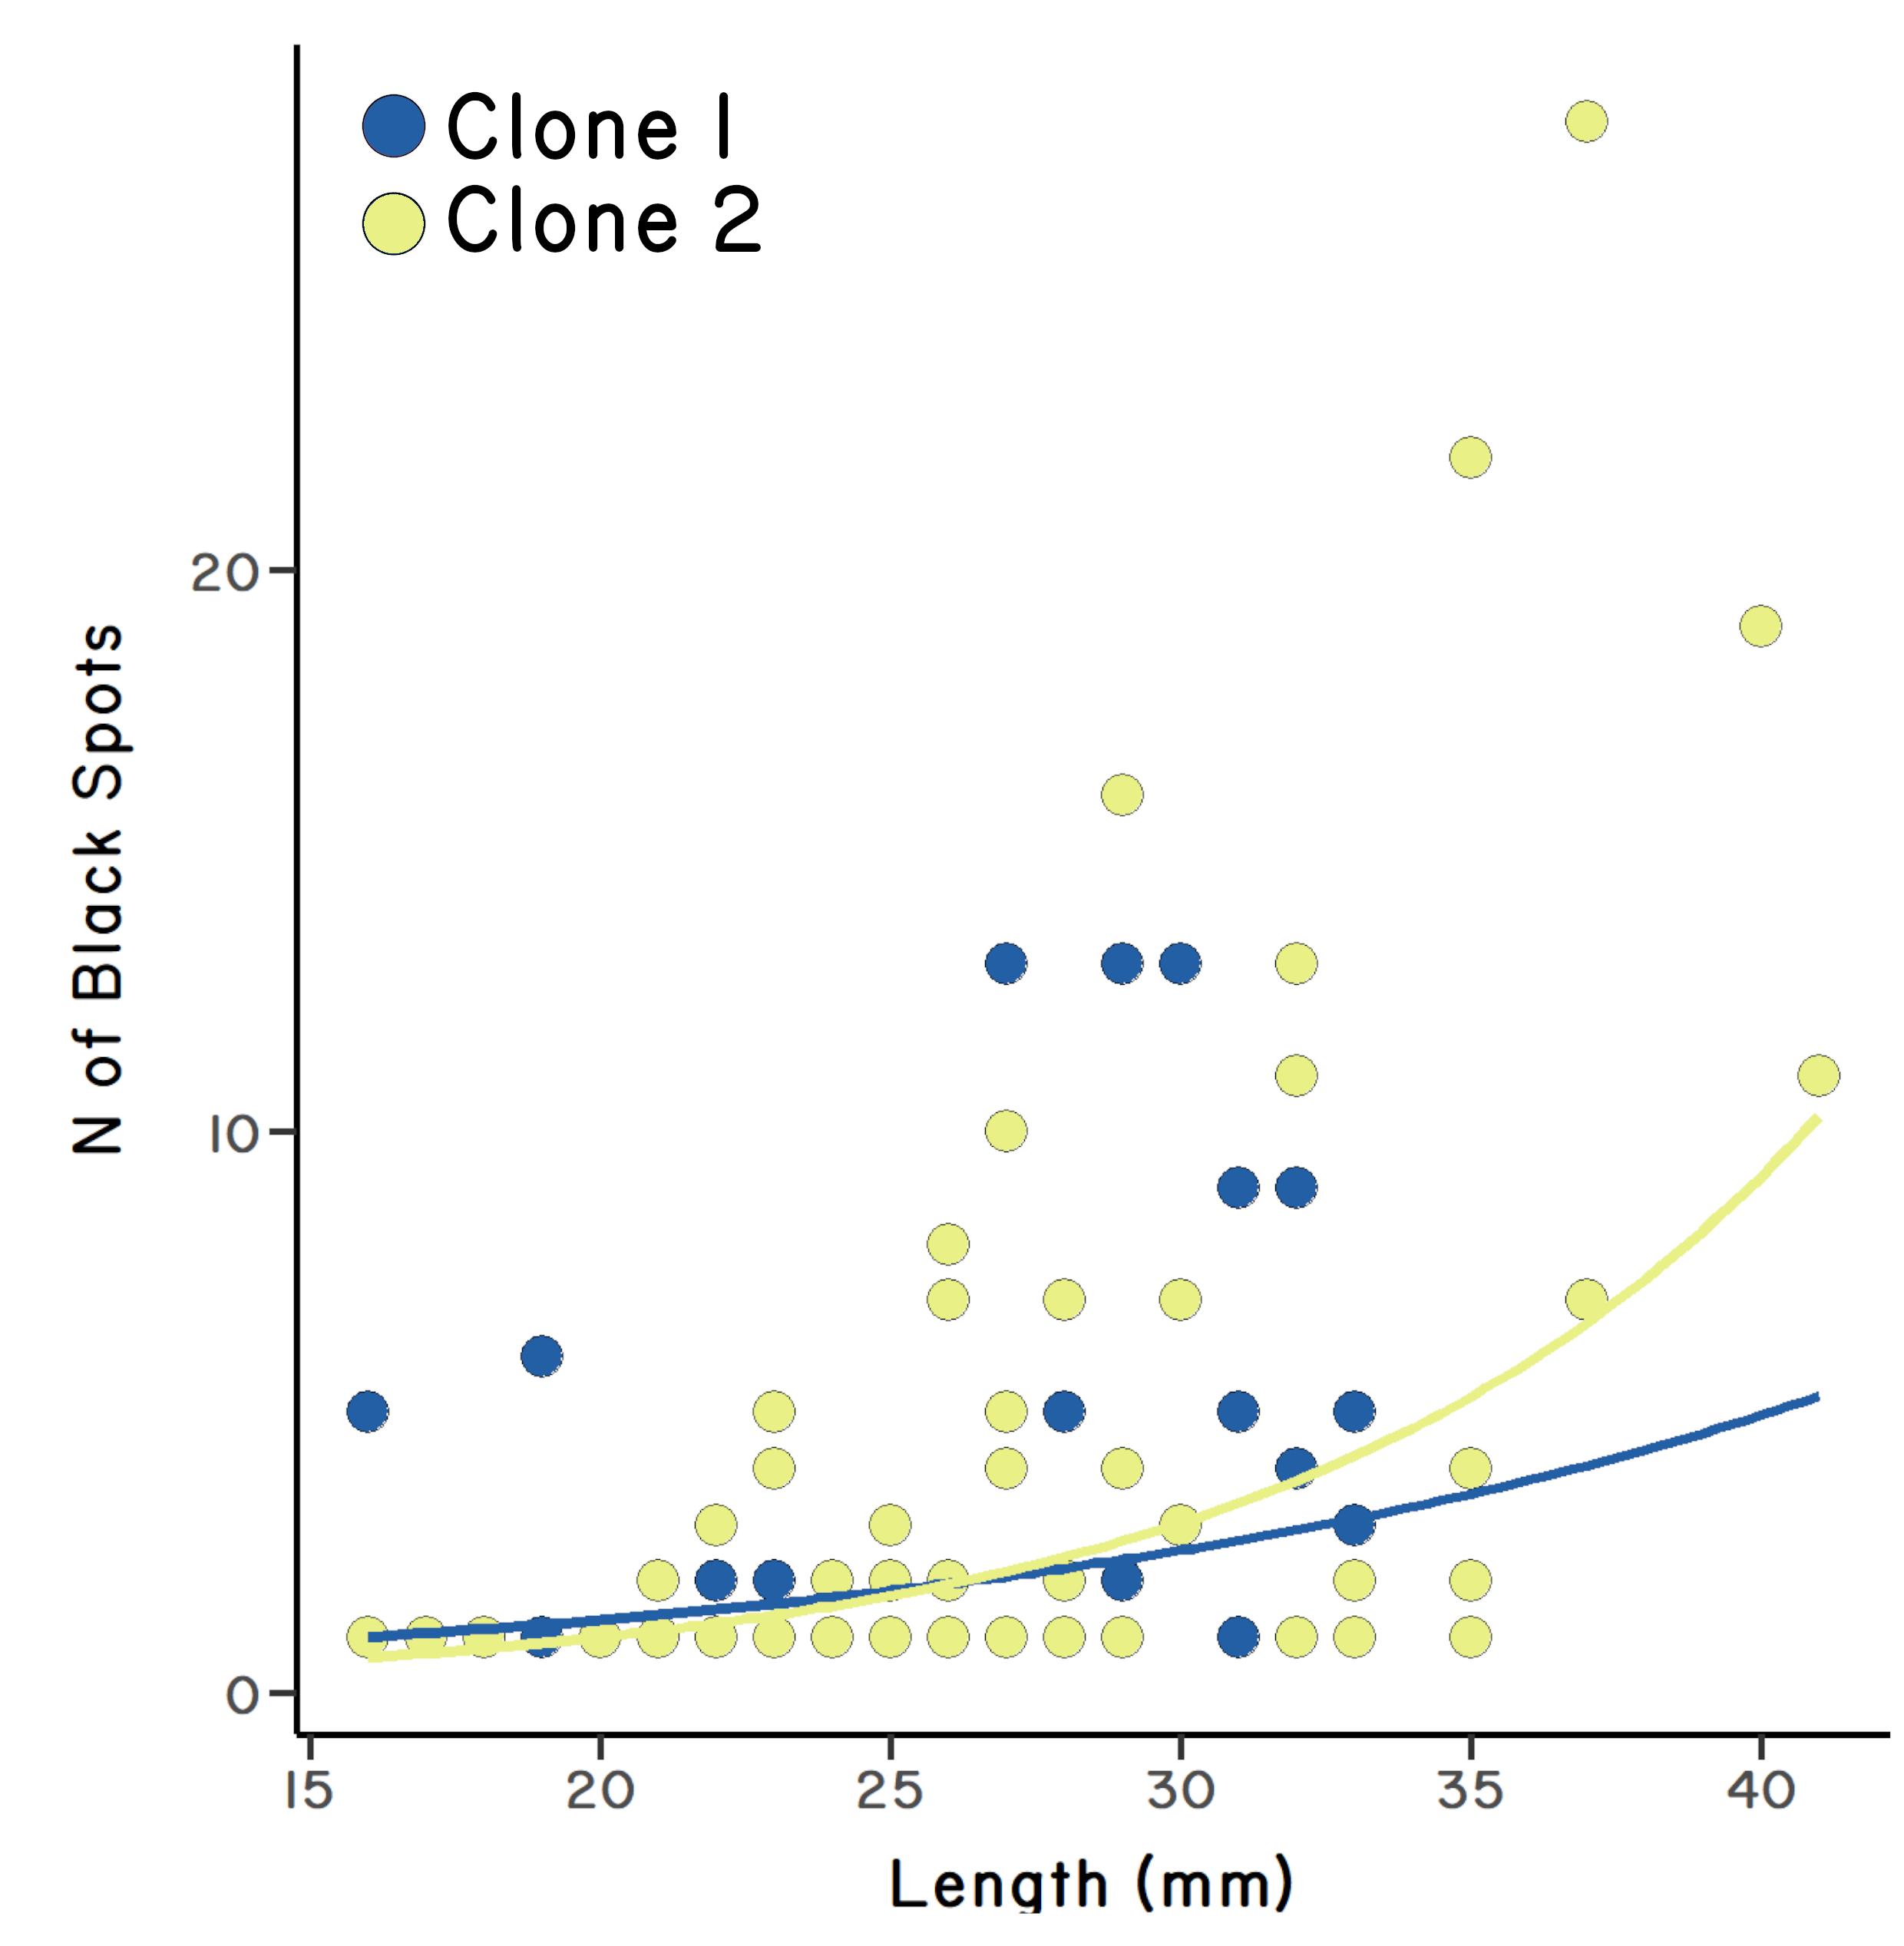
\includegraphics[width=0.6\textwidth,height=\textheight]{images/fig5-3.png}

}

\caption[Number of trematode larvae infecting clones 1 and 2 in Sandal
Pool 1985]{\label{fig-5-2}Number of trematode larvae infecting clones 1
(\(N=44\)) and 2 (\(N=75\)) in Sandal Pool 1985. The curve for the
sexual population (\(N=138\), not shown) is very similar to the curve
for clone 1. Redrawn from Lively et al.
(\citeproc{ref-lively1990a}{1990}).}

\end{figure}%

But we had more samples to run. When we examined another pool, the trend
reversed: sexual fish were more infected than asexual fish
(Figure~\ref{fig-5-3} A). We were confused. I remember Clark telling Bob
of this new result. He said something like, ``Well, that's science,''
and then headed back to his office. He was halfway there when he turned
around and asked, ``what sample was that?'' Clark told him, ``Heart
Pool, 1983.'' Bob got a big smile. Then he told us that, in that sample,
the sexual fish were highly inbred. The population had descended from a
small number of founders, and they were homozygous for most loci. So,
the sexual fish were more infected in that sample, but they were also
genetically depauperate. Under the Red Queen, there is no value to
sexual reproduction unless there is genetic variation in the population.
On the other hand, the greater level of infection in sexual fish might
have been caused by inbreeding depression, which was known for other
fitness-related traits (\citeproc{ref-vrijenhoek1982a}{Vrijenhoek \&
Lerman 1982}).

It was an amazing set of results, but there was another twist. Bob had
added some fish (in 1983) to the isolated founder population in Heart
Pool. His goal was to increase the genetic diversity of the sexual
population. After a few years, he resampled the site, and fortunately,
he had saved the samples in his freezer from 1985. Clark and I had a
look. The pattern had reversed: now the sexual fish were less infected
than the asexual fish (Figure~\ref{fig-5-3} B). In addition, the
size-corrected variance in infection had increased in the sexual fish in
just two years. The advantage to outcrossing seemed to depend on genetic
diversity.

In summary, the data suggested that the parasites had evolved to infect
the most common local host clone in the different pools. They also
suggested that sex in genetically diverse host populations results in
protection from disease. Both results were consistent with the Red
Queen.\footnote{It is important to point out that we were not claiming
  that parasite-mediated selection is maintaining sex in this system.
  For example, we wrote, ``{[}W{]}e do not intend to imply from this
  analysis that the trematode is selecting for the maintenance of sex in
  these fish.'' Niche partitioning and/or the sperm-dependence of the
  gynogenetic females would most likely ensure the persistence of sexual
  individuals (\citeproc{ref-moore1971a}{Moore \& McKay 1971};
  \citeproc{ref-Schenck1986a}{Schenck \& Vrijenhoek 1986}). Our claim
  was simply that parasites had evolved to disproportionately infect the
  most common clone unless the sexual population was highly inbred.}
Proof? No.~Fascinating? Yes. In any case, looking back, I was very lucky
to have had the opportunity to work with Professor Vrijenhoek.

\begin{figure}

\centering{

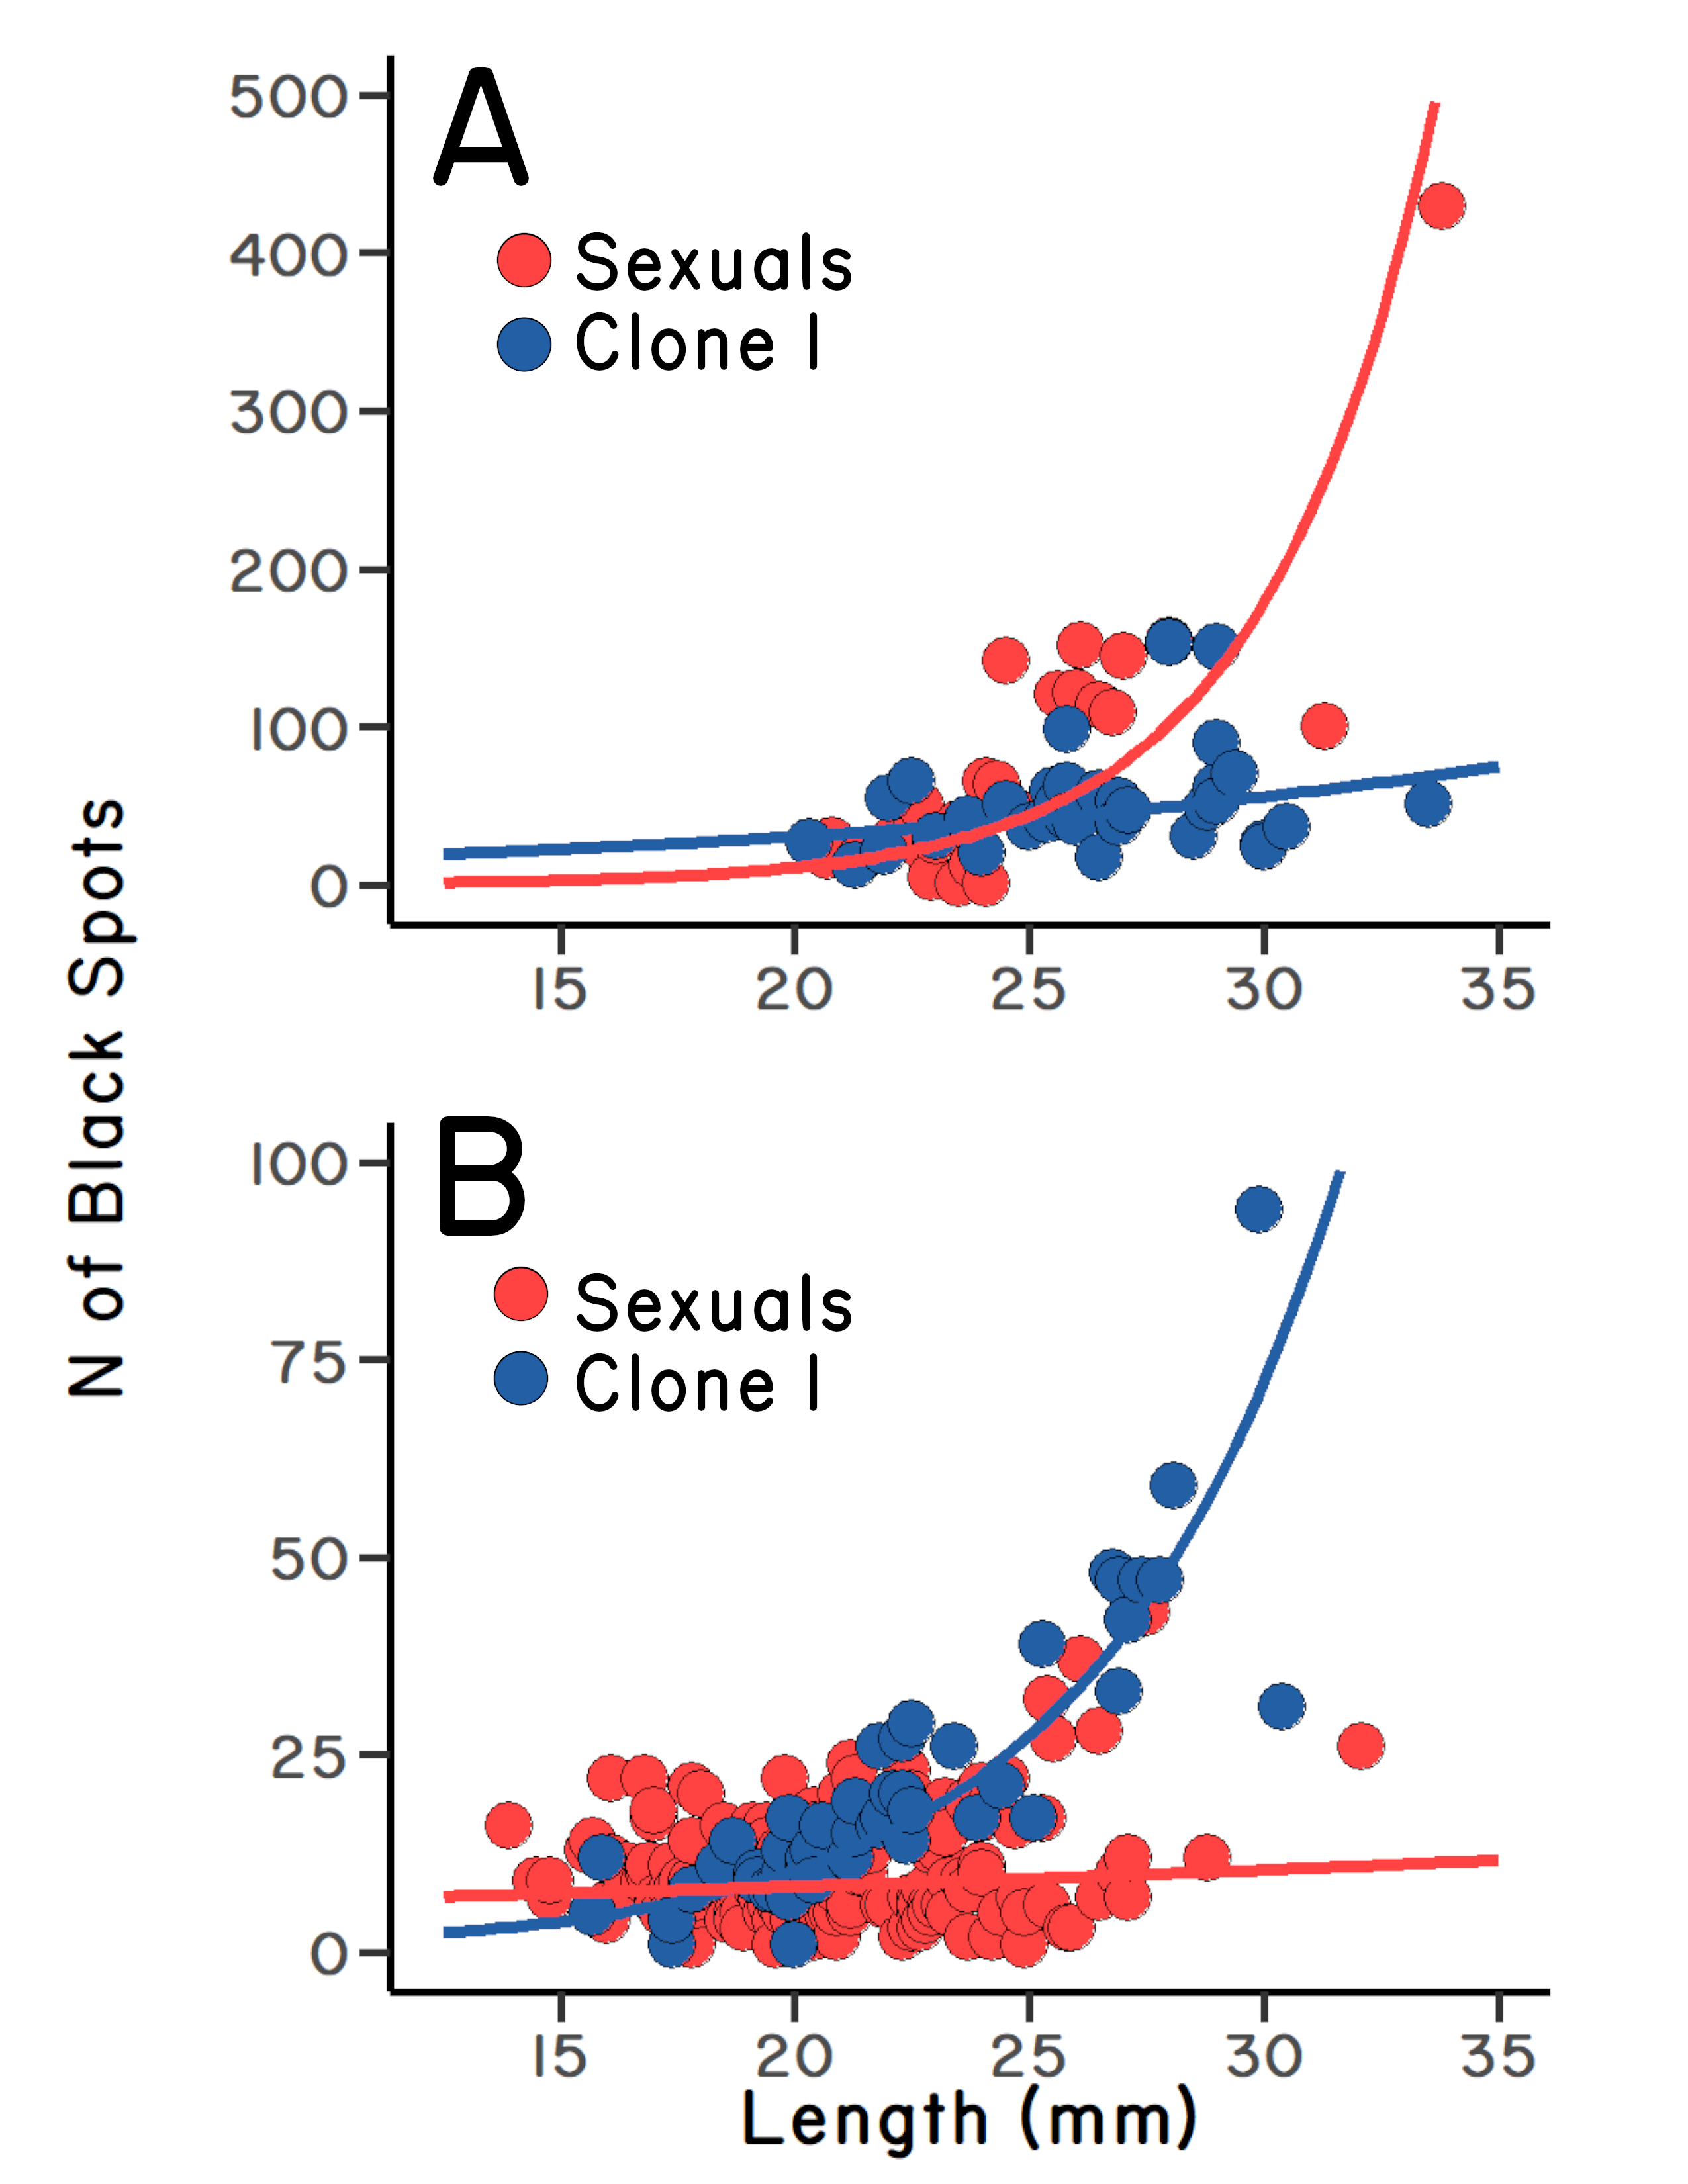
\includegraphics[width=0.6\textwidth,height=\textheight]{images/fig5-4.png}

}

\caption[Number of trematode larvae infecting fish in Heart
Pool]{\label{fig-5-3}Number of trematode larvae infecting fish in Heart
Pool. \textbf{A (top):} Heart Pool 1983 (number of sexuals = 27; number
of clone 1 = 34). The sexual fish in the pool were highly inbred and
they were also significantly more infected per unit length than clone 1.
The result remained significant after removing the apparent outlier in
the sexual population with more than 400 cysts (black spots). The
residual variances in the number of cysts were not significantly
different between the inbred sexual fish and clone 1. \textbf{B
(bottom):} Heart Pool 1985 after the infusion of genetic variation into
the pool. Here the sexual fish (\(N=171\)) were less infected than the
coexisting clone (\(N=48\)), and they showed significantly greater
residual variation for infection than the clone, similar to the results
for Log Pool. Redrawn from Lively et al.
(\citeproc{ref-lively1990a}{1990}).}

\end{figure}%

\section{Appendix: Within Versus Between Populations}\label{sec-app-5}

It can be a bit confusing, but I think that the predictions of the Red
Queen Hypothesis depend on whether one is looking \textbf{within versus
between populations}. In Chapter~\ref{sec-eco-hyp-cont}, I suggested
that snail populations having more parasites should be more likely to
have some sexual reproduction. Here I am suggesting that asexual fish
would be expected to have more parasites. How does that work?

\textbf{Between populations} we would expect to find that host
populations without coevolving parasites would evolve to reproduce by
parthenogenesis. As such, sex should be positively correlated with
infection prevalence. The pattern, however, would be expected to be
messy, even in cases where parasites are the major driving force for sex
(\citeproc{ref-lively2021a}{Lively \emph{et al.} 2021}). Nonetheless,
the common expectation is that sex should be more common in host
populations having a history of strong parasite-mediated selection
against common genotypes.

\textbf{Within populations} the most common host genotypes should be
more infected, at least periodically. Hence the most common clonal
genotypes should be more infected than cross-fertilizing hosts in the
sexual population. This might be especially true in cases such as
Vrijenhoek's fish discussed here, where parasites may not be virulent
enough to drive strong oscillatory dynamics in clone frequencies, and
sexual reproduction is most likely maintained by sperm-dependent
(pseudogamous) reproduction in the clones
(\citeproc{ref-moore1971a}{Moore \& McKay 1971}) and/or by greater niche
width in the sexual population (\citeproc{ref-Schenck1986a}{Schenck \&
Vrijenhoek 1986}).

\bookmarksetup{startatroot}

\chapter{The Ratchet and the Red Queen}\label{sec-chap6}

\begin{center}
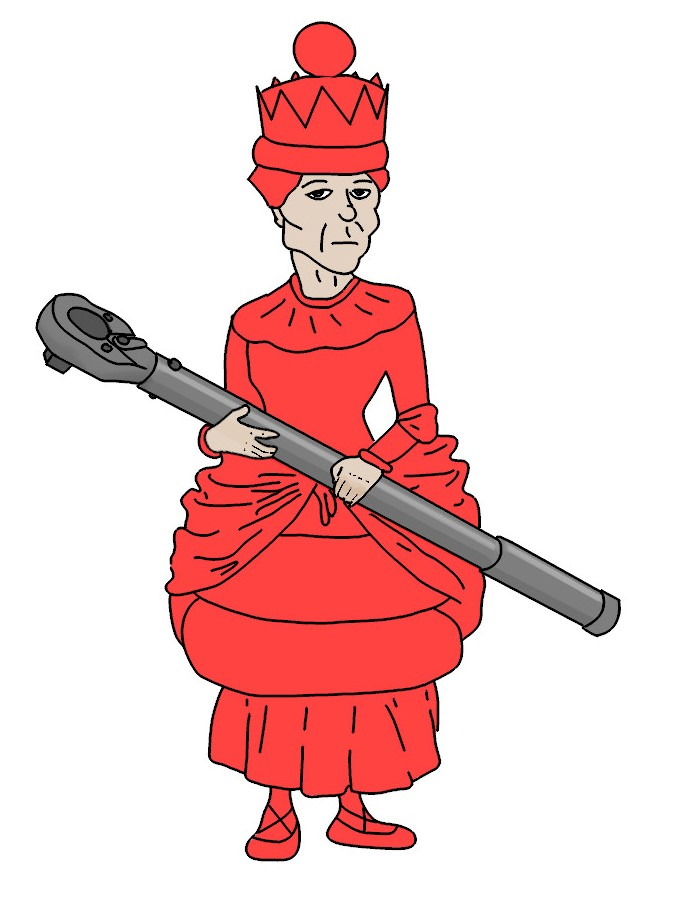
\includegraphics[width=0.35\textwidth,height=\textheight]{images/fig6-1.jpeg}
\end{center}

In 1988, Indiana University advertised for an assistant professor in
population biology with emphasis on disease ecology. Lynda and I both
applied. Happily, we were offered a split position in Biology in which
we each got half salary. It may not sound like a good deal, but we were
thrilled. It is not easy for a dual-career couple in the same field. We
relocated to Bloomington in January 1990, arriving during a cold snap
(-20° C). We moved into a university house, but we did not know enough
to have the electricity turned on before arrival. Luckily, we still had
our down sleeping bags, which we had purchased for field work in the
Southern Alps. Aside from the chilly start, moving to Bloomington was
the beginning of an academic dream come true.

\section{The Problem}\label{the-problem-1}

Since the beginning of my work on sex/asex, there were two things that
worried me about the Red Queen Hypothesis. The first of these was
pointed out by May and Anderson (\citeproc{ref-may1983a}{1983}). This
1983 paper is the same incredible study that launched the wave of
studies on the evolution of parasite virulence, but it was also one of
the first simulation studies of the Red Queen Hypothesis for sex. May
and Anderson concluded that the Red Queen could work, but only if
parasites killed their hosts (i.e., they were maximally
virulent).\footnote{May and Anderson, for example, state, ``Our studies,
  in which the epidemiological details of the parasite--host
  interactions are treated more explicitly than in Hamilton's work, make
  this {[}the parasite{]} answer to the problem of sex
  (\citeproc{ref-ghiselin1974a}{Ghiselin 1974};
  \citeproc{ref-maynard1978a}{Maynard Smith 1978};
  \citeproc{ref-williams1975a}{Williams 1975}) less likely.''} So, it
seemed to me that the Red Queen could not be a general explanation for
sex. It was for this reason that I was biased against the hypothesis
when I first started my work in New Zealand. But as May and Anderson
pointed out, their model made assumptions that were ``not brought down
from Mt. Sinai.'' They assumed, in particular, that infection was
mediated by a single locus with two alleles, giving three genotypes.
They also assumed that the clonal population was initiated with all
three possible genotypes for resistance. These are critical assumptions,
as we will see in Part Two (or see \citeproc{ref-lively2018a}{Lively
2018}).

The second problem was that parasites do not select for sex per se. They
only select against common genotypes. This means that once parasites
drive a common clone down to a rare frequency, it should become favored
by selection. Barring loss of the clone by chance in small populations,
the clone should increase in frequency, eventually leading to
oscillations over time. So, while parasites might prevent the fixation
of the clone in the short term, they do not eliminate it. Now here is
the problem. What if a second clone, with a different genotype, arises
in the population? It should also spread when rare. So should any new
clone. Given that parasites are simply a source of frequency-dependent
selection, parasite-mediated selection should lead to the accumulation
of different clonal genotypes (\citeproc{ref-lively1994a}{Lively \&
Howard 1994}).\footnote{In a computer simulation, a sexual population
  with eight possible genotypes (three locus haploid model with two
  alleles each) was rapidly replaced by two randomly selected clonal
  genotypes. The first clone was introduced at time one, and it began
  oscillating with the sexual population. The second clone was
  introduced at time 100. It began oscillating out of phase with the
  first clone. The sexual population was driven to extinction by
  generation 150 (\citeproc{ref-lively1994a}{Lively \& Howard 1994}).
  Thus, sexual reproduction may not be stable to invasion and
  replacement by a diverse clonal population.} It seemed obvious that,
if clonal diversity became sufficiently high, the diverse clonal
population would eliminate the sexual population. Hence the Red Queen
did not seem stable in the face of repeated mutation to asexual
reproduction. I began to think that combining alternative hypotheses
might be useful. I turned first to Muller's ratchet.

\section{Muller's Ratchet}\label{mullers-ratchet}

Herman J. Muller was a prize-winning geneticist. He won the Nobel Prize
in Medicine and Physiology just one year after moving to Indiana
University in 1945. In the early 1960s, Muller was invited to write an
introductory paper for a new journal. The editor made an effort to
acknowledge Muller in the preface to this first issue
(\citeproc{ref-sobels1964a}{Sobels 1964}): ``We are particularly honored
that we can start the journal with a paper by Dr.~H. J. Muller.'' In
this inaugural paper, Muller (\citeproc{ref-muller1964a}{1964}) wrote a
bomb sentence: ``{[}W{]}e find that an asexual population incorporates a
kind of ratchet mechanism, such that it can never get to contain, in any
of its lines, a load of mutations smaller than that already existing in
its at present least-loaded lines.'' In other words, obligately asexual
populations should accumulate deleterious mutations over time. A decade
later, Joe Felsenstein (\citeproc{ref-felsenstein1974a}{1974}) named the
idea ``Muller's ratchet,'' and he pointed to the probable importance of
the ratchet in population genetics.\footnote{From Felsenstein
  (\citeproc{ref-felsenstein1974a}{1974}): ``I will not attempt here to
  predict from theory the quantitative effect of the ratchet mechanism.
  Involving natural selection, mutation, and genetic drift at many
  linked loci, the problem poses enormous difficulties for the
  application of population genetics theory. But the possible
  significance of the phenomenon makes it important that some
  theoretical treatment should be attempted. The ratchet mechanism has
  been unjustly ignored by theoretical population genetics.''} The
concepts underlying the idea are not especially intuitive, but I will
try to explain the gist of it. First, we must ask, what is a clone?

I have been using ``clone'' so far to describe a group of genetically
identical descendants from a single asexual individual. But Muller knew
that this was not strictly true because mutation happens. Thus, as any
new clone spreads in a population, mutations accumulate, leading to
variation among individuals in the number of mutations
(Figure~\ref{fig-6-1}). It must be true then that there is a group of
individuals within the clone that have the fewest mutations. Muller
called this the ``least-loaded class.'' Here is Muller's insight. Given
that the least-loaded class in a finite population might be a handful of
individuals, the least-loaded (most fit) class could be lost by chance.
How would that happen? Two ways. First, the members of the least-loaded
class (``LLC'') could be lost by bad luck. Maybe all five of members of
the LLC were washed away by a flood, or anything related to being in the
wrong place at the wrong time. Second, the members of the LLC might
produce offspring with one (or more) new mutations. Clearly, the two
options are not mutually exclusive. The point is the least-loaded class
can be lost. This means that the ratchet clicks towards a greater mean
number of mutations in an asexual line.

My students will immediately engage, ``Okay, but the most-loaded class
could also be lost for the same reason.'' Yes, that is correct. But the
most-loaded class can be restored by new mutations in the second
most-loaded class. In contrast, the LLC can only be restored by back
mutation, which has a very low probability of occurrence. Hence, the
mean number of mutations in a clonal lineage is expected to increase
over time, thereby decreasing mean fitness and eroding the advantage to
asexual reproduction.

The ratchet, however, takes a long time to work, especially in large
populations where genetic drift is less problematic. As such, a clone
would likely outcompete and eliminate the coexisting sexual population
before the ratchet drives the clone to extinction. Hence, Muller's
ratchet does not seem to be a viable stand-alone explanation for the
persistence of obligately sexual populations. But what if there were a
force that periodically reduced the number of clonal individuals? That
should increase the rate of mutation accumulation by genetic drift in
the asexual lineage. Hopefully, you can see where this is going.

\section{Synergistic Ideas? The Ratchet and the Red
Queen}\label{synergistic-ideas-the-ratchet-and-the-red-queen}

Here is the idea. Parasite-mediated selection against common genotypes
might prevent the fixation of a clone in the short term. Parasites could
also drive clones through periodic bottlenecks, which would speed up the
rate at which the ratchet clicks. The ratchet could then gradually
reduce the reproductive advantage of asexual reproduction. Eventually
the clone would be eliminated, not by parasites, but by a
parasite-driven ratchet. Perhaps the ratchet could eliminate different
clonal lineages as quickly as they were generated by mutation in the
sexual population.

My first PhD student at Indiana University was Steve Howard, who
transferred in from another lab. Early on, we had many discussions about
our experiences as construction workers and our fondness for characters
in John Steinbeck's books. We also began to expand on the possibility of
synergism between the ratchet and the Red Queen. During one of our
sessions, Steve (in a whimsical moment) said that he could have a
solution in the morning. But it was not an overnight problem to solve,
as we both soon realized. The solution required an individual-based
computer simulation, which was not common at that time
(\citeproc{ref-judson1994a}{Judson 1994}). By that I mean that Steve had
to write a simulation that kept track of every individual in the
population, including whether it became infected, and whether it
produced offspring with one or more new mutations. Steve is a locked-on
theoretician. He could not sleep during the construction of his model,
and he would sometimes call me in the middle of the night. First, he had
to show that the model would converge on analytical solutions for the
number of mutations at equilibrium. This equilibrium is called
``mutation-selection balance,'' which occurs when the input of mutations
is exactly cancelled out by the elimination of mutations by natural
selection (Section~\ref{sec-app-6}). But what is the analytical
solution?

As in any model, there are assumptions involved. For starters, let's
assume that the proportional reduction in fitness caused by each new
mutation is the same as for all previous mutations (independent
effects). Therefore, the fitness of an individual with \(k\) mutations
is given by \((1-s)^k\) where \(s\) gives the selection against each
mutation. Kimura and Maruyama (\citeproc{ref-kimura1966a}{1966}) showed
that the number of mutations at mutation-selection balance is equal to
\(U/s\), where \(U\) is the expected number of new mutations in
offspring. Further, they showed that mean fitness at mutation-selection
balance is equal to \(e^{-U}\), assuming that selection is weak
(Figure~\ref{fig-6-1}). Following Kimura and Maruyama's results, John
Haigh showed further that the number of individuals in the least-loaded
class (\(n_0\)) at mutation-selection balance is: \(n_0=Ne^{-U/s}\)
where \(N\) is the total population size
(\citeproc{ref-haigh1978a}{Haigh 1978}). Keep in mind that the number of
individuals in the least-loaded class (\(n_0\)) is an especially
important value, because the smaller the number, the easier it is to
lose it by drift, resulting in one click of the ratchet. Haigh also
showed that, once the ratchet clicks, the original (Poisson)
distribution of mutations is reset, where the mean of the distribution
is increased by one (Figure~\ref{fig-6-2}). Critically, Haigh's result
suggests that \(n_0\) can be fewer than 10 individuals, even for very
large population sizes. The ratchet seems unavoidable.

\begin{figure}

\centering{

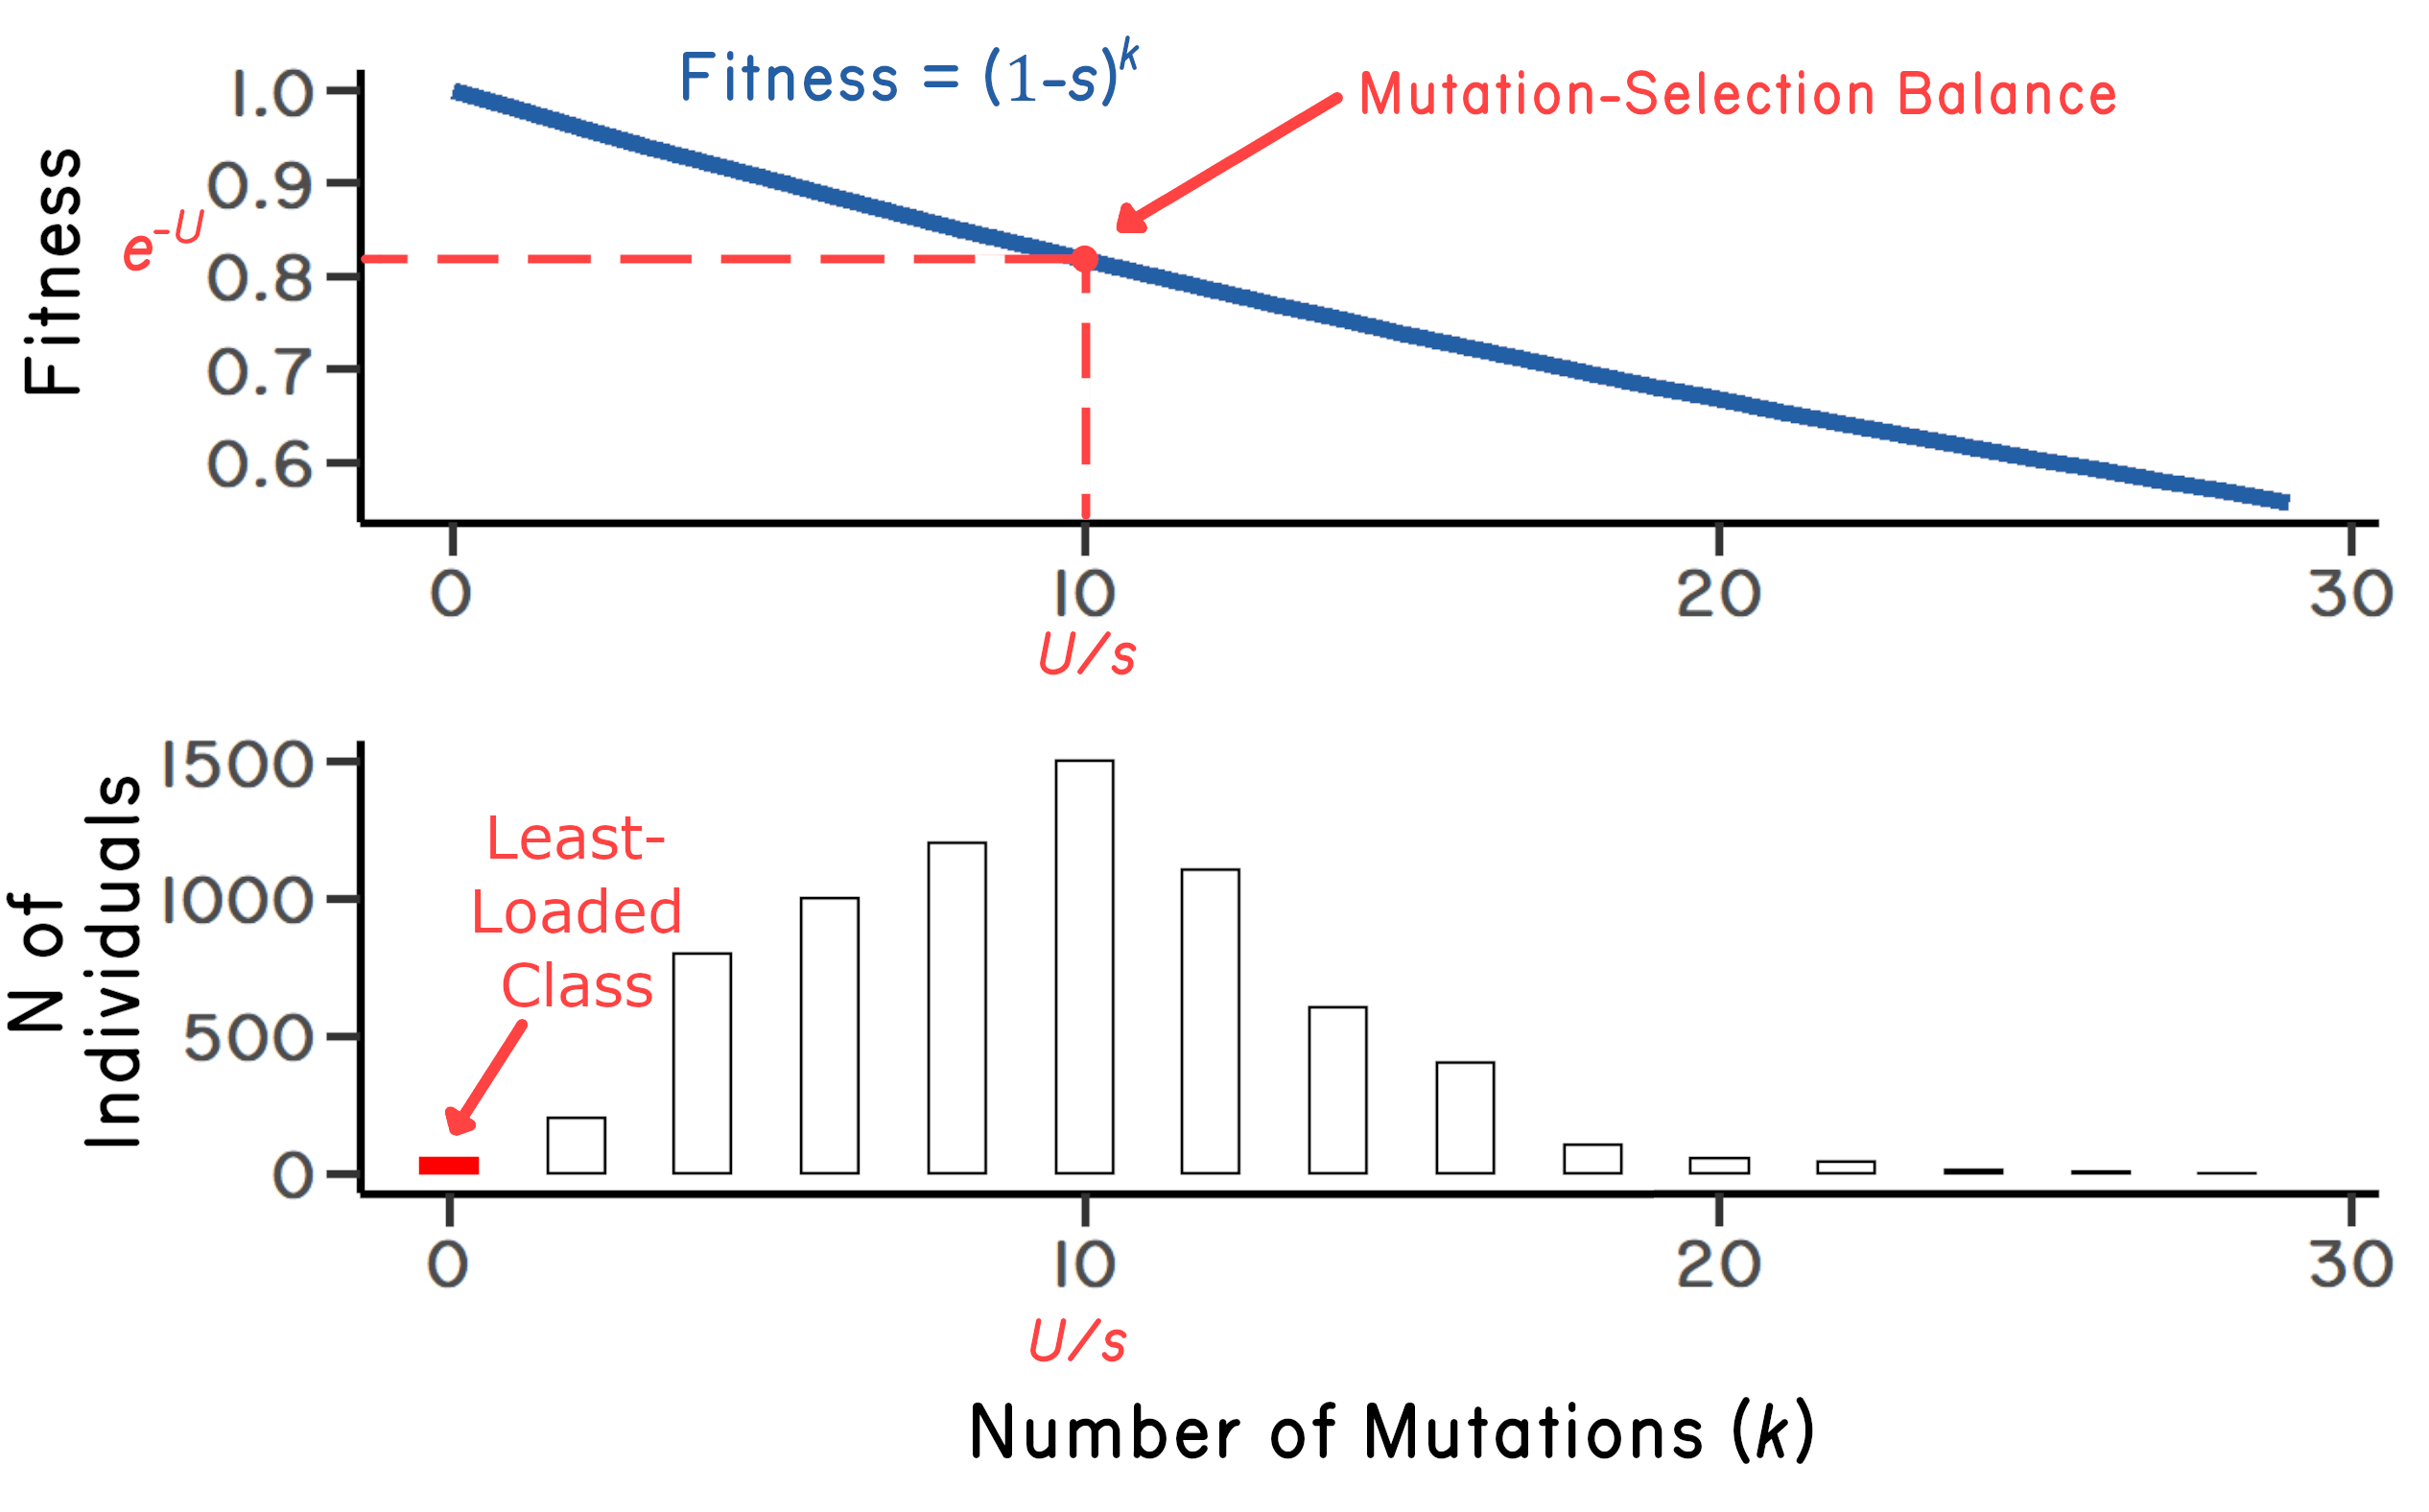
\includegraphics[width=0.8\textwidth,height=\textheight]{images/fig6-2.png}

}

\caption[Fitness as a function of the number of mutations assuming
independent effects \& The distribution of mutations at
mutation-selection balance]{\label{fig-6-1}\textbf{A.} Fitness as a
function of the number of mutations assuming independent effects.
\textbf{B.} The distribution of mutations at mutation-selection balance.
Note that the number of individuals in the least-loaded class is
\(Ne^{-U/s}\), which can be a small number. The ratchet clicks whenever
the least-loaded class is lost by chance.}

\end{figure}%

\begin{figure}

\centering{

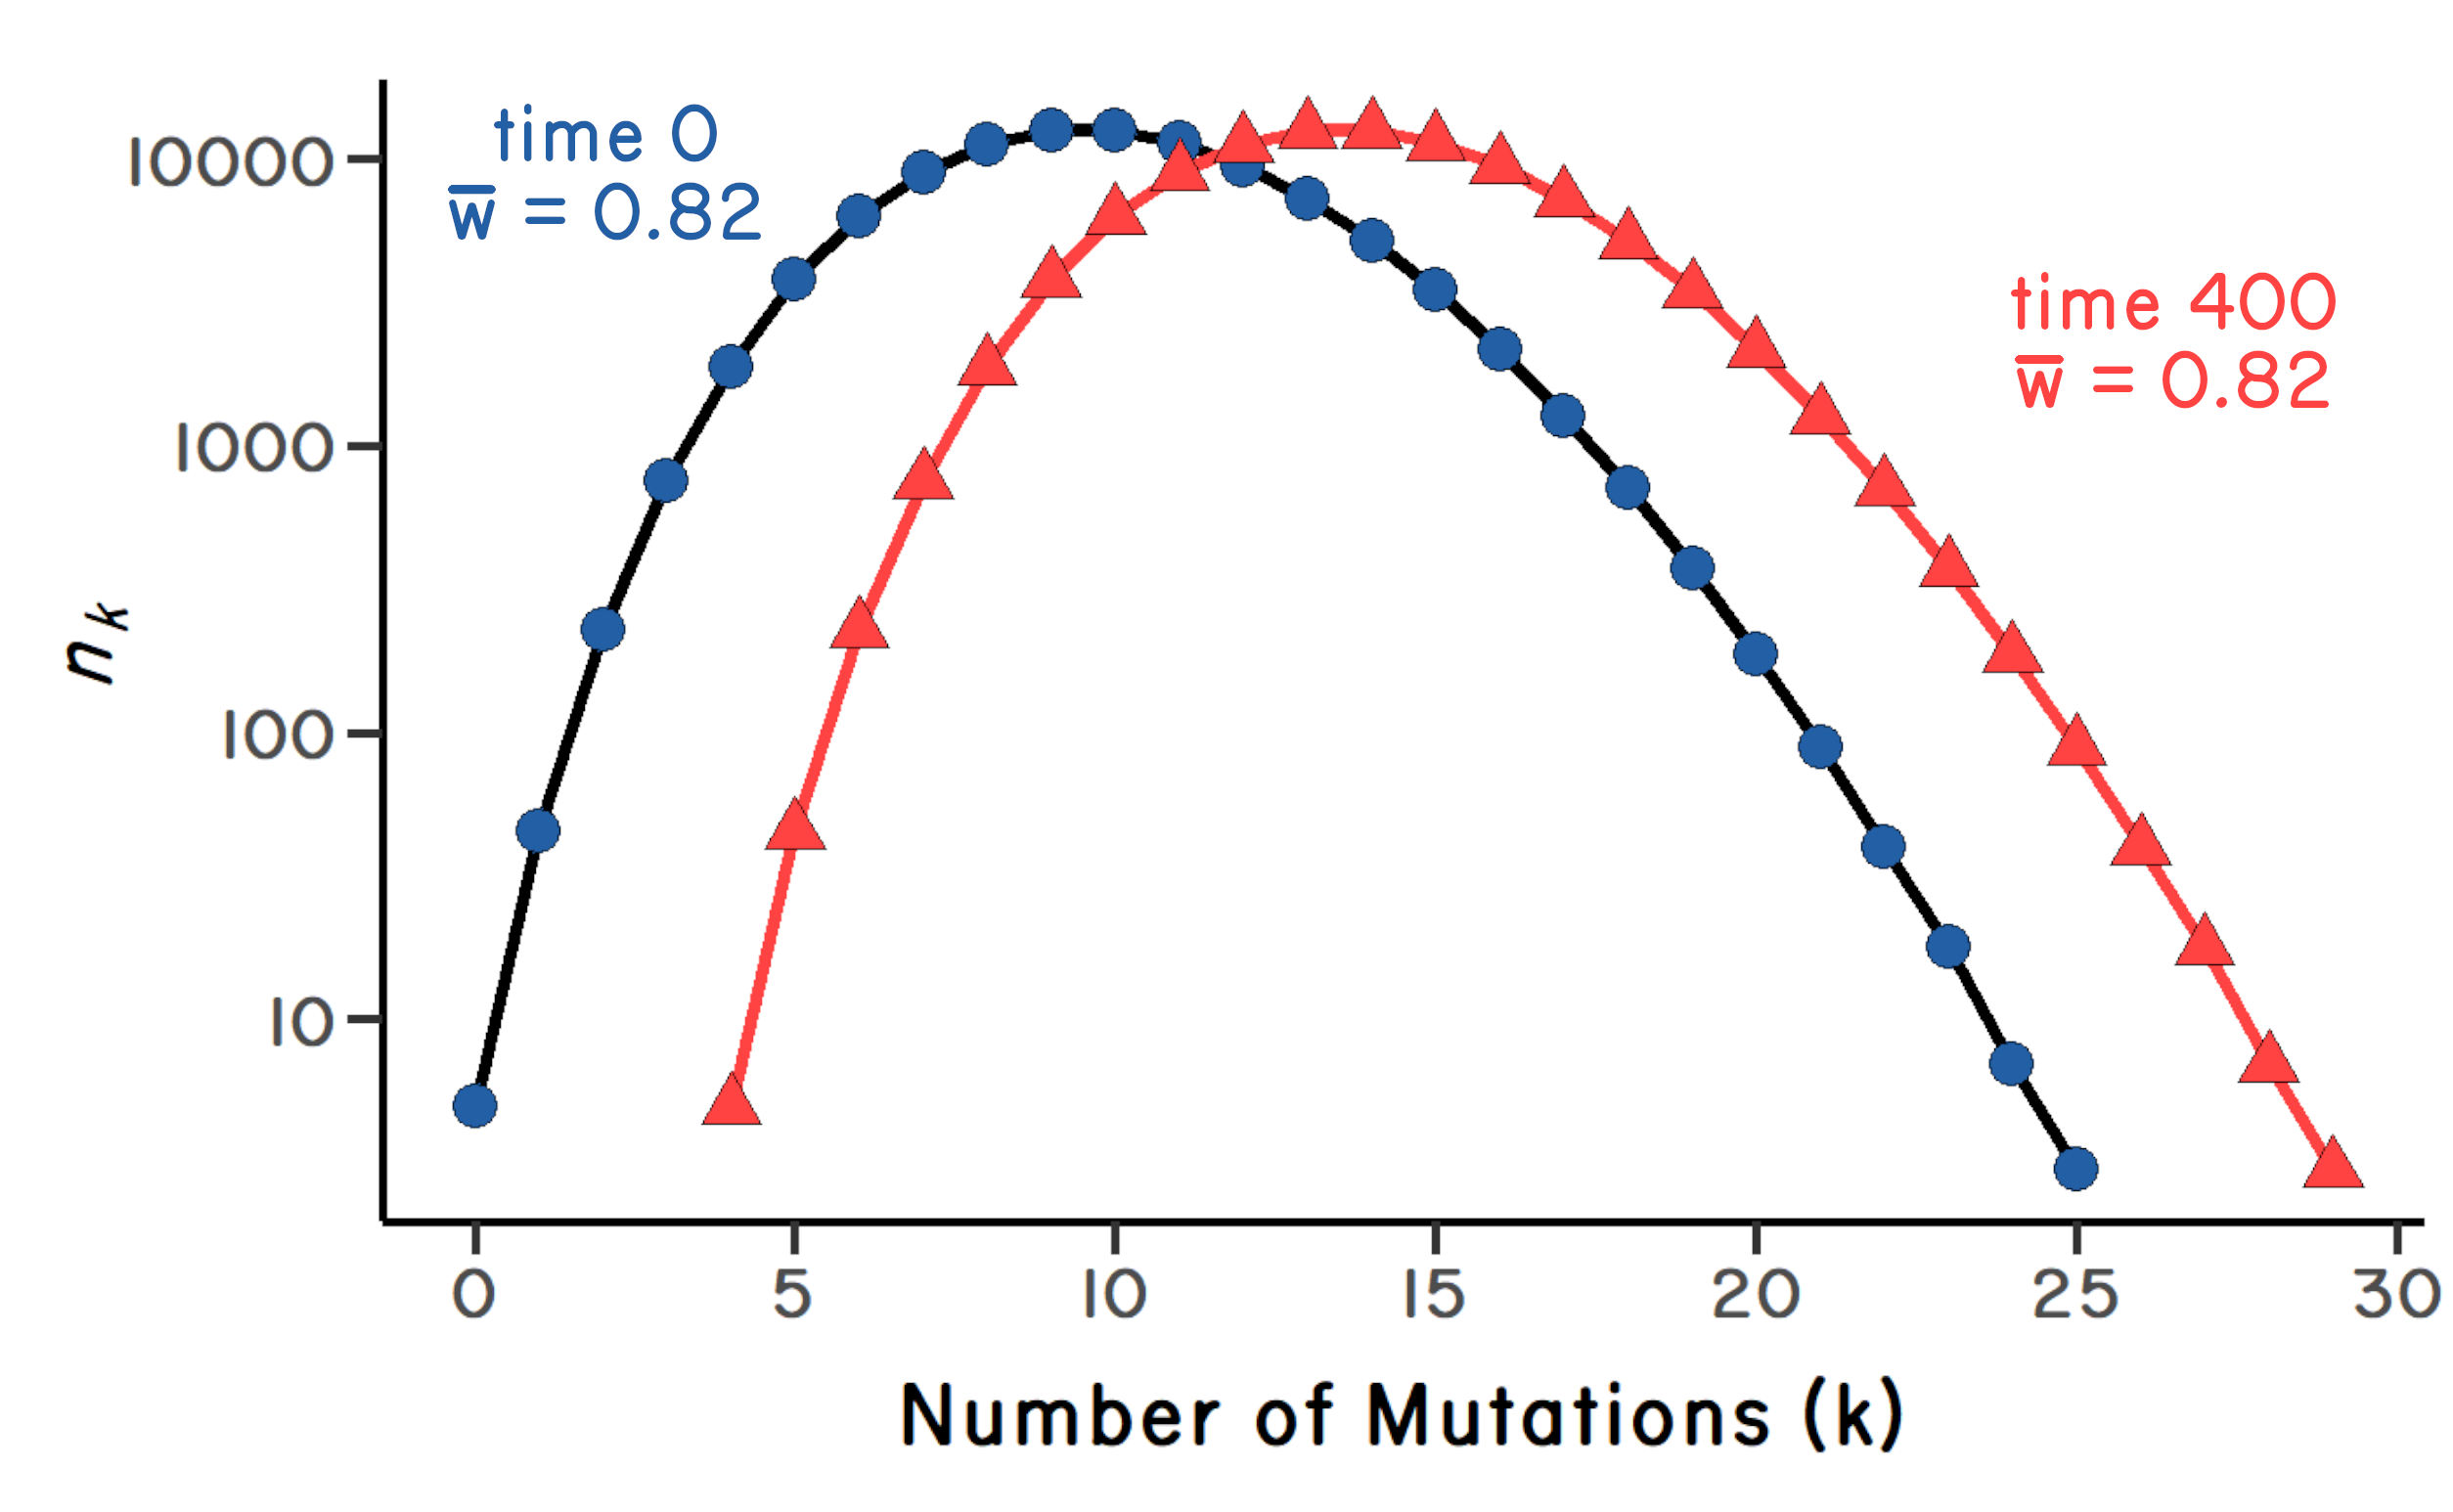
\includegraphics[width=0.8\textwidth,height=\textheight]{images/fig6-3.png}

}

\caption[The distribution of mutations at two time points following
Haigh's simulation results]{\label{fig-6-2}The distribution of mutations
at two time points, following Haigh's (\citeproc{ref-haigh1978a}{1978})
simulation results for \(N = 100,000\), \(s = 0.02\), and \(U = 0.2\).
The blue line shows the distribution of mutational classes before the
operation of the ratchet. The red line shows the distribution after 400
generations, following four clicks of the ratchet. The number of
individuals in the LLC is five at both time points. Mean fitness
(\(\bar{w}\)) is relative to individuals with zero mutations.}

\end{figure}%

Happily, Steve's simulation converged on the analytically derived values
for the mean number of mutations and the mean fitness at
mutation-selection balance. Now for the more difficult part. Does
host-parasite coevolution accelerate the accumulation of mutations in
clonal lineages? Does the combination of the ratchet and the Red Queen
lead to extinction of the clone before it eliminates its sexual
competitors? Note that the simulation made the conservative assumption
that infected individuals in the most-loaded class had the same fitness
as infected individuals in the LLC. In other words, infection was not
more severe in individuals having more mutations.

Steve's simulations showed that, in the absence of parasites, an
initially rare clone went to fixation in fewer than 50 generations,
thereby driving the sexual population extinct
(\citeproc{ref-howard1994a}{Howard \& Lively 1994b}).\footnote{After the
  proofs were corrected and returned, the shading was washed out in
  Figures 1 and 2. Even worse, the panels were reversed for Figure 3.
  The corrected figures were reprinted in Howard and Lively
  (\citeproc{ref-howard1994b}{1994a}).} However, after about 500
generations, the clone also went extinct due to the accumulation of
mutations via the ratchet. Hence, the ratchet was sufficient to take out
the clone, but not before the clone replaced the entire sexual
population. In the presence of parasites, but without the ratchet, the
clone also rapidly replaced the sexual subpopulation, and the clone's
descendants remained at carrying capacity for the duration of the
simulation (Figure~\ref{fig-6-3}).

\begin{figure}

\centering{

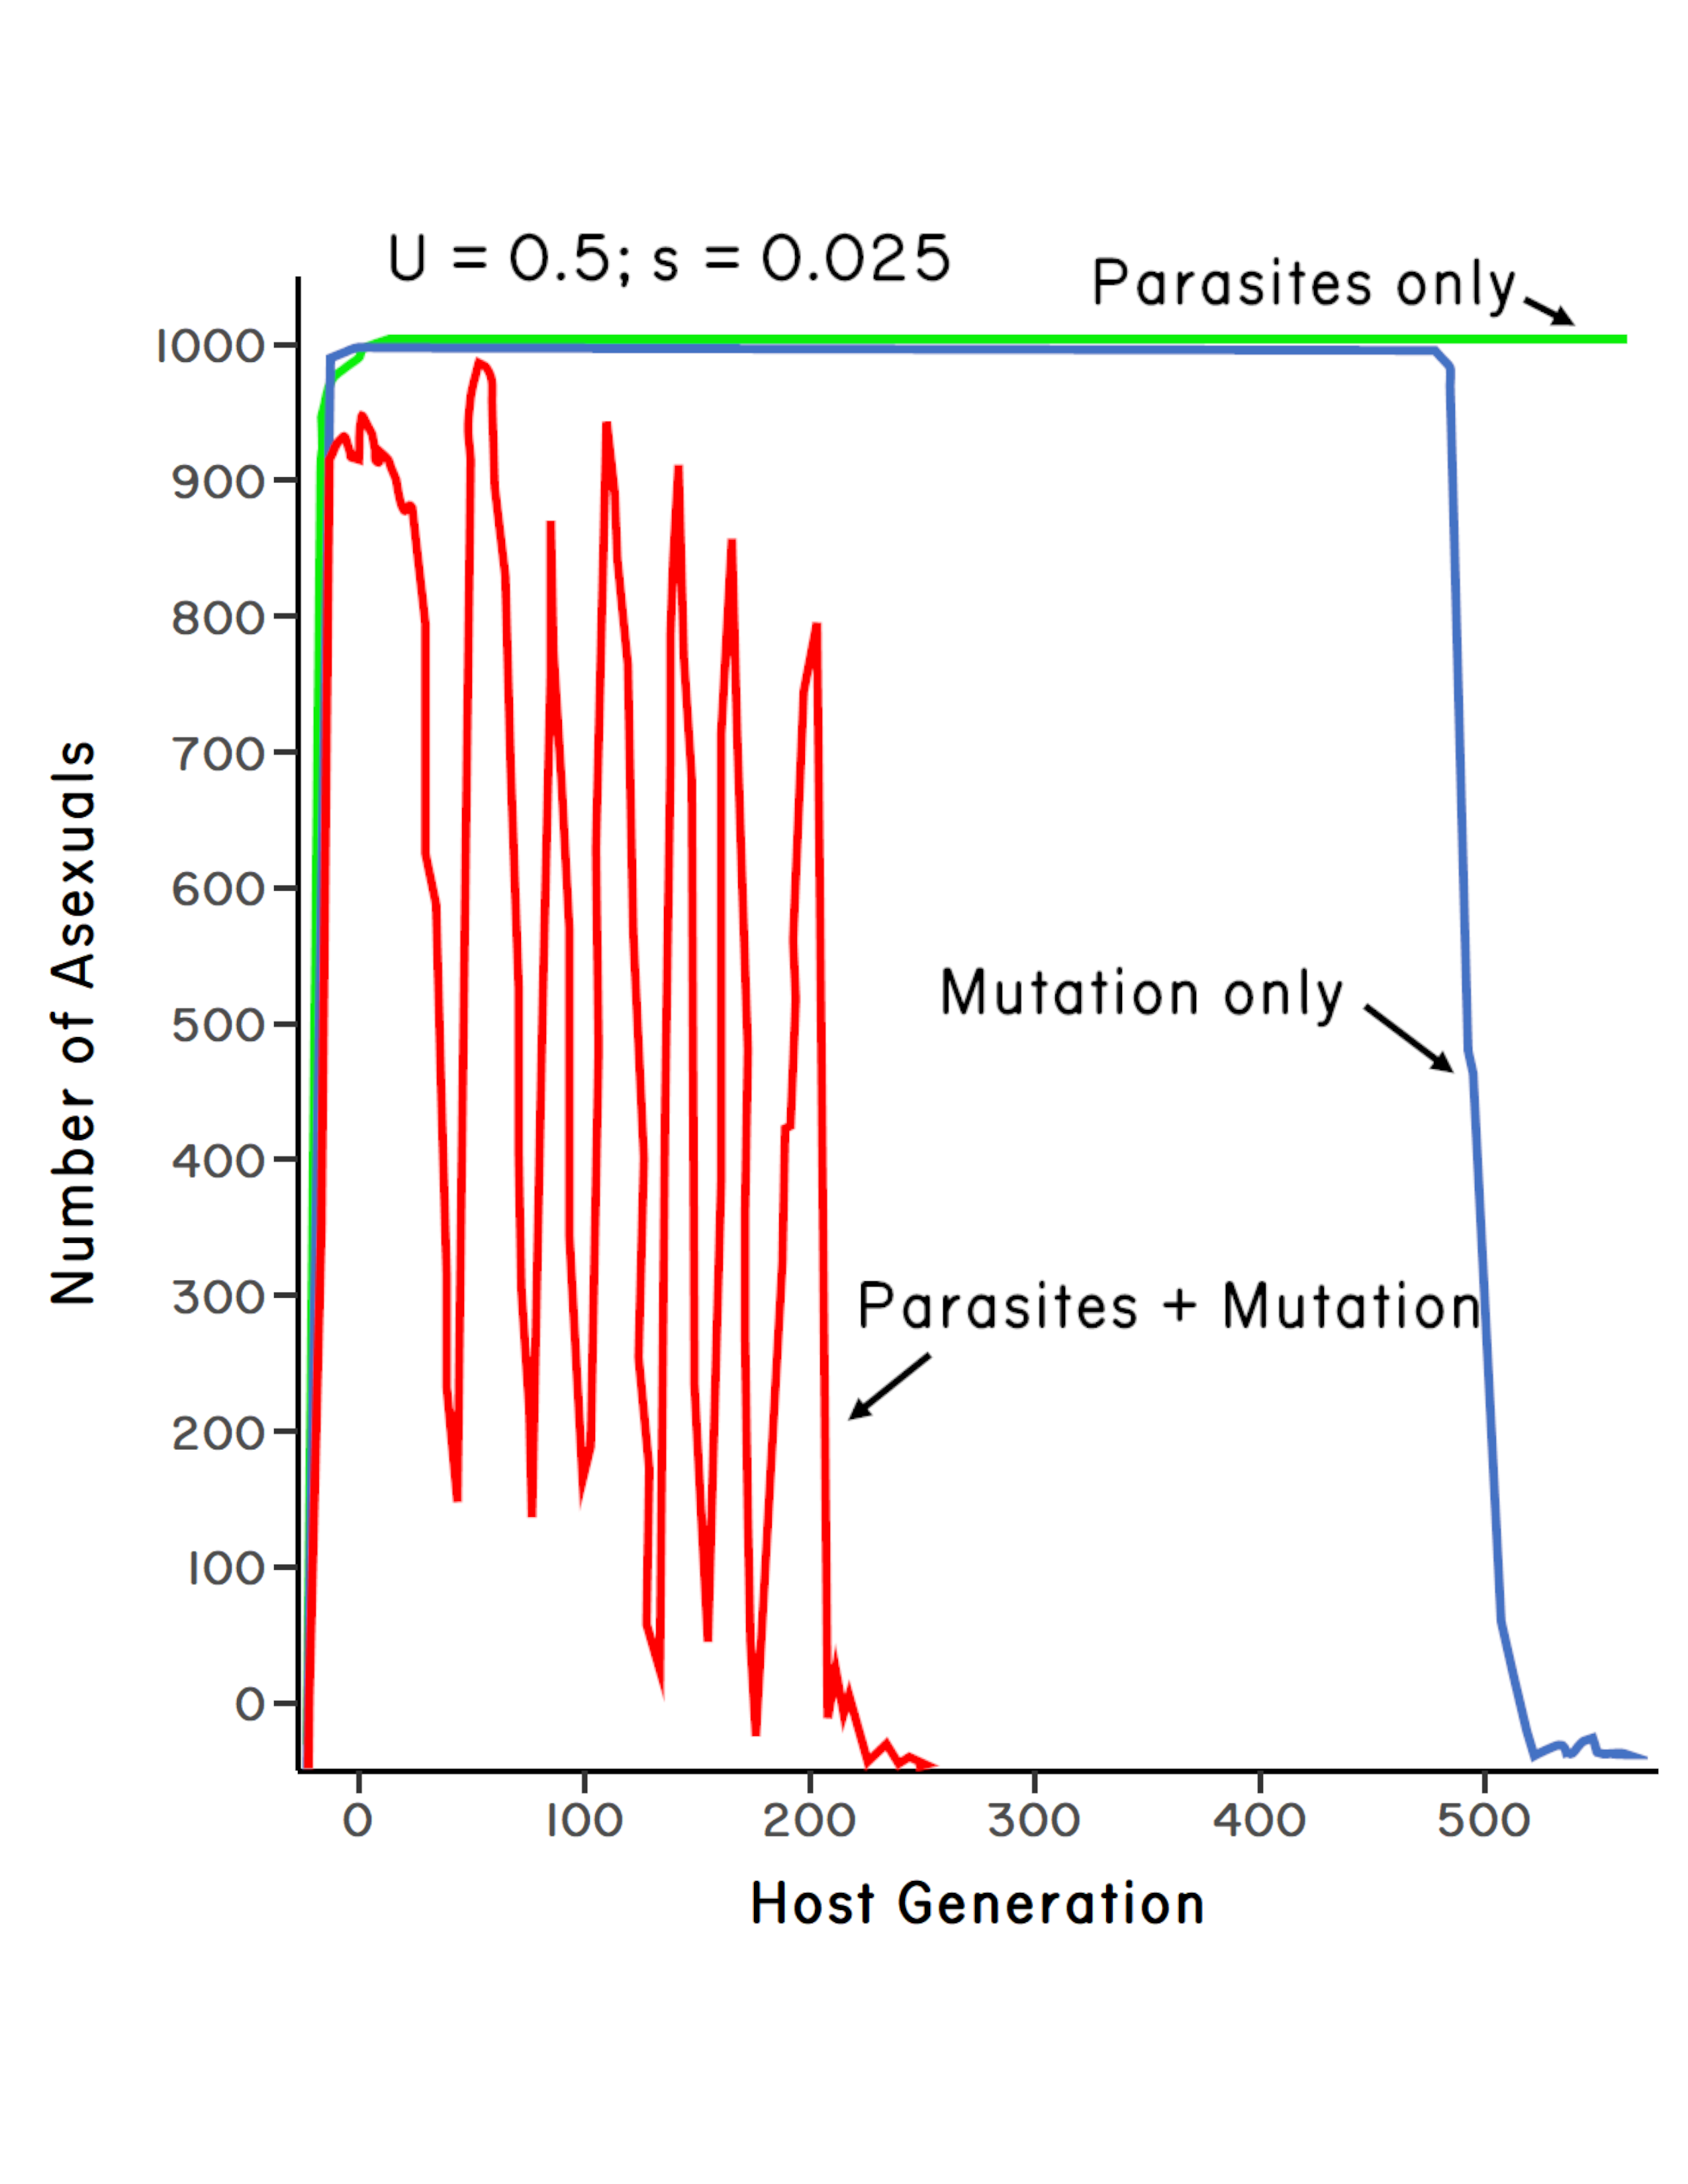
\includegraphics[width=0.6\textwidth,height=\textheight]{images/fig6-4.png}

}

\caption[Representative simulation
results]{\label{fig-6-3}Representative simulation results. The green
line shows a simulation for hosts infected with coevolving parasites,
but in the absence of deleterious mutations. Virulence and transmission
were both moderate (\(= 0.5\)). Under these conditions, the sexual hosts
were eliminated by the clone. The blue line shows a case without
parasites in which mutations occur with a probability of 0.5 per genome
per generation \((U = 0.5)\), and selection against mutation is
\(s = 0.025\). Again, the clone goes to fixation, but it is later
eliminated by Muller's ratchet. The red line shows a case where both
mutations and coevolving parasites were included. Here, the clone did
not replace the sexual population but rather oscillated in frequency,
which led to more rapid mutation accumulation and elimination of the
clone. Redrawn from Howard and Lively
(\citeproc{ref-howard1994b}{1994a}).}

\end{figure}%

By contrast, when parasites were combined with the ratchet, sexual
reproduction was initially invaded by the clone, but the clone did not
replace the sexuals. How does that work? The clone was initiated with a
small number of individuals (\(N = 20\)) at mutation-selection balance.
The clone then increased when rare, but as the clone spread in the
population, the ratchet was already working to reduce the two-fold cost
of males (see Chapter~\ref{sec-why-sex}). In addition, as the clone
became common, the parasite population rapidly evolved to infect it.
This combination of the ratchet and parasite-mediated
frequency-dependent selection prevented the clone from fixing in the
short term. The clone then began to oscillate in frequency over time.
But every time the clone was driven to low frequency, the number of
individuals in the LLC decreased, thereby allowing for a more rapid
operation of the ratchet. Notably, over the period of several
oscillations, the clone tended to be driven to lower frequencies each
time. So as the ratchet erodes the cost of males, the clone was driven
to a lower frequency during successive oscillations, which fed back to
fuel the ratchet. The clone is toast. Eventually the clone undergoes a
mutational meltdown and goes extinct (\citeproc{ref-lynch1990a}{Lynch \&
Gabriel 1990}).\footnote{Mutational meltdown in clones occurs when their
  intrinsic birth rates are near one, meaning that the females are just
  barely replacing themselves. This then keeps the clonal population
  small, which also keeps the least-loaded class small, thereby aiding
  the ratchet. Once the intrinsic birth rate drops below one, the clone
  will go extinct.} This example provides a proof of concept that
host-parasite coevolution can work in a synergistic way with Muller's
ratchet to prevent fixation of the clone in the short term (\textless20
generations) and to ensure the elimination of the clone in the longer
term.

To get a better feeling of the parameter space over which the ratchet
and the Red Queen could work to select for sex over the long term, Steve
explored different combinations of mutation rate, selection against
mutation, parasite virulence, and parasite transmission. In the absence
of mutation, the results showed that sexual reproduction was
evolutionarily stable only when parasites were both extremely virulent
and highly transmissible (Figure~\ref{fig-6-4}). This result was
consistent with the model of May and Anderson
(\citeproc{ref-may1983a}{1983}). Sexuals and asexuals coexisted where
parasite virulence and transmission were both high, but not at maximum
values (Figure~\ref{fig-6-4}). Finally, asexual reproduction replaced
sexual reproduction when parasites had low levels of virulence and/or
transmission.

\begin{figure}

\centering{

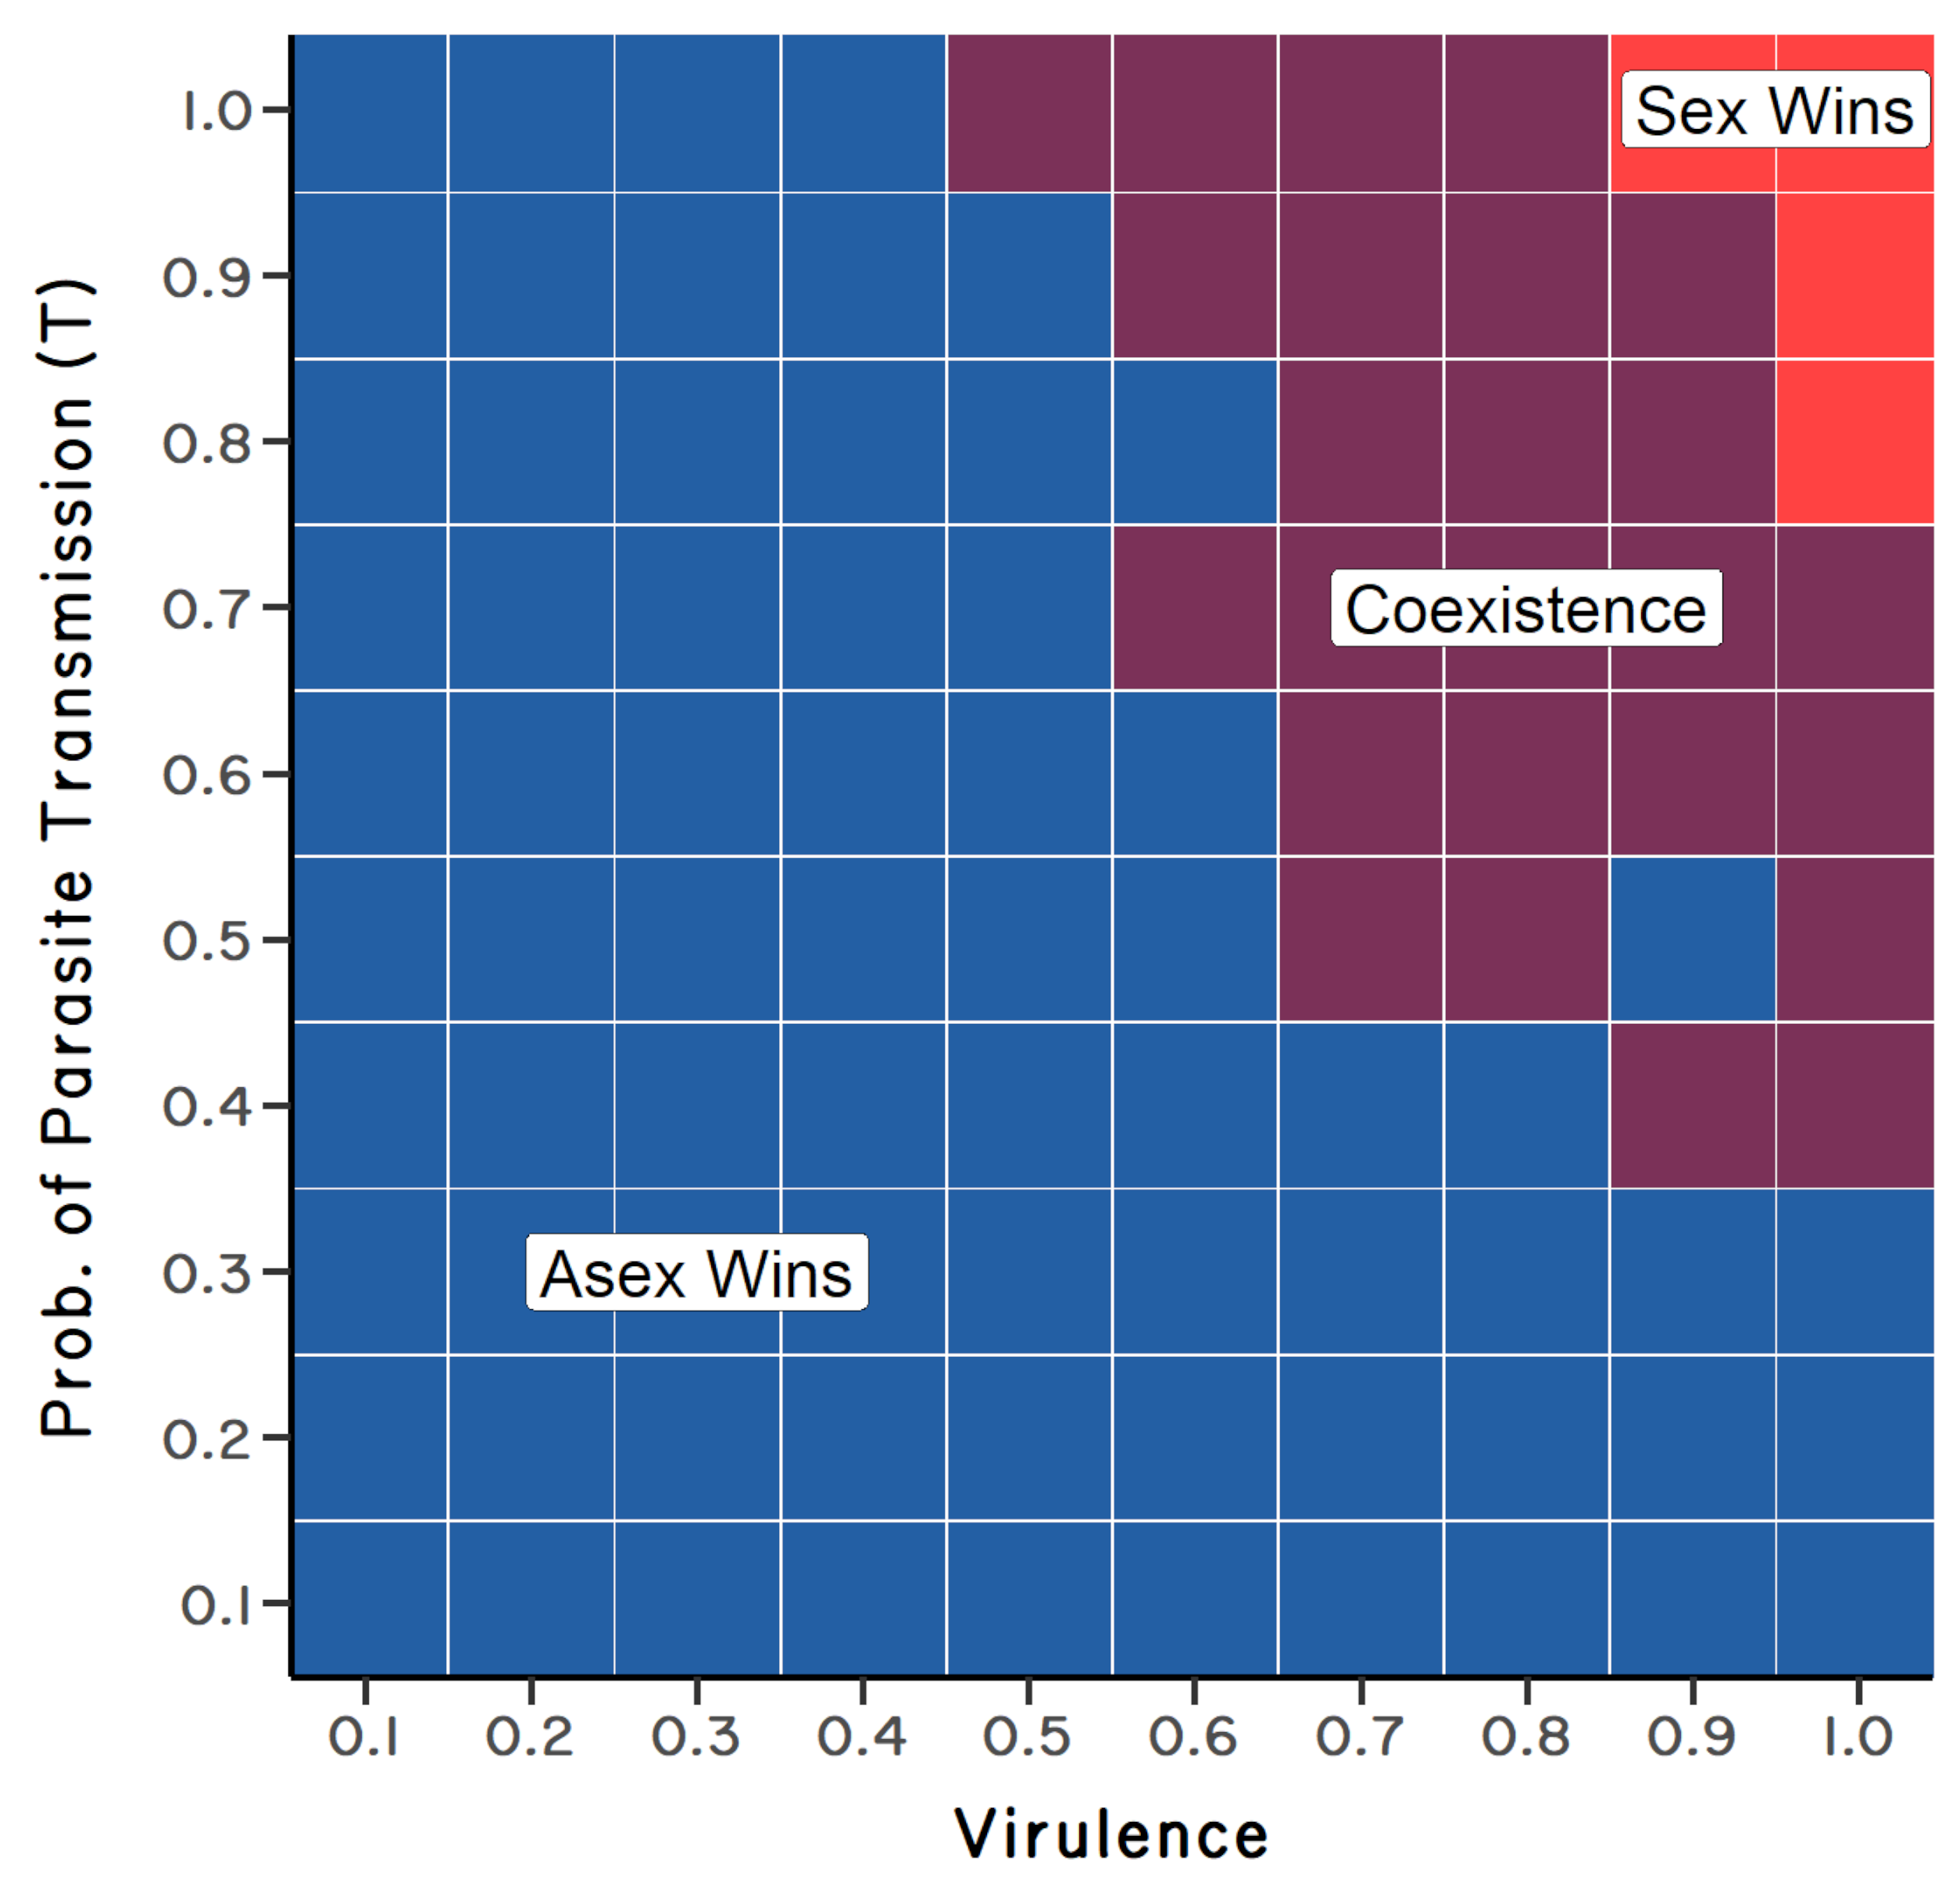
\includegraphics[width=0.6\textwidth,height=\textheight]{images/fig6-5.png}

}

\caption[Parameter space showing regions where sexual reproduction
persists in the face of competition with a single clone in the absence
of mutation]{\label{fig-6-4}Parameter space showing regions where sexual
reproduction persists in the face of competition with a single clone in
the absence of mutation. Note that sexual reproduction only wins
outright when virulence is at or near its maximum value of one and
transmission is also very high. Asexual females replace sexuals at low
levels of transmission and virulence. Finally, there is an intermediate
zone on the virulence-transmission axis where sexual and asexual females
coexist. Redrawn from Howard and Lively
(\citeproc{ref-howard1994b}{1994a}).}

\end{figure}%

Now, what if we add in mutation? Steve's results suggested that for
genome-wide mutation rates of \(U = 0.5\) to \(1.0\), sexual
reproduction was stable to replacement by asexual reproduction, even
when parasites \textbf{were only moderately virulent}.\footnote{``Virulence''
  is defined here as the effect that infection has on host fitness. For
  example, a virulence value of 1.0 indicates that infection kills or
  sterilizes the host. A virulence of 0.1 indicates that infection
  reduces host fitness by 10\%.} This surprised us! One of the major
difficulties for the Red Queen had been that May and Anderson's
(\citeproc{ref-may1983a}{1983}) results suggest that parasites had to
kill or sterilize infected hosts to provide sufficiently strong
selection for cross-fertilization. Steve's new results suggested that,
in combination with the ratchet, parasites did not have to generate such
strong selection against infected individuals (Figure~\ref{fig-6-5}).
When we started out, we had not imagined that the synergism between the
ratchet and the Red Queen could be so powerful.\footnote{Steve followed
  this initial study with a simulation study of mutation accumulation in
  a Red Queen world but changing the assumption from independent effects
  of mutations to synergistic effects of mutations
  (\citeproc{ref-howard1998a}{Howard \& Lively 1998}). The results were
  similar, provided the clonal population has not come into
  mutation-selection balance.}

\begin{figure}

\centering{

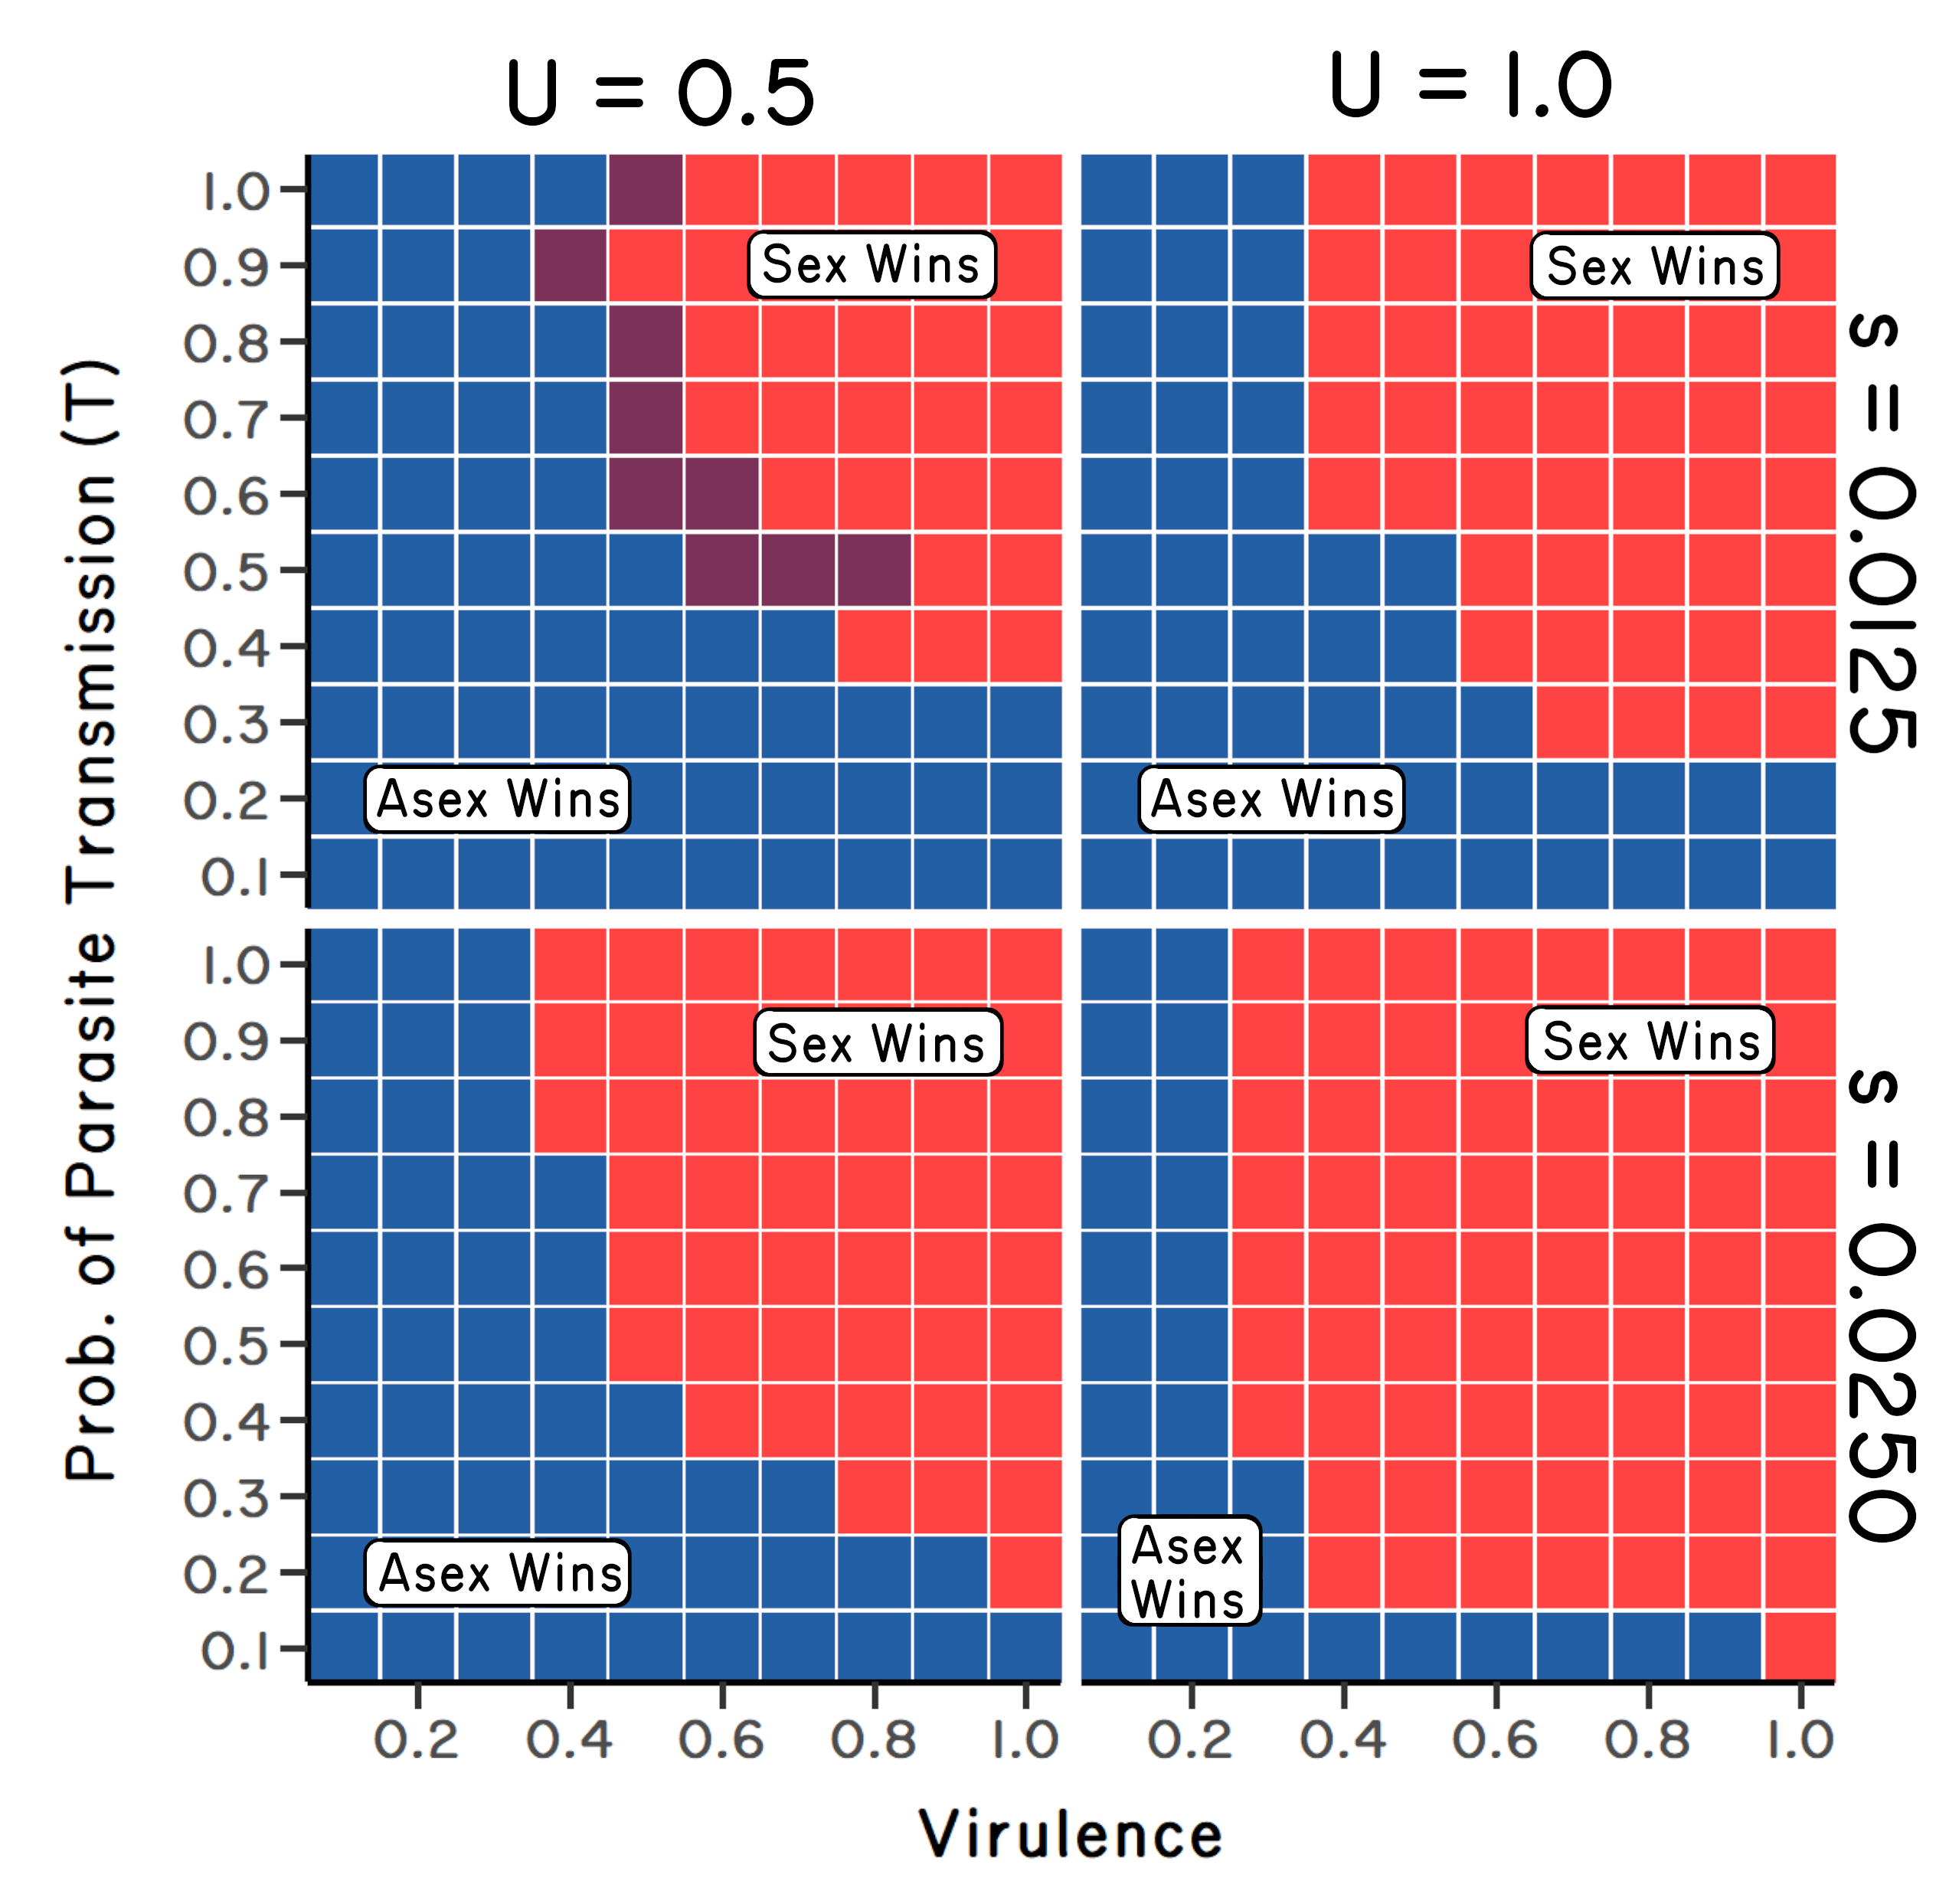
\includegraphics[width=0.7\textwidth,height=\textheight]{images/fig6-6.png}

}

\caption[Parameter space showing regions where sexual reproduction
persists in the face of competition with a single clone in the presence
of mutation]{\label{fig-6-5}Parameter space showing regions where sexual
reproduction persists in the face of competition with a single clone in
the presence of mutation. In comparison to the case without mutation
(Figure~\ref{fig-6-4}), sexual reproduction is stable over a much wider
range of values for transmission and virulence. The zone of coexistence
is also greatly reduced (purple squares). Redrawn from Howard and Lively
(\citeproc{ref-howard1994b}{1994a}).}

\end{figure}%

The potential for synergism between antagonistic coevolution and
mutation accumulation later became the subject of a target review in
1999, headed up by Stuart West (\citeproc{ref-west1999a}{1999}). Stu was
a post-doc in Andrew Read's lab in Edinburgh while I was there as a
sabbatical visitor in the lab. But the whole thing originally started at
a meeting we all attended at the Max Planck Institute in Seewiesen,
Germany. It was an amazing gathering on the evolution of sex, organized
by Nico Michiels, with an incredible mix of faculty, post-docs, and
students. I presented some of the snail data along with the results of
Howard and Lively (\citeproc{ref-howard1994a}{1994b}) to a rather mixed
reaction. To my mind, it seemed that the students and post-docs
(including Stu) liked the idea of combining hypotheses, but at least one
of the more established members in the field saw it as an attempt by
hippies to make everyone happy.\footnote{I heard this kind of thing
  called ``group-hug pluralism'' at a meeting of philosophers in Berlin
  in 2022. In any case, our fusion of the ratchet and the Red Queen was
  based on logic rather than any sort of craving for hugs.} In any case,
Stu expanded on the basic idea back in Edinburgh, and he convinced
Andrew and me to help him craft it as a target review for the
\emph{Journal of Evolutionary Biology}. I was very reluctant, as several
key researchers in the field would be asked to publish their thoughts on
the matter, which I knew were unlikely to be uniformly positive. In the
end, our paper was published---along with over a dozen commentaries (see
\href{https://onlinelibrary.wiley.com/toc/14209101/1999/12/6}{vol.~12,
issue 6}). The commentaries were more positive on average than I
expected, but mainly it was interesting to see the diversity of thought
by some of the top biologists studying sex and recombination at the
time.

My work with Steve Howard on synergism between the ratchet and the Red
Queen led me to rethink my views on Strong Inference, as discussed in
Chapter~\ref{sec-eco-hyp-cont}, where the goal is to force competing
hypotheses to make different predictions before getting the data. But
what if the answer is some combination, or even synergism, between
hypotheses? It could be that forcing predictions could result in the
rejection of all alternatives, when in fact two or more hypotheses were
partially true. And if two hypotheses are strongly synergistic, would it
be appropriate to claim that one was more important? In studying this
problem, I found an excellent article contrasting Platt's strong
inference with Chamberlin's method of multiple working hypotheses
(\citeproc{ref-elliott2007a}{Elliott \& Brook 2007}). Elliott and Brook
state that the two methods are often treated as the same idea (of which
I was guilty in Chapter~\ref{sec-eco-hyp-cont}). But they are not the
same. Platt's paper (which drew heavily from Chamberlin) focused on
designing programs that would falsify all but one of the alternatives,
whereas Chamberlin allowed for combinations, and even synergism, between
competing hypotheses. It now seems to me that Chamberlin's
(\citeproc{ref-chamberlin1890a}{1890}) paper better describes the best
way forward with respect to the problem of sex.

\subsection{What about parasites?}\label{what-about-parasites}

One of the major patterns of sex/asex was pointed out by Graham Bell. He
found that parasitic species were much more likely to be outcrossing
than their free-living relatives (\citeproc{ref-bell1982a}{Bell 1982}).
This finding was emphatically supported by a formal phylogenetic study
of free-living versus parasitic nematodes
(\citeproc{ref-gibson2015a}{Gibson \& Fuentes 2015}). However, much of
the theoretical focus for sex/asex has focused on hosts. What about
parasites? If host-parasite coevolution can contribute to selection for
sexual reproduction in hosts, does it also feedback to select for sex in
parasites? If so, is it sufficient? Steve Howard was one of the first
theoreticians to address these questions along with Alison Galvani and
Katrina Lythgoe (\citeproc{ref-galvani2003a}{Galvani \emph{et al.}
2003}; \citeproc{ref-lythgoe2000a}{Lythgoe 2000}). Steve's results
showed that sexual populations of obligate parasites could be invaded
and replaced by a diverse population of clonal parasite genotypes. More
specifically, repeated mutation to asexual reproduction in the parasite
population led to a diverse clonal population, which eventually replaced
the ancestral sexual population. However, the ratchet, in combination
with Red Queen dynamics, could lead to the elimination of clones and the
long-term maintenance of sexual parasite populations
(\citeproc{ref-howard2002a}{Howard \& Lively 2002}). Hence, the results
for parasites mirror those found for hosts, except that the ratchet
worked more rapidly in obligate parasites, as selection is stronger,
giving rise to more extreme oscillations during Red Queen dynamics. It
is still unknown whether the ratchet and the Red Queen work
synergistically to select for sex in either parasites or
hosts.\footnote{Professor Hamilton told me at a meeting in London that
  he thought combining the ratchet and the Red Queen made sense, but
  that he did not think the ratchet was a necessary addition. See also
  the dissertation work by Olivia Judson for a detailed theoretical
  study of coexistence between sexuals and asexuals in a metapopulation
  (\citeproc{ref-judson1997a}{Judson 1997}).} But it seems like a
sensible possibility, especially where both host and parasite genetic
diversity is very high, host populations are finite, and parasites
rarely coinfect the same host individual. It is also possible, of
course, that neither coevolution nor mutation accumulation is required.
More empirical and theoretical work is required.

\section{Summary}\label{summary-4}

\begin{enumerate}
\def\labelenumi{\arabic{enumi}.}
\tightlist
\item
  The Red Queen Hypothesis is a potentially general way of explaining
  why clonal lineages don't rapidly replace sexual competitors in the
  short term.
\item
  But any source of frequency-dependent selection (such as parasites or
  niche competition) would seem insufficient by itself to eliminate
  clones when rare. However, the elimination of rare clones could be
  aided by either demographic stochasticity in finite populations and/or
  by Muller's ratchet.
\item
  In the case of Muller's ratchet, parasite-mediated frequency-dependent
  selection could facilitate the ratchet-like mechanism by periodically
  reducing the size of the clonal population, thereby increasing the
  rate of mutation accumulation.
\item
  The ratchet/Red Queen idea is very difficult to test, but data for
  \emph{P. antipodarum} suggest that long-lived clonal lineages are most
  likely in populations that are relatively parasite free
  (\citeproc{ref-neiman2005a}{Neiman \emph{et al.} 2005}).
\end{enumerate}

\section{Appendix: Down the Ratchet Hole}\label{sec-app-6}

Suppose the probability of a new mutation in offspring is \(0.5\).
Clearly, it would not make sense to say that every offspring acquires
one half of one mutation. But it would make sense to say that offspring
have a Poisson distribution of new mutations. Under a Poisson
distribution, the frequency of individuals with \(k\) new mutations is
given by \[f_k=\frac{e^{-U}U^k}{k!}\] where \(U\) is the probability of
a new mutation per generation. Under this formulation, the frequency of
offspring that contain no new mutations is given by \[f_0=e^{-U}.\]

Suppose a clonal population begins with a single individual with zero
mutations (\(k = 0\) and \(w_0 = 1\)). As above, let all future
offspring acquire an average of \(U\) additional mutations per
generation. The lineage would gain mutations over time, until the input
of mutations is equal to the loss of mutations due to selection. At this
point in time, the clonal population is at mutation-selection balance.
Kimura and Maruyama (\citeproc{ref-kimura1966a}{1966}) showed that the
average number of mutations in a clonal lineage at mutation-selection
balance is equal to \(U/s\), where \(s\) is the selection coefficient
against each mutation. They also showed that the mean fitness at this
balance (assuming that \(s\) is small) is \[\hat{w}=e^{-U}.\] Hence,
population mean fitness at equilibrium is expected to be equal to the
expected frequency of zero new mutations in offspring.

In an infinite population, we would expect the mean fitness to remain at
this equilibrium value. But populations are finite, which leads to
Muller's ratchet. John Haigh (\citeproc{ref-haigh1978a}{1978})
constructed the first model to deeply explore the ratchet. He first
assumed that each deleterious mutation results in the same proportional
reduction in fitness as all previous mutations. Let \(s\) be the
selection coefficient against each mutation. Under Haigh's assumption,
an individual with zero mutations would have a relative fitness of
\(1\), while an individual with one mutation would have a relative
fitness of \((1-s)\), and an individual with two mutations would have a
relative fitness of \((1-s)(1-s)\). More generally, an individual with
\(k\) mutations would have a relative fitness of \[w_k=(1-s)^k.\] Haigh
assumed that the number of \emph{individuals} having \(k\) mutations
\((n_k)\) at mutation-selection balance also follow a Poisson
distribution, such that
\[n_k=\frac{n_0\left(\frac{U}{s}\right)^k}{k!}.\] In this expression,
\(n_0\) is the number of individuals with zero mutations, which is the
least-loaded class. How many individuals in the least-loaded class? Let
\(N\) be the total number of individuals in the clonal population. Under
a Poisson distribution for mutational load, the number of individuals in
the least-loaded class is \[n_0=Ne^{-U/s}\] where \(e^{-U/s}\) is the
frequency of individuals in the zero class. This means that the LLC can
be quite small, even in large clonal populations. For example, let
\(N = 100,000\), let \(s = 0.02\), and let \(U = 0.2\). Plugging these
values into the solution for \(n_0\) we find that only five individuals
would be in the LLC at mutation-selection balance. Such a small group is
at risk of loss by genetic drift.

Haigh ran simulations to study the loss of the LLC, and the effect of
this loss on the distribution of mutational classes. He found that
following the loss of the LLC, the entire distribution shifted to a
greater mean number of mutations, but the shape of the distribution
remained constant. Hence, after one click of the ratchet, the LLC still
had about five individuals, but now the LLC had one additional mutation.
The mean number of mutations had also increased by one.

\bookmarksetup{startatroot}

\chapter{Overview and Future
Directions}\label{overview-and-future-directions}

\begin{center}

\includegraphics[width=0.37\textwidth,height=\textheight]{images/fig7-1.png}
\end{center}

\emph{``{[}A{]}nd what is the use of a book,'' thought Alice, ``without
pictures or conversations?''}\\
--Lewis Carroll, \emph{Alice's Adventures in Wonderland}

\section{Overview of Key Points}\label{overview-of-key-points}

The main goal of this first volume is to illustrate the perplexing
problem of sexual reproduction. The gist of the paradox is that sex is
costly, but common. Here I focus on the intrinsic cost of producing
males, which arises in sexual populations when competing with
parthenogenetic females. The problem is that sexual females produce
males and females, but males do not directly produce offspring. Thus,
the production of males reduces the per-capita number of births in the
sexual population. If sexual females produce a one-to-one
(male-to-female) sex ratio, a clonal lineage would be expected to double
in frequency when rare and then rapidly replace the sexual individuals
living in coexistence. This argument assumes that sexual and asexual
females are equally fecund and their offspring have equal expectations
for survivorship and reproduction. This is the well-known ``all else
equal'' assumption used by Maynard Smith to build his model. If the
sex-ratio is female-biased in the sexual population, then the clone will
still replace the sexual population, but the rate of replacement is
slower (Figure~\ref{fig-1.2}).

One possible explanation for the persistence of sexual populations is
that the all-else-equal assumption is incorrect. If, for example,
asexuals intrinsically produce fewer than half of the surviving
daughters per capita as sexual females, then asexual mutants will be
eliminated by selection even in stable environments where resources are
abundant and biological enemies are absent. A more interesting
possibility for the persistence of sexual reproduction is that
ecological factors reduce the fecundity and/or survivorship of
parthenogenetic females. This idea makes sense to some degree. The
problem is that for a two-fold cost of males, the ecological factors
must reduce the daughter production of asexual females to fewer than
half that of sexual females. That requires very strong natural
selection.

In Chapter~\ref{sec-eco-hyp}, I reviewed three ideas for why sexual
reproduction might be stable against replacement by parthenogenetic
females (following \citeproc{ref-bell1982a}{Bell 1982}). The first of
these, the Lottery Model, proposes that sexual reproduction is favored
in fluctuating abiotic environments. For example, a clone that is
adapted to cold/dry conditions might not survive following a change to
hot/wet conditions. On the other hand, it is easy to imagine that some
fraction of a genetically diverse sexual population might survive the
change. I tried to give a more formal basis to this idea in
Chapter~\ref{sec-eco-hyp}, but I think this example gives the gist.

The second hypothesis, the Tangled Bank, focuses on intraspecific
competition. Consider, for example, two genetically determined sexual
morphs that specialize on different resource types. Let's assume that
the two genotypes are maintained by frequency-dependent selection when
resource competition is intense. A clone, however, might be expected to
specialize on one or the other but not both patches. As such, the clone
would not be able to completely replace the sexual population. But what
if a second clone arises by mutation in the sexual population?

The third hypothesis, the Red Queen, resembles the Lottery Model in that
selection changes over time. But under the Red Queen, the change is
predictable: the environment always changes to select against the most
common genotype. Coevolving parasites are the most likely environmental
force to generate this kind of frequency-dependent selection against
their hosts. However, the hypothesis requires that different parasite
genotypes specialize on infecting different host genotypes and that the
fitness consequences of infection are severe.\footnote{Direct evidence
  in support of this assumption comes from recent studies of water fleas
  and their bacterial pathogens (\citeproc{ref-bento2017a}{Bento
  \emph{et al.} 2017}; \citeproc{ref-dexter2023a}{Dexter \emph{et al.}
  2023}).}

In Chapter~\ref{sec-eco-hyp-cont}, I introduced a biological system that
could be used to contrast these different ideas. The snail,
\emph{Potamopyrgus antipodarum}, lives in freshwater habitats across New
Zealand. Importantly, it is one of the few organisms for which sexual
and asexual females coexist. By sampling snail populations from
different habitats, I found that the Red Queen hypothesis was the best
supported of the three ecological alternatives. More specifically, the
frequency of sexual individuals was more strongly associated with the
presence of infection by parasitic trematodes than with habitat per se
(lake versus streams). The most common parasite is especially curious,
as the larval trematodes encyst in the snail and sterilize it. Hence
selection could be very strong.

Correlation is not causation, but it can suggest profitable research
directions. Here sex and infection are positively correlated, but does a
high risk of infection by virulent parasites increase the selective
value of cross fertilization? One requirement for the Red Queen to work
is that parasites select against common genotypes. This is a hard
question to answer, but one expectation of the general phenomenon is
that parasites would be adapted to infecting host snails from the same
rather than remote populations. Multiple reciprocal cross-infection
experiments showed this to be the case (Chapter~\ref{sec-self-non}).
Hence there must be a genetic basis to infection, meeting a strong
requirement of the Red Queen hypothesis.

But are common snail clones disproportionately infected? I will discuss
empirical tests of this question in volume 2. But there is evidence from
mixed (sexual and asexual) populations of freshwater fish in Mexico
(Chapter~\ref{sec-gyno}). Consistent with expectation under the Red
Queen, the more common clone was more infected than the sexual
population. There was one exception, however, in which the sexual
population was more infected. But, as it turned out, that sexual
population was highly inbred. This suggests that there is no advantage
to sex in the absence of genetic diversity, which fits with the overall
Red Queen idea.

Any model, such as the Red Queen, that relies on frequency-dependent
selection could lead to the accumulation of different clonal genotypes
over time. The problem is that a sufficiently diverse set of clones
could replace the ancestral sexual population under either the Tangled
Bank or the Red Queen. In Chapter~\ref{sec-chap6}, I suggested that
combining two different hypotheses might offer a solution. Steve Howard
and I combined the idea of Red Queen dynamics with the classic
mutational idea offered by H.J. Muller. Muller's idea is the clone
incorporates a ``ratchet like mechanism,'' leading to mutational
meltdown. The ratchet-like mechanism works by stochastic loss of the
subclones with the fewest mutations. Once lost, these subclones are
unlikely to be replaced by back mutation, which leads to an
ever-increasing mean number of mutations in the clonal lineage.
Parasites could drive the ratchet faster by periodically reducing the
number of individuals in the least-loaded class. Hence the ratchet and
the Red Queen could work together to prevent the (1) fixation of clones
in the short term and (2) the accumulation of clones in the long term.

\section{Future Directions}\label{future-directions}

These early studies suggest that parasites might play a role in
selecting against common host genotypes, and that they might contribute
to the selective advantage of cross-fertilization. But they also raise
several interesting questions, which I will try to address in the next
volume. Some of the key questions are as follows:

\begin{itemize}
\tightlist
\item
  Where do the snail clones come from? Are they locally derived, or are
  a few clones distributed across New Zealand?
\item
  Do parasites evolve fast enough to prevent a clone from replacing a
  sexual population? Are they virulent enough? What causes virulence? Is
  it infection \emph{per se}? Or does virulence depend on ecological
  context?
\item
  How genetically diverse are the clones within and among snail
  populations?
\item
  What is the distribution of clones across habitats in the same lake?
\item
  Do clonal and sexual females have the same fecundities?
\item
  Would a clone double in frequency when rare?
\item
  What is the scale of parasite local adaption? Could it occur within
  lakes?
\end{itemize}

\section{Questions for Advanced
Study}\label{questions-for-advanced-study}

My hope is that this text might be used for class discussions. Along
these lines, I offer questions for advanced study:

\begin{itemize}
\tightlist
\item
  Do you think that asexual populations would have higher carrying
  capacities than sexual populations? If so, then under what conditions?
  If not, then why not?
\item
  Read Darwin's (\citeproc{ref-darwin1862a}{1862}) original paper on
  cross fertilization in \emph{Primula}. Why did he do the
  cross-pollination experiments? What where the results? Why did he
  conclude that ``the whole subject is hidden in darkness?''
\item
  What is the value of having \emph{a-priori} hypotheses?
\item
  I suggested that the correlation between sex and infection would be
  expected to be messy, if observed at all. Is that true? If so, then
  what factors would contribute the variance among values?
\item
  I suggested that hypotheses that rely on negative frequency-dependent
  selection (including the Tangled Bank and the Red Queen) cannot stand
  alone if there is repeated mutation to asexual reproduction. Is that
  right or wrong? Why?
\item
  Under what general conditions would host-parasite coevolution lead to
  oscillatory genetical dynamics in both the host and the parasite?
\end{itemize}

\bookmarksetup{startatroot}

\chapter*{Glossary}\label{sec-glossary}
\addcontentsline{toc}{chapter}{Glossary}

\markboth{Glossary}{Glossary}

\textbf{Short definitions of terms as used in this book. These
definitions do not include all possible nuances.}\\

\textbf{carrying capacity:} The population density at which females have
just enough food to replace themselves. Sexual females must make two
offspring to replace themselves (assuming a one-to-one sex ratio), while
asexual females must only produce one offspring. Hence, asexuals should
have higher carrying capacities, as shown in Figure~\ref{fig-1.2}.

\textbf{clone:} A lineage of parthenogenetic females descended from the
same asexual female. Members of the same clone may have small genetic
differences, which accumulate by mutation over time.

\textbf{cost of males:} The reduction in the per-capita growth rate of
sexual populations due to the production of males. The cost of males is
the appropriate cost for considering sexual subpopulations in
competition with obligately asexual subpopulations.

\textbf{cost of meiosis:} The reduction in relatedness between mother
and offspring due to outcrossing. The cost of meiosis is the appropriate
cost for considering the spread of alleles that induce
self-fertilization.

\textbf{cross-fertilization:} The exchange of gametes between different
individuals, which may or may not be related.

\textbf{outcrossing:} A form of cross-fertilization, which specifies
crossing between unrelated individuals.

\textbf{parthenogenesis:} Any form of asexual reproduction through ova.

\textbf{recombination:} Genetic exchange between homologous chromosomes
during meiosis, especially when the exchange leads to gametes with
allele combinations not represented on the parental chromosomes.

\textbf{self-fertilization:} The fusion of gametes from the same
individual.

\textbf{sex/rec:} Shorthand for sexual reproduction and recombination.

\textbf{sexual reproduction:} I use the term here to mean
cross-fertilization between unrelated individuals. However, the term is
more general and can be used to mean the incorporation of novel genetic
material by any mechanism.

\bookmarksetup{startatroot}

\chapter*{References}\label{references}
\addcontentsline{toc}{chapter}{References}

\markboth{References}{References}

\phantomsection\label{refs}
\begin{CSLReferences}{1}{0}
\bibitem[\citeproctext]{ref-anderson1979a}
Anderson, R.M. \& May, R.M. (1979). Population biology of infectious
diseases: Part 1. \emph{Nature}, 280, 361--367.

\bibitem[\citeproctext]{ref-antonovics1984a}
Antonovics, J. \& Ellstrand, N.C. (1984). Experimental studies of the
evolutionary significance of sexual reproduction. I. A test of the
frequency-dependent selection hypothesis. \emph{Evolution}, 38,
103--115.

\bibitem[\citeproctext]{ref-bancroft1903a}
Bancroft, F.W. (1903). Variation and fusion of colonies in compound
ascidians. \emph{Proceedings of the {California Academy of Sciences}},
3, 137--186.

\bibitem[\citeproctext]{ref-bayley2009a}
Bayley, M. (2009). Alice's adventures in algebra: Wonderland solved.
\emph{New Scientist}.

\bibitem[\citeproctext]{ref-bayley2010a}
Bayley, M. (2010). Algebra in wonderland. \emph{New York Times}.

\bibitem[\citeproctext]{ref-bell1982a}
Bell, G. (1982). \emph{The masterpiece of nature: The evolution and
genetics of sexuality}. University of California Press, Berkeley.

\bibitem[\citeproctext]{ref-bell2006a}
Bell, T., Freckleton, R.P. \& Lewis, O.T. (2006).
\href{https://doi.org/10.1111/j.1461-0248.2006.00905.x}{Plant pathogens
drive density-dependent seedling mortality in a tropical tree}.
\emph{Ecology Letters}, 9, 569--574.

\bibitem[\citeproctext]{ref-bento2017a}
Bento, G., Routtu, J., Fields, P.D., Bourgeois, Y., Pasquier, L. \&
Ebert, D. (2017).
\href{https://doi.org/10.1371/journal.pgen.1006596}{The genetic basis of
resistance and matching-allele interactions of a host-parasite system:
The daphnia magna-pasteuria ramosa model}. \emph{PloS Genetics}, 13.

\bibitem[\citeproctext]{ref-blasco-costa2019a}
Blasco-Costa, I., Seppälä, K., Feijen, F., Zajac, N., Klappert, K. \&
Jokela, J. (2019). \href{https://doi.org/10.1017/S0022149X19000993}{A
new species of \emph{{A}triophallophorus} {Deblock \& Rosé}, 1964
({Trematoda: Microphallidae}) described from \emph{in vitro}-grown
adults and metacercariae from \emph{{P}otamopyrgus antipodarum} ({G}ray,
1843) ({Mollusca: Tateidae})}. \emph{Journal of Helminthology}, 94,
1--15.

\bibitem[\citeproctext]{ref-burnet1971a}
Burnet, F.M. (1971). "Self-recognition" in colonial marine forms and
flowering plants in relation to the evolution of immunity.
\emph{Nature}, 232, 230--235.

\bibitem[\citeproctext]{ref-burt1987a}
Burt, A. \& Bell, G. (1987). Mammalian chiasma frequencies as a test of
two theories of recombination. \emph{Nature}, 326, 803--805.

\bibitem[\citeproctext]{ref-buss1990a}
Buss, L. (1990). Competition within and between encrusting clonal
invertebrates. \emph{Trends in Ecology \& Evolution}, 5, 352--356.

\bibitem[\citeproctext]{ref-carroll1872a}
Carroll, L. (1872). \emph{Through the looking glass and what {Alice}
found there}. Macmillan, London.

\bibitem[\citeproctext]{ref-chamberlin1890a}
Chamberlin, T.C. (1890). The method of multiple working hypotheses.
\emph{Science}, 15, 92--96.

\bibitem[\citeproctext]{ref-churchill1979a}
Churchill, F.B. (1979). Sex and the single organism: {b}iological
theories of sex in mid nineteenth century. \emph{Studies in the History
of Biology}, 3, 139--177.

\bibitem[\citeproctext]{ref-churchill1997a}
Churchill, F.B. (1997). Life before model systems: General zoology at
{August Weismann's} institute. \emph{American Zoologist}, 37, 260--268.

\bibitem[\citeproctext]{ref-clark1976a}
Clark, W.C. (1976). The environment and the genotype in polymorphism.
\emph{Zoological Journal of the Linnean Society}, 58, 255--262.

\bibitem[\citeproctext]{ref-cohen1966a}
Cohen, D. (1966). Optimizing reproduction in a randomly varying
environment. \emph{Journal of Theoretical Biology}, 12, 119--129.

\bibitem[\citeproctext]{ref-dagg2016a}
Dagg, J. (2016). \href{https://doi.org/10.3998/ptb.6959004.0008.003}{On
recognising the paradox of sex}. \emph{Philosophy, Theory, and Practice
in Biology}, 8.

\bibitem[\citeproctext]{ref-darlington1939a}
Darlington, C.D. (1939). \emph{The evolution of genetic systems}.
Cambridge University Press, Cambridge.

\bibitem[\citeproctext]{ref-darwin1859a}
Darwin, C. (1859). \emph{On the origin of species by means of natural
selection, or preservation of favoured races in the struggle for life}.
Murray, London.

\bibitem[\citeproctext]{ref-darwin1862a}
Darwin, C. (1862).
\href{https://doi.org/10.1111/j.1095-8312.1862.tb01218.x}{On the two
forms, or dimorphic condition, in the species of \emph{{P}rimula}, and
on their remarkable sexual relations.} \emph{Journal of the Proceedings
of the Linnean Society of London (Botany)}, 6, 77--96.

\bibitem[\citeproctext]{ref-darwin1868a}
Darwin, C. (1868). \emph{The variation of plants and animals under
domestication}. 1st edn. John Murray, London.

\bibitem[\citeproctext]{ref-darwin1860a}
Darwin, C. (n.d.).
\href{https://www.darwinproject.ac.uk/letter/?docId=letters/DCP-LETT-2869.xml}{Letter
no. 2869}. Darwin Correspondence Project.

\bibitem[\citeproctext]{ref-dexter2023a}
Dexter, E., Fields, P.D. \& Ebert, D. (2023).
\href{https://doi.org/10.1093/molbev/msad145}{Uncovering the genomic
basis of infection through co-genomic sequencing of hosts and
parasites}. \emph{Molecular Biology and Evolution}, 40, msad145.

\bibitem[\citeproctext]{ref-ebert1994a}
Ebert, D. (1994). Virulence and local adaptation of a horizontally
transmitted parasite. \emph{Science}, 265, 1084--1086.

\bibitem[\citeproctext]{ref-elliott2007a}
Elliott, L.P. \& Brook, B.W. (2007). Revisiting {C}hamberlin: Multiple
working hypotheses for the 21st century. \emph{Bioscience}, 57,
608--614.

\bibitem[\citeproctext]{ref-ellstrand1985a}
Ellstrand, N.C. \& Antonovics, J. (1985). Experimental studies of the
evolutionary significance of sexual reproduction II. A test of the
density-dependent selection hypothesis. \emph{Evolution}, 39, 657--666.

\bibitem[\citeproctext]{ref-felsenstein1974a}
Felsenstein, J. (1974). The evolutionary advantage of recombination.
\emph{Genetics}, 78, 737--756.

\bibitem[\citeproctext]{ref-fisher1930a}
Fisher, R.A. (1930). \emph{The genetical theory of natural selection}.
Oxford University Press, Oxford.

\bibitem[\citeproctext]{ref-fisher1941a}
Fisher, R.A. (1941). Average excess and average effect of a gene
substitution. \emph{Annals of Eugenics}, 11, 53--63.

\bibitem[\citeproctext]{ref-gaino1999a}
Gaino, E., Bavestrello, G. \& Magnino, G. (1999).
\href{https://doi.org/10.1080/11250009909356270}{Self/non‐self
recognition in sponges}. \emph{Italian Journal of Zoology}, 66,
299--315.

\bibitem[\citeproctext]{ref-galvani2003a}
Galvani, A.P., Coleman, R.M. \& Ferguson, N.M. (2003).
\href{https://doi.org/10.1098/rspb.2002.2182}{The maintenance of sex in
parasites}. \emph{Proceedings of the Royal Society of London. Series B:
Biological Sciences}, 270, 19--28.

\bibitem[\citeproctext]{ref-gandon2002a}
Gandon, S. \& Michalakis, Y. (2002). Local adaptation, evolutionary
potential and host-parasite coevolution: Interactions between migration,
mutation, population size and generation time. \emph{Journal of
Evolutionary Biology}, 15, 451--462.

\bibitem[\citeproctext]{ref-gerritsen1980a}
Gerritsen, J. (1980). Sex and parthenogenesis in sparse populations.
\emph{American Naturalist}, 115, 718--742.

\bibitem[\citeproctext]{ref-ghiselin1974a}
Ghiselin, M.T. (1974). \emph{The economy of nature and the evolution of
sex}. University of California Press, Berkeley.

\bibitem[\citeproctext]{ref-gibson2015a}
Gibson, A.K. \& Fuentes, J.A. (2015). A phylogenetic test of the red
queen hypothesis: Outcrossing and parasitism in the nematode phylum.
\emph{Evolution}, 69, 530--540.

\bibitem[\citeproctext]{ref-gibson2016a}
Gibson, A.K., Jokela, J. \& Lively, C.M. (2016). Fine-scale spatial
covariation between infection prevalence and susceptibility in a natural
population. \emph{American Naturalist}, 188, 1--14.

\bibitem[\citeproctext]{ref-glesener1978a}
Glesener, R.R. \& Tilman, D. (1978). Sexuality and the components of
environmental uncertainty: Clues from geographical parthenogenesis in
terrestrial animals. \emph{American Naturalist}, 112, 659--673.

\bibitem[\citeproctext]{ref-gould1991a}
Gould, S.J. (1991). The smoking gun of eugenics. \emph{Natural History},
100, 8--17.

\bibitem[\citeproctext]{ref-haigh1978a}
Haigh, J. (1978). The accumulation of deleterious genes in a
population--{Muller's} ratchet. \emph{Theoretical Population Biology},
14, 251--267.

\bibitem[\citeproctext]{ref-hamilton1975b}
Hamilton, W.D. (1975a). \href{https://doi.org/10.1086/408439}{Gamblers
since life began: Barnacles, aphids, elms (a review)}. \emph{The
Quarterly Review of Biology}, 50, 175--180.

\bibitem[\citeproctext]{ref-hamilton1975a}
Hamilton, W.D. (1975b). Innate social aptitudes of man: An approach from
evolutionary genetics. In: \emph{Biosocial anthropology} (ed. Fox, R.).
Malaby Press, London, pp. 133--153.

\bibitem[\citeproctext]{ref-hamilton1980a}
Hamilton, W.D. (1980). Sex versus non-sex versus parasite. \emph{Oikos},
35, 282--290.

\bibitem[\citeproctext]{ref-hamilton2001a}
Hamilton, W.D. (2001). \emph{Narrow roads of gene land: Volume 2:
Evolution of sex}. Oxford University Press.

\bibitem[\citeproctext]{ref-hamilton1982a}
Hamilton, W.D. \& Zuk, M. (1982). Heritable true fitness and bright
birds: A role for parasites? \emph{Science}, 218, 384--387.

\bibitem[\citeproctext]{ref-hazel2004a}
Hazel, W., Smock, R. \& Lively, C.M. (2004). The ecological genetics of
conditional strategies. \emph{American Naturalist}, 163, 888--900.

\bibitem[\citeproctext]{ref-hill1966a}
Hill, W.G. \& Robertson, A. (1966). The effect of linkage on limits to
artificial selection. \emph{Genetics Research}, 8, 269--294.

\bibitem[\citeproctext]{ref-howard1994b}
Howard, R.S. \& Lively, C.M. (1994a). Erratum: Parasitism, mutation
accumulation and the maintenance of sex. \emph{Nature}, 368, 358.

\bibitem[\citeproctext]{ref-howard1994a}
Howard, R.S. \& Lively, C.M. (1994b). Parasitism, mutation accumulation
and the maintenance of sex. \emph{Nature}, 367, 554--557.

\bibitem[\citeproctext]{ref-howard1998a}
Howard, R.S. \& Lively, C.M. (1998). The maintenance of sex by
parasitism and mutation accumulation under epistatic fitness functions.
\emph{Evolution}, 52, 604--610.

\bibitem[\citeproctext]{ref-howard2002a}
Howard, R.S. \& Lively, C.M. (2002). The ratchet and the red queen: The
maintenance of sex in parasites. \emph{Journal of Evolutionary Biology},
15, 648--656.

\bibitem[\citeproctext]{ref-hudson1998a}
Hudson, P.J., Dobson, A.P. \& Newborn, D. (1998). Prevention of
population cycles by parasite removal. \emph{Science}, 282, 2256--2258.

\bibitem[\citeproctext]{ref-jaenike1978a}
Jaenike, J. (1978). A hypothesis to account for the maintenance of sex
within populations. \emph{Evolutionary Theory}, 3, 191--194.

\bibitem[\citeproctext]{ref-jajszczok2017a}
Jajszczok, J. (2017). The parasite and parasitism in {Victorian} science
and literature. PhD thesis. Uniwersytet Śląski, Katowice.

\bibitem[\citeproctext]{ref-judson1994a}
Judson, O.P. (1994). The rise of the individual-based model in ecology.
\emph{Trends in Ecology \& Evolution}, 9, 9--14.

\bibitem[\citeproctext]{ref-judson1997a}
Judson, O.P. (1997). A model of asexuality and clonal diversity: Cloning
the red queen. \emph{Journal of Theoretical Biology}, 186, 33--40.

\bibitem[\citeproctext]{ref-kelley1993a}
Kelley, S.E. (1993).
\href{https://doi.org/10.1111/j.1442-1984.1993.tb00072.x}{Viruses and
the advantage of sex in \emph{{A}nthoxanthum odoratum}: A review}.
\emph{Plant Species Biology}, 8, 217--223.

\bibitem[\citeproctext]{ref-kelley1994a}
Kelley, S.E. (1994). \href{https://doi.org/10.1098/rstb.1994.0146}{Viral
pathogens and the advantage of sex in the perennial grass
\emph{{A}nthoxanthum odoratum}}. \emph{Philosophical Transactions of the
Royal Society of London B, Biological Sciences}, 346, 295--302.

\bibitem[\citeproctext]{ref-kelley1988a}
Kelley, S.E., Antonovics, J. \& Schmitt, J. (1988). A test of the
short-term advantage of sexual reproduction. \emph{Nature}, 331,
714--716.

\bibitem[\citeproctext]{ref-kimura1966a}
Kimura, M. \& Maruyama, T. (1966). The mutational load with epistatic
gene interactions in fitness. \emph{Genetics}, 54, 1337--1351.

\bibitem[\citeproctext]{ref-kondrashov1993a}
Kondrashov, A.S. (1993). Classification of hypotheses on the advantage
of amphimixis. \emph{Journal of Heredity}, 84, 372--387.

\bibitem[\citeproctext]{ref-kuhn1970a}
Kuhn, T.S. (1970). \emph{The structure of scientific revolutions}. 2nd
edn. University of Chicago Press.

\bibitem[\citeproctext]{ref-lampert2010a}
Lampert, K.P. \& Schartl, M. (2010). A little bit is better than
nothing: The incomplete parthenogenesis of salamanders, frogs and fish.
\emph{BMC Biology}, 8, 78.

\bibitem[\citeproctext]{ref-lawrence2009a}
Lawrence, C.R. (2009). \href{https://hdl.handle.net/10776/1745}{{Charles
Bonnet} (1720-1793)}.

\bibitem[\citeproctext]{ref-lehtonen2012a}
Lehtonen, J., Jennions, M.D. \& Kokko, H. (2012). The many costs of sex.
\emph{Trends in Ecology \& Evolution}, 27, 172--178.

\bibitem[\citeproctext]{ref-lerner1954a}
Lerner, I.M. (1954). \emph{Genetic homeostasis}. John Wiley; Sons, Inc,
New York.

\bibitem[\citeproctext]{ref-levene1953a}
Levene, H. (1953). Genetic equilibrium when more than one ecological
niche is available. \emph{American Naturalist}, 87, 331--333.

\bibitem[\citeproctext]{ref-levin1975a}
Levin, D.A. (1975). Pest pressure and recombination systems in plants.
\emph{American Naturalist}, 109, 437--451.

\bibitem[\citeproctext]{ref-levins1966a}
Levins, R. (1966). The strategy of model building in population biology.
\emph{American Scientist}, 54, 421--431.

\bibitem[\citeproctext]{ref-levinton1988a}
Levinton, J. (1988). \emph{Genetics, paleontology, and macroevolution}.
Cambridge University Press.

\bibitem[\citeproctext]{ref-levri2000a}
Levri, E.P. \& Fisher, L.M. (2000).
\href{https://doi.org/10.1163/156853900502565}{The effect of a trematode
parasite (\emph{{M}icrophallus sp.}) {o}n the response of the freshwater
snail \emph{{P}otamopyrgus antipodarum} to light and gravity}.
\emph{Behaviour}, 137, 1141--1151.

\bibitem[\citeproctext]{ref-levri1996a}
Levri, E.P. \& Lively, C.M. (1996). The effects of size, reproductive
condition, and parasitism on foraging behaviour in a freshwater snail,
\emph{{P}otamopyrgus antipodarum}. \emph{Animal Behaviour}, 51,
891--901.

\bibitem[\citeproctext]{ref-lewontin1971a}
Lewontin, R.C. (1971). \href{https://doi.org/10.1073/pnas.68.5.984}{The
effect of genetic linkage on the mean fitness of a population}.
\emph{Proceedings of the National Academy of Sciences of the United
States of America}, 68, 984--986.

\bibitem[\citeproctext]{ref-lively1986a}
Lively, C.M. (1986a). Canalization versus developmental conversion in a
spatially variable environment. \emph{American Naturalist}, 128,
561--572.

\bibitem[\citeproctext]{ref-lively1986b}
Lively, C.M. (1986b). Competition, comparative life histories, and
maintenance of shell dimorphism in a barnacle. \emph{Ecology}, 67,
858--864.

\bibitem[\citeproctext]{ref-lively1986c}
Lively, C.M. (1986c).
\href{https://doi.org/10.1111/j.1558-5646.1986.tb00466.x}{Predator-induced
shell dimorphism in the acorn barnacle \emph{{C}hthamalus anisopoma}}.
\emph{Evolution}, 40, 232--242.

\bibitem[\citeproctext]{ref-lively1987a}
Lively, C.M. (1987). Evidence from a {New Zealand} snail for the
maintenance of sex by parasitism. \emph{Nature}, 328, 519--521.

\bibitem[\citeproctext]{ref-lively1989a}
Lively, C.M. (1989). Adaptation by a parasitic trematode to local
populations of its snail host. \emph{Evolution}, 43, 1663--1671.

\bibitem[\citeproctext]{ref-lively1992a}
Lively, C.M. (1992). Parthenogenesis in a freshwater snail: Reproductive
assurance versus parasitic release. \emph{Evolution}, 46, 907--913.

\bibitem[\citeproctext]{ref-lively1996a}
Lively, C.M. (1996). Host-parasite coevolution and sex.
\emph{Bioscience}, 46, 107--109.

\bibitem[\citeproctext]{ref-lively1999b}
Lively, C.M. (1999a). Developmental strategies in spatially variable
environments: Barnacle shell dimorphism and strategic models of
selection. In: \emph{The ecology and evolution of inducible defenses}
(eds. Tollrian, R. \& Harvell, C.D.). Princeton University Press, pp.
245--258.

\bibitem[\citeproctext]{ref-lively1999a}
Lively, C.M. (1999b). \href{https://doi.org/10.1086/303210}{Migration,
virulence, and the geographic mosaic of adaptation by parasites.}
\emph{The American Naturalist}, 153, S34--S47.

\bibitem[\citeproctext]{ref-lively2001a}
Lively, C.M. (2001). Trematode infection and the distribution and
dynamics of parthenogenetic snail populations. \emph{Parasitology}, 123,
S19--S26.

\bibitem[\citeproctext]{ref-lively2006a}
Lively, C.M. (2006). The ecology of virulence. \emph{Ecology Letters},
9, 1089--1095.

\bibitem[\citeproctext]{ref-lively2009a}
Lively, C.M. (2009). The maintenance of sex: Host-parasite coevolution
with density-dependent virulence. \emph{Journal of Evolutionary
Biology}, 22, 2086--2093.

\bibitem[\citeproctext]{ref-lively2018a}
Lively, C.M. (2018). Habitat heterogeneity, host population structure,
and parasite local adaptation. \emph{Journal of Heredity}, 109, 29--37.

\bibitem[\citeproctext]{ref-lively1990a}
Lively, C.M., Craddock, C. \& Vrijenhoek, R.C. (1990). {Red Queen}
hypothesis supported by parasitism in sexual and clonal fish.
\emph{Nature}, 344, 864--866.

\bibitem[\citeproctext]{ref-lively2004a}
Lively, C.M., Dybdahl, M.F., Jokela, J., Osnas, E.E. \& Delph, L.F.
(2004). Host sex and local adaptation by parasites in a snail-trematode
interaction. \emph{American Naturalist}, 164, S6--S18.

\bibitem[\citeproctext]{ref-lively2000a}
Lively, C.M., Hazel, W.N., Schellenberger, M.J. \& Michelson, K.S.
(2000). Predator-induced defense: Variation for inducibility in an
intertidal barnacle. \emph{Ecology}, 81, 1240--1247.

\bibitem[\citeproctext]{ref-lively1994a}
Lively, C.M. \& Howard, R.S. (1994).
\href{https://doi.org/10.1098/rstb.1994.0144}{Selection by parasites for
clonal diversity and mixed mating}. \emph{Philosophical transactions of
the Royal Society of London. Series B, Biological sciences}, 346,
271--281.

\bibitem[\citeproctext]{ref-lively1994b}
Lively, C.M. \& Johnson, S.G. (1994).
\href{https://doi.org/10.1098/rspb.1994.0054}{Brooding and the evolution
of parthenogenesis: Strategy models and evidence from aquatic
invertebrates}. \emph{Proceedings of the Royal Society of London. Series
B: Biological Sciences}, 256, 89--95.

\bibitem[\citeproctext]{ref-lively1995a}
Lively, C.M., Johnson, S.G., Delph, L.F. \& Clay, K. (1995).
\href{https://doi.org/10.2307/1940718}{Thinning reduces the effect of
rust infection on jewelweed (\emph{{I}mpatiens capensis})}.
\emph{Ecology}, 76, 1859--1862.

\bibitem[\citeproctext]{ref-lively2002a}
Lively, C.M. \& Jokela, J. (2002). Temporal and spatial distributions of
parasites and sex in a freshwater snail. \emph{Evolutionary Ecology
Research}, 4, 219--226.

\bibitem[\citeproctext]{ref-lively1990b}
Lively, C.M. \& Lloyd, D.G. (1990). The cost of biparental sex under
individual selection. \emph{American Naturalist}, 135, 489--500.

\bibitem[\citeproctext]{ref-lively2022a}
Lively, C.M. \& Wade, M.J. (2022).
\href{https://doi.org/10.1002/ece3.9136}{Host--parasite coevolution:
Partitioning the effects of natural selection and environmental change
using coupled price equations}. \emph{Ecology and Evolution}, 12, e9136.

\bibitem[\citeproctext]{ref-lively2021a}
Lively, C.M., Xu, J. \& Ben-Ami, F. (2021).
\href{https://doi.org/10.1098/rsbl.2021.0321}{Causation without
correlation: Parasite-mediated frequency-dependent selection and
infection prevalence}. \emph{Biology Letters}, 17, 20210321.

\bibitem[\citeproctext]{ref-lloyd1980a}
Lloyd, D.G. (1980). Benefits and handicaps of sexual reproduction.
\emph{Evolutionary Biology}, 13, 69--111.

\bibitem[\citeproctext]{ref-lloyd1984a}
Lloyd, D.G. (1984). Variation strategies of plants in heterogeneous
environments. \emph{Biological Journal of the Linnean Society}, 21,
357--385.

\bibitem[\citeproctext]{ref-lynch1990a}
Lynch, M. \& Gabriel, W. (1990). Mutation load and the survival of small
populations. \emph{Evolution}, 44, 1725--1737.

\bibitem[\citeproctext]{ref-lythgoe2000a}
Lythgoe, K.A. (2000).
\href{https://doi.org/10.1111/j.0014-3820.2000.tb00550.x}{The
coevolution of parasites with host-acquired immunity and the evolution
of sex}. \emph{Evolution}, 54, 1142--1156.

\bibitem[\citeproctext]{ref-may1979a}
May, R.M. \& Anderson, R.M. (1979). Population biology of infectious
diseases: Part II. \emph{Nature}, 280, 455--461.

\bibitem[\citeproctext]{ref-may1983a}
May, R.M. \& Anderson, R.M. (1983).
\href{https://doi.org/10.1098/rspb.1983.0075}{Epidemiology and genetics
in the coevolution of parasites and hosts}. \emph{Proceedings of the
Royal Society of London. Series B. Biological Sciences}, 219, 281--313.

\bibitem[\citeproctext]{ref-maynard1971a}
Maynard Smith, J. (1971). What use is sex? \emph{Journal of Theoretical
Biology}, 30, 319--335.

\bibitem[\citeproctext]{ref-maynard1976a}
Maynard Smith, J. (1976). A short-term advantage for sex and
recombination through sib-competition. \emph{Journal of Theoretical
Biology}, 63, 245--258.

\bibitem[\citeproctext]{ref-maynard1978a}
Maynard Smith, J. (1978). \emph{The evolution of sex}. Cambridge
University Press.

\bibitem[\citeproctext]{ref-maynard1980a}
Maynard Smith, J. \& Hoekstra, R. (1980).
\href{https://doi.org/10.1017/S0016672300013926}{Polymorphism in a
varied environment: How robust are the models?} \emph{Genetics
Research}, 35, 45--57.

\bibitem[\citeproctext]{ref-meirmans2009a}
Meirmans, S. (2009). The evolution of the problem of sex. In: \emph{Lost
sex: The evolutionary biology of parthenogenesis} (eds. Schön, I.,
Martens, K. \& Dijk, P. van). Springer, London, pp. 21--46.

\bibitem[\citeproctext]{ref-moore1984a}
Moore, J. (1984). Altered behavioral responses in intermediate hosts: An
acanthocephalan parasite strategy. \emph{American Naturalist}, 123,
572--577.

\bibitem[\citeproctext]{ref-moore1971a}
Moore, W.S. \& McKay, F.E. (1971). Coexistence in unisexual-bisexual
species complexes of \emph{{P}oeciliopsis} ({Pisces: Poeciliidae}).
\emph{Ecology}, 52, 791--799.

\bibitem[\citeproctext]{ref-muller1964a}
Muller, H.J. (1964). The relation of recombination to mutational
advance. \emph{Mutation Research}, 1, 2--9.

\bibitem[\citeproctext]{ref-negovetic2001a}
Negovetic, S. \& Jokela, J. (2001). Life history variation, phenotypic
plasticity and maintenance of subpopulation structure in a freshwater
snail. \emph{Ecology}, 82, 2805--2815.

\bibitem[\citeproctext]{ref-neiman2005a}
Neiman, M., Jokela, J. \& Lively, C.M. (2005). Variation in asexual
lineage age in \emph{{P}otamopyrgus antipodarum}, a {New Zealand} snail.
\emph{Evolution}, 59, 1945--1952.

\bibitem[\citeproctext]{ref-oka1970a}
Oka, H. (1970). Colony specificity in compound ascidians: The genetic
control of fusibility. In: \emph{Profiles of {Japanese} science and
scientists} (ed. Yukawa, H.). Kodansha, Tokyo, pp. 196--206.

\bibitem[\citeproctext]{ref-otto2021a}
Otto, S.P. (2021). Selective interference and the evolution of sex.
\emph{Journal of Heredity}, 112, 9--18.

\bibitem[\citeproctext]{ref-parker1985a}
Parker, M.A. (1985). Local population differentiation for compatibility
in an annual legume and its host-specific fungal pathogen.
\emph{Evolution}, 39, 713--723.

\bibitem[\citeproctext]{ref-peters1999a}
Peters, A.D. \& Lively, C.M. (1999). The {Red Queen} and fluctuating
epistasis: A population genetic analysis of antagonistic coevolution.
\emph{American Naturalist}, 154, 393--405.

\bibitem[\citeproctext]{ref-peters2007a}
Peters, A.D. \& Lively, C.M. (2007). Short- and long-term benefits and
detriments to recombination under antagonistic coevolution.
\emph{Journal of Evolutionary Biology}, 20, 1206--1217.

\bibitem[\citeproctext]{ref-philippi1989a}
Philippi, T. \& Seger, J. (1989). Hedging one's evolutionary bets,
revisited. \emph{Trends in Ecology \& Evolution}, 4, 41--44.

\bibitem[\citeproctext]{ref-phillips1990a}
Phillips, N.R. \& Lambert, D.M. (1990).
\href{https://doi.org/10.1080/03014223.1990.10422600}{A cladistic
analysis of species of the molluscan genus \emph{{P}otamopyrgus} based
on allozyme data}. \emph{New Zealand Journal of Zoology}, 17, 257--263.

\bibitem[\citeproctext]{ref-platt1964a}
Platt, J.R. (1964). Strong inference. \emph{Science}, 146, 347--353.

\bibitem[\citeproctext]{ref-popper1959a}
Popper, K. (1959). \emph{The logic of scientific discovery}. Hutchinson
\& Company, London.

\bibitem[\citeproctext]{ref-prout1968a}
Prout, T. (1968). Sufficient conditions for multiple niche polymorphism.
\emph{The American Naturalist}, 102, 493--496.

\bibitem[\citeproctext]{ref-roughgarden1972a}
Roughgarden, J. (1972). Evolution of niche width. \emph{American
Naturalist}, 106, 683--718.

\bibitem[\citeproctext]{ref-salathe2008a}
Salathe, M., Kouyos, R.D., Regoes, R.R. \& Bonhoeffer, S. (2008). Rapid
parasite adaptation drives selection for high recombination rates.
\emph{Evolution}, 62, 295--300.

\bibitem[\citeproctext]{ref-Schenck1986a}
Schenck, R.A. \& Vrijenhoek, R.C. (1986).
\href{https://doi.org/10.1111/j.1558-5646.1986.tb00573.x}{Spatial and
temporal factors affecting coexistence among sexual and clonal forms of
\emph{{P}oeciliopsis}}. \emph{Evolution}, 40, 1060--1070.

\bibitem[\citeproctext]{ref-schmid-hempel2002a}
Schmid-Hempel, P. \& Jokela, J. (2002). Socially structured populations
and evolution of recombination under antagonistic coevolution.
\emph{American Naturalist}, 160, 403--408.

\bibitem[\citeproctext]{ref-schultz1969a}
Schultz, R.J. (1969). Hybridization, unisexuality, and polyploidy in the
{Teleost} \emph{{P}oeciliopsis} ({Poeciliidae}) and other vertebrates.
\emph{American Naturalist}, 103, 605--619.

\bibitem[\citeproctext]{ref-siebold1856a}
Siebold, C.T.E. von. (1856). \emph{Wahre parthenogenesis bei
schmetterlingen und bienen. Ein beitrag zur fortpflanzungsgeschichte der
thiere}. William Engelmann, Leipzig.

\bibitem[\citeproctext]{ref-smith2003a}
Smith, S. (n.d.).
\href{http://www.herkimershideaway.org/writings/carroll.htm}{The
mathematician {Lewis Carroll}}.

\bibitem[\citeproctext]{ref-sobels1964a}
Sobels, F.H. (1964). Preface. \emph{Mutation Research}, 1, 1.

\bibitem[\citeproctext]{ref-soper2013a}
Soper, D.M., Neiman, M., Savytskyy, O.P., Zolan, M.E. \& Lively, C.M.
(2013). Spermatozoa production by triploid males in the {New Zealand}
freshwater snail \emph{{P}otamopyrgus antipodarum}. \emph{Biological
Journal of the Linnean Society}, 110, 227--234.

\bibitem[\citeproctext]{ref-stearns2000a}
Stearns, S.C. (2000). {Daniel Bernoulli} (1738): Evolution and economics
under risk. \emph{Journal of Biosciences}, 25, 221--228.

\bibitem[\citeproctext]{ref-stolley1991a}
Stolley, P.D. (1991). When genius errs: R. A. Fisher and the lung cancer
controversy. \emph{American Journal of Epidemiology}, 133, 416--425.

\bibitem[\citeproctext]{ref-tomlinson1966a}
Tomlinson, J. (1966). The advantages of hermaphroditism and
parthenogenesis. \emph{Journal of Theoretical Biology}, 11, 54--58.

\bibitem[\citeproctext]{ref-valen1973a}
Van Valen, L. (1973). A new evolutionary law. \emph{Evolutionary
Theory}, 1, 1--30.

\bibitem[\citeproctext]{ref-vrijenhoek1978a}
Vrijenhoek, R.C. (1978). Coexistence of clones in a heterogeneous
environment. \emph{Science}, 199, 549--552.

\bibitem[\citeproctext]{ref-vrijenhoek1979a}
Vrijenhoek, R.C. (1979). Factors affecting clonal diversity and
coexistence. \emph{American Zoologist}, 19, 787--797.

\bibitem[\citeproctext]{ref-vrijenhoek1998a}
Vrijenhoek, R.C. (1998). Animal clones and diversity. \emph{Bioscience},
48, 617--628.

\bibitem[\citeproctext]{ref-vrijenhoek1982a}
Vrijenhoek, R.C. \& Lerman, S. (1982). Heterozygosity and developmental
stability under sexual and asexual breeding systems. \emph{Evolution},
36, 768--776.

\bibitem[\citeproctext]{ref-vrijenhoek2009a}
Vrijenhoek, R.C. \& Parker, E.D. (2009). Geographical parthenogenesis:
General purpose genotypes and frozen niche variation. In: \emph{Lost
sex: The evolutionary biology of parthenogenesis} (eds. Schön, I.,
Martens, K. \& Dijk, P.). Springer, London, pp. 99--131.

\bibitem[\citeproctext]{ref-wallace1975a}
Wallace, B. (1975). Hard and soft selection revisited. \emph{Evolution},
29, 465--473.

\bibitem[\citeproctext]{ref-weeks1996a}
Weeks, S.C. (1996). \href{https://doi.org/10.1139/f96-041}{A
reevaluation of the {Red Queen} model for the maintenance of sex in a
clonal-sexual fish complex ({Poeciliidae}: \emph{{P}oeciliopsis})}.
\emph{Canadian Journal of Fisheries and Aquatic Sciences}, 53,
1157--1164.

\bibitem[\citeproctext]{ref-west1999a}
West, S.A., Lively, C.M. \& Read, A.F. (1999). A pluralist approach to
sex and recombination. \emph{Journal of Evolutionary Biology}, 12,
1003--1012.

\bibitem[\citeproctext]{ref-whitton2008a}
Whitton, J., Sears, C., Baack, E. \& Otto, S. (2008). The dynamic nature
of apomixis in the angiosperms. \emph{International Journal of Plant
Sciences}, 169, 169--182.

\bibitem[\citeproctext]{ref-williams1975a}
Williams, G.C. (1975). \emph{Sex and evolution}. Princeton University
Press.

\bibitem[\citeproctext]{ref-winterbourn1970a}
Winterbourn, M.J. (1970). The {New Zealand} species of
\emph{{P}otamopyrgus} ({G}astropoda: {H}ydrobiidae). \emph{Malacologia},
10, 283--321.

\bibitem[\citeproctext]{ref-winterbourn1973a}
Winterbourn, M.J. (1973). Larval {Trematoda} parasitising the {New
Zealand} species of \emph{{P}otamopyrgus} ({G}astropoda: {H}ydrobiidae).
\emph{Mauri Ora}, 2, 17--30.

\bibitem[\citeproctext]{ref-winterbourn1981a}
Winterbourn, M.J., Rounick, J.S. \& Cowie, B. (1981). Are {New Zealand}
stream ecosystems really different? \emph{New Zealand Journal of Marine
and Freshwater Research}, 15, 321--328.

\end{CSLReferences}


\backmatter

\end{document}
